% !TEX TS-program = pdflatex
% !TEX encoding = UTF-8 Unicode

% This is a simple template for a LaTeX document using the "article" class.
% See "book", "report", "letter" for other types of document.

\documentclass[11pt]{article} % use larger type; default would be 10pt

\usepackage[utf8]{inputenc} % set input encoding (not needed with XeLaTeX)
\usepackage{array}
\usepackage{tikz}
\usepackage{amsmath}

\usepackage{float}

\usepackage{graphicx} % support the \includegraphics command and options
\usepackage[outdir=./]{epstopdf}
\usepackage{psfrag}

\usepackage{feynmp-auto}

\makeatletter
\def\endfmffile{%
  \fmfcmd{\p@rcent\space the end.^^J%
          end.^^J%
          endinput;}%
  \if@fmfio
    \immediate\closeout\@outfmf
  \fi
  \IfFileExists{\thefmffile.mp}{\immediate\write18{mpost \thefmffile}}{}
  \let\thefmffile\relax
}
\makeatother
%%% Examples of Article customizations
% These packages are optional, depending whether you want the features they provide.
% See the LaTeX Companion or other references for full information.

%%% PAGE DIMENSIONS
\usepackage{geometry} % to change the page dimensions
\geometry{a4paper} % or letterpaper (US) or a5paper or....
\geometry{margin=1in} % for example, change the margins to 2 inches all round
% \geometry{landscape} % set up the page for landscape
%   read geometry.pdf for detailed page layout information

\usepackage{graphicx} % support the \includegraphics command and options

% \usepackage[parfill]{parskip} % Activate to begin paragraphs with an empty line rather than an indent

%%% PACKAGES
\usepackage{booktabs} % for much better looking tables
\usepackage{array} % for better arrays (eg matrices) in maths
\usepackage{paralist} % very flexible & customisable lists (eg. enumerate/itemize, etc.)
\usepackage{verbatim} % adds environment for commenting out blocks of text & for better verbatim
\usepackage{subfig} % make it possible to include more than one captioned figure/table in a single float
% These packages are all incorporated in the memoir class to one degree or another...

%%% HEADERS & FOOTERS
\usepackage{fancyhdr} % This should be set AFTER setting up the page geometry
\pagestyle{fancy} % options: empty , plain , fancy
\renewcommand{\headrulewidth}{0pt} % customise the layout...
\lhead{}\chead{}\rhead{}
\lfoot{}\cfoot{\thepage}\rfoot{}

%%% SECTION TITLE APPEARANCE
\usepackage{sectsty}
\allsectionsfont{\sffamily\mdseries\upshape} % (See the fntguide.pdf for font help)
% (This matches ConTeXt defaults)

%%% ToC (table of contents) APPEARANCE
\usepackage[nottoc,notlof,notlot]{tocbibind} % Put the bibliography in the ToC
\usepackage[titles,subfigure]{tocloft} % Alter the style of the Table of Contents
\renewcommand{\cftsecfont}{\rmfamily\mdseries\upshape}
\renewcommand{\cftsecpagefont}{\rmfamily\mdseries\upshape} % No bold!

%%% END Article customizations

%%% The "real" document content comes below...

\title{Rapport de stage - LAPP}
%\date{} % Activate to display a given date or no date (if empty),
         % otherwise the current date is printed 

% TODO : restructurer ce qui est écrit par avance

\begin{document}
\maketitle

\abstract{brouillon ; TODO :
partie personnelle : travail avec root : étude préliminaire sim MC, travail données etc
partie générale : présentation LHC/atlas
...
}

\section{Le LHC}

\section{Boson de Higgs}

\subsection{Caractéristiques}

Le boson de Higgs est une particule élémentaire du modèle standard de masse $\simeq$ 125 GeV et de spin nul et dont l'existence à été confortée par les résultats des expériences CMS et Atlas.

\subsection{Formation}

Il existe de nombreux processus entrainant la production de boson de Higgs. En voici des exemples envisageables ainsi que leur section efficace associée dans les conditions du LHC (Run1, $\sqrt{s} = $ 8 TeV).

\subsubsection{Fusion gluon gluon ($gg \to H$)}

La fusion gluon gluon est le mode de production du Higgs le plus important. 

La section efficace totale du processus est de 19,23 pb à $\sqrt{s} =$ 8 TeV et 43,94 pb à $\sqrt{s} =$ 13 TeV

\begin{fmffile}{gg_H}
\begin{figure}[H]
      \centering
\begin{fmfgraph*}(175,125)
\fmfleft{i1,i2}
\fmfright{o1}

\fmflabel{$g$}{i1}
\fmflabel{$g$}{i2}
\fmflabel{$H$}{o1}

\fmf{gluon}{i1,v1}
\fmf{gluon}{i2,v2}
\fmf{dashes}{v3,o1}
\fmf{fermion,label=$q$}{v1,v2}
\fmf{fermion}{v2,v3}
\fmf{fermion}{v3,v1}
\end{fmfgraph*}
\caption{Formation d'un Higgs par fusion de gluons (avec apparition de quarks virtuels, préférentiellement lourds).  }
\end{figure}
\end{fmffile}

\subsubsection{Vector Boson Fusion (VBF, $ff \to ffH$)}

La section efficace du processus VBF est de 1,58 pb à $\sqrt{s} =$ 8 TeV et 3,75 à $\sqrt{s} =$ 13 TeV. Il s'agit du second mode de production du Higgs le plus probable.

\begin{fmffile}{VBF}
\begin{figure}[H]
      \centering
\begin{fmfgraph*}(175,125)
\fmfleft{i1,i2}
\fmfright{o1,o2,o3}

\fmflabel{$f$}{i1}
\fmflabel{$f$}{i2}
\fmflabel{$f$}{o1}
\fmflabel{$f$}{o3}
\fmflabel{$H$}{o2}
\fmflabel{$W,Z$}{v3}

\fmf{fermion}{i1,v1,o1}
\fmf{fermion}{i2,v2,o3}
\fmf{photon}{v1,v3}
\fmf{photon}{v3,v2}
\fmf{dashes}{v3,o2}
\end{fmfgraph*}
\caption{Formation d'un Higgs par fusion de bosons $W$ ou $Z$ virtuels échangés entre deux fermions.  }
\end{figure}
\end{fmffile}

\subsubsection{Higgs Strahlung ($f\bar{f} \to WH \textrm{ ou } ZH$)}

La section efficace totale pour ce processus est $\sigma = \sigma_W + \sigma_Z$ = 0,7 $+$0,4 = 1,1 pb à $\sqrt{s} =$ 8 TeV et $\sigma =$ 2,3 à $\sqrt{s}$ = 13 TeV

\begin{fmffile}{HS}
\begin{figure}[H]
      \centering
\begin{fmfgraph*}(175,125)
\fmfleft{i1,i2}
\fmfright{o1,o2}

\fmflabel{$f$}{i1}
\fmflabel{$\bar{f}$}{i2}
\fmflabel{$W,Z$}{o1}
\fmflabel{$H$}{o2}

\fmf{fermion}{i1,v1}
\fmf{fermion}{v1,i2}
\fmf{photon,label=$W,,Z$}{v1,v2}
\fmf{photon}{v2,o1}
\fmf{dashes}{v2,o2}
\end{fmfgraph*}
\caption{La collision d'un fermion avec un antifermion peut produire un boson $W$ ou $Z$ pouvant émettre un $H$. }
\end{figure}
\end{fmffile}

\subsubsection{Top/bottom fusion (ex: $gg \to q\bar{q}H$, $q = t,b$)}

\begin{fmffile}{TF}
\begin{figure}[H]
      \centering
\begin{fmfgraph*}(175,125)
\fmfleft{i1,i2}
\fmfright{o1,o2,o3}

\fmflabel{$g$}{i1}
\fmflabel{$g$}{i2}
\fmflabel{$q$}{o1}
\fmflabel{$H$}{o2}
\fmflabel{$\bar{q}$}{o3}

\fmf{gluon}{i1,v1}
\fmf{gluon}{i2,v2}

\fmf{fermion}{v1,o1}
\fmf{fermion}{o3,v2}
\fmf{fermion,label=$q$}{v2,v3}
\fmf{fermion,label=$\bar{q}$}{v3,v1}

\fmf{dashes}{v3,o2}
\end{fmfgraph*}
\caption{Ici, deux gluons produisent deux paires $t\bar{t}$ ou $b\bar{b}$. Une d'entre elles fusionne et produit un $H$. Il s'agit d'un processus mineur ($\sigma = \sigma_b + \sigma_t = $ 0,20 $+$ 0,13 = 0,33 pb)}
\end{figure}
\end{fmffile}

\begin{fmffile}{TF_2}
\begin{figure}[H]
      \centering
\begin{fmfgraph*}(175,125)
\fmfleft{i1,i2}
\fmfright{o1,o2,o3,o4}

\fmflabel{$q$}{i1}
\fmflabel{$\bar{q}$}{i2}
\fmflabel{$\over{b}$}{o1}
\fmflabel{$H$}{o2}
\fmflabel{$b$}{o3}

\fmf{fermion}{i1,v1}
\fmf{fermion}{v1,i2}
\fmf{gluon}{v1,v2}

\fmf{fermion}{v2,o3}

\fmf{fermion}{o1,v3}
\fmf{fermion}{v3,v2}
\fmf{dashes}{v3,o2}
\end{fmfgraph*}
\caption{Un autre exemple de production $q\bar{q}H$ (ici $q\bar{q} \to b\bar{b}H$)}
\end{figure}
\end{fmffile}

\subsubsection{Section efficace totale $pp \to H$}

\begin{figure}[H]
      \centering
\begin{tabular}{|r|c|} 
   \hline
   $\sqrt{s}$ (TeV) & $\sigma_{pp \to H}$ (pb) \\
    \hline
   7 &  17,5\\
\hline
   8 & 22,3 \\
\hline
   13 & 50,9  \\
\hline
   14 & 58.0 \\
  \hline
\end{tabular}
\caption{Section efficace totale pour le processus $pp \to H$ en fonction de l'énergie des faisceaux. Augmenter l'énergie augmente $\sigma_H$ de façon significative.}
\end{figure}

\subsection{Désintégration}

\begin{figure}[H]
\centering
\begin{tabular}{|l|c|r|} 
   \hline
   Type & Exemple & Ratio de branche\\
    \hline
    H $\to$ fermions & $H \to b\bar{b} $ & 57,7 \% \\
    \cline{2-3} 
        & $H \to \tau\bar{\tau} $ & 6,4 \% \\
   \cline{2-3} 
        & $H \to \mu\bar{\mu}$ & 0,02 \%\\
    \hline
  H $\to$ bosons de jauge & $H \to WW$ &21,5 \% \\
   \cline{2-3}
     & $H \to ZZ$ & 2,63 \% \\
   \cline{2-3}
      & $H \to \gamma \gamma$ & 0,23 \% \\
  \hline
\end{tabular}
\caption{Différents modes de désintégration possibles pour le Higgs, ainsi que leur probabilité respective. }
\end{figure}

\subsection{Produits de désintégration et choix de méthode d'observation}

Pour détecter la présence d'un boson de Higgs parmi un évènements il faut étudier ses produits de désintégrations et vérifier qu'ils sont compatibles avec un $H$. Il faut pour cela que les particules produites soient détéctables et que l'on puisse mesurer leurs paramètres cinématiques avec suffisamment de précision.

\subsubsection{$H \to \gamma \gamma$}

La désintégration du Higgs en deux photons est une méthode d'observation privilégiée. Bien que le ratio associé à cette branche soit très faible (2 pour 1000), ce qui implique que peu de Higgs formés seront observables de cette façon, il est plus facile de détecter de tels photons avec une grande précision sur leur énergie. La connaissance précise de l'impulsion de la paire de photons permet alors de remonter à la masse d'un Higgs dont ils seraient issus simplement (il s'agit de la masse invariante du système formé par la paire).

\begin{figure}[H]
\centering
\begin{tabular}{|r|c|} 
   \hline
   $\sqrt{s}$ (TeV) & $\sigma_{pp \to H \to \gamma \gamma}$ (fb) \\
    \hline
   7 &  40\\
\hline
   8 & 51 \\
\hline
   13 & 117  \\
\hline
   14 & 133 \\
  \hline
\end{tabular}
\caption{Sections efficaces associées à la désintégration d'un Higgs en $\gamma \gamma$, en fonction de l'énergie du faisceau.}
\end{figure}

\subsubsection{$H \to ZZ \to \ell \ell \ell \ell$}

Une autre voie privilégiée est la désintégration successive d'un $H$ en une paire de $Z$ puis 4 leptons (4$e$, 4$\mu$ ou 2$e$2$\mu$). Bien que la section efficace totale d'un tel processus soit encore inférieure à celle de la voie $\gamma \gamma$ (la probabilité qu'un Z se désintégrant en paire $ee$ ou $\mu \mu$ étant de 3,4 \% seulement), cette méthode est très intéressante en raison d'un excellent rapport signal/bruit et d'une précision correcte sur la masse reconstruite.

\begin{figure}[H]
\centering
\begin{tabular}{|r|c|} 
   \hline
   $\sqrt{s}$ (TeV) & $\sigma_{pp \to H \to 4 \ell}$ (fb) \\
    \hline
   7 &  2,2\\
\hline
   8 & 2,7 \\
\hline
   13 & 6,2  \\
\hline
   14 & 7,0 \\
  \hline
\end{tabular}
\caption{Sections efficaces associées à la désintégration d'un Higgs en $ZZ$ puis 4$\ell$, en fonction de l'énergie du faisceau.}
\end{figure}

\subsubsection{$H \to \tau \tau \to$}


% différentes voies, par importance et BR
% expliquer contraintes de détections et pq H->yy privilégié malgré faible BR etc..


\section{Atlas}

\subsection{Objectifs de l'expérience}

% à relier a ce qui a été dit précédemment sur H
\subsection{Détecteurs}
% inclure schémas

\subsection{Performance}
\subsubsection{Résolution en énergie du calorimètre EM}

TODO: expliquer les facteurs limitant la résolution et justifier 

\begin{equation}
\dfrac{\sigma_E}{E} \simeq \dfrac{a}{\sqrt{E}} \oplus \dfrac{b}{E} \oplus c
\end{equation}

Puisque $b \ll $ 10 GeV :

\begin{equation}
\dfrac{\sigma_E}{E} \sim \dfrac{a}{\sqrt{E}} \oplus c
\end{equation}

\begin{tabular}{|l|c|r|r|} 
   \hline
   Photons convertis inclus &$\eta$ & $a$(GeV${ }^{1/2}$) & $c$ \\
    \hline
   Oui & tous & 17,5 \% $\pm$ 0,8 \% &0,64 \% $\pm$ 0,04  \\
  \hline
   Non & tous & 13,4 \% $\pm$ 0,8 \% &0,79 \% $\pm$ 0,04  \\
  \hline
   Oui &$|\eta| < $ 1 & 9,6 \% $\pm$ 0,6 \% &0,92 \% $\pm$ 0,04  \\
\hline
   Oui & $|\eta| >$ 1,5 & 12,6 \% $\pm$ 2,4 \% &1,8 \% $\pm$ 0,2  \\
\hline
\end{tabular}

TODO: $\pm$ peu pertinents (uniquement err fit) et valeurs en fct de $\eta$ peu pertinentes



\begin{figure}[H]
\centering
  \caption{Les énergies des photons 'tight' (convertis ou non) reconstruits sont comparées aux photons réels. }
 \resizebox{.9\linewidth}{!}{\begin{tikzpicture}
\pgfdeclareplotmark{cross} {
\pgfpathmoveto{\pgfpoint{-0.3\pgfplotmarksize}{\pgfplotmarksize}}
\pgfpathlineto{\pgfpoint{+0.3\pgfplotmarksize}{\pgfplotmarksize}}
\pgfpathlineto{\pgfpoint{+0.3\pgfplotmarksize}{0.3\pgfplotmarksize}}
\pgfpathlineto{\pgfpoint{+1\pgfplotmarksize}{0.3\pgfplotmarksize}}
\pgfpathlineto{\pgfpoint{+1\pgfplotmarksize}{-0.3\pgfplotmarksize}}
\pgfpathlineto{\pgfpoint{+0.3\pgfplotmarksize}{-0.3\pgfplotmarksize}}
\pgfpathlineto{\pgfpoint{+0.3\pgfplotmarksize}{-1.\pgfplotmarksize}}
\pgfpathlineto{\pgfpoint{-0.3\pgfplotmarksize}{-1.\pgfplotmarksize}}
\pgfpathlineto{\pgfpoint{-0.3\pgfplotmarksize}{-0.3\pgfplotmarksize}}
\pgfpathlineto{\pgfpoint{-1.\pgfplotmarksize}{-0.3\pgfplotmarksize}}
\pgfpathlineto{\pgfpoint{-1.\pgfplotmarksize}{0.3\pgfplotmarksize}}
\pgfpathlineto{\pgfpoint{-0.3\pgfplotmarksize}{0.3\pgfplotmarksize}}
\pgfpathclose
\pgfusepathqstroke
}
\pgfdeclareplotmark{cross*} {
\pgfpathmoveto{\pgfpoint{-0.3\pgfplotmarksize}{\pgfplotmarksize}}
\pgfpathlineto{\pgfpoint{+0.3\pgfplotmarksize}{\pgfplotmarksize}}
\pgfpathlineto{\pgfpoint{+0.3\pgfplotmarksize}{0.3\pgfplotmarksize}}
\pgfpathlineto{\pgfpoint{+1\pgfplotmarksize}{0.3\pgfplotmarksize}}
\pgfpathlineto{\pgfpoint{+1\pgfplotmarksize}{-0.3\pgfplotmarksize}}
\pgfpathlineto{\pgfpoint{+0.3\pgfplotmarksize}{-0.3\pgfplotmarksize}}
\pgfpathlineto{\pgfpoint{+0.3\pgfplotmarksize}{-1.\pgfplotmarksize}}
\pgfpathlineto{\pgfpoint{-0.3\pgfplotmarksize}{-1.\pgfplotmarksize}}
\pgfpathlineto{\pgfpoint{-0.3\pgfplotmarksize}{-0.3\pgfplotmarksize}}
\pgfpathlineto{\pgfpoint{-1.\pgfplotmarksize}{-0.3\pgfplotmarksize}}
\pgfpathlineto{\pgfpoint{-1.\pgfplotmarksize}{0.3\pgfplotmarksize}}
\pgfpathlineto{\pgfpoint{-0.3\pgfplotmarksize}{0.3\pgfplotmarksize}}
\pgfpathclose
\pgfusepathqfillstroke
}
\pgfdeclareplotmark{newstar} {
\pgfpathmoveto{\pgfqpoint{0pt}{\pgfplotmarksize}}
\pgfpathlineto{\pgfqpointpolar{44}{0.5\pgfplotmarksize}}
\pgfpathlineto{\pgfqpointpolar{18}{\pgfplotmarksize}}
\pgfpathlineto{\pgfqpointpolar{-20}{0.5\pgfplotmarksize}}
\pgfpathlineto{\pgfqpointpolar{-54}{\pgfplotmarksize}}
\pgfpathlineto{\pgfqpointpolar{-90}{0.5\pgfplotmarksize}}
\pgfpathlineto{\pgfqpointpolar{234}{\pgfplotmarksize}}
\pgfpathlineto{\pgfqpointpolar{198}{0.5\pgfplotmarksize}}
\pgfpathlineto{\pgfqpointpolar{162}{\pgfplotmarksize}}
\pgfpathlineto{\pgfqpointpolar{134}{0.5\pgfplotmarksize}}
\pgfpathclose
\pgfusepathqstroke
}
\pgfdeclareplotmark{newstar*} {
\pgfpathmoveto{\pgfqpoint{0pt}{\pgfplotmarksize}}
\pgfpathlineto{\pgfqpointpolar{44}{0.5\pgfplotmarksize}}
\pgfpathlineto{\pgfqpointpolar{18}{\pgfplotmarksize}}
\pgfpathlineto{\pgfqpointpolar{-20}{0.5\pgfplotmarksize}}
\pgfpathlineto{\pgfqpointpolar{-54}{\pgfplotmarksize}}
\pgfpathlineto{\pgfqpointpolar{-90}{0.5\pgfplotmarksize}}
\pgfpathlineto{\pgfqpointpolar{234}{\pgfplotmarksize}}
\pgfpathlineto{\pgfqpointpolar{198}{0.5\pgfplotmarksize}}
\pgfpathlineto{\pgfqpointpolar{162}{\pgfplotmarksize}}
\pgfpathlineto{\pgfqpointpolar{134}{0.5\pgfplotmarksize}}
\pgfpathclose
\pgfusepathqfillstroke
}
\definecolor{c}{rgb}{1,1,1};
\draw [color=c, fill=c] (0,0) rectangle (20,13.6207);
\draw [color=c, fill=c] (2,1.36207) rectangle (18,12.2586);
\definecolor{c}{rgb}{0,0,0};
\draw [c,line width=0.9] (2,1.36207) -- (2,12.2586) -- (18,12.2586) -- (18,1.36207) -- (2,1.36207);
\definecolor{c}{rgb}{1,1,1};
\draw [color=c, fill=c] (2,1.36207) rectangle (18,12.2586);
\definecolor{c}{rgb}{0,0,0};
\draw [c,line width=0.9] (2,1.36207) -- (2,12.2586) -- (18,12.2586) -- (18,1.36207) -- (2,1.36207);
\draw [c,line width=0.9] (2,1.36207) -- (18,1.36207);
\draw [anchor= east] (18,0.599311) node[scale=1.08496, color=c, rotate=0]{$E\mbox{ (GeV) }$};
\draw [c,line width=0.9] (2.45455,1.68897) -- (2.45455,1.36207);
\draw [c,line width=0.9] (2.93939,1.52552) -- (2.93939,1.36207);
\draw [c,line width=0.9] (3.42424,1.52552) -- (3.42424,1.36207);
\draw [c,line width=0.9] (3.90909,1.52552) -- (3.90909,1.36207);
\draw [c,line width=0.9] (4.39394,1.52552) -- (4.39394,1.36207);
\draw [c,line width=0.9] (4.87879,1.68897) -- (4.87879,1.36207);
\draw [c,line width=0.9] (5.36364,1.52552) -- (5.36364,1.36207);
\draw [c,line width=0.9] (5.84848,1.52552) -- (5.84848,1.36207);
\draw [c,line width=0.9] (6.33333,1.52552) -- (6.33333,1.36207);
\draw [c,line width=0.9] (6.81818,1.52552) -- (6.81818,1.36207);
\draw [c,line width=0.9] (7.30303,1.68897) -- (7.30303,1.36207);
\draw [c,line width=0.9] (7.78788,1.52552) -- (7.78788,1.36207);
\draw [c,line width=0.9] (8.27273,1.52552) -- (8.27273,1.36207);
\draw [c,line width=0.9] (8.75758,1.52552) -- (8.75758,1.36207);
\draw [c,line width=0.9] (9.24242,1.52552) -- (9.24242,1.36207);
\draw [c,line width=0.9] (9.72727,1.68897) -- (9.72727,1.36207);
\draw [c,line width=0.9] (10.2121,1.52552) -- (10.2121,1.36207);
\draw [c,line width=0.9] (10.697,1.52552) -- (10.697,1.36207);
\draw [c,line width=0.9] (11.1818,1.52552) -- (11.1818,1.36207);
\draw [c,line width=0.9] (11.6667,1.52552) -- (11.6667,1.36207);
\draw [c,line width=0.9] (12.1515,1.68897) -- (12.1515,1.36207);
\draw [c,line width=0.9] (12.6364,1.52552) -- (12.6364,1.36207);
\draw [c,line width=0.9] (13.1212,1.52552) -- (13.1212,1.36207);
\draw [c,line width=0.9] (13.6061,1.52552) -- (13.6061,1.36207);
\draw [c,line width=0.9] (14.0909,1.52552) -- (14.0909,1.36207);
\draw [c,line width=0.9] (14.5758,1.68897) -- (14.5758,1.36207);
\draw [c,line width=0.9] (15.0606,1.52552) -- (15.0606,1.36207);
\draw [c,line width=0.9] (15.5455,1.52552) -- (15.5455,1.36207);
\draw [c,line width=0.9] (16.0303,1.52552) -- (16.0303,1.36207);
\draw [c,line width=0.9] (16.5152,1.52552) -- (16.5152,1.36207);
\draw [c,line width=0.9] (17,1.68897) -- (17,1.36207);
\draw [c,line width=0.9] (2.45455,1.68897) -- (2.45455,1.36207);
\draw [c,line width=0.9] (17,1.68897) -- (17,1.36207);
\draw [c,line width=0.9] (17.4848,1.52552) -- (17.4848,1.36207);
\draw [c,line width=0.9] (17.9697,1.52552) -- (17.9697,1.36207);
\draw [anchor=base] (2.45455,0.912586) node[scale=1.08496, color=c, rotate=0]{100};
\draw [anchor=base] (4.87879,0.912586) node[scale=1.08496, color=c, rotate=0]{200};
\draw [anchor=base] (7.30303,0.912586) node[scale=1.08496, color=c, rotate=0]{300};
\draw [anchor=base] (9.72727,0.912586) node[scale=1.08496, color=c, rotate=0]{400};
\draw [anchor=base] (12.1515,0.912586) node[scale=1.08496, color=c, rotate=0]{500};
\draw [anchor=base] (14.5758,0.912586) node[scale=1.08496, color=c, rotate=0]{600};
\draw [anchor=base] (17,0.912586) node[scale=1.08496, color=c, rotate=0]{700};
\draw [c,line width=0.9] (2,1.36207) -- (2,12.2586);
\draw [anchor= east] (0.88,12.2586) node[scale=1.08496, color=c, rotate=90]{$\sigma_{E} / E \mbox{ \% }$};
\draw [c,line width=0.9] (2.48,2.07436) -- (2,2.07436);
\draw [c,line width=0.9] (2.24,2.59944) -- (2,2.59944);
\draw [c,line width=0.9] (2.24,3.12451) -- (2,3.12451);
\draw [c,line width=0.9] (2.24,3.64959) -- (2,3.64959);
\draw [c,line width=0.9] (2.48,4.17467) -- (2,4.17467);
\draw [c,line width=0.9] (2.24,4.69974) -- (2,4.69974);
\draw [c,line width=0.9] (2.24,5.22482) -- (2,5.22482);
\draw [c,line width=0.9] (2.24,5.74989) -- (2,5.74989);
\draw [c,line width=0.9] (2.48,6.27497) -- (2,6.27497);
\draw [c,line width=0.9] (2.24,6.80004) -- (2,6.80004);
\draw [c,line width=0.9] (2.24,7.32512) -- (2,7.32512);
\draw [c,line width=0.9] (2.24,7.8502) -- (2,7.8502);
\draw [c,line width=0.9] (2.48,8.37527) -- (2,8.37527);
\draw [c,line width=0.9] (2.24,8.90035) -- (2,8.90035);
\draw [c,line width=0.9] (2.24,9.42542) -- (2,9.42542);
\draw [c,line width=0.9] (2.24,9.9505) -- (2,9.9505);
\draw [c,line width=0.9] (2.48,10.4756) -- (2,10.4756);
\draw [c,line width=0.9] (2.48,2.07436) -- (2,2.07436);
\draw [c,line width=0.9] (2.24,1.54929) -- (2,1.54929);
\draw [c,line width=0.9] (2.48,10.4756) -- (2,10.4756);
\draw [c,line width=0.9] (2.24,11.0007) -- (2,11.0007);
\draw [c,line width=0.9] (2.24,11.5257) -- (2,11.5257);
\draw [c,line width=0.9] (2.24,12.0508) -- (2,12.0508);
\draw [anchor= east] (1.9,2.07436) node[scale=1.08496, color=c, rotate=0]{1.2};
\draw [anchor= east] (1.9,4.17467) node[scale=1.08496, color=c, rotate=0]{1.4};
\draw [anchor= east] (1.9,6.27497) node[scale=1.08496, color=c, rotate=0]{1.6};
\draw [anchor= east] (1.9,8.37527) node[scale=1.08496, color=c, rotate=0]{1.8};
\draw [anchor= east] (1.9,10.4756) node[scale=1.08496, color=c, rotate=0]{2};
\foreach \P in
 {(3.66667,11.1817),(4.33333,10.4626),(5,9.6506),(5.66667,8.13577),(6.33333,7.02294),(7,6.86235),(7.66667,6.36704),(8.33333,6.01511),(9,5.44942),(9.66667,5.42913),(10.3333,5.36333),(11,5.35065),(11.6667,4.73358),(12.3333,4.12402),(13,3.67607),(13.666
7,4.32407),(14.3333,3.49205),(15,4.02828),(15.6667,3.99242),(16.3333,2.7789)}{\draw[mark options={color=c,fill=c},mark size=2.402402pt,mark=*,mark size=1pt] plot coordinates {\P};}
\definecolor{c}{rgb}{1,0,0};
\draw [c,line width=1.8] (3.04,12.2586) -- (3.2,12.2496) -- (3.36,11.8591) -- (3.52,11.4958) -- (3.68,11.1566) -- (3.84,10.839) -- (4,10.5409) -- (4.16,10.2602) -- (4.32,9.99539) -- (4.48,9.74498) -- (4.64,9.50774) -- (4.8,9.28253) -- (4.96,9.06837)
 -- (5.12,8.8644) -- (5.28,8.66982) -- (5.44,8.48394) -- (5.6,8.30613) -- (5.76,8.13582) -- (5.92,7.97249) -- (6.08,7.81569) -- (6.24,7.66499) -- (6.4,7.52001) -- (6.56,7.38039) -- (6.72,7.2458) -- (6.88,7.11596) -- (7.04,6.99059) -- (7.2,6.86944) --
 (7.36,6.75229) -- (7.52,6.6389) -- (7.68,6.52909) -- (7.84,6.42267) -- (8,6.31948) -- (8.16,6.21934) -- (8.32,6.12212) -- (8.48,6.02768) -- (8.64,5.93588) -- (8.8,5.8466) -- (8.96,5.75973) -- (9.12,5.67517) -- (9.28,5.59281) -- (9.44,5.51256) --
 (9.6,5.43433) -- (9.76,5.35804) -- (9.92,5.28361) -- (10.08,5.21096) -- (10.24,5.14003) -- (10.4,5.07074) -- (10.56,5.00304) -- (10.72,4.93687) -- (10.88,4.87216);
\draw [c,line width=1.8] (10.88,4.87216) -- (11.04,4.80888) -- (11.2,4.74695) -- (11.36,4.68634) -- (11.52,4.62701) -- (11.68,4.5689) -- (11.84,4.51197) -- (12,4.45619) -- (12.16,4.40152) -- (12.32,4.34792) -- (12.48,4.29535) -- (12.64,4.24379) --
 (12.8,4.1932) -- (12.96,4.14355) -- (13.12,4.09482) -- (13.28,4.04697) -- (13.44,3.99998) -- (13.6,3.95382) -- (13.76,3.90848) -- (13.92,3.86391) -- (14.08,3.82012) -- (14.24,3.77706) -- (14.4,3.73473) -- (14.56,3.69309) -- (14.72,3.65214) --
 (14.88,3.61185) -- (15.04,3.57221) -- (15.2,3.5332) -- (15.36,3.4948) -- (15.52,3.45699) -- (15.68,3.41977) -- (15.84,3.38311) -- (16,3.34701) -- (16.16,3.31144) -- (16.32,3.2764) -- (16.48,3.24187) -- (16.64,3.20785) -- (16.8,3.17431) --
 (16.96,3.14124) -- (17.12,3.10865) -- (17.28,3.0765) -- (17.44,3.0448) -- (17.6,3.01354) -- (17.76,2.9827) -- (17.92,2.95227);
\definecolor{c}{rgb}{0,0,0};
\draw [c,line width=0] (3.66667,11.1817) -- (3.33333,11.1817);
\draw [c,line width=0] (3.33333,11.1242) -- (3.33333,11.2391);
\draw [c,line width=0] (3.66667,11.1817) -- (4,11.1817);
\draw [c,line width=0] (4,11.1242) -- (4,11.2391);
\draw [c,line width=0] (3.66667,11.1817) -- (3.66667,11.3506);
\draw [c,line width=0] (3.6092,11.3506) -- (3.72414,11.3506);
\draw [c,line width=0] (3.66667,11.1817) -- (3.66667,11.0128);
\draw [c,line width=0] (3.6092,11.0128) -- (3.72414,11.0128);
\draw [c,line width=0] (4.33333,10.4626) -- (4,10.4626);
\draw [c,line width=0] (4,10.4052) -- (4,10.5201);
\draw [c,line width=0] (4.33333,10.4626) -- (4.66667,10.4626);
\draw [c,line width=0] (4.66667,10.4052) -- (4.66667,10.5201);
\draw [c,line width=0] (4.33333,10.4626) -- (4.33333,10.6267);
\draw [c,line width=0] (4.27586,10.6267) -- (4.3908,10.6267);
\draw [c,line width=0] (4.33333,10.4626) -- (4.33333,10.2986);
\draw [c,line width=0] (4.27586,10.2986) -- (4.3908,10.2986);
\draw [c,line width=0] (5,9.6506) -- (4.66667,9.6506);
\draw [c,line width=0] (4.66667,9.59313) -- (4.66667,9.70807);
\draw [c,line width=0] (5,9.6506) -- (5.33333,9.6506);
\draw [c,line width=0] (5.33333,9.59313) -- (5.33333,9.70807);
\draw [c,line width=0] (5,9.6506) -- (5,9.81286);
\draw [c,line width=0] (4.94253,9.81286) -- (5.05747,9.81286);
\draw [c,line width=0] (5,9.6506) -- (5,9.48834);
\draw [c,line width=0] (4.94253,9.48834) -- (5.05747,9.48834);
\draw [c,line width=0] (5.66667,8.13577) -- (5.33333,8.13577);
\draw [c,line width=0] (5.33333,8.0783) -- (5.33333,8.19324);
\draw [c,line width=0] (5.66667,8.13577) -- (6,8.13577);
\draw [c,line width=0] (6,8.0783) -- (6,8.19324);
\draw [c,line width=0] (5.66667,8.13577) -- (5.66667,8.29207);
\draw [c,line width=0] (5.6092,8.29207) -- (5.72414,8.29207);
\draw [c,line width=0] (5.66667,8.13577) -- (5.66667,7.97946);
\draw [c,line width=0] (5.6092,7.97946) -- (5.72414,7.97946);
\draw [c,line width=0] (6.33333,7.02294) -- (6,7.02294);
\draw [c,line width=0] (6,6.96547) -- (6,7.08041);
\draw [c,line width=0] (6.33333,7.02294) -- (6.66667,7.02294);
\draw [c,line width=0] (6.66667,6.96547) -- (6.66667,7.08041);
\draw [c,line width=0] (6.33333,7.02294) -- (6.33333,7.17745);
\draw [c,line width=0] (6.27586,7.17745) -- (6.3908,7.17745);
\draw [c,line width=0] (6.33333,7.02294) -- (6.33333,6.86843);
\draw [c,line width=0] (6.27586,6.86843) -- (6.3908,6.86843);
\draw [c,line width=0] (7,6.86235) -- (6.66667,6.86235);
\draw [c,line width=0] (6.66667,6.80488) -- (6.66667,6.91982);
\draw [c,line width=0] (7,6.86235) -- (7.33333,6.86235);
\draw [c,line width=0] (7.33333,6.80488) -- (7.33333,6.91982);
\draw [c,line width=0] (7,6.86235) -- (7,7.02414);
\draw [c,line width=0] (6.94253,7.02414) -- (7.05747,7.02414);
\draw [c,line width=0] (7,6.86235) -- (7,6.70055);
\draw [c,line width=0] (6.94253,6.70055) -- (7.05747,6.70055);
\draw [c,line width=0] (7.66667,6.36704) -- (7.33333,6.36704);
\draw [c,line width=0] (7.33333,6.30957) -- (7.33333,6.42451);
\draw [c,line width=0] (7.66667,6.36704) -- (8,6.36704);
\draw [c,line width=0] (8,6.30957) -- (8,6.42451);
\draw [c,line width=0] (7.66667,6.36704) -- (7.66667,6.53414);
\draw [c,line width=0] (7.6092,6.53414) -- (7.72414,6.53414);
\draw [c,line width=0] (7.66667,6.36704) -- (7.66667,6.19994);
\draw [c,line width=0] (7.6092,6.19994) -- (7.72414,6.19994);
\draw [c,line width=0] (8.33333,6.01511) -- (8,6.01511);
\draw [c,line width=0] (8,5.95764) -- (8,6.07259);
\draw [c,line width=0] (8.33333,6.01511) -- (8.66667,6.01511);
\draw [c,line width=0] (8.66667,5.95764) -- (8.66667,6.07259);
\draw [c,line width=0] (8.33333,6.01511) -- (8.33333,6.19181);
\draw [c,line width=0] (8.27586,6.19181) -- (8.3908,6.19181);
\draw [c,line width=0] (8.33333,6.01511) -- (8.33333,5.83842);
\draw [c,line width=0] (8.27586,5.83842) -- (8.3908,5.83842);
\draw [c,line width=0] (9,5.44942) -- (8.66667,5.44942);
\draw [c,line width=0] (8.66667,5.39194) -- (8.66667,5.50689);
\draw [c,line width=0] (9,5.44942) -- (9.33333,5.44942);
\draw [c,line width=0] (9.33333,5.39194) -- (9.33333,5.50689);
\draw [c,line width=0] (9,5.44942) -- (9,5.63012);
\draw [c,line width=0] (8.94253,5.63012) -- (9.05747,5.63012);
\draw [c,line width=0] (9,5.44942) -- (9,5.26871);
\draw [c,line width=0] (8.94253,5.26871) -- (9.05747,5.26871);
\draw [c,line width=0] (9.66667,5.42913) -- (9.33333,5.42913);
\draw [c,line width=0] (9.33333,5.37166) -- (9.33333,5.4866);
\draw [c,line width=0] (9.66667,5.42913) -- (10,5.42913);
\draw [c,line width=0] (10,5.37166) -- (10,5.4866);
\draw [c,line width=0] (9.66667,5.42913) -- (9.66667,5.62535);
\draw [c,line width=0] (9.6092,5.62535) -- (9.72414,5.62535);
\draw [c,line width=0] (9.66667,5.42913) -- (9.66667,5.23291);
\draw [c,line width=0] (9.6092,5.23291) -- (9.72414,5.23291);
\draw [c,line width=0] (10.3333,5.36333) -- (10,5.36333);
\draw [c,line width=0] (10,5.30586) -- (10,5.4208);
\draw [c,line width=0] (10.3333,5.36333) -- (10.6667,5.36333);
\draw [c,line width=0] (10.6667,5.30586) -- (10.6667,5.4208);
\draw [c,line width=0] (10.3333,5.36333) -- (10.3333,5.57898);
\draw [c,line width=0] (10.2759,5.57898) -- (10.3908,5.57898);
\draw [c,line width=0] (10.3333,5.36333) -- (10.3333,5.14769);
\draw [c,line width=0] (10.2759,5.14769) -- (10.3908,5.14769);
\draw [c,line width=0] (11,5.35065) -- (10.6667,5.35065);
\draw [c,line width=0] (10.6667,5.29318) -- (10.6667,5.40812);
\draw [c,line width=0] (11,5.35065) -- (11.3333,5.35065);
\draw [c,line width=0] (11.3333,5.29318) -- (11.3333,5.40812);
\draw [c,line width=0] (11,5.35065) -- (11,5.5841);
\draw [c,line width=0] (10.9425,5.5841) -- (11.0575,5.5841);
\draw [c,line width=0] (11,5.35065) -- (11,5.1172);
\draw [c,line width=0] (10.9425,5.1172) -- (11.0575,5.1172);
\draw [c,line width=0] (11.6667,4.73358) -- (11.3333,4.73358);
\draw [c,line width=0] (11.3333,4.67611) -- (11.3333,4.79105);
\draw [c,line width=0] (11.6667,4.73358) -- (12,4.73358);
\draw [c,line width=0] (12,4.67611) -- (12,4.79105);
\draw [c,line width=0] (11.6667,4.73358) -- (11.6667,4.98286);
\draw [c,line width=0] (11.6092,4.98286) -- (11.7241,4.98286);
\draw [c,line width=0] (11.6667,4.73358) -- (11.6667,4.48431);
\draw [c,line width=0] (11.6092,4.48431) -- (11.7241,4.48431);
\draw [c,line width=0] (12.3333,4.12402) -- (12,4.12402);
\draw [c,line width=0] (12,4.06655) -- (12,4.18149);
\draw [c,line width=0] (12.3333,4.12402) -- (12.6667,4.12402);
\draw [c,line width=0] (12.6667,4.06655) -- (12.6667,4.18149);
\draw [c,line width=0] (12.3333,4.12402) -- (12.3333,4.38789);
\draw [c,line width=0] (12.2759,4.38789) -- (12.3908,4.38789);
\draw [c,line width=0] (12.3333,4.12402) -- (12.3333,3.86015);
\draw [c,line width=0] (12.2759,3.86015) -- (12.3908,3.86015);
\draw [c,line width=0] (13,3.67607) -- (12.6667,3.67607);
\draw [c,line width=0] (12.6667,3.6186) -- (12.6667,3.73354);
\draw [c,line width=0] (13,3.67607) -- (13.3333,3.67607);
\draw [c,line width=0] (13.3333,3.6186) -- (13.3333,3.73354);
\draw [c,line width=0] (13,3.67607) -- (13,3.96197);
\draw [c,line width=0] (12.9425,3.96197) -- (13.0575,3.96197);
\draw [c,line width=0] (13,3.67607) -- (13,3.39016);
\draw [c,line width=0] (12.9425,3.39016) -- (13.0575,3.39016);
\draw [c,line width=0] (13.6667,4.32407) -- (13.3333,4.32407);
\draw [c,line width=0] (13.3333,4.2666) -- (13.3333,4.38154);
\draw [c,line width=0] (13.6667,4.32407) -- (14,4.32407);
\draw [c,line width=0] (14,4.2666) -- (14,4.38154);
\draw [c,line width=0] (13.6667,4.32407) -- (13.6667,4.65936);
\draw [c,line width=0] (13.6092,4.65936) -- (13.7241,4.65936);
\draw [c,line width=0] (13.6667,4.32407) -- (13.6667,3.98878);
\draw [c,line width=0] (13.6092,3.98878) -- (13.7241,3.98878);
\draw [c,line width=0] (14.3333,3.49205) -- (14,3.49205);
\draw [c,line width=0] (14,3.43458) -- (14,3.54952);
\draw [c,line width=0] (14.3333,3.49205) -- (14.6667,3.49205);
\draw [c,line width=0] (14.6667,3.43458) -- (14.6667,3.54952);
\draw [c,line width=0] (14.3333,3.49205) -- (14.3333,3.85058);
\draw [c,line width=0] (14.2759,3.85058) -- (14.3908,3.85058);
\draw [c,line width=0] (14.3333,3.49205) -- (14.3333,3.13352);
\draw [c,line width=0] (14.2759,3.13352) -- (14.3908,3.13352);
\draw [c,line width=0] (15,4.02828) -- (14.6667,4.02828);
\draw [c,line width=0] (14.6667,3.97081) -- (14.6667,4.08575);
\draw [c,line width=0] (15,4.02828) -- (15.3333,4.02828);
\draw [c,line width=0] (15.3333,3.97081) -- (15.3333,4.08575);
\draw [c,line width=0] (15,4.02828) -- (15,4.43624);
\draw [c,line width=0] (14.9425,4.43624) -- (15.0575,4.43624);
\draw [c,line width=0] (15,4.02828) -- (15,3.62032);
\draw [c,line width=0] (14.9425,3.62032) -- (15.0575,3.62032);
\draw [c,line width=0] (15.6667,3.99242) -- (15.3333,3.99242);
\draw [c,line width=0] (15.3333,3.93495) -- (15.3333,4.0499);
\draw [c,line width=0] (15.6667,3.99242) -- (16,3.99242);
\draw [c,line width=0] (16,3.93495) -- (16,4.0499);
\draw [c,line width=0] (15.6667,3.99242) -- (15.6667,4.45577);
\draw [c,line width=0] (15.6092,4.45577) -- (15.7241,4.45577);
\draw [c,line width=0] (15.6667,3.99242) -- (15.6667,3.52908);
\draw [c,line width=0] (15.6092,3.52908) -- (15.7241,3.52908);
\draw [c,line width=0] (16.3333,2.7789) -- (16,2.7789);
\draw [c,line width=0] (16,2.72142) -- (16,2.83637);
\draw [c,line width=0] (16.3333,2.7789) -- (16.6667,2.7789);
\draw [c,line width=0] (16.6667,2.72142) -- (16.6667,2.83637);
\draw [c,line width=0] (16.3333,2.7789) -- (16.3333,3.28768);
\draw [c,line width=0] (16.2759,3.28768) -- (16.3908,3.28768);
\draw [c,line width=0] (16.3333,2.7789) -- (16.3333,2.27012);
\draw [c,line width=0] (16.2759,2.27012) -- (16.3908,2.27012);
\draw (10,13.1388) node[scale=1.5317, color=c, rotate=0]{$\mbox{Resolution en energie}$};
\end{tikzpicture}
}
\end{figure}

\begin{figure}[H]
\centering
  \caption{Les énergies des photons 'tight' non convertis reconstruits sont comparées aux photons réels. }
 \resizebox{.9\linewidth}{!}{\begin{tikzpicture}
\pgfdeclareplotmark{cross} {
\pgfpathmoveto{\pgfpoint{-0.3\pgfplotmarksize}{\pgfplotmarksize}}
\pgfpathlineto{\pgfpoint{+0.3\pgfplotmarksize}{\pgfplotmarksize}}
\pgfpathlineto{\pgfpoint{+0.3\pgfplotmarksize}{0.3\pgfplotmarksize}}
\pgfpathlineto{\pgfpoint{+1\pgfplotmarksize}{0.3\pgfplotmarksize}}
\pgfpathlineto{\pgfpoint{+1\pgfplotmarksize}{-0.3\pgfplotmarksize}}
\pgfpathlineto{\pgfpoint{+0.3\pgfplotmarksize}{-0.3\pgfplotmarksize}}
\pgfpathlineto{\pgfpoint{+0.3\pgfplotmarksize}{-1.\pgfplotmarksize}}
\pgfpathlineto{\pgfpoint{-0.3\pgfplotmarksize}{-1.\pgfplotmarksize}}
\pgfpathlineto{\pgfpoint{-0.3\pgfplotmarksize}{-0.3\pgfplotmarksize}}
\pgfpathlineto{\pgfpoint{-1.\pgfplotmarksize}{-0.3\pgfplotmarksize}}
\pgfpathlineto{\pgfpoint{-1.\pgfplotmarksize}{0.3\pgfplotmarksize}}
\pgfpathlineto{\pgfpoint{-0.3\pgfplotmarksize}{0.3\pgfplotmarksize}}
\pgfpathclose
\pgfusepathqstroke
}
\pgfdeclareplotmark{cross*} {
\pgfpathmoveto{\pgfpoint{-0.3\pgfplotmarksize}{\pgfplotmarksize}}
\pgfpathlineto{\pgfpoint{+0.3\pgfplotmarksize}{\pgfplotmarksize}}
\pgfpathlineto{\pgfpoint{+0.3\pgfplotmarksize}{0.3\pgfplotmarksize}}
\pgfpathlineto{\pgfpoint{+1\pgfplotmarksize}{0.3\pgfplotmarksize}}
\pgfpathlineto{\pgfpoint{+1\pgfplotmarksize}{-0.3\pgfplotmarksize}}
\pgfpathlineto{\pgfpoint{+0.3\pgfplotmarksize}{-0.3\pgfplotmarksize}}
\pgfpathlineto{\pgfpoint{+0.3\pgfplotmarksize}{-1.\pgfplotmarksize}}
\pgfpathlineto{\pgfpoint{-0.3\pgfplotmarksize}{-1.\pgfplotmarksize}}
\pgfpathlineto{\pgfpoint{-0.3\pgfplotmarksize}{-0.3\pgfplotmarksize}}
\pgfpathlineto{\pgfpoint{-1.\pgfplotmarksize}{-0.3\pgfplotmarksize}}
\pgfpathlineto{\pgfpoint{-1.\pgfplotmarksize}{0.3\pgfplotmarksize}}
\pgfpathlineto{\pgfpoint{-0.3\pgfplotmarksize}{0.3\pgfplotmarksize}}
\pgfpathclose
\pgfusepathqfillstroke
}
\pgfdeclareplotmark{newstar} {
\pgfpathmoveto{\pgfqpoint{0pt}{\pgfplotmarksize}}
\pgfpathlineto{\pgfqpointpolar{44}{0.5\pgfplotmarksize}}
\pgfpathlineto{\pgfqpointpolar{18}{\pgfplotmarksize}}
\pgfpathlineto{\pgfqpointpolar{-20}{0.5\pgfplotmarksize}}
\pgfpathlineto{\pgfqpointpolar{-54}{\pgfplotmarksize}}
\pgfpathlineto{\pgfqpointpolar{-90}{0.5\pgfplotmarksize}}
\pgfpathlineto{\pgfqpointpolar{234}{\pgfplotmarksize}}
\pgfpathlineto{\pgfqpointpolar{198}{0.5\pgfplotmarksize}}
\pgfpathlineto{\pgfqpointpolar{162}{\pgfplotmarksize}}
\pgfpathlineto{\pgfqpointpolar{134}{0.5\pgfplotmarksize}}
\pgfpathclose
\pgfusepathqstroke
}
\pgfdeclareplotmark{newstar*} {
\pgfpathmoveto{\pgfqpoint{0pt}{\pgfplotmarksize}}
\pgfpathlineto{\pgfqpointpolar{44}{0.5\pgfplotmarksize}}
\pgfpathlineto{\pgfqpointpolar{18}{\pgfplotmarksize}}
\pgfpathlineto{\pgfqpointpolar{-20}{0.5\pgfplotmarksize}}
\pgfpathlineto{\pgfqpointpolar{-54}{\pgfplotmarksize}}
\pgfpathlineto{\pgfqpointpolar{-90}{0.5\pgfplotmarksize}}
\pgfpathlineto{\pgfqpointpolar{234}{\pgfplotmarksize}}
\pgfpathlineto{\pgfqpointpolar{198}{0.5\pgfplotmarksize}}
\pgfpathlineto{\pgfqpointpolar{162}{\pgfplotmarksize}}
\pgfpathlineto{\pgfqpointpolar{134}{0.5\pgfplotmarksize}}
\pgfpathclose
\pgfusepathqfillstroke
}
\definecolor{c}{rgb}{1,1,1};
\draw [color=c, fill=c] (0,0) rectangle (20,13.6207);
\draw [color=c, fill=c] (2,1.36207) rectangle (18,12.2586);
\definecolor{c}{rgb}{0,0,0};
\draw [c,line width=0.9] (2,1.36207) -- (2,12.2586) -- (18,12.2586) -- (18,1.36207) -- (2,1.36207);
\definecolor{c}{rgb}{1,1,1};
\draw [color=c, fill=c] (2,1.36207) rectangle (18,12.2586);
\definecolor{c}{rgb}{0,0,0};
\draw [c,line width=0.9] (2,1.36207) -- (2,12.2586) -- (18,12.2586) -- (18,1.36207) -- (2,1.36207);
\draw [c,line width=0.9] (2,1.36207) -- (18,1.36207);
\draw [anchor= east] (18,0.599311) node[scale=1.08496, color=c, rotate=0]{$E\mbox{ (GeV) }$};
\draw [c,line width=0.9] (2.45455,1.68897) -- (2.45455,1.36207);
\draw [c,line width=0.9] (2.93939,1.52552) -- (2.93939,1.36207);
\draw [c,line width=0.9] (3.42424,1.52552) -- (3.42424,1.36207);
\draw [c,line width=0.9] (3.90909,1.52552) -- (3.90909,1.36207);
\draw [c,line width=0.9] (4.39394,1.52552) -- (4.39394,1.36207);
\draw [c,line width=0.9] (4.87879,1.68897) -- (4.87879,1.36207);
\draw [c,line width=0.9] (5.36364,1.52552) -- (5.36364,1.36207);
\draw [c,line width=0.9] (5.84848,1.52552) -- (5.84848,1.36207);
\draw [c,line width=0.9] (6.33333,1.52552) -- (6.33333,1.36207);
\draw [c,line width=0.9] (6.81818,1.52552) -- (6.81818,1.36207);
\draw [c,line width=0.9] (7.30303,1.68897) -- (7.30303,1.36207);
\draw [c,line width=0.9] (7.78788,1.52552) -- (7.78788,1.36207);
\draw [c,line width=0.9] (8.27273,1.52552) -- (8.27273,1.36207);
\draw [c,line width=0.9] (8.75758,1.52552) -- (8.75758,1.36207);
\draw [c,line width=0.9] (9.24242,1.52552) -- (9.24242,1.36207);
\draw [c,line width=0.9] (9.72727,1.68897) -- (9.72727,1.36207);
\draw [c,line width=0.9] (10.2121,1.52552) -- (10.2121,1.36207);
\draw [c,line width=0.9] (10.697,1.52552) -- (10.697,1.36207);
\draw [c,line width=0.9] (11.1818,1.52552) -- (11.1818,1.36207);
\draw [c,line width=0.9] (11.6667,1.52552) -- (11.6667,1.36207);
\draw [c,line width=0.9] (12.1515,1.68897) -- (12.1515,1.36207);
\draw [c,line width=0.9] (12.6364,1.52552) -- (12.6364,1.36207);
\draw [c,line width=0.9] (13.1212,1.52552) -- (13.1212,1.36207);
\draw [c,line width=0.9] (13.6061,1.52552) -- (13.6061,1.36207);
\draw [c,line width=0.9] (14.0909,1.52552) -- (14.0909,1.36207);
\draw [c,line width=0.9] (14.5758,1.68897) -- (14.5758,1.36207);
\draw [c,line width=0.9] (15.0606,1.52552) -- (15.0606,1.36207);
\draw [c,line width=0.9] (15.5455,1.52552) -- (15.5455,1.36207);
\draw [c,line width=0.9] (16.0303,1.52552) -- (16.0303,1.36207);
\draw [c,line width=0.9] (16.5152,1.52552) -- (16.5152,1.36207);
\draw [c,line width=0.9] (17,1.68897) -- (17,1.36207);
\draw [c,line width=0.9] (2.45455,1.68897) -- (2.45455,1.36207);
\draw [c,line width=0.9] (17,1.68897) -- (17,1.36207);
\draw [c,line width=0.9] (17.4848,1.52552) -- (17.4848,1.36207);
\draw [c,line width=0.9] (17.9697,1.52552) -- (17.9697,1.36207);
\draw [anchor=base] (2.45455,0.912586) node[scale=1.08496, color=c, rotate=0]{100};
\draw [anchor=base] (4.87879,0.912586) node[scale=1.08496, color=c, rotate=0]{200};
\draw [anchor=base] (7.30303,0.912586) node[scale=1.08496, color=c, rotate=0]{300};
\draw [anchor=base] (9.72727,0.912586) node[scale=1.08496, color=c, rotate=0]{400};
\draw [anchor=base] (12.1515,0.912586) node[scale=1.08496, color=c, rotate=0]{500};
\draw [anchor=base] (14.5758,0.912586) node[scale=1.08496, color=c, rotate=0]{600};
\draw [anchor=base] (17,0.912586) node[scale=1.08496, color=c, rotate=0]{700};
\draw [c,line width=0.9] (2,1.36207) -- (2,12.2586);
\draw [anchor= east] (0.88,12.2586) node[scale=1.08496, color=c, rotate=90]{$\sigma_{E} / E \mbox{ \% }$};
\draw [c,line width=0.9] (2.48,2.50768) -- (2,2.50768);
\draw [c,line width=0.9] (2.24,2.76268) -- (2,2.76268);
\draw [c,line width=0.9] (2.24,3.01767) -- (2,3.01767);
\draw [c,line width=0.9] (2.24,3.27266) -- (2,3.27266);
\draw [c,line width=0.9] (2.24,3.52766) -- (2,3.52766);
\draw [c,line width=0.9] (2.48,3.78265) -- (2,3.78265);
\draw [c,line width=0.9] (2.24,4.03764) -- (2,4.03764);
\draw [c,line width=0.9] (2.24,4.29263) -- (2,4.29263);
\draw [c,line width=0.9] (2.24,4.54763) -- (2,4.54763);
\draw [c,line width=0.9] (2.24,4.80262) -- (2,4.80262);
\draw [c,line width=0.9] (2.48,5.05761) -- (2,5.05761);
\draw [c,line width=0.9] (2.24,5.3126) -- (2,5.3126);
\draw [c,line width=0.9] (2.24,5.5676) -- (2,5.5676);
\draw [c,line width=0.9] (2.24,5.82259) -- (2,5.82259);
\draw [c,line width=0.9] (2.24,6.07758) -- (2,6.07758);
\draw [c,line width=0.9] (2.48,6.33257) -- (2,6.33257);
\draw [c,line width=0.9] (2.24,6.58757) -- (2,6.58757);
\draw [c,line width=0.9] (2.24,6.84256) -- (2,6.84256);
\draw [c,line width=0.9] (2.24,7.09755) -- (2,7.09755);
\draw [c,line width=0.9] (2.24,7.35254) -- (2,7.35254);
\draw [c,line width=0.9] (2.48,7.60754) -- (2,7.60754);
\draw [c,line width=0.9] (2.24,7.86253) -- (2,7.86253);
\draw [c,line width=0.9] (2.24,8.11752) -- (2,8.11752);
\draw [c,line width=0.9] (2.24,8.37251) -- (2,8.37251);
\draw [c,line width=0.9] (2.24,8.62751) -- (2,8.62751);
\draw [c,line width=0.9] (2.48,8.8825) -- (2,8.8825);
\draw [c,line width=0.9] (2.24,9.13749) -- (2,9.13749);
\draw [c,line width=0.9] (2.24,9.39248) -- (2,9.39248);
\draw [c,line width=0.9] (2.24,9.64748) -- (2,9.64748);
\draw [c,line width=0.9] (2.24,9.90247) -- (2,9.90247);
\draw [c,line width=0.9] (2.48,10.1575) -- (2,10.1575);
\draw [c,line width=0.9] (2.24,10.4125) -- (2,10.4125);
\draw [c,line width=0.9] (2.24,10.6674) -- (2,10.6674);
\draw [c,line width=0.9] (2.24,10.9224) -- (2,10.9224);
\draw [c,line width=0.9] (2.24,11.1774) -- (2,11.1774);
\draw [c,line width=0.9] (2.48,11.4324) -- (2,11.4324);
\draw [c,line width=0.9] (2.48,2.50768) -- (2,2.50768);
\draw [c,line width=0.9] (2.24,2.25269) -- (2,2.25269);
\draw [c,line width=0.9] (2.24,1.9977) -- (2,1.9977);
\draw [c,line width=0.9] (2.24,1.74271) -- (2,1.74271);
\draw [c,line width=0.9] (2.24,1.48771) -- (2,1.48771);
\draw [c,line width=0.9] (2.48,11.4324) -- (2,11.4324);
\draw [c,line width=0.9] (2.24,11.6874) -- (2,11.6874);
\draw [c,line width=0.9] (2.24,11.9424) -- (2,11.9424);
\draw [c,line width=0.9] (2.24,12.1974) -- (2,12.1974);
\draw [anchor= east] (1.9,2.50768) node[scale=1.08496, color=c, rotate=0]{1.2};
\draw [anchor= east] (1.9,3.78265) node[scale=1.08496, color=c, rotate=0]{1.3};
\draw [anchor= east] (1.9,5.05761) node[scale=1.08496, color=c, rotate=0]{1.4};
\draw [anchor= east] (1.9,6.33257) node[scale=1.08496, color=c, rotate=0]{1.5};
\draw [anchor= east] (1.9,7.60754) node[scale=1.08496, color=c, rotate=0]{1.6};
\draw [anchor= east] (1.9,8.8825) node[scale=1.08496, color=c, rotate=0]{1.7};
\draw [anchor= east] (1.9,10.1575) node[scale=1.08496, color=c, rotate=0]{1.8};
\draw [anchor= east] (1.9,11.4324) node[scale=1.08496, color=c, rotate=0]{1.9};
\foreach \P in
 {(3.66667,11.1118),(4.33333,9.96089),(5,9.69686),(5.66667,8.76216),(6.33333,7.57585),(7,7.26557),(7.66667,7.21162),(8.33333,6.60819),(9,5.6411),(9.66667,6.00586),(10.3333,6.08151),(11,5.86543),(11.6667,4.99119),(12.3333,4.81507),(13,4.46266),(13.666
7,5.10162),(14.3333,3.42769),(15,4.76928),(15.6667,5.19572),(16.3333,2.99766)}{\draw[mark options={color=c,fill=c},mark size=2.402402pt,mark=*,mark size=1pt] plot coordinates {\P};}
\definecolor{c}{rgb}{1,0,0};
\draw [c,line width=1.8] (3.2,12.2586) -- (3.36,11.9408) -- (3.52,11.6017) -- (3.68,11.2852) -- (3.84,10.9888) -- (4,10.7105) -- (4.16,10.4485) -- (4.32,10.2014) -- (4.48,9.96765) -- (4.64,9.74622) -- (4.8,9.53602) -- (4.96,9.33615) -- (5.12,9.14577)
 -- (5.28,8.96416) -- (5.44,8.79068) -- (5.6,8.62472) -- (5.76,8.46576) -- (5.92,8.31333) -- (6.08,8.16698) -- (6.24,8.02633) -- (6.4,7.89101) -- (6.56,7.76069) -- (6.72,7.63508) -- (6.88,7.5139) -- (7.04,7.39689) -- (7.2,7.28382) -- (7.36,7.17447)
 -- (7.52,7.06864) -- (7.68,6.96615) -- (7.84,6.86683) -- (8,6.77052) -- (8.16,6.67706) -- (8.32,6.58632) -- (8.48,6.49817) -- (8.64,6.41249) -- (8.8,6.32916) -- (8.96,6.24809) -- (9.12,6.16916) -- (9.28,6.09229) -- (9.44,6.01739) -- (9.6,5.94438) --
 (9.76,5.87317) -- (9.92,5.8037) -- (10.08,5.7359) -- (10.24,5.6697) -- (10.4,5.60503) -- (10.56,5.54184) -- (10.72,5.48008) -- (10.88,5.41969) -- (11.04,5.36062);
\draw [c,line width=1.8] (11.04,5.36062) -- (11.2,5.30283) -- (11.36,5.24626) -- (11.52,5.19088) -- (11.68,5.13664) -- (11.84,5.08351) -- (12,5.03145) -- (12.16,4.98042) -- (12.32,4.93039) -- (12.48,4.88133) -- (12.64,4.83321) -- (12.8,4.78599) --
 (12.96,4.73965) -- (13.12,4.69417) -- (13.28,4.64951) -- (13.44,4.60565) -- (13.6,4.56257) -- (13.76,4.52025) -- (13.92,4.47866) -- (14.08,4.43778) -- (14.24,4.39759) -- (14.4,4.35808) -- (14.56,4.31922) -- (14.72,4.281) -- (14.88,4.2434) --
 (15.04,4.2064) -- (15.2,4.16999) -- (15.36,4.13415) -- (15.52,4.09886) -- (15.68,4.06412) -- (15.84,4.02991) -- (16,3.99621) -- (16.16,3.96302) -- (16.32,3.93031) -- (16.48,3.89809) -- (16.64,3.86633) -- (16.8,3.83502) -- (16.96,3.80417) --
 (17.12,3.77374) -- (17.28,3.74374) -- (17.44,3.71416) -- (17.6,3.68498) -- (17.76,3.65619) -- (17.92,3.62779);
\definecolor{c}{rgb}{0,0,0};
\draw [c,line width=0] (3.66667,11.1118) -- (3.33333,11.1118);
\draw [c,line width=0] (3.33333,11.0544) -- (3.33333,11.1693);
\draw [c,line width=0] (3.66667,11.1118) -- (4,11.1118);
\draw [c,line width=0] (4,11.0544) -- (4,11.1693);
\draw [c,line width=0] (3.66667,11.1118) -- (3.66667,11.3506);
\draw [c,line width=0] (3.6092,11.3506) -- (3.72414,11.3506);
\draw [c,line width=0] (3.66667,11.1118) -- (3.66667,10.8731);
\draw [c,line width=0] (3.6092,10.8731) -- (3.72414,10.8731);
\draw [c,line width=0] (4.33333,9.96089) -- (4,9.96089);
\draw [c,line width=0] (4,9.90342) -- (4,10.0184);
\draw [c,line width=0] (4.33333,9.96089) -- (4.66667,9.96089);
\draw [c,line width=0] (4.66667,9.90342) -- (4.66667,10.0184);
\draw [c,line width=0] (4.33333,9.96089) -- (4.33333,10.1896);
\draw [c,line width=0] (4.27586,10.1896) -- (4.3908,10.1896);
\draw [c,line width=0] (4.33333,9.96089) -- (4.33333,9.73218);
\draw [c,line width=0] (4.27586,9.73218) -- (4.3908,9.73218);
\draw [c,line width=0] (5,9.69686) -- (4.66667,9.69686);
\draw [c,line width=0] (4.66667,9.63939) -- (4.66667,9.75434);
\draw [c,line width=0] (5,9.69686) -- (5.33333,9.69686);
\draw [c,line width=0] (5.33333,9.63939) -- (5.33333,9.75434);
\draw [c,line width=0] (5,9.69686) -- (5,9.92813);
\draw [c,line width=0] (4.94253,9.92813) -- (5.05747,9.92813);
\draw [c,line width=0] (5,9.69686) -- (5,9.4656);
\draw [c,line width=0] (4.94253,9.4656) -- (5.05747,9.4656);
\draw [c,line width=0] (5.66667,8.76216) -- (5.33333,8.76216);
\draw [c,line width=0] (5.33333,8.70468) -- (5.33333,8.81963);
\draw [c,line width=0] (5.66667,8.76216) -- (6,8.76216);
\draw [c,line width=0] (6,8.70468) -- (6,8.81963);
\draw [c,line width=0] (5.66667,8.76216) -- (5.66667,8.99237);
\draw [c,line width=0] (5.6092,8.99237) -- (5.72414,8.99237);
\draw [c,line width=0] (5.66667,8.76216) -- (5.66667,8.53194);
\draw [c,line width=0] (5.6092,8.53194) -- (5.72414,8.53194);
\draw [c,line width=0] (6.33333,7.57585) -- (6,7.57585);
\draw [c,line width=0] (6,7.51838) -- (6,7.63332);
\draw [c,line width=0] (6.33333,7.57585) -- (6.66667,7.57585);
\draw [c,line width=0] (6.66667,7.51838) -- (6.66667,7.63332);
\draw [c,line width=0] (6.33333,7.57585) -- (6.33333,7.80333);
\draw [c,line width=0] (6.27586,7.80333) -- (6.3908,7.80333);
\draw [c,line width=0] (6.33333,7.57585) -- (6.33333,7.34838);
\draw [c,line width=0] (6.27586,7.34838) -- (6.3908,7.34838);
\draw [c,line width=0] (7,7.26557) -- (6.66667,7.26557);
\draw [c,line width=0] (6.66667,7.2081) -- (6.66667,7.32304);
\draw [c,line width=0] (7,7.26557) -- (7.33333,7.26557);
\draw [c,line width=0] (7.33333,7.2081) -- (7.33333,7.32304);
\draw [c,line width=0] (7,7.26557) -- (7,7.50205);
\draw [c,line width=0] (6.94253,7.50205) -- (7.05747,7.50205);
\draw [c,line width=0] (7,7.26557) -- (7,7.02909);
\draw [c,line width=0] (6.94253,7.02909) -- (7.05747,7.02909);
\draw [c,line width=0] (7.66667,7.21162) -- (7.33333,7.21162);
\draw [c,line width=0] (7.33333,7.15415) -- (7.33333,7.2691);
\draw [c,line width=0] (7.66667,7.21162) -- (8,7.21162);
\draw [c,line width=0] (8,7.15415) -- (8,7.2691);
\draw [c,line width=0] (7.66667,7.21162) -- (7.66667,7.45939);
\draw [c,line width=0] (7.6092,7.45939) -- (7.72414,7.45939);
\draw [c,line width=0] (7.66667,7.21162) -- (7.66667,6.96385);
\draw [c,line width=0] (7.6092,6.96385) -- (7.72414,6.96385);
\draw [c,line width=0] (8.33333,6.60819) -- (8,6.60819);
\draw [c,line width=0] (8,6.55072) -- (8,6.66566);
\draw [c,line width=0] (8.33333,6.60819) -- (8.66667,6.60819);
\draw [c,line width=0] (8.66667,6.55072) -- (8.66667,6.66566);
\draw [c,line width=0] (8.33333,6.60819) -- (8.33333,6.86867);
\draw [c,line width=0] (8.27586,6.86867) -- (8.3908,6.86867);
\draw [c,line width=0] (8.33333,6.60819) -- (8.33333,6.34771);
\draw [c,line width=0] (8.27586,6.34771) -- (8.3908,6.34771);
\draw [c,line width=0] (9,5.6411) -- (8.66667,5.6411);
\draw [c,line width=0] (8.66667,5.58363) -- (8.66667,5.69857);
\draw [c,line width=0] (9,5.6411) -- (9.33333,5.6411);
\draw [c,line width=0] (9.33333,5.58363) -- (9.33333,5.69857);
\draw [c,line width=0] (9,5.6411) -- (9,5.90129);
\draw [c,line width=0] (8.94253,5.90129) -- (9.05747,5.90129);
\draw [c,line width=0] (9,5.6411) -- (9,5.38091);
\draw [c,line width=0] (8.94253,5.38091) -- (9.05747,5.38091);
\draw [c,line width=0] (9.66667,6.00586) -- (9.33333,6.00586);
\draw [c,line width=0] (9.33333,5.94839) -- (9.33333,6.06333);
\draw [c,line width=0] (9.66667,6.00586) -- (10,6.00586);
\draw [c,line width=0] (10,5.94839) -- (10,6.06333);
\draw [c,line width=0] (9.66667,6.00586) -- (9.66667,6.29413);
\draw [c,line width=0] (9.6092,6.29413) -- (9.72414,6.29413);
\draw [c,line width=0] (9.66667,6.00586) -- (9.66667,5.71758);
\draw [c,line width=0] (9.6092,5.71758) -- (9.72414,5.71758);
\draw [c,line width=0] (10.3333,6.08151) -- (10,6.08151);
\draw [c,line width=0] (10,6.02404) -- (10,6.13899);
\draw [c,line width=0] (10.3333,6.08151) -- (10.6667,6.08151);
\draw [c,line width=0] (10.6667,6.02404) -- (10.6667,6.13899);
\draw [c,line width=0] (10.3333,6.08151) -- (10.3333,6.40172);
\draw [c,line width=0] (10.2759,6.40172) -- (10.3908,6.40172);
\draw [c,line width=0] (10.3333,6.08151) -- (10.3333,5.7613);
\draw [c,line width=0] (10.2759,5.7613) -- (10.3908,5.7613);
\draw [c,line width=0] (11,5.86543) -- (10.6667,5.86543);
\draw [c,line width=0] (10.6667,5.80796) -- (10.6667,5.9229);
\draw [c,line width=0] (11,5.86543) -- (11.3333,5.86543);
\draw [c,line width=0] (11.3333,5.80796) -- (11.3333,5.9229);
\draw [c,line width=0] (11,5.86543) -- (11,6.20623);
\draw [c,line width=0] (10.9425,6.20623) -- (11.0575,6.20623);
\draw [c,line width=0] (11,5.86543) -- (11,5.52462);
\draw [c,line width=0] (10.9425,5.52462) -- (11.0575,5.52462);
\draw [c,line width=0] (11.6667,4.99119) -- (11.3333,4.99119);
\draw [c,line width=0] (11.3333,4.93372) -- (11.3333,5.04866);
\draw [c,line width=0] (11.6667,4.99119) -- (12,4.99119);
\draw [c,line width=0] (12,4.93372) -- (12,5.04866);
\draw [c,line width=0] (11.6667,4.99119) -- (11.6667,5.34742);
\draw [c,line width=0] (11.6092,5.34742) -- (11.7241,5.34742);
\draw [c,line width=0] (11.6667,4.99119) -- (11.6667,4.63496);
\draw [c,line width=0] (11.6092,4.63496) -- (11.7241,4.63496);
\draw [c,line width=0] (12.3333,4.81507) -- (12,4.81507);
\draw [c,line width=0] (12,4.75759) -- (12,4.87254);
\draw [c,line width=0] (12.3333,4.81507) -- (12.6667,4.81507);
\draw [c,line width=0] (12.6667,4.75759) -- (12.6667,4.87254);
\draw [c,line width=0] (12.3333,4.81507) -- (12.3333,5.20769);
\draw [c,line width=0] (12.2759,5.20769) -- (12.3908,5.20769);
\draw [c,line width=0] (12.3333,4.81507) -- (12.3333,4.42244);
\draw [c,line width=0] (12.2759,4.42244) -- (12.3908,4.42244);
\draw [c,line width=0] (13,4.46266) -- (12.6667,4.46266);
\draw [c,line width=0] (12.6667,4.40518) -- (12.6667,4.52013);
\draw [c,line width=0] (13,4.46266) -- (13.3333,4.46266);
\draw [c,line width=0] (13.3333,4.40518) -- (13.3333,4.52013);
\draw [c,line width=0] (13,4.46266) -- (13,4.89993);
\draw [c,line width=0] (12.9425,4.89993) -- (13.0575,4.89993);
\draw [c,line width=0] (13,4.46266) -- (13,4.02538);
\draw [c,line width=0] (12.9425,4.02538) -- (13.0575,4.02538);
\draw [c,line width=0] (13.6667,5.10162) -- (13.3333,5.10162);
\draw [c,line width=0] (13.3333,5.04415) -- (13.3333,5.1591);
\draw [c,line width=0] (13.6667,5.10162) -- (14,5.10162);
\draw [c,line width=0] (14,5.04415) -- (14,5.1591);
\draw [c,line width=0] (13.6667,5.10162) -- (13.6667,5.59394);
\draw [c,line width=0] (13.6092,5.59394) -- (13.7241,5.59394);
\draw [c,line width=0] (13.6667,5.10162) -- (13.6667,4.60931);
\draw [c,line width=0] (13.6092,4.60931) -- (13.7241,4.60931);
\draw [c,line width=0] (14.3333,3.42769) -- (14,3.42769);
\draw [c,line width=0] (14,3.37021) -- (14,3.48516);
\draw [c,line width=0] (14.3333,3.42769) -- (14.6667,3.42769);
\draw [c,line width=0] (14.6667,3.37021) -- (14.6667,3.48516);
\draw [c,line width=0] (14.3333,3.42769) -- (14.3333,3.92967);
\draw [c,line width=0] (14.2759,3.92967) -- (14.3908,3.92967);
\draw [c,line width=0] (14.3333,3.42769) -- (14.3333,2.9257);
\draw [c,line width=0] (14.2759,2.9257) -- (14.3908,2.9257);
\draw [c,line width=0] (15,4.76928) -- (14.6667,4.76928);
\draw [c,line width=0] (14.6667,4.71181) -- (14.6667,4.82675);
\draw [c,line width=0] (15,4.76928) -- (15.3333,4.76928);
\draw [c,line width=0] (15.3333,4.71181) -- (15.3333,4.82675);
\draw [c,line width=0] (15,4.76928) -- (15,5.3633);
\draw [c,line width=0] (14.9425,5.3633) -- (15.0575,5.3633);
\draw [c,line width=0] (15,4.76928) -- (15,4.17527);
\draw [c,line width=0] (14.9425,4.17527) -- (15.0575,4.17527);
\draw [c,line width=0] (15.6667,5.19572) -- (15.3333,5.19572);
\draw [c,line width=0] (15.3333,5.13825) -- (15.3333,5.25319);
\draw [c,line width=0] (15.6667,5.19572) -- (16,5.19572);
\draw [c,line width=0] (16,5.13825) -- (16,5.25319);
\draw [c,line width=0] (15.6667,5.19572) -- (15.6667,5.89909);
\draw [c,line width=0] (15.6092,5.89909) -- (15.7241,5.89909);
\draw [c,line width=0] (15.6667,5.19572) -- (15.6667,4.49235);
\draw [c,line width=0] (15.6092,4.49235) -- (15.7241,4.49235);
\draw [c,line width=0] (16.3333,2.99766) -- (16,2.99766);
\draw [c,line width=0] (16,2.94019) -- (16,3.05513);
\draw [c,line width=0] (16.3333,2.99766) -- (16.6667,2.99766);
\draw [c,line width=0] (16.6667,2.94019) -- (16.6667,3.05513);
\draw [c,line width=0] (16.3333,2.99766) -- (16.3333,3.7252);
\draw [c,line width=0] (16.2759,3.7252) -- (16.3908,3.7252);
\draw [c,line width=0] (16.3333,2.99766) -- (16.3333,2.27012);
\draw [c,line width=0] (16.2759,2.27012) -- (16.3908,2.27012);
\draw (10,13.1388) node[scale=1.5317, color=c, rotate=0]{$\mbox{Resolution en energie}$};
\end{tikzpicture}
}
\end{figure}

% efficacité (à relier aux schémas)
\subsection{Efficacite reco $\gamma$}

\begin{figure}[H]
\centering
  \caption{}
 \resizebox{.9\linewidth}{!}{\begin{tikzpicture}
\pgfdeclareplotmark{cross} {
\pgfpathmoveto{\pgfpoint{-0.3\pgfplotmarksize}{\pgfplotmarksize}}
\pgfpathlineto{\pgfpoint{+0.3\pgfplotmarksize}{\pgfplotmarksize}}
\pgfpathlineto{\pgfpoint{+0.3\pgfplotmarksize}{0.3\pgfplotmarksize}}
\pgfpathlineto{\pgfpoint{+1\pgfplotmarksize}{0.3\pgfplotmarksize}}
\pgfpathlineto{\pgfpoint{+1\pgfplotmarksize}{-0.3\pgfplotmarksize}}
\pgfpathlineto{\pgfpoint{+0.3\pgfplotmarksize}{-0.3\pgfplotmarksize}}
\pgfpathlineto{\pgfpoint{+0.3\pgfplotmarksize}{-1.\pgfplotmarksize}}
\pgfpathlineto{\pgfpoint{-0.3\pgfplotmarksize}{-1.\pgfplotmarksize}}
\pgfpathlineto{\pgfpoint{-0.3\pgfplotmarksize}{-0.3\pgfplotmarksize}}
\pgfpathlineto{\pgfpoint{-1.\pgfplotmarksize}{-0.3\pgfplotmarksize}}
\pgfpathlineto{\pgfpoint{-1.\pgfplotmarksize}{0.3\pgfplotmarksize}}
\pgfpathlineto{\pgfpoint{-0.3\pgfplotmarksize}{0.3\pgfplotmarksize}}
\pgfpathclose
\pgfusepathqstroke
}
\pgfdeclareplotmark{cross*} {
\pgfpathmoveto{\pgfpoint{-0.3\pgfplotmarksize}{\pgfplotmarksize}}
\pgfpathlineto{\pgfpoint{+0.3\pgfplotmarksize}{\pgfplotmarksize}}
\pgfpathlineto{\pgfpoint{+0.3\pgfplotmarksize}{0.3\pgfplotmarksize}}
\pgfpathlineto{\pgfpoint{+1\pgfplotmarksize}{0.3\pgfplotmarksize}}
\pgfpathlineto{\pgfpoint{+1\pgfplotmarksize}{-0.3\pgfplotmarksize}}
\pgfpathlineto{\pgfpoint{+0.3\pgfplotmarksize}{-0.3\pgfplotmarksize}}
\pgfpathlineto{\pgfpoint{+0.3\pgfplotmarksize}{-1.\pgfplotmarksize}}
\pgfpathlineto{\pgfpoint{-0.3\pgfplotmarksize}{-1.\pgfplotmarksize}}
\pgfpathlineto{\pgfpoint{-0.3\pgfplotmarksize}{-0.3\pgfplotmarksize}}
\pgfpathlineto{\pgfpoint{-1.\pgfplotmarksize}{-0.3\pgfplotmarksize}}
\pgfpathlineto{\pgfpoint{-1.\pgfplotmarksize}{0.3\pgfplotmarksize}}
\pgfpathlineto{\pgfpoint{-0.3\pgfplotmarksize}{0.3\pgfplotmarksize}}
\pgfpathclose
\pgfusepathqfillstroke
}
\pgfdeclareplotmark{newstar} {
\pgfpathmoveto{\pgfqpoint{0pt}{\pgfplotmarksize}}
\pgfpathlineto{\pgfqpointpolar{44}{0.5\pgfplotmarksize}}
\pgfpathlineto{\pgfqpointpolar{18}{\pgfplotmarksize}}
\pgfpathlineto{\pgfqpointpolar{-20}{0.5\pgfplotmarksize}}
\pgfpathlineto{\pgfqpointpolar{-54}{\pgfplotmarksize}}
\pgfpathlineto{\pgfqpointpolar{-90}{0.5\pgfplotmarksize}}
\pgfpathlineto{\pgfqpointpolar{234}{\pgfplotmarksize}}
\pgfpathlineto{\pgfqpointpolar{198}{0.5\pgfplotmarksize}}
\pgfpathlineto{\pgfqpointpolar{162}{\pgfplotmarksize}}
\pgfpathlineto{\pgfqpointpolar{134}{0.5\pgfplotmarksize}}
\pgfpathclose
\pgfusepathqstroke
}
\pgfdeclareplotmark{newstar*} {
\pgfpathmoveto{\pgfqpoint{0pt}{\pgfplotmarksize}}
\pgfpathlineto{\pgfqpointpolar{44}{0.5\pgfplotmarksize}}
\pgfpathlineto{\pgfqpointpolar{18}{\pgfplotmarksize}}
\pgfpathlineto{\pgfqpointpolar{-20}{0.5\pgfplotmarksize}}
\pgfpathlineto{\pgfqpointpolar{-54}{\pgfplotmarksize}}
\pgfpathlineto{\pgfqpointpolar{-90}{0.5\pgfplotmarksize}}
\pgfpathlineto{\pgfqpointpolar{234}{\pgfplotmarksize}}
\pgfpathlineto{\pgfqpointpolar{198}{0.5\pgfplotmarksize}}
\pgfpathlineto{\pgfqpointpolar{162}{\pgfplotmarksize}}
\pgfpathlineto{\pgfqpointpolar{134}{0.5\pgfplotmarksize}}
\pgfpathclose
\pgfusepathqfillstroke
}
\definecolor{c}{rgb}{1,1,1};
\draw [color=c, fill=c] (0,0) rectangle (20,13.6207);
\draw [color=c, fill=c] (2,1.36207) rectangle (18,12.2586);
\definecolor{c}{rgb}{0,0,0};
\draw [c,line width=0.9] (2,1.36207) -- (2,12.2586) -- (18,12.2586) -- (18,1.36207) -- (2,1.36207);
\definecolor{c}{rgb}{1,1,1};
\draw [color=c, fill=c] (2,1.36207) rectangle (18,12.2586);
\definecolor{c}{rgb}{0,0,0};
\draw [c,line width=0.9] (2,1.36207) -- (2,12.2586) -- (18,12.2586) -- (18,1.36207) -- (2,1.36207);
\definecolor{c}{rgb}{0,0,0.6};
\draw [c,line width=0.9] (2.08,1.36338) -- (2.08,1.55785);
\draw [c,line width=0.9] (2.08,1.55785) -- (2.08,1.75231);
\draw [c,line width=0.9] (2,1.55785) -- (2.08,1.55785);
\draw [c,line width=0.9] (2.08,1.55785) -- (2.16,1.55785);
\definecolor{c}{rgb}{0,0,0};
\foreach \P in {(2.08,1.55785)}{\draw[mark options={color=c,fill=c},mark size=2.402402pt,mark=*,mark size=1pt] plot coordinates {\P};}
\definecolor{c}{rgb}{0,0,0.6};
\draw [c,line width=0.9] (2.56,1.36263) -- (2.56,1.48975);
\draw [c,line width=0.9] (2.56,1.48975) -- (2.56,1.61687);
\draw [c,line width=0.9] (2.48,1.48975) -- (2.56,1.48975);
\draw [c,line width=0.9] (2.56,1.48975) -- (2.64,1.48975);
\definecolor{c}{rgb}{0,0,0};
\foreach \P in {(2.56,1.48975)}{\draw[mark options={color=c,fill=c},mark size=2.402402pt,mark=*,mark size=1pt] plot coordinates {\P};}
\definecolor{c}{rgb}{0,0,0.6};
\draw [c,line width=0.9] (2.72,1.3625) -- (2.72,1.47502);
\draw [c,line width=0.9] (2.72,1.47502) -- (2.72,1.58753);
\draw [c,line width=0.9] (2.64,1.47502) -- (2.72,1.47502);
\draw [c,line width=0.9] (2.72,1.47502) -- (2.8,1.47502);
\definecolor{c}{rgb}{0,0,0};
\foreach \P in {(2.72,1.47502)}{\draw[mark options={color=c,fill=c},mark size=2.402402pt,mark=*,mark size=1pt] plot coordinates {\P};}
\definecolor{c}{rgb}{0,0,0.6};
\draw [c,line width=0.9] (2.88,1.3624) -- (2.88,1.45996);
\draw [c,line width=0.9] (2.88,1.45996) -- (2.88,1.55752);
\draw [c,line width=0.9] (2.8,1.45996) -- (2.88,1.45996);
\draw [c,line width=0.9] (2.88,1.45996) -- (2.96,1.45996);
\definecolor{c}{rgb}{0,0,0};
\foreach \P in {(2.88,1.45996)}{\draw[mark options={color=c,fill=c},mark size=2.402402pt,mark=*,mark size=1pt] plot coordinates {\P};}
\definecolor{c}{rgb}{0,0,0.6};
\draw [c,line width=0.9] (3.04,1.36238) -- (3.04,1.45742);
\draw [c,line width=0.9] (3.04,1.45742) -- (3.04,1.55245);
\draw [c,line width=0.9] (2.96,1.45742) -- (3.04,1.45742);
\draw [c,line width=0.9] (3.04,1.45742) -- (3.12,1.45742);
\definecolor{c}{rgb}{0,0,0};
\foreach \P in {(3.04,1.45742)}{\draw[mark options={color=c,fill=c},mark size=2.402402pt,mark=*,mark size=1pt] plot coordinates {\P};}
\definecolor{c}{rgb}{0,0,0.6};
\draw [c,line width=0.9] (3.36,1.40792) -- (3.36,1.51663);
\draw [c,line width=0.9] (3.36,1.51663) -- (3.36,1.62534);
\draw [c,line width=0.9] (3.28,1.51663) -- (3.36,1.51663);
\draw [c,line width=0.9] (3.36,1.51663) -- (3.44,1.51663);
\definecolor{c}{rgb}{0,0,0};
\foreach \P in {(3.36,1.51663)}{\draw[mark options={color=c,fill=c},mark size=2.402402pt,mark=*,mark size=1pt] plot coordinates {\P};}
\definecolor{c}{rgb}{0,0,0.6};
\draw [c,line width=0.9] (3.68,1.39385) -- (3.68,1.46964);
\draw [c,line width=0.9] (3.68,1.46964) -- (3.68,1.54542);
\draw [c,line width=0.9] (3.6,1.46964) -- (3.68,1.46964);
\draw [c,line width=0.9] (3.68,1.46964) -- (3.76,1.46964);
\definecolor{c}{rgb}{0,0,0};
\foreach \P in {(3.68,1.46964)}{\draw[mark options={color=c,fill=c},mark size=2.402402pt,mark=*,mark size=1pt] plot coordinates {\P};}
\definecolor{c}{rgb}{0,0,0.6};
\draw [c,line width=0.9] (3.84,1.36216) -- (3.84,1.41305);
\draw [c,line width=0.9] (3.84,1.41305) -- (3.84,1.46395);
\draw [c,line width=0.9] (3.76,1.41305) -- (3.84,1.41305);
\draw [c,line width=0.9] (3.84,1.41305) -- (3.92,1.41305);
\definecolor{c}{rgb}{0,0,0};
\foreach \P in {(3.84,1.41305)}{\draw[mark options={color=c,fill=c},mark size=2.402402pt,mark=*,mark size=1pt] plot coordinates {\P};}
\definecolor{c}{rgb}{0,0,0.6};
\draw [c,line width=0.9] (4,1.38985) -- (4,1.45619);
\draw [c,line width=0.9] (4,1.45619) -- (4,1.52253);
\draw [c,line width=0.9] (3.92,1.45619) -- (4,1.45619);
\draw [c,line width=0.9] (4,1.45619) -- (4.08,1.45619);
\definecolor{c}{rgb}{0,0,0};
\foreach \P in {(4,1.45619)}{\draw[mark options={color=c,fill=c},mark size=2.402402pt,mark=*,mark size=1pt] plot coordinates {\P};}
\definecolor{c}{rgb}{0,0,0.6};
\draw [c,line width=0.9] (4.16,1.41573) -- (4.16,1.48829);
\draw [c,line width=0.9] (4.16,1.48829) -- (4.16,1.56084);
\draw [c,line width=0.9] (4.08,1.48829) -- (4.16,1.48829);
\draw [c,line width=0.9] (4.16,1.48829) -- (4.24,1.48829);
\definecolor{c}{rgb}{0,0,0};
\foreach \P in {(4.16,1.48829)}{\draw[mark options={color=c,fill=c},mark size=2.402402pt,mark=*,mark size=1pt] plot coordinates {\P};}
\definecolor{c}{rgb}{0,0,0.6};
\draw [c,line width=0.9] (4.32,1.53826) -- (4.32,1.64367);
\draw [c,line width=0.9] (4.32,1.64367) -- (4.32,1.74907);
\draw [c,line width=0.9] (4.24,1.64367) -- (4.32,1.64367);
\draw [c,line width=0.9] (4.32,1.64367) -- (4.4,1.64367);
\definecolor{c}{rgb}{0,0,0};
\foreach \P in {(4.32,1.64367)}{\draw[mark options={color=c,fill=c},mark size=2.402402pt,mark=*,mark size=1pt] plot coordinates {\P};}
\definecolor{c}{rgb}{0,0,0.6};
\draw [c,line width=0.9] (4.48,1.6114) -- (4.48,1.72462);
\draw [c,line width=0.9] (4.48,1.72462) -- (4.48,1.83784);
\draw [c,line width=0.9] (4.4,1.72462) -- (4.48,1.72462);
\draw [c,line width=0.9] (4.48,1.72462) -- (4.56,1.72462);
\definecolor{c}{rgb}{0,0,0};
\foreach \P in {(4.48,1.72462)}{\draw[mark options={color=c,fill=c},mark size=2.402402pt,mark=*,mark size=1pt] plot coordinates {\P};}
\definecolor{c}{rgb}{0,0,0.6};
\draw [c,line width=0.9] (4.64,5.82637) -- (4.64,6.1889);
\draw [c,line width=0.9] (4.64,6.1889) -- (4.64,6.55142);
\draw [c,line width=0.9] (4.56,6.1889) -- (4.64,6.1889);
\draw [c,line width=0.9] (4.64,6.1889) -- (4.72,6.1889);
\definecolor{c}{rgb}{0,0,0};
\foreach \P in {(4.64,6.1889)}{\draw[mark options={color=c,fill=c},mark size=2.402402pt,mark=*,mark size=1pt] plot coordinates {\P};}
\definecolor{c}{rgb}{0,0,0.6};
\draw [c,line width=0.9] (4.8,8.62591) -- (4.8,8.98474);
\draw [c,line width=0.9] (4.8,8.98474) -- (4.8,9.34357);
\draw [c,line width=0.9] (4.72,8.98474) -- (4.8,8.98474);
\draw [c,line width=0.9] (4.8,8.98474) -- (4.88,8.98474);
\definecolor{c}{rgb}{0,0,0};
\foreach \P in {(4.8,8.98474)}{\draw[mark options={color=c,fill=c},mark size=2.402402pt,mark=*,mark size=1pt] plot coordinates {\P};}
\definecolor{c}{rgb}{0,0,0.6};
\draw [c,line width=0.9] (4.96,8.07136) -- (4.96,8.42071);
\draw [c,line width=0.9] (4.96,8.42071) -- (4.96,8.77005);
\draw [c,line width=0.9] (4.88,8.42071) -- (4.96,8.42071);
\draw [c,line width=0.9] (4.96,8.42071) -- (5.04,8.42071);
\definecolor{c}{rgb}{0,0,0};
\foreach \P in {(4.96,8.42071)}{\draw[mark options={color=c,fill=c},mark size=2.402402pt,mark=*,mark size=1pt] plot coordinates {\P};}
\definecolor{c}{rgb}{0,0,0.6};
\draw [c,line width=0.9] (5.12,8.41969) -- (5.12,8.74768);
\draw [c,line width=0.9] (5.12,8.74768) -- (5.12,9.07568);
\draw [c,line width=0.9] (5.04,8.74768) -- (5.12,8.74768);
\draw [c,line width=0.9] (5.12,8.74768) -- (5.2,8.74768);
\definecolor{c}{rgb}{0,0,0};
\foreach \P in {(5.12,8.74768)}{\draw[mark options={color=c,fill=c},mark size=2.402402pt,mark=*,mark size=1pt] plot coordinates {\P};}
\definecolor{c}{rgb}{0,0,0.6};
\draw [c,line width=0.9] (5.28,8.0041) -- (5.28,8.3247);
\draw [c,line width=0.9] (5.28,8.3247) -- (5.28,8.6453);
\draw [c,line width=0.9] (5.2,8.3247) -- (5.28,8.3247);
\draw [c,line width=0.9] (5.28,8.3247) -- (5.36,8.3247);
\definecolor{c}{rgb}{0,0,0};
\foreach \P in {(5.28,8.3247)}{\draw[mark options={color=c,fill=c},mark size=2.402402pt,mark=*,mark size=1pt] plot coordinates {\P};}
\definecolor{c}{rgb}{0,0,0.6};
\draw [c,line width=0.9] (5.44,8.4239) -- (5.44,8.74616);
\draw [c,line width=0.9] (5.44,8.74616) -- (5.44,9.06841);
\draw [c,line width=0.9] (5.36,8.74616) -- (5.44,8.74616);
\draw [c,line width=0.9] (5.44,8.74616) -- (5.52,8.74616);
\definecolor{c}{rgb}{0,0,0};
\foreach \P in {(5.44,8.74616)}{\draw[mark options={color=c,fill=c},mark size=2.402402pt,mark=*,mark size=1pt] plot coordinates {\P};}
\definecolor{c}{rgb}{0,0,0.6};
\draw [c,line width=0.9] (5.6,8.32605) -- (5.6,8.6288);
\draw [c,line width=0.9] (5.6,8.6288) -- (5.6,8.93155);
\draw [c,line width=0.9] (5.52,8.6288) -- (5.6,8.6288);
\draw [c,line width=0.9] (5.6,8.6288) -- (5.68,8.6288);
\definecolor{c}{rgb}{0,0,0};
\foreach \P in {(5.6,8.6288)}{\draw[mark options={color=c,fill=c},mark size=2.402402pt,mark=*,mark size=1pt] plot coordinates {\P};}
\definecolor{c}{rgb}{0,0,0.6};
\draw [c,line width=0.9] (5.76,8.60003) -- (5.76,8.90015);
\draw [c,line width=0.9] (5.76,8.90015) -- (5.76,9.20026);
\draw [c,line width=0.9] (5.68,8.90015) -- (5.76,8.90015);
\draw [c,line width=0.9] (5.76,8.90015) -- (5.84,8.90015);
\definecolor{c}{rgb}{0,0,0};
\foreach \P in {(5.76,8.90015)}{\draw[mark options={color=c,fill=c},mark size=2.402402pt,mark=*,mark size=1pt] plot coordinates {\P};}
\definecolor{c}{rgb}{0,0,0.6};
\draw [c,line width=0.9] (5.92,8.33176) -- (5.92,8.61579);
\draw [c,line width=0.9] (5.92,8.61579) -- (5.92,8.89983);
\draw [c,line width=0.9] (5.84,8.61579) -- (5.92,8.61579);
\draw [c,line width=0.9] (5.92,8.61579) -- (6,8.61579);
\definecolor{c}{rgb}{0,0,0};
\foreach \P in {(5.92,8.61579)}{\draw[mark options={color=c,fill=c},mark size=2.402402pt,mark=*,mark size=1pt] plot coordinates {\P};}
\definecolor{c}{rgb}{0,0,0.6};
\draw [c,line width=0.9] (6.08,8.67554) -- (6.08,8.9631);
\draw [c,line width=0.9] (6.08,8.9631) -- (6.08,9.25066);
\draw [c,line width=0.9] (6,8.9631) -- (6.08,8.9631);
\draw [c,line width=0.9] (6.08,8.9631) -- (6.16,8.9631);
\definecolor{c}{rgb}{0,0,0};
\foreach \P in {(6.08,8.9631)}{\draw[mark options={color=c,fill=c},mark size=2.402402pt,mark=*,mark size=1pt] plot coordinates {\P};}
\definecolor{c}{rgb}{0,0,0.6};
\draw [c,line width=0.9] (6.24,8.51124) -- (6.24,8.78598);
\draw [c,line width=0.9] (6.24,8.78598) -- (6.24,9.06071);
\draw [c,line width=0.9] (6.16,8.78598) -- (6.24,8.78598);
\draw [c,line width=0.9] (6.24,8.78598) -- (6.32,8.78598);
\definecolor{c}{rgb}{0,0,0};
\foreach \P in {(6.24,8.78598)}{\draw[mark options={color=c,fill=c},mark size=2.402402pt,mark=*,mark size=1pt] plot coordinates {\P};}
\definecolor{c}{rgb}{0,0,0.6};
\draw [c,line width=0.9] (6.4,6.62591) -- (6.4,6.90128);
\draw [c,line width=0.9] (6.4,6.90128) -- (6.4,7.17664);
\draw [c,line width=0.9] (6.32,6.90128) -- (6.4,6.90128);
\draw [c,line width=0.9] (6.4,6.90128) -- (6.48,6.90128);
\definecolor{c}{rgb}{0,0,0};
\foreach \P in {(6.4,6.90128)}{\draw[mark options={color=c,fill=c},mark size=2.402402pt,mark=*,mark size=1pt] plot coordinates {\P};}
\definecolor{c}{rgb}{0,0,0.6};
\draw [c,line width=0.9] (6.56,1.6335) -- (6.56,1.71588);
\draw [c,line width=0.9] (6.56,1.71588) -- (6.56,1.79827);
\draw [c,line width=0.9] (6.48,1.71588) -- (6.56,1.71588);
\draw [c,line width=0.9] (6.56,1.71588) -- (6.64,1.71588);
\definecolor{c}{rgb}{0,0,0};
\foreach \P in {(6.56,1.71588)}{\draw[mark options={color=c,fill=c},mark size=2.402402pt,mark=*,mark size=1pt] plot coordinates {\P};}
\definecolor{c}{rgb}{0,0,0.6};
\draw [c,line width=0.9] (6.72,1.46756) -- (6.72,1.52476);
\draw [c,line width=0.9] (6.72,1.52476) -- (6.72,1.58197);
\draw [c,line width=0.9] (6.64,1.52476) -- (6.72,1.52476);
\draw [c,line width=0.9] (6.72,1.52476) -- (6.8,1.52476);
\definecolor{c}{rgb}{0,0,0};
\foreach \P in {(6.72,1.52476)}{\draw[mark options={color=c,fill=c},mark size=2.402402pt,mark=*,mark size=1pt] plot coordinates {\P};}
\definecolor{c}{rgb}{0,0,0.6};
\draw [c,line width=0.9] (6.88,5.9726) -- (6.88,6.22409);
\draw [c,line width=0.9] (6.88,6.22409) -- (6.88,6.47558);
\draw [c,line width=0.9] (6.8,6.22409) -- (6.88,6.22409);
\draw [c,line width=0.9] (6.88,6.22409) -- (6.96,6.22409);
\definecolor{c}{rgb}{0,0,0};
\foreach \P in {(6.88,6.22409)}{\draw[mark options={color=c,fill=c},mark size=2.402402pt,mark=*,mark size=1pt] plot coordinates {\P};}
\definecolor{c}{rgb}{0,0,0.6};
\draw [c,line width=0.9] (7.04,9.35763) -- (7.04,9.61567);
\draw [c,line width=0.9] (7.04,9.61567) -- (7.04,9.87371);
\draw [c,line width=0.9] (6.96,9.61567) -- (7.04,9.61567);
\draw [c,line width=0.9] (7.04,9.61567) -- (7.12,9.61567);
\definecolor{c}{rgb}{0,0,0};
\foreach \P in {(7.04,9.61567)}{\draw[mark options={color=c,fill=c},mark size=2.402402pt,mark=*,mark size=1pt] plot coordinates {\P};}
\definecolor{c}{rgb}{0,0,0.6};
\draw [c,line width=0.9] (7.2,9.11224) -- (7.2,9.36788);
\draw [c,line width=0.9] (7.2,9.36788) -- (7.2,9.62352);
\draw [c,line width=0.9] (7.12,9.36788) -- (7.2,9.36788);
\draw [c,line width=0.9] (7.2,9.36788) -- (7.28,9.36788);
\definecolor{c}{rgb}{0,0,0};
\foreach \P in {(7.2,9.36788)}{\draw[mark options={color=c,fill=c},mark size=2.402402pt,mark=*,mark size=1pt] plot coordinates {\P};}
\definecolor{c}{rgb}{0,0,0.6};
\draw [c,line width=0.9] (7.36,9.76377) -- (7.36,10.0093);
\draw [c,line width=0.9] (7.36,10.0093) -- (7.36,10.2548);
\draw [c,line width=0.9] (7.28,10.0093) -- (7.36,10.0093);
\draw [c,line width=0.9] (7.36,10.0093) -- (7.44,10.0093);
\definecolor{c}{rgb}{0,0,0};
\foreach \P in {(7.36,10.0093)}{\draw[mark options={color=c,fill=c},mark size=2.402402pt,mark=*,mark size=1pt] plot coordinates {\P};}
\definecolor{c}{rgb}{0,0,0.6};
\draw [c,line width=0.9] (7.52,9.4082) -- (7.52,9.6598);
\draw [c,line width=0.9] (7.52,9.6598) -- (7.52,9.9114);
\draw [c,line width=0.9] (7.44,9.6598) -- (7.52,9.6598);
\draw [c,line width=0.9] (7.52,9.6598) -- (7.6,9.6598);
\definecolor{c}{rgb}{0,0,0};
\foreach \P in {(7.52,9.6598)}{\draw[mark options={color=c,fill=c},mark size=2.402402pt,mark=*,mark size=1pt] plot coordinates {\P};}
\definecolor{c}{rgb}{0,0,0.6};
\draw [c,line width=0.9] (7.68,10.1384) -- (7.68,10.3845);
\draw [c,line width=0.9] (7.68,10.3845) -- (7.68,10.6307);
\draw [c,line width=0.9] (7.6,10.3845) -- (7.68,10.3845);
\draw [c,line width=0.9] (7.68,10.3845) -- (7.76,10.3845);
\definecolor{c}{rgb}{0,0,0};
\foreach \P in {(7.68,10.3845)}{\draw[mark options={color=c,fill=c},mark size=2.402402pt,mark=*,mark size=1pt] plot coordinates {\P};}
\definecolor{c}{rgb}{0,0,0.6};
\draw [c,line width=0.9] (7.84,10.0303) -- (7.84,10.2727);
\draw [c,line width=0.9] (7.84,10.2727) -- (7.84,10.5152);
\draw [c,line width=0.9] (7.76,10.2727) -- (7.84,10.2727);
\draw [c,line width=0.9] (7.84,10.2727) -- (7.92,10.2727);
\definecolor{c}{rgb}{0,0,0};
\foreach \P in {(7.84,10.2727)}{\draw[mark options={color=c,fill=c},mark size=2.402402pt,mark=*,mark size=1pt] plot coordinates {\P};}
\definecolor{c}{rgb}{0,0,0.6};
\draw [c,line width=0.9] (8,9.59018) -- (8,9.83133);
\draw [c,line width=0.9] (8,9.83133) -- (8,10.0725);
\draw [c,line width=0.9] (7.92,9.83133) -- (8,9.83133);
\draw [c,line width=0.9] (8,9.83133) -- (8.08,9.83133);
\definecolor{c}{rgb}{0,0,0};
\foreach \P in {(8,9.83133)}{\draw[mark options={color=c,fill=c},mark size=2.402402pt,mark=*,mark size=1pt] plot coordinates {\P};}
\definecolor{c}{rgb}{0,0,0.6};
\draw [c,line width=0.9] (8.16,10.1535) -- (8.16,10.4007);
\draw [c,line width=0.9] (8.16,10.4007) -- (8.16,10.6478);
\draw [c,line width=0.9] (8.08,10.4007) -- (8.16,10.4007);
\draw [c,line width=0.9] (8.16,10.4007) -- (8.24,10.4007);
\definecolor{c}{rgb}{0,0,0};
\foreach \P in {(8.16,10.4007)}{\draw[mark options={color=c,fill=c},mark size=2.402402pt,mark=*,mark size=1pt] plot coordinates {\P};}
\definecolor{c}{rgb}{0,0,0.6};
\draw [c,line width=0.9] (8.32,10.1251) -- (8.32,10.3669);
\draw [c,line width=0.9] (8.32,10.3669) -- (8.32,10.6088);
\draw [c,line width=0.9] (8.24,10.3669) -- (8.32,10.3669);
\draw [c,line width=0.9] (8.32,10.3669) -- (8.4,10.3669);
\definecolor{c}{rgb}{0,0,0};
\foreach \P in {(8.32,10.3669)}{\draw[mark options={color=c,fill=c},mark size=2.402402pt,mark=*,mark size=1pt] plot coordinates {\P};}
\definecolor{c}{rgb}{0,0,0.6};
\draw [c,line width=0.9] (8.48,10.7663) -- (8.48,11.0011);
\draw [c,line width=0.9] (8.48,11.0011) -- (8.48,11.2359);
\draw [c,line width=0.9] (8.4,11.0011) -- (8.48,11.0011);
\draw [c,line width=0.9] (8.48,11.0011) -- (8.56,11.0011);
\definecolor{c}{rgb}{0,0,0};
\foreach \P in {(8.48,11.0011)}{\draw[mark options={color=c,fill=c},mark size=2.402402pt,mark=*,mark size=1pt] plot coordinates {\P};}
\definecolor{c}{rgb}{0,0,0.6};
\draw [c,line width=0.9] (8.64,10.6437) -- (8.64,10.8763);
\draw [c,line width=0.9] (8.64,10.8763) -- (8.64,11.1089);
\draw [c,line width=0.9] (8.56,10.8763) -- (8.64,10.8763);
\draw [c,line width=0.9] (8.64,10.8763) -- (8.72,10.8763);
\definecolor{c}{rgb}{0,0,0};
\foreach \P in {(8.64,10.8763)}{\draw[mark options={color=c,fill=c},mark size=2.402402pt,mark=*,mark size=1pt] plot coordinates {\P};}
\definecolor{c}{rgb}{0,0,0.6};
\draw [c,line width=0.9] (8.8,10.6688) -- (8.8,10.8969);
\draw [c,line width=0.9] (8.8,10.8969) -- (8.8,11.1249);
\draw [c,line width=0.9] (8.72,10.8969) -- (8.8,10.8969);
\draw [c,line width=0.9] (8.8,10.8969) -- (8.88,10.8969);
\definecolor{c}{rgb}{0,0,0};
\foreach \P in {(8.8,10.8969)}{\draw[mark options={color=c,fill=c},mark size=2.402402pt,mark=*,mark size=1pt] plot coordinates {\P};}
\definecolor{c}{rgb}{0,0,0.6};
\draw [c,line width=0.9] (8.96,10.4647) -- (8.96,10.6947);
\draw [c,line width=0.9] (8.96,10.6947) -- (8.96,10.9247);
\draw [c,line width=0.9] (8.88,10.6947) -- (8.96,10.6947);
\draw [c,line width=0.9] (8.96,10.6947) -- (9.04,10.6947);
\definecolor{c}{rgb}{0,0,0};
\foreach \P in {(8.96,10.6947)}{\draw[mark options={color=c,fill=c},mark size=2.402402pt,mark=*,mark size=1pt] plot coordinates {\P};}
\definecolor{c}{rgb}{0,0,0.6};
\draw [c,line width=0.9] (9.12,11.2984) -- (9.12,11.5191);
\draw [c,line width=0.9] (9.12,11.5191) -- (9.12,11.7397);
\draw [c,line width=0.9] (9.04,11.5191) -- (9.12,11.5191);
\draw [c,line width=0.9] (9.12,11.5191) -- (9.2,11.5191);
\definecolor{c}{rgb}{0,0,0};
\foreach \P in {(9.12,11.5191)}{\draw[mark options={color=c,fill=c},mark size=2.402402pt,mark=*,mark size=1pt] plot coordinates {\P};}
\definecolor{c}{rgb}{0,0,0.6};
\draw [c,line width=0.9] (9.28,11.1719) -- (9.28,11.3938);
\draw [c,line width=0.9] (9.28,11.3938) -- (9.28,11.6158);
\draw [c,line width=0.9] (9.2,11.3938) -- (9.28,11.3938);
\draw [c,line width=0.9] (9.28,11.3938) -- (9.36,11.3938);
\definecolor{c}{rgb}{0,0,0};
\foreach \P in {(9.28,11.3938)}{\draw[mark options={color=c,fill=c},mark size=2.402402pt,mark=*,mark size=1pt] plot coordinates {\P};}
\definecolor{c}{rgb}{0,0,0.6};
\draw [c,line width=0.9] (9.44,10.9076) -- (9.44,11.1306);
\draw [c,line width=0.9] (9.44,11.1306) -- (9.44,11.3537);
\draw [c,line width=0.9] (9.36,11.1306) -- (9.44,11.1306);
\draw [c,line width=0.9] (9.44,11.1306) -- (9.52,11.1306);
\definecolor{c}{rgb}{0,0,0};
\foreach \P in {(9.44,11.1306)}{\draw[mark options={color=c,fill=c},mark size=2.402402pt,mark=*,mark size=1pt] plot coordinates {\P};}
\definecolor{c}{rgb}{0,0,0.6};
\draw [c,line width=0.9] (9.6,10.8625) -- (9.6,11.0854);
\draw [c,line width=0.9] (9.6,11.0854) -- (9.6,11.3083);
\draw [c,line width=0.9] (9.52,11.0854) -- (9.6,11.0854);
\draw [c,line width=0.9] (9.6,11.0854) -- (9.68,11.0854);
\definecolor{c}{rgb}{0,0,0};
\foreach \P in {(9.6,11.0854)}{\draw[mark options={color=c,fill=c},mark size=2.402402pt,mark=*,mark size=1pt] plot coordinates {\P};}
\definecolor{c}{rgb}{0,0,0.6};
\draw [c,line width=0.9] (9.76,10.6386) -- (9.76,10.8596);
\draw [c,line width=0.9] (9.76,10.8596) -- (9.76,11.0806);
\draw [c,line width=0.9] (9.68,10.8596) -- (9.76,10.8596);
\draw [c,line width=0.9] (9.76,10.8596) -- (9.84,10.8596);
\definecolor{c}{rgb}{0,0,0};
\foreach \P in {(9.76,10.8596)}{\draw[mark options={color=c,fill=c},mark size=2.402402pt,mark=*,mark size=1pt] plot coordinates {\P};}
\definecolor{c}{rgb}{0,0,0.6};
\draw [c,line width=0.9] (9.92,10.77) -- (9.92,10.9942);
\draw [c,line width=0.9] (9.92,10.9942) -- (9.92,11.2184);
\draw [c,line width=0.9] (9.84,10.9942) -- (9.92,10.9942);
\draw [c,line width=0.9] (9.92,10.9942) -- (10,10.9942);
\definecolor{c}{rgb}{0,0,0};
\foreach \P in {(9.92,10.9942)}{\draw[mark options={color=c,fill=c},mark size=2.402402pt,mark=*,mark size=1pt] plot coordinates {\P};}
\definecolor{c}{rgb}{0,0,0.6};
\draw [c,line width=0.9] (10.08,10.869) -- (10.08,11.1015);
\draw [c,line width=0.9] (10.08,11.1015) -- (10.08,11.334);
\draw [c,line width=0.9] (10,11.1015) -- (10.08,11.1015);
\draw [c,line width=0.9] (10.08,11.1015) -- (10.16,11.1015);
\definecolor{c}{rgb}{0,0,0};
\foreach \P in {(10.08,11.1015)}{\draw[mark options={color=c,fill=c},mark size=2.402402pt,mark=*,mark size=1pt] plot coordinates {\P};}
\definecolor{c}{rgb}{0,0,0.6};
\draw [c,line width=0.9] (10.24,11.0201) -- (10.24,11.2442);
\draw [c,line width=0.9] (10.24,11.2442) -- (10.24,11.4682);
\draw [c,line width=0.9] (10.16,11.2442) -- (10.24,11.2442);
\draw [c,line width=0.9] (10.24,11.2442) -- (10.32,11.2442);
\definecolor{c}{rgb}{0,0,0};
\foreach \P in {(10.24,11.2442)}{\draw[mark options={color=c,fill=c},mark size=2.402402pt,mark=*,mark size=1pt] plot coordinates {\P};}
\definecolor{c}{rgb}{0,0,0.6};
\draw [c,line width=0.9] (10.4,10.9952) -- (10.4,11.2163);
\draw [c,line width=0.9] (10.4,11.2163) -- (10.4,11.4375);
\draw [c,line width=0.9] (10.32,11.2163) -- (10.4,11.2163);
\draw [c,line width=0.9] (10.4,11.2163) -- (10.48,11.2163);
\definecolor{c}{rgb}{0,0,0};
\foreach \P in {(10.4,11.2163)}{\draw[mark options={color=c,fill=c},mark size=2.402402pt,mark=*,mark size=1pt] plot coordinates {\P};}
\definecolor{c}{rgb}{0,0,0.6};
\draw [c,line width=0.9] (10.56,10.5358) -- (10.56,10.7656);
\draw [c,line width=0.9] (10.56,10.7656) -- (10.56,10.9954);
\draw [c,line width=0.9] (10.48,10.7656) -- (10.56,10.7656);
\draw [c,line width=0.9] (10.56,10.7656) -- (10.64,10.7656);
\definecolor{c}{rgb}{0,0,0};
\foreach \P in {(10.56,10.7656)}{\draw[mark options={color=c,fill=c},mark size=2.402402pt,mark=*,mark size=1pt] plot coordinates {\P};}
\definecolor{c}{rgb}{0,0,0.6};
\draw [c,line width=0.9] (10.72,10.9395) -- (10.72,11.1733);
\draw [c,line width=0.9] (10.72,11.1733) -- (10.72,11.4072);
\draw [c,line width=0.9] (10.64,11.1733) -- (10.72,11.1733);
\draw [c,line width=0.9] (10.72,11.1733) -- (10.8,11.1733);
\definecolor{c}{rgb}{0,0,0};
\foreach \P in {(10.72,11.1733)}{\draw[mark options={color=c,fill=c},mark size=2.402402pt,mark=*,mark size=1pt] plot coordinates {\P};}
\definecolor{c}{rgb}{0,0,0.6};
\draw [c,line width=0.9] (10.88,10.7874) -- (10.88,11.02);
\draw [c,line width=0.9] (10.88,11.02) -- (10.88,11.2526);
\draw [c,line width=0.9] (10.8,11.02) -- (10.88,11.02);
\draw [c,line width=0.9] (10.88,11.02) -- (10.96,11.02);
\definecolor{c}{rgb}{0,0,0};
\foreach \P in {(10.88,11.02)}{\draw[mark options={color=c,fill=c},mark size=2.402402pt,mark=*,mark size=1pt] plot coordinates {\P};}
\definecolor{c}{rgb}{0,0,0.6};
\draw [c,line width=0.9] (11.04,10.8082) -- (11.04,11.0412);
\draw [c,line width=0.9] (11.04,11.0412) -- (11.04,11.2742);
\draw [c,line width=0.9] (10.96,11.0412) -- (11.04,11.0412);
\draw [c,line width=0.9] (11.04,11.0412) -- (11.12,11.0412);
\definecolor{c}{rgb}{0,0,0};
\foreach \P in {(11.04,11.0412)}{\draw[mark options={color=c,fill=c},mark size=2.402402pt,mark=*,mark size=1pt] plot coordinates {\P};}
\definecolor{c}{rgb}{0,0,0.6};
\draw [c,line width=0.9] (11.2,10.658) -- (11.2,10.8847);
\draw [c,line width=0.9] (11.2,10.8847) -- (11.2,11.1114);
\draw [c,line width=0.9] (11.12,10.8847) -- (11.2,10.8847);
\draw [c,line width=0.9] (11.2,10.8847) -- (11.28,10.8847);
\definecolor{c}{rgb}{0,0,0};
\foreach \P in {(11.2,10.8847)}{\draw[mark options={color=c,fill=c},mark size=2.402402pt,mark=*,mark size=1pt] plot coordinates {\P};}
\definecolor{c}{rgb}{0,0,0.6};
\draw [c,line width=0.9] (11.36,10.7503) -- (11.36,10.9805);
\draw [c,line width=0.9] (11.36,10.9805) -- (11.36,11.2107);
\draw [c,line width=0.9] (11.28,10.9805) -- (11.36,10.9805);
\draw [c,line width=0.9] (11.36,10.9805) -- (11.44,10.9805);
\definecolor{c}{rgb}{0,0,0};
\foreach \P in {(11.36,10.9805)}{\draw[mark options={color=c,fill=c},mark size=2.402402pt,mark=*,mark size=1pt] plot coordinates {\P};}
\definecolor{c}{rgb}{0,0,0.6};
\draw [c,line width=0.9] (11.52,10.4989) -- (11.52,10.7269);
\draw [c,line width=0.9] (11.52,10.7269) -- (11.52,10.9549);
\draw [c,line width=0.9] (11.44,10.7269) -- (11.52,10.7269);
\draw [c,line width=0.9] (11.52,10.7269) -- (11.6,10.7269);
\definecolor{c}{rgb}{0,0,0};
\foreach \P in {(11.52,10.7269)}{\draw[mark options={color=c,fill=c},mark size=2.402402pt,mark=*,mark size=1pt] plot coordinates {\P};}
\definecolor{c}{rgb}{0,0,0.6};
\draw [c,line width=0.9] (11.68,10.5067) -- (11.68,10.7374);
\draw [c,line width=0.9] (11.68,10.7374) -- (11.68,10.9681);
\draw [c,line width=0.9] (11.6,10.7374) -- (11.68,10.7374);
\draw [c,line width=0.9] (11.68,10.7374) -- (11.76,10.7374);
\definecolor{c}{rgb}{0,0,0};
\foreach \P in {(11.68,10.7374)}{\draw[mark options={color=c,fill=c},mark size=2.402402pt,mark=*,mark size=1pt] plot coordinates {\P};}
\definecolor{c}{rgb}{0,0,0.6};
\draw [c,line width=0.9] (11.84,10.3575) -- (11.84,10.5907);
\draw [c,line width=0.9] (11.84,10.5907) -- (11.84,10.8238);
\draw [c,line width=0.9] (11.76,10.5907) -- (11.84,10.5907);
\draw [c,line width=0.9] (11.84,10.5907) -- (11.92,10.5907);
\definecolor{c}{rgb}{0,0,0};
\foreach \P in {(11.84,10.5907)}{\draw[mark options={color=c,fill=c},mark size=2.402402pt,mark=*,mark size=1pt] plot coordinates {\P};}
\definecolor{c}{rgb}{0,0,0.6};
\draw [c,line width=0.9] (12,10.2459) -- (12,10.4881);
\draw [c,line width=0.9] (12,10.4881) -- (12,10.7304);
\draw [c,line width=0.9] (11.92,10.4881) -- (12,10.4881);
\draw [c,line width=0.9] (12,10.4881) -- (12.08,10.4881);
\definecolor{c}{rgb}{0,0,0};
\foreach \P in {(12,10.4881)}{\draw[mark options={color=c,fill=c},mark size=2.402402pt,mark=*,mark size=1pt] plot coordinates {\P};}
\definecolor{c}{rgb}{0,0,0.6};
\draw [c,line width=0.9] (12.16,9.87817) -- (12.16,10.1194);
\draw [c,line width=0.9] (12.16,10.1194) -- (12.16,10.3606);
\draw [c,line width=0.9] (12.08,10.1194) -- (12.16,10.1194);
\draw [c,line width=0.9] (12.16,10.1194) -- (12.24,10.1194);
\definecolor{c}{rgb}{0,0,0};
\foreach \P in {(12.16,10.1194)}{\draw[mark options={color=c,fill=c},mark size=2.402402pt,mark=*,mark size=1pt] plot coordinates {\P};}
\definecolor{c}{rgb}{0,0,0.6};
\draw [c,line width=0.9] (12.32,10.3581) -- (12.32,10.5978);
\draw [c,line width=0.9] (12.32,10.5978) -- (12.32,10.8375);
\draw [c,line width=0.9] (12.24,10.5978) -- (12.32,10.5978);
\draw [c,line width=0.9] (12.32,10.5978) -- (12.4,10.5978);
\definecolor{c}{rgb}{0,0,0};
\foreach \P in {(12.32,10.5978)}{\draw[mark options={color=c,fill=c},mark size=2.402402pt,mark=*,mark size=1pt] plot coordinates {\P};}
\definecolor{c}{rgb}{0,0,0.6};
\draw [c,line width=0.9] (12.48,9.78597) -- (12.48,10.0354);
\draw [c,line width=0.9] (12.48,10.0354) -- (12.48,10.2848);
\draw [c,line width=0.9] (12.4,10.0354) -- (12.48,10.0354);
\draw [c,line width=0.9] (12.48,10.0354) -- (12.56,10.0354);
\definecolor{c}{rgb}{0,0,0};
\foreach \P in {(12.48,10.0354)}{\draw[mark options={color=c,fill=c},mark size=2.402402pt,mark=*,mark size=1pt] plot coordinates {\P};}
\definecolor{c}{rgb}{0,0,0.6};
\draw [c,line width=0.9] (12.64,9.86112) -- (12.64,10.1166);
\draw [c,line width=0.9] (12.64,10.1166) -- (12.64,10.3722);
\draw [c,line width=0.9] (12.56,10.1166) -- (12.64,10.1166);
\draw [c,line width=0.9] (12.64,10.1166) -- (12.72,10.1166);
\definecolor{c}{rgb}{0,0,0};
\foreach \P in {(12.64,10.1166)}{\draw[mark options={color=c,fill=c},mark size=2.402402pt,mark=*,mark size=1pt] plot coordinates {\P};}
\definecolor{c}{rgb}{0,0,0.6};
\draw [c,line width=0.9] (12.8,9.62737) -- (12.8,9.8809);
\draw [c,line width=0.9] (12.8,9.8809) -- (12.8,10.1344);
\draw [c,line width=0.9] (12.72,9.8809) -- (12.8,9.8809);
\draw [c,line width=0.9] (12.8,9.8809) -- (12.88,9.8809);
\definecolor{c}{rgb}{0,0,0};
\foreach \P in {(12.8,9.8809)}{\draw[mark options={color=c,fill=c},mark size=2.402402pt,mark=*,mark size=1pt] plot coordinates {\P};}
\definecolor{c}{rgb}{0,0,0.6};
\draw [c,line width=0.9] (12.96,9.25484) -- (12.96,9.51139);
\draw [c,line width=0.9] (12.96,9.51139) -- (12.96,9.76794);
\draw [c,line width=0.9] (12.88,9.51139) -- (12.96,9.51139);
\draw [c,line width=0.9] (12.96,9.51139) -- (13.04,9.51139);
\definecolor{c}{rgb}{0,0,0};
\foreach \P in {(12.96,9.51139)}{\draw[mark options={color=c,fill=c},mark size=2.402402pt,mark=*,mark size=1pt] plot coordinates {\P};}
\definecolor{c}{rgb}{0,0,0.6};
\draw [c,line width=0.9] (13.12,5.85793) -- (13.12,6.10474);
\draw [c,line width=0.9] (13.12,6.10474) -- (13.12,6.35154);
\draw [c,line width=0.9] (13.04,6.10474) -- (13.12,6.10474);
\draw [c,line width=0.9] (13.12,6.10474) -- (13.2,6.10474);
\definecolor{c}{rgb}{0,0,0};
\foreach \P in {(13.12,6.10474)}{\draw[mark options={color=c,fill=c},mark size=2.402402pt,mark=*,mark size=1pt] plot coordinates {\P};}
\definecolor{c}{rgb}{0,0,0.6};
\draw [c,line width=0.9] (13.28,1.59174) -- (13.28,1.67054);
\draw [c,line width=0.9] (13.28,1.67054) -- (13.28,1.74935);
\draw [c,line width=0.9] (13.2,1.67054) -- (13.28,1.67054);
\draw [c,line width=0.9] (13.28,1.67054) -- (13.36,1.67054);
\definecolor{c}{rgb}{0,0,0};
\foreach \P in {(13.28,1.67054)}{\draw[mark options={color=c,fill=c},mark size=2.402402pt,mark=*,mark size=1pt] plot coordinates {\P};}
\definecolor{c}{rgb}{0,0,0.6};
\draw [c,line width=0.9] (13.44,1.4486) -- (13.44,1.50078);
\draw [c,line width=0.9] (13.44,1.50078) -- (13.44,1.55296);
\draw [c,line width=0.9] (13.36,1.50078) -- (13.44,1.50078);
\draw [c,line width=0.9] (13.44,1.50078) -- (13.52,1.50078);
\definecolor{c}{rgb}{0,0,0};
\foreach \P in {(13.44,1.50078)}{\draw[mark options={color=c,fill=c},mark size=2.402402pt,mark=*,mark size=1pt] plot coordinates {\P};}
\definecolor{c}{rgb}{0,0,0.6};
\draw [c,line width=0.9] (13.6,6.83104) -- (13.6,7.10583);
\draw [c,line width=0.9] (13.6,7.10583) -- (13.6,7.38062);
\draw [c,line width=0.9] (13.52,7.10583) -- (13.6,7.10583);
\draw [c,line width=0.9] (13.6,7.10583) -- (13.68,7.10583);
\definecolor{c}{rgb}{0,0,0};
\foreach \P in {(13.6,7.10583)}{\draw[mark options={color=c,fill=c},mark size=2.402402pt,mark=*,mark size=1pt] plot coordinates {\P};}
\definecolor{c}{rgb}{0,0,0.6};
\draw [c,line width=0.9] (13.76,8.47291) -- (13.76,8.75976);
\draw [c,line width=0.9] (13.76,8.75976) -- (13.76,9.04661);
\draw [c,line width=0.9] (13.68,8.75976) -- (13.76,8.75976);
\draw [c,line width=0.9] (13.76,8.75976) -- (13.84,8.75976);
\definecolor{c}{rgb}{0,0,0};
\foreach \P in {(13.76,8.75976)}{\draw[mark options={color=c,fill=c},mark size=2.402402pt,mark=*,mark size=1pt] plot coordinates {\P};}
\definecolor{c}{rgb}{0,0,0.6};
\draw [c,line width=0.9] (13.92,8.98546) -- (13.92,9.27017);
\draw [c,line width=0.9] (13.92,9.27017) -- (13.92,9.55488);
\draw [c,line width=0.9] (13.84,9.27017) -- (13.92,9.27017);
\draw [c,line width=0.9] (13.92,9.27017) -- (14,9.27017);
\definecolor{c}{rgb}{0,0,0};
\foreach \P in {(13.92,9.27017)}{\draw[mark options={color=c,fill=c},mark size=2.402402pt,mark=*,mark size=1pt] plot coordinates {\P};}
\definecolor{c}{rgb}{0,0,0.6};
\draw [c,line width=0.9] (14.08,8.94952) -- (14.08,9.2462);
\draw [c,line width=0.9] (14.08,9.2462) -- (14.08,9.54289);
\draw [c,line width=0.9] (14,9.2462) -- (14.08,9.2462);
\draw [c,line width=0.9] (14.08,9.2462) -- (14.16,9.2462);
\definecolor{c}{rgb}{0,0,0};
\foreach \P in {(14.08,9.2462)}{\draw[mark options={color=c,fill=c},mark size=2.402402pt,mark=*,mark size=1pt] plot coordinates {\P};}
\definecolor{c}{rgb}{0,0,0.6};
\draw [c,line width=0.9] (14.24,8.39677) -- (14.24,8.69186);
\draw [c,line width=0.9] (14.24,8.69186) -- (14.24,8.98694);
\draw [c,line width=0.9] (14.16,8.69186) -- (14.24,8.69186);
\draw [c,line width=0.9] (14.24,8.69186) -- (14.32,8.69186);
\definecolor{c}{rgb}{0,0,0};
\foreach \P in {(14.24,8.69186)}{\draw[mark options={color=c,fill=c},mark size=2.402402pt,mark=*,mark size=1pt] plot coordinates {\P};}
\definecolor{c}{rgb}{0,0,0.6};
\draw [c,line width=0.9] (14.4,8.68409) -- (14.4,8.99632);
\draw [c,line width=0.9] (14.4,8.99632) -- (14.4,9.30855);
\draw [c,line width=0.9] (14.32,8.99632) -- (14.4,8.99632);
\draw [c,line width=0.9] (14.4,8.99632) -- (14.48,8.99632);
\definecolor{c}{rgb}{0,0,0};
\foreach \P in {(14.4,8.99632)}{\draw[mark options={color=c,fill=c},mark size=2.402402pt,mark=*,mark size=1pt] plot coordinates {\P};}
\definecolor{c}{rgb}{0,0,0.6};
\draw [c,line width=0.9] (14.56,8.06742) -- (14.56,8.38572);
\draw [c,line width=0.9] (14.56,8.38572) -- (14.56,8.70402);
\draw [c,line width=0.9] (14.48,8.38572) -- (14.56,8.38572);
\draw [c,line width=0.9] (14.56,8.38572) -- (14.64,8.38572);
\definecolor{c}{rgb}{0,0,0};
\foreach \P in {(14.56,8.38572)}{\draw[mark options={color=c,fill=c},mark size=2.402402pt,mark=*,mark size=1pt] plot coordinates {\P};}
\definecolor{c}{rgb}{0,0,0.6};
\draw [c,line width=0.9] (14.72,7.72193) -- (14.72,8.02922);
\draw [c,line width=0.9] (14.72,8.02922) -- (14.72,8.33651);
\draw [c,line width=0.9] (14.64,8.02922) -- (14.72,8.02922);
\draw [c,line width=0.9] (14.72,8.02922) -- (14.8,8.02922);
\definecolor{c}{rgb}{0,0,0};
\foreach \P in {(14.72,8.02922)}{\draw[mark options={color=c,fill=c},mark size=2.402402pt,mark=*,mark size=1pt] plot coordinates {\P};}
\definecolor{c}{rgb}{0,0,0.6};
\draw [c,line width=0.9] (14.88,7.82691) -- (14.88,8.15237);
\draw [c,line width=0.9] (14.88,8.15237) -- (14.88,8.47782);
\draw [c,line width=0.9] (14.8,8.15237) -- (14.88,8.15237);
\draw [c,line width=0.9] (14.88,8.15237) -- (14.96,8.15237);
\definecolor{c}{rgb}{0,0,0};
\foreach \P in {(14.88,8.15237)}{\draw[mark options={color=c,fill=c},mark size=2.402402pt,mark=*,mark size=1pt] plot coordinates {\P};}
\definecolor{c}{rgb}{0,0,0.6};
\draw [c,line width=0.9] (15.04,8.75559) -- (15.04,9.0934);
\draw [c,line width=0.9] (15.04,9.0934) -- (15.04,9.43121);
\draw [c,line width=0.9] (14.96,9.0934) -- (15.04,9.0934);
\draw [c,line width=0.9] (15.04,9.0934) -- (15.12,9.0934);
\definecolor{c}{rgb}{0,0,0};
\foreach \P in {(15.04,9.0934)}{\draw[mark options={color=c,fill=c},mark size=2.402402pt,mark=*,mark size=1pt] plot coordinates {\P};}
\definecolor{c}{rgb}{0,0,0.6};
\draw [c,line width=0.9] (15.2,7.84012) -- (15.2,8.18045);
\draw [c,line width=0.9] (15.2,8.18045) -- (15.2,8.52077);
\draw [c,line width=0.9] (15.12,8.18045) -- (15.2,8.18045);
\draw [c,line width=0.9] (15.2,8.18045) -- (15.28,8.18045);
\definecolor{c}{rgb}{0,0,0};
\foreach \P in {(15.2,8.18045)}{\draw[mark options={color=c,fill=c},mark size=2.402402pt,mark=*,mark size=1pt] plot coordinates {\P};}
\definecolor{c}{rgb}{0,0,0.6};
\draw [c,line width=0.9] (15.36,6.90179) -- (15.36,7.25682);
\draw [c,line width=0.9] (15.36,7.25682) -- (15.36,7.61186);
\draw [c,line width=0.9] (15.28,7.25682) -- (15.36,7.25682);
\draw [c,line width=0.9] (15.36,7.25682) -- (15.44,7.25682);
\definecolor{c}{rgb}{0,0,0};
\foreach \P in {(15.36,7.25682)}{\draw[mark options={color=c,fill=c},mark size=2.402402pt,mark=*,mark size=1pt] plot coordinates {\P};}
\definecolor{c}{rgb}{0,0,0.6};
\draw [c,line width=0.9] (15.52,1.63816) -- (15.52,1.75505);
\draw [c,line width=0.9] (15.52,1.75505) -- (15.52,1.87195);
\draw [c,line width=0.9] (15.44,1.75505) -- (15.52,1.75505);
\draw [c,line width=0.9] (15.52,1.75505) -- (15.6,1.75505);
\definecolor{c}{rgb}{0,0,0};
\foreach \P in {(15.52,1.75505)}{\draw[mark options={color=c,fill=c},mark size=2.402402pt,mark=*,mark size=1pt] plot coordinates {\P};}
\definecolor{c}{rgb}{0,0,0.6};
\draw [c,line width=0.9] (15.68,1.41667) -- (15.68,1.49049);
\draw [c,line width=0.9] (15.68,1.49049) -- (15.68,1.56432);
\draw [c,line width=0.9] (15.6,1.49049) -- (15.68,1.49049);
\draw [c,line width=0.9] (15.68,1.49049) -- (15.76,1.49049);
\definecolor{c}{rgb}{0,0,0};
\foreach \P in {(15.68,1.49049)}{\draw[mark options={color=c,fill=c},mark size=2.402402pt,mark=*,mark size=1pt] plot coordinates {\P};}
\definecolor{c}{rgb}{0,0,0.6};
\draw [c,line width=0.9] (15.84,1.52553) -- (15.84,1.63652);
\draw [c,line width=0.9] (15.84,1.63652) -- (15.84,1.74752);
\draw [c,line width=0.9] (15.76,1.63652) -- (15.84,1.63652);
\draw [c,line width=0.9] (15.84,1.63652) -- (15.92,1.63652);
\definecolor{c}{rgb}{0,0,0};
\foreach \P in {(15.84,1.63652)}{\draw[mark options={color=c,fill=c},mark size=2.402402pt,mark=*,mark size=1pt] plot coordinates {\P};}
\definecolor{c}{rgb}{0,0,0.6};
\draw [c,line width=0.9] (16,1.41527) -- (16,1.48721);
\draw [c,line width=0.9] (16,1.48721) -- (16,1.55915);
\draw [c,line width=0.9] (15.92,1.48721) -- (16,1.48721);
\draw [c,line width=0.9] (16,1.48721) -- (16.08,1.48721);
\definecolor{c}{rgb}{0,0,0};
\foreach \P in {(16,1.48721)}{\draw[mark options={color=c,fill=c},mark size=2.402402pt,mark=*,mark size=1pt] plot coordinates {\P};}
\definecolor{c}{rgb}{0,0,0.6};
\draw [c,line width=0.9] (16.16,1.46924) -- (16.16,1.57487);
\draw [c,line width=0.9] (16.16,1.57487) -- (16.16,1.6805);
\draw [c,line width=0.9] (16.08,1.57487) -- (16.16,1.57487);
\draw [c,line width=0.9] (16.16,1.57487) -- (16.24,1.57487);
\definecolor{c}{rgb}{0,0,0};
\foreach \P in {(16.16,1.57487)}{\draw[mark options={color=c,fill=c},mark size=2.402402pt,mark=*,mark size=1pt] plot coordinates {\P};}
\definecolor{c}{rgb}{0,0,0.6};
\draw [c,line width=0.9] (16.32,1.36217) -- (16.32,1.41727);
\draw [c,line width=0.9] (16.32,1.41727) -- (16.32,1.47237);
\draw [c,line width=0.9] (16.24,1.41727) -- (16.32,1.41727);
\draw [c,line width=0.9] (16.32,1.41727) -- (16.4,1.41727);
\definecolor{c}{rgb}{0,0,0};
\foreach \P in {(16.32,1.41727)}{\draw[mark options={color=c,fill=c},mark size=2.402402pt,mark=*,mark size=1pt] plot coordinates {\P};}
\definecolor{c}{rgb}{0,0,0.6};
\draw [c,line width=0.9] (16.48,1.36222) -- (16.48,1.42762);
\draw [c,line width=0.9] (16.48,1.42762) -- (16.48,1.49302);
\draw [c,line width=0.9] (16.4,1.42762) -- (16.48,1.42762);
\draw [c,line width=0.9] (16.48,1.42762) -- (16.56,1.42762);
\definecolor{c}{rgb}{0,0,0};
\foreach \P in {(16.48,1.42762)}{\draw[mark options={color=c,fill=c},mark size=2.402402pt,mark=*,mark size=1pt] plot coordinates {\P};}
\definecolor{c}{rgb}{0,0,0.6};
\draw [c,line width=0.9] (16.64,1.36226) -- (16.64,1.43623);
\draw [c,line width=0.9] (16.64,1.43623) -- (16.64,1.5102);
\draw [c,line width=0.9] (16.56,1.43623) -- (16.64,1.43623);
\draw [c,line width=0.9] (16.64,1.43623) -- (16.72,1.43623);
\definecolor{c}{rgb}{0,0,0};
\foreach \P in {(16.64,1.43623)}{\draw[mark options={color=c,fill=c},mark size=2.402402pt,mark=*,mark size=1pt] plot coordinates {\P};}
\definecolor{c}{rgb}{0,0,0.6};
\draw [c,line width=0.9] (16.8,1.45564) -- (16.8,1.58122);
\draw [c,line width=0.9] (16.8,1.58122) -- (16.8,1.7068);
\draw [c,line width=0.9] (16.72,1.58122) -- (16.8,1.58122);
\draw [c,line width=0.9] (16.8,1.58122) -- (16.88,1.58122);
\definecolor{c}{rgb}{0,0,0};
\foreach \P in {(16.8,1.58122)}{\draw[mark options={color=c,fill=c},mark size=2.402402pt,mark=*,mark size=1pt] plot coordinates {\P};}
\definecolor{c}{rgb}{0,0,0.6};
\draw [c,line width=0.9] (16.96,1.36233) -- (16.96,1.44947);
\draw [c,line width=0.9] (16.96,1.44947) -- (16.96,1.53661);
\draw [c,line width=0.9] (16.88,1.44947) -- (16.96,1.44947);
\draw [c,line width=0.9] (16.96,1.44947) -- (17.04,1.44947);
\definecolor{c}{rgb}{0,0,0};
\foreach \P in {(16.96,1.44947)}{\draw[mark options={color=c,fill=c},mark size=2.402402pt,mark=*,mark size=1pt] plot coordinates {\P};}
\definecolor{c}{rgb}{0,0,0.6};
\draw [c,line width=0.9] (17.12,1.50642) -- (17.12,1.69833);
\draw [c,line width=0.9] (17.12,1.69833) -- (17.12,1.89023);
\draw [c,line width=0.9] (17.04,1.69833) -- (17.12,1.69833);
\draw [c,line width=0.9] (17.12,1.69833) -- (17.2,1.69833);
\definecolor{c}{rgb}{0,0,0};
\foreach \P in {(17.12,1.69833)}{\draw[mark options={color=c,fill=c},mark size=2.402402pt,mark=*,mark size=1pt] plot coordinates {\P};}
\definecolor{c}{rgb}{0,0,0.6};
\draw [c,line width=0.9] (17.76,1.44588) -- (17.76,1.64175);
\draw [c,line width=0.9] (17.76,1.64175) -- (17.76,1.83762);
\draw [c,line width=0.9] (17.68,1.64175) -- (17.76,1.64175);
\draw [c,line width=0.9] (17.76,1.64175) -- (17.84,1.64175);
\definecolor{c}{rgb}{0,0,0};
\foreach \P in {(17.76,1.64175)}{\draw[mark options={color=c,fill=c},mark size=2.402402pt,mark=*,mark size=1pt] plot coordinates {\P};}
\draw [c,line width=0.9] (2,1.36207) -- (18,1.36207);
\draw [anchor= east] (18,0.599311) node[scale=1.08496, color=c, rotate=0]{$\eta$};
\draw [c,line width=0.9] (3.14286,1.68897) -- (3.14286,1.36207);
\draw [c,line width=0.9] (3.6,1.52552) -- (3.6,1.36207);
\draw [c,line width=0.9] (4.05714,1.52552) -- (4.05714,1.36207);
\draw [c,line width=0.9] (4.51429,1.52552) -- (4.51429,1.36207);
\draw [c,line width=0.9] (4.97143,1.52552) -- (4.97143,1.36207);
\draw [c,line width=0.9] (5.42857,1.68897) -- (5.42857,1.36207);
\draw [c,line width=0.9] (5.88571,1.52552) -- (5.88571,1.36207);
\draw [c,line width=0.9] (6.34286,1.52552) -- (6.34286,1.36207);
\draw [c,line width=0.9] (6.8,1.52552) -- (6.8,1.36207);
\draw [c,line width=0.9] (7.25714,1.52552) -- (7.25714,1.36207);
\draw [c,line width=0.9] (7.71429,1.68897) -- (7.71429,1.36207);
\draw [c,line width=0.9] (8.17143,1.52552) -- (8.17143,1.36207);
\draw [c,line width=0.9] (8.62857,1.52552) -- (8.62857,1.36207);
\draw [c,line width=0.9] (9.08571,1.52552) -- (9.08571,1.36207);
\draw [c,line width=0.9] (9.54286,1.52552) -- (9.54286,1.36207);
\draw [c,line width=0.9] (10,1.68897) -- (10,1.36207);
\draw [c,line width=0.9] (10.4571,1.52552) -- (10.4571,1.36207);
\draw [c,line width=0.9] (10.9143,1.52552) -- (10.9143,1.36207);
\draw [c,line width=0.9] (11.3714,1.52552) -- (11.3714,1.36207);
\draw [c,line width=0.9] (11.8286,1.52552) -- (11.8286,1.36207);
\draw [c,line width=0.9] (12.2857,1.68897) -- (12.2857,1.36207);
\draw [c,line width=0.9] (12.7429,1.52552) -- (12.7429,1.36207);
\draw [c,line width=0.9] (13.2,1.52552) -- (13.2,1.36207);
\draw [c,line width=0.9] (13.6571,1.52552) -- (13.6571,1.36207);
\draw [c,line width=0.9] (14.1143,1.52552) -- (14.1143,1.36207);
\draw [c,line width=0.9] (14.5714,1.68897) -- (14.5714,1.36207);
\draw [c,line width=0.9] (15.0286,1.52552) -- (15.0286,1.36207);
\draw [c,line width=0.9] (15.4857,1.52552) -- (15.4857,1.36207);
\draw [c,line width=0.9] (15.9429,1.52552) -- (15.9429,1.36207);
\draw [c,line width=0.9] (16.4,1.52552) -- (16.4,1.36207);
\draw [c,line width=0.9] (16.8571,1.68897) -- (16.8571,1.36207);
\draw [c,line width=0.9] (3.14286,1.68897) -- (3.14286,1.36207);
\draw [c,line width=0.9] (2.68571,1.52552) -- (2.68571,1.36207);
\draw [c,line width=0.9] (2.22857,1.52552) -- (2.22857,1.36207);
\draw [c,line width=0.9] (16.8571,1.68897) -- (16.8571,1.36207);
\draw [c,line width=0.9] (17.3143,1.52552) -- (17.3143,1.36207);
\draw [c,line width=0.9] (17.7714,1.52552) -- (17.7714,1.36207);
\draw [anchor=base] (3.14286,0.912586) node[scale=1.08496, color=c, rotate=0]{-3};
\draw [anchor=base] (5.42857,0.912586) node[scale=1.08496, color=c, rotate=0]{-2};
\draw [anchor=base] (7.71429,0.912586) node[scale=1.08496, color=c, rotate=0]{-1};
\draw [anchor=base] (10,0.912586) node[scale=1.08496, color=c, rotate=0]{0};
\draw [anchor=base] (12.2857,0.912586) node[scale=1.08496, color=c, rotate=0]{1};
\draw [anchor=base] (14.5714,0.912586) node[scale=1.08496, color=c, rotate=0]{2};
\draw [anchor=base] (16.8571,0.912586) node[scale=1.08496, color=c, rotate=0]{3};
\draw [c,line width=0.9] (2,1.36207) -- (2,12.2586);
\draw [anchor= east] (0.88,12.2586) node[scale=1.08496, color=c, rotate=90]{$\mbox{ratio}$};
\draw [c,line width=0.9] (2.48,1.36207) -- (2,1.36207);
\draw [c,line width=0.9] (2.24,1.65574) -- (2,1.65574);
\draw [c,line width=0.9] (2.24,1.9494) -- (2,1.9494);
\draw [c,line width=0.9] (2.24,2.24307) -- (2,2.24307);
\draw [c,line width=0.9] (2.24,2.53673) -- (2,2.53673);
\draw [c,line width=0.9] (2.48,2.8304) -- (2,2.8304);
\draw [c,line width=0.9] (2.24,3.12406) -- (2,3.12406);
\draw [c,line width=0.9] (2.24,3.41773) -- (2,3.41773);
\draw [c,line width=0.9] (2.24,3.7114) -- (2,3.7114);
\draw [c,line width=0.9] (2.24,4.00506) -- (2,4.00506);
\draw [c,line width=0.9] (2.48,4.29873) -- (2,4.29873);
\draw [c,line width=0.9] (2.24,4.59239) -- (2,4.59239);
\draw [c,line width=0.9] (2.24,4.88606) -- (2,4.88606);
\draw [c,line width=0.9] (2.24,5.17973) -- (2,5.17973);
\draw [c,line width=0.9] (2.24,5.47339) -- (2,5.47339);
\draw [c,line width=0.9] (2.48,5.76706) -- (2,5.76706);
\draw [c,line width=0.9] (2.24,6.06072) -- (2,6.06072);
\draw [c,line width=0.9] (2.24,6.35439) -- (2,6.35439);
\draw [c,line width=0.9] (2.24,6.64806) -- (2,6.64806);
\draw [c,line width=0.9] (2.24,6.94172) -- (2,6.94172);
\draw [c,line width=0.9] (2.48,7.23539) -- (2,7.23539);
\draw [c,line width=0.9] (2.24,7.52905) -- (2,7.52905);
\draw [c,line width=0.9] (2.24,7.82272) -- (2,7.82272);
\draw [c,line width=0.9] (2.24,8.11639) -- (2,8.11639);
\draw [c,line width=0.9] (2.24,8.41005) -- (2,8.41005);
\draw [c,line width=0.9] (2.48,8.70372) -- (2,8.70372);
\draw [c,line width=0.9] (2.24,8.99738) -- (2,8.99738);
\draw [c,line width=0.9] (2.24,9.29105) -- (2,9.29105);
\draw [c,line width=0.9] (2.24,9.58472) -- (2,9.58472);
\draw [c,line width=0.9] (2.24,9.87838) -- (2,9.87838);
\draw [c,line width=0.9] (2.48,10.172) -- (2,10.172);
\draw [c,line width=0.9] (2.24,10.4657) -- (2,10.4657);
\draw [c,line width=0.9] (2.24,10.7594) -- (2,10.7594);
\draw [c,line width=0.9] (2.24,11.053) -- (2,11.053);
\draw [c,line width=0.9] (2.24,11.3467) -- (2,11.3467);
\draw [c,line width=0.9] (2.48,11.6404) -- (2,11.6404);
\draw [c,line width=0.9] (2.48,11.6404) -- (2,11.6404);
\draw [c,line width=0.9] (2.24,11.934) -- (2,11.934);
\draw [c,line width=0.9] (2.24,12.2277) -- (2,12.2277);
\draw [anchor= east] (1.9,1.36207) node[scale=1.08496, color=c, rotate=0]{0};
\draw [anchor= east] (1.9,2.8304) node[scale=1.08496, color=c, rotate=0]{0.1};
\draw [anchor= east] (1.9,4.29873) node[scale=1.08496, color=c, rotate=0]{0.2};
\draw [anchor= east] (1.9,5.76706) node[scale=1.08496, color=c, rotate=0]{0.3};
\draw [anchor= east] (1.9,7.23539) node[scale=1.08496, color=c, rotate=0]{0.4};
\draw [anchor= east] (1.9,8.70372) node[scale=1.08496, color=c, rotate=0]{0.5};
\draw [anchor= east] (1.9,10.172) node[scale=1.08496, color=c, rotate=0]{0.6};
\draw [anchor= east] (1.9,11.6404) node[scale=1.08496, color=c, rotate=0]{0.7};
\draw (10,13.1388) node[scale=1.5317, color=c, rotate=0]{$\gamma \mbox{ acceptance}$};
\end{tikzpicture}
}
\end{figure}

\begin{figure}[H]
\centering
  \caption{}
 \resizebox{.9\linewidth}{!}{\begin{tikzpicture}
\pgfdeclareplotmark{cross} {
\pgfpathmoveto{\pgfpoint{-0.3\pgfplotmarksize}{\pgfplotmarksize}}
\pgfpathlineto{\pgfpoint{+0.3\pgfplotmarksize}{\pgfplotmarksize}}
\pgfpathlineto{\pgfpoint{+0.3\pgfplotmarksize}{0.3\pgfplotmarksize}}
\pgfpathlineto{\pgfpoint{+1\pgfplotmarksize}{0.3\pgfplotmarksize}}
\pgfpathlineto{\pgfpoint{+1\pgfplotmarksize}{-0.3\pgfplotmarksize}}
\pgfpathlineto{\pgfpoint{+0.3\pgfplotmarksize}{-0.3\pgfplotmarksize}}
\pgfpathlineto{\pgfpoint{+0.3\pgfplotmarksize}{-1.\pgfplotmarksize}}
\pgfpathlineto{\pgfpoint{-0.3\pgfplotmarksize}{-1.\pgfplotmarksize}}
\pgfpathlineto{\pgfpoint{-0.3\pgfplotmarksize}{-0.3\pgfplotmarksize}}
\pgfpathlineto{\pgfpoint{-1.\pgfplotmarksize}{-0.3\pgfplotmarksize}}
\pgfpathlineto{\pgfpoint{-1.\pgfplotmarksize}{0.3\pgfplotmarksize}}
\pgfpathlineto{\pgfpoint{-0.3\pgfplotmarksize}{0.3\pgfplotmarksize}}
\pgfpathclose
\pgfusepathqstroke
}
\pgfdeclareplotmark{cross*} {
\pgfpathmoveto{\pgfpoint{-0.3\pgfplotmarksize}{\pgfplotmarksize}}
\pgfpathlineto{\pgfpoint{+0.3\pgfplotmarksize}{\pgfplotmarksize}}
\pgfpathlineto{\pgfpoint{+0.3\pgfplotmarksize}{0.3\pgfplotmarksize}}
\pgfpathlineto{\pgfpoint{+1\pgfplotmarksize}{0.3\pgfplotmarksize}}
\pgfpathlineto{\pgfpoint{+1\pgfplotmarksize}{-0.3\pgfplotmarksize}}
\pgfpathlineto{\pgfpoint{+0.3\pgfplotmarksize}{-0.3\pgfplotmarksize}}
\pgfpathlineto{\pgfpoint{+0.3\pgfplotmarksize}{-1.\pgfplotmarksize}}
\pgfpathlineto{\pgfpoint{-0.3\pgfplotmarksize}{-1.\pgfplotmarksize}}
\pgfpathlineto{\pgfpoint{-0.3\pgfplotmarksize}{-0.3\pgfplotmarksize}}
\pgfpathlineto{\pgfpoint{-1.\pgfplotmarksize}{-0.3\pgfplotmarksize}}
\pgfpathlineto{\pgfpoint{-1.\pgfplotmarksize}{0.3\pgfplotmarksize}}
\pgfpathlineto{\pgfpoint{-0.3\pgfplotmarksize}{0.3\pgfplotmarksize}}
\pgfpathclose
\pgfusepathqfillstroke
}
\pgfdeclareplotmark{newstar} {
\pgfpathmoveto{\pgfqpoint{0pt}{\pgfplotmarksize}}
\pgfpathlineto{\pgfqpointpolar{44}{0.5\pgfplotmarksize}}
\pgfpathlineto{\pgfqpointpolar{18}{\pgfplotmarksize}}
\pgfpathlineto{\pgfqpointpolar{-20}{0.5\pgfplotmarksize}}
\pgfpathlineto{\pgfqpointpolar{-54}{\pgfplotmarksize}}
\pgfpathlineto{\pgfqpointpolar{-90}{0.5\pgfplotmarksize}}
\pgfpathlineto{\pgfqpointpolar{234}{\pgfplotmarksize}}
\pgfpathlineto{\pgfqpointpolar{198}{0.5\pgfplotmarksize}}
\pgfpathlineto{\pgfqpointpolar{162}{\pgfplotmarksize}}
\pgfpathlineto{\pgfqpointpolar{134}{0.5\pgfplotmarksize}}
\pgfpathclose
\pgfusepathqstroke
}
\pgfdeclareplotmark{newstar*} {
\pgfpathmoveto{\pgfqpoint{0pt}{\pgfplotmarksize}}
\pgfpathlineto{\pgfqpointpolar{44}{0.5\pgfplotmarksize}}
\pgfpathlineto{\pgfqpointpolar{18}{\pgfplotmarksize}}
\pgfpathlineto{\pgfqpointpolar{-20}{0.5\pgfplotmarksize}}
\pgfpathlineto{\pgfqpointpolar{-54}{\pgfplotmarksize}}
\pgfpathlineto{\pgfqpointpolar{-90}{0.5\pgfplotmarksize}}
\pgfpathlineto{\pgfqpointpolar{234}{\pgfplotmarksize}}
\pgfpathlineto{\pgfqpointpolar{198}{0.5\pgfplotmarksize}}
\pgfpathlineto{\pgfqpointpolar{162}{\pgfplotmarksize}}
\pgfpathlineto{\pgfqpointpolar{134}{0.5\pgfplotmarksize}}
\pgfpathclose
\pgfusepathqfillstroke
}
\definecolor{c}{rgb}{1,1,1};
\draw [color=c, fill=c] (0,0) rectangle (20,13.6207);
\draw [color=c, fill=c] (2,1.36207) rectangle (18,12.2586);
\definecolor{c}{rgb}{0,0,0};
\draw [c,line width=0.9] (2,1.36207) -- (2,12.2586) -- (18,12.2586) -- (18,1.36207) -- (2,1.36207);
\definecolor{c}{rgb}{1,1,1};
\draw [color=c, fill=c] (2,1.36207) rectangle (18,12.2586);
\definecolor{c}{rgb}{0,0,0};
\draw [c,line width=0.9] (2,1.36207) -- (2,12.2586) -- (18,12.2586) -- (18,1.36207) -- (2,1.36207);
\definecolor{c}{rgb}{0,0,0.6};
\draw [c,line width=0.9] (2.08,1.36356) -- (2.08,1.58421);
\draw [c,line width=0.9] (2.08,1.58421) -- (2.08,1.80486);
\draw [c,line width=0.9] (2,1.58421) -- (2.08,1.58421);
\draw [c,line width=0.9] (2.08,1.58421) -- (2.16,1.58421);
\definecolor{c}{rgb}{0,0,0};
\foreach \P in {(2.08,1.58421)}{\draw[mark options={color=c,fill=c},mark size=2.402402pt,mark=*,mark size=1pt] plot coordinates {\P};}
\definecolor{c}{rgb}{0,0,0.6};
\draw [c,line width=0.9] (2.56,1.3627) -- (2.56,1.50694);
\draw [c,line width=0.9] (2.56,1.50694) -- (2.56,1.65119);
\draw [c,line width=0.9] (2.48,1.50694) -- (2.56,1.50694);
\draw [c,line width=0.9] (2.56,1.50694) -- (2.64,1.50694);
\definecolor{c}{rgb}{0,0,0};
\foreach \P in {(2.56,1.50694)}{\draw[mark options={color=c,fill=c},mark size=2.402402pt,mark=*,mark size=1pt] plot coordinates {\P};}
\definecolor{c}{rgb}{0,0,0.6};
\draw [c,line width=0.9] (2.72,1.36256) -- (2.72,1.49023);
\draw [c,line width=0.9] (2.72,1.49023) -- (2.72,1.61789);
\draw [c,line width=0.9] (2.64,1.49023) -- (2.72,1.49023);
\draw [c,line width=0.9] (2.72,1.49023) -- (2.8,1.49023);
\definecolor{c}{rgb}{0,0,0};
\foreach \P in {(2.72,1.49023)}{\draw[mark options={color=c,fill=c},mark size=2.402402pt,mark=*,mark size=1pt] plot coordinates {\P};}
\definecolor{c}{rgb}{0,0,0.6};
\draw [c,line width=0.9] (3.36,1.3623) -- (3.36,1.44976);
\draw [c,line width=0.9] (3.36,1.44976) -- (3.36,1.53721);
\draw [c,line width=0.9] (3.28,1.44976) -- (3.36,1.44976);
\draw [c,line width=0.9] (3.36,1.44976) -- (3.44,1.44976);
\definecolor{c}{rgb}{0,0,0};
\foreach \P in {(3.36,1.44976)}{\draw[mark options={color=c,fill=c},mark size=2.402402pt,mark=*,mark size=1pt] plot coordinates {\P};}
\definecolor{c}{rgb}{0,0,0.6};
\draw [c,line width=0.9] (3.68,1.36218) -- (3.68,1.4231);
\draw [c,line width=0.9] (3.68,1.4231) -- (3.68,1.48401);
\draw [c,line width=0.9] (3.6,1.4231) -- (3.68,1.4231);
\draw [c,line width=0.9] (3.68,1.4231) -- (3.76,1.4231);
\definecolor{c}{rgb}{0,0,0};
\foreach \P in {(3.68,1.4231)}{\draw[mark options={color=c,fill=c},mark size=2.402402pt,mark=*,mark size=1pt] plot coordinates {\P};}
\definecolor{c}{rgb}{0,0,0.6};
\draw [c,line width=0.9] (4,1.39359) -- (4,1.46887);
\draw [c,line width=0.9] (4,1.46887) -- (4,1.54414);
\draw [c,line width=0.9] (3.92,1.46887) -- (4,1.46887);
\draw [c,line width=0.9] (4,1.46887) -- (4.08,1.46887);
\definecolor{c}{rgb}{0,0,0};
\foreach \P in {(4,1.46887)}{\draw[mark options={color=c,fill=c},mark size=2.402402pt,mark=*,mark size=1pt] plot coordinates {\P};}
\definecolor{c}{rgb}{0,0,0.6};
\draw [c,line width=0.9] (4.16,1.39023) -- (4.16,1.45755);
\draw [c,line width=0.9] (4.16,1.45755) -- (4.16,1.52486);
\draw [c,line width=0.9] (4.08,1.45755) -- (4.16,1.45755);
\draw [c,line width=0.9] (4.16,1.45755) -- (4.24,1.45755);
\definecolor{c}{rgb}{0,0,0};
\foreach \P in {(4.16,1.45755)}{\draw[mark options={color=c,fill=c},mark size=2.402402pt,mark=*,mark size=1pt] plot coordinates {\P};}
\definecolor{c}{rgb}{0,0,0.6};
\draw [c,line width=0.9] (4.32,1.52506) -- (4.32,1.63594);
\draw [c,line width=0.9] (4.32,1.63594) -- (4.32,1.74683);
\draw [c,line width=0.9] (4.24,1.63594) -- (4.32,1.63594);
\draw [c,line width=0.9] (4.32,1.63594) -- (4.4,1.63594);
\definecolor{c}{rgb}{0,0,0};
\foreach \P in {(4.32,1.63594)}{\draw[mark options={color=c,fill=c},mark size=2.402402pt,mark=*,mark size=1pt] plot coordinates {\P};}
\definecolor{c}{rgb}{0,0,0.6};
\draw [c,line width=0.9] (4.48,1.47634) -- (4.48,1.56776);
\draw [c,line width=0.9] (4.48,1.56776) -- (4.48,1.65917);
\draw [c,line width=0.9] (4.4,1.56776) -- (4.48,1.56776);
\draw [c,line width=0.9] (4.48,1.56776) -- (4.56,1.56776);
\definecolor{c}{rgb}{0,0,0};
\foreach \P in {(4.48,1.56776)}{\draw[mark options={color=c,fill=c},mark size=2.402402pt,mark=*,mark size=1pt] plot coordinates {\P};}
\definecolor{c}{rgb}{0,0,0.6};
\draw [c,line width=0.9] (4.64,5.17035) -- (4.64,5.55022);
\draw [c,line width=0.9] (4.64,5.55022) -- (4.64,5.93009);
\draw [c,line width=0.9] (4.56,5.55022) -- (4.64,5.55022);
\draw [c,line width=0.9] (4.64,5.55022) -- (4.72,5.55022);
\definecolor{c}{rgb}{0,0,0};
\foreach \P in {(4.64,5.55022)}{\draw[mark options={color=c,fill=c},mark size=2.402402pt,mark=*,mark size=1pt] plot coordinates {\P};}
\definecolor{c}{rgb}{0,0,0.6};
\draw [c,line width=0.9] (4.8,7.61919) -- (4.8,8.01832);
\draw [c,line width=0.9] (4.8,8.01832) -- (4.8,8.41746);
\draw [c,line width=0.9] (4.72,8.01832) -- (4.8,8.01832);
\draw [c,line width=0.9] (4.8,8.01832) -- (4.88,8.01832);
\definecolor{c}{rgb}{0,0,0};
\foreach \P in {(4.8,8.01832)}{\draw[mark options={color=c,fill=c},mark size=2.402402pt,mark=*,mark size=1pt] plot coordinates {\P};}
\definecolor{c}{rgb}{0,0,0.6};
\draw [c,line width=0.9] (4.96,7.24902) -- (4.96,7.63339);
\draw [c,line width=0.9] (4.96,7.63339) -- (4.96,8.01776);
\draw [c,line width=0.9] (4.88,7.63339) -- (4.96,7.63339);
\draw [c,line width=0.9] (4.96,7.63339) -- (5.04,7.63339);
\definecolor{c}{rgb}{0,0,0};
\foreach \P in {(4.96,7.63339)}{\draw[mark options={color=c,fill=c},mark size=2.402402pt,mark=*,mark size=1pt] plot coordinates {\P};}
\definecolor{c}{rgb}{0,0,0.6};
\draw [c,line width=0.9] (5.12,8.34176) -- (5.12,8.71134);
\draw [c,line width=0.9] (5.12,8.71134) -- (5.12,9.08092);
\draw [c,line width=0.9] (5.04,8.71134) -- (5.12,8.71134);
\draw [c,line width=0.9] (5.12,8.71134) -- (5.2,8.71134);
\definecolor{c}{rgb}{0,0,0};
\foreach \P in {(5.12,8.71134)}{\draw[mark options={color=c,fill=c},mark size=2.402402pt,mark=*,mark size=1pt] plot coordinates {\P};}
\definecolor{c}{rgb}{0,0,0.6};
\draw [c,line width=0.9] (5.28,7.88421) -- (5.28,8.24291);
\draw [c,line width=0.9] (5.28,8.24291) -- (5.28,8.60161);
\draw [c,line width=0.9] (5.2,8.24291) -- (5.28,8.24291);
\draw [c,line width=0.9] (5.28,8.24291) -- (5.36,8.24291);
\definecolor{c}{rgb}{0,0,0};
\foreach \P in {(5.28,8.24291)}{\draw[mark options={color=c,fill=c},mark size=2.402402pt,mark=*,mark size=1pt] plot coordinates {\P};}
\definecolor{c}{rgb}{0,0,0.6};
\draw [c,line width=0.9] (5.44,8.25436) -- (5.44,8.61696);
\draw [c,line width=0.9] (5.44,8.61696) -- (5.44,8.97956);
\draw [c,line width=0.9] (5.36,8.61696) -- (5.44,8.61696);
\draw [c,line width=0.9] (5.44,8.61696) -- (5.52,8.61696);
\definecolor{c}{rgb}{0,0,0};
\foreach \P in {(5.44,8.61696)}{\draw[mark options={color=c,fill=c},mark size=2.402402pt,mark=*,mark size=1pt] plot coordinates {\P};}
\definecolor{c}{rgb}{0,0,0.6};
\draw [c,line width=0.9] (5.6,8.10598) -- (5.6,8.44564);
\draw [c,line width=0.9] (5.6,8.44564) -- (5.6,8.78531);
\draw [c,line width=0.9] (5.52,8.44564) -- (5.6,8.44564);
\draw [c,line width=0.9] (5.6,8.44564) -- (5.68,8.44564);
\definecolor{c}{rgb}{0,0,0};
\foreach \P in {(5.6,8.44564)}{\draw[mark options={color=c,fill=c},mark size=2.402402pt,mark=*,mark size=1pt] plot coordinates {\P};}
\definecolor{c}{rgb}{0,0,0.6};
\draw [c,line width=0.9] (5.76,8.12955) -- (5.76,8.46649);
\draw [c,line width=0.9] (5.76,8.46649) -- (5.76,8.80343);
\draw [c,line width=0.9] (5.68,8.46649) -- (5.76,8.46649);
\draw [c,line width=0.9] (5.76,8.46649) -- (5.84,8.46649);
\definecolor{c}{rgb}{0,0,0};
\foreach \P in {(5.76,8.46649)}{\draw[mark options={color=c,fill=c},mark size=2.402402pt,mark=*,mark size=1pt] plot coordinates {\P};}
\definecolor{c}{rgb}{0,0,0.6};
\draw [c,line width=0.9] (5.92,8.12663) -- (5.92,8.4453);
\draw [c,line width=0.9] (5.92,8.4453) -- (5.92,8.76398);
\draw [c,line width=0.9] (5.84,8.4453) -- (5.92,8.4453);
\draw [c,line width=0.9] (5.92,8.4453) -- (6,8.4453);
\definecolor{c}{rgb}{0,0,0};
\foreach \P in {(5.92,8.4453)}{\draw[mark options={color=c,fill=c},mark size=2.402402pt,mark=*,mark size=1pt] plot coordinates {\P};}
\definecolor{c}{rgb}{0,0,0.6};
\draw [c,line width=0.9] (6.08,8.4338) -- (6.08,8.75823);
\draw [c,line width=0.9] (6.08,8.75823) -- (6.08,9.08266);
\draw [c,line width=0.9] (6,8.75823) -- (6.08,8.75823);
\draw [c,line width=0.9] (6.08,8.75823) -- (6.16,8.75823);
\definecolor{c}{rgb}{0,0,0};
\foreach \P in {(6.08,8.75823)}{\draw[mark options={color=c,fill=c},mark size=2.402402pt,mark=*,mark size=1pt] plot coordinates {\P};}
\definecolor{c}{rgb}{0,0,0.6};
\draw [c,line width=0.9] (6.24,8.30983) -- (6.24,8.61898);
\draw [c,line width=0.9] (6.24,8.61898) -- (6.24,8.92813);
\draw [c,line width=0.9] (6.16,8.61898) -- (6.24,8.61898);
\draw [c,line width=0.9] (6.24,8.61898) -- (6.32,8.61898);
\definecolor{c}{rgb}{0,0,0};
\foreach \P in {(6.24,8.61898)}{\draw[mark options={color=c,fill=c},mark size=2.402402pt,mark=*,mark size=1pt] plot coordinates {\P};}
\definecolor{c}{rgb}{0,0,0.6};
\draw [c,line width=0.9] (6.4,6.52154) -- (6.4,6.82414);
\draw [c,line width=0.9] (6.4,6.82414) -- (6.4,7.12674);
\draw [c,line width=0.9] (6.32,6.82414) -- (6.4,6.82414);
\draw [c,line width=0.9] (6.4,6.82414) -- (6.48,6.82414);
\definecolor{c}{rgb}{0,0,0};
\foreach \P in {(6.4,6.82414)}{\draw[mark options={color=c,fill=c},mark size=2.402402pt,mark=*,mark size=1pt] plot coordinates {\P};}
\definecolor{c}{rgb}{0,0,0.6};
\draw [c,line width=0.9] (6.56,1.49629) -- (6.56,1.5628);
\draw [c,line width=0.9] (6.56,1.5628) -- (6.56,1.6293);
\draw [c,line width=0.9] (6.48,1.5628) -- (6.56,1.5628);
\draw [c,line width=0.9] (6.56,1.5628) -- (6.64,1.5628);
\definecolor{c}{rgb}{0,0,0};
\foreach \P in {(6.56,1.5628)}{\draw[mark options={color=c,fill=c},mark size=2.402402pt,mark=*,mark size=1pt] plot coordinates {\P};}
\definecolor{c}{rgb}{0,0,0.6};
\draw [c,line width=0.9] (6.72,1.42603) -- (6.72,1.47745);
\draw [c,line width=0.9] (6.72,1.47745) -- (6.72,1.52887);
\draw [c,line width=0.9] (6.64,1.47745) -- (6.72,1.47745);
\draw [c,line width=0.9] (6.72,1.47745) -- (6.8,1.47745);
\definecolor{c}{rgb}{0,0,0};
\foreach \P in {(6.72,1.47745)}{\draw[mark options={color=c,fill=c},mark size=2.402402pt,mark=*,mark size=1pt] plot coordinates {\P};}
\definecolor{c}{rgb}{0,0,0.6};
\draw [c,line width=0.9] (6.88,5.61613) -- (6.88,5.8858);
\draw [c,line width=0.9] (6.88,5.8858) -- (6.88,6.15546);
\draw [c,line width=0.9] (6.8,5.8858) -- (6.88,5.8858);
\draw [c,line width=0.9] (6.88,5.8858) -- (6.96,5.8858);
\definecolor{c}{rgb}{0,0,0};
\foreach \P in {(6.88,5.8858)}{\draw[mark options={color=c,fill=c},mark size=2.402402pt,mark=*,mark size=1pt] plot coordinates {\P};}
\definecolor{c}{rgb}{0,0,0.6};
\draw [c,line width=0.9] (7.04,9.40773) -- (7.04,9.7028);
\draw [c,line width=0.9] (7.04,9.7028) -- (7.04,9.99788);
\draw [c,line width=0.9] (6.96,9.7028) -- (7.04,9.7028);
\draw [c,line width=0.9] (7.04,9.7028) -- (7.12,9.7028);
\definecolor{c}{rgb}{0,0,0};
\foreach \P in {(7.04,9.7028)}{\draw[mark options={color=c,fill=c},mark size=2.402402pt,mark=*,mark size=1pt] plot coordinates {\P};}
\definecolor{c}{rgb}{0,0,0.6};
\draw [c,line width=0.9] (7.2,9.01442) -- (7.2,9.30537);
\draw [c,line width=0.9] (7.2,9.30537) -- (7.2,9.59632);
\draw [c,line width=0.9] (7.12,9.30537) -- (7.2,9.30537);
\draw [c,line width=0.9] (7.2,9.30537) -- (7.28,9.30537);
\definecolor{c}{rgb}{0,0,0};
\foreach \P in {(7.2,9.30537)}{\draw[mark options={color=c,fill=c},mark size=2.402402pt,mark=*,mark size=1pt] plot coordinates {\P};}
\definecolor{c}{rgb}{0,0,0.6};
\draw [c,line width=0.9] (7.36,9.39004) -- (7.36,9.67311);
\draw [c,line width=0.9] (7.36,9.67311) -- (7.36,9.95619);
\draw [c,line width=0.9] (7.28,9.67311) -- (7.36,9.67311);
\draw [c,line width=0.9] (7.36,9.67311) -- (7.44,9.67311);
\definecolor{c}{rgb}{0,0,0};
\foreach \P in {(7.36,9.67311)}{\draw[mark options={color=c,fill=c},mark size=2.402402pt,mark=*,mark size=1pt] plot coordinates {\P};}
\definecolor{c}{rgb}{0,0,0.6};
\draw [c,line width=0.9] (7.52,9.31486) -- (7.52,9.60278);
\draw [c,line width=0.9] (7.52,9.60278) -- (7.52,9.8907);
\draw [c,line width=0.9] (7.44,9.60278) -- (7.52,9.60278);
\draw [c,line width=0.9] (7.52,9.60278) -- (7.6,9.60278);
\definecolor{c}{rgb}{0,0,0};
\foreach \P in {(7.52,9.60278)}{\draw[mark options={color=c,fill=c},mark size=2.402402pt,mark=*,mark size=1pt] plot coordinates {\P};}
\definecolor{c}{rgb}{0,0,0.6};
\draw [c,line width=0.9] (7.68,9.83073) -- (7.68,10.1173);
\draw [c,line width=0.9] (7.68,10.1173) -- (7.68,10.4038);
\draw [c,line width=0.9] (7.6,10.1173) -- (7.68,10.1173);
\draw [c,line width=0.9] (7.68,10.1173) -- (7.76,10.1173);
\definecolor{c}{rgb}{0,0,0};
\foreach \P in {(7.68,10.1173)}{\draw[mark options={color=c,fill=c},mark size=2.402402pt,mark=*,mark size=1pt] plot coordinates {\P};}
\definecolor{c}{rgb}{0,0,0.6};
\draw [c,line width=0.9] (7.84,9.47739) -- (7.84,9.75899);
\draw [c,line width=0.9] (7.84,9.75899) -- (7.84,10.0406);
\draw [c,line width=0.9] (7.76,9.75899) -- (7.84,9.75899);
\draw [c,line width=0.9] (7.84,9.75899) -- (7.92,9.75899);
\definecolor{c}{rgb}{0,0,0};
\foreach \P in {(7.84,9.75899)}{\draw[mark options={color=c,fill=c},mark size=2.402402pt,mark=*,mark size=1pt] plot coordinates {\P};}
\definecolor{c}{rgb}{0,0,0.6};
\draw [c,line width=0.9] (8,9.09348) -- (8,9.37018);
\draw [c,line width=0.9] (8,9.37018) -- (8,9.64688);
\draw [c,line width=0.9] (7.92,9.37018) -- (8,9.37018);
\draw [c,line width=0.9] (8,9.37018) -- (8.08,9.37018);
\definecolor{c}{rgb}{0,0,0};
\foreach \P in {(8,9.37018)}{\draw[mark options={color=c,fill=c},mark size=2.402402pt,mark=*,mark size=1pt] plot coordinates {\P};}
\definecolor{c}{rgb}{0,0,0.6};
\draw [c,line width=0.9] (8.16,9.73351) -- (8.16,10.0216);
\draw [c,line width=0.9] (8.16,10.0216) -- (8.16,10.3096);
\draw [c,line width=0.9] (8.08,10.0216) -- (8.16,10.0216);
\draw [c,line width=0.9] (8.16,10.0216) -- (8.24,10.0216);
\definecolor{c}{rgb}{0,0,0};
\foreach \P in {(8.16,10.0216)}{\draw[mark options={color=c,fill=c},mark size=2.402402pt,mark=*,mark size=1pt] plot coordinates {\P};}
\definecolor{c}{rgb}{0,0,0.6};
\draw [c,line width=0.9] (8.32,9.75394) -- (8.32,10.0355);
\draw [c,line width=0.9] (8.32,10.0355) -- (8.32,10.317);
\draw [c,line width=0.9] (8.24,10.0355) -- (8.32,10.0355);
\draw [c,line width=0.9] (8.32,10.0355) -- (8.4,10.0355);
\definecolor{c}{rgb}{0,0,0};
\foreach \P in {(8.32,10.0355)}{\draw[mark options={color=c,fill=c},mark size=2.402402pt,mark=*,mark size=1pt] plot coordinates {\P};}
\definecolor{c}{rgb}{0,0,0.6};
\draw [c,line width=0.9] (8.48,10.9277) -- (8.48,11.2035);
\draw [c,line width=0.9] (8.48,11.2035) -- (8.48,11.4794);
\draw [c,line width=0.9] (8.4,11.2035) -- (8.48,11.2035);
\draw [c,line width=0.9] (8.48,11.2035) -- (8.56,11.2035);
\definecolor{c}{rgb}{0,0,0};
\foreach \P in {(8.48,11.2035)}{\draw[mark options={color=c,fill=c},mark size=2.402402pt,mark=*,mark size=1pt] plot coordinates {\P};}
\definecolor{c}{rgb}{0,0,0.6};
\draw [c,line width=0.9] (8.64,10.6563) -- (8.64,10.9295);
\draw [c,line width=0.9] (8.64,10.9295) -- (8.64,11.2028);
\draw [c,line width=0.9] (8.56,10.9295) -- (8.64,10.9295);
\draw [c,line width=0.9] (8.64,10.9295) -- (8.72,10.9295);
\definecolor{c}{rgb}{0,0,0};
\foreach \P in {(8.64,10.9295)}{\draw[mark options={color=c,fill=c},mark size=2.402402pt,mark=*,mark size=1pt] plot coordinates {\P};}
\definecolor{c}{rgb}{0,0,0.6};
\draw [c,line width=0.9] (8.8,10.3583) -- (8.8,10.6277);
\draw [c,line width=0.9] (8.8,10.6277) -- (8.8,10.8972);
\draw [c,line width=0.9] (8.72,10.6277) -- (8.8,10.6277);
\draw [c,line width=0.9] (8.8,10.6277) -- (8.88,10.6277);
\definecolor{c}{rgb}{0,0,0};
\foreach \P in {(8.8,10.6277)}{\draw[mark options={color=c,fill=c},mark size=2.402402pt,mark=*,mark size=1pt] plot coordinates {\P};}
\definecolor{c}{rgb}{0,0,0.6};
\draw [c,line width=0.9] (8.96,10.1459) -- (8.96,10.416);
\draw [c,line width=0.9] (8.96,10.416) -- (8.96,10.6861);
\draw [c,line width=0.9] (8.88,10.416) -- (8.96,10.416);
\draw [c,line width=0.9] (8.96,10.416) -- (9.04,10.416);
\definecolor{c}{rgb}{0,0,0};
\foreach \P in {(8.96,10.416)}{\draw[mark options={color=c,fill=c},mark size=2.402402pt,mark=*,mark size=1pt] plot coordinates {\P};}
\definecolor{c}{rgb}{0,0,0.6};
\draw [c,line width=0.9] (9.12,11.21) -- (9.12,11.4749);
\draw [c,line width=0.9] (9.12,11.4749) -- (9.12,11.7397);
\draw [c,line width=0.9] (9.04,11.4749) -- (9.12,11.4749);
\draw [c,line width=0.9] (9.12,11.4749) -- (9.2,11.4749);
\definecolor{c}{rgb}{0,0,0};
\foreach \P in {(9.12,11.4749)}{\draw[mark options={color=c,fill=c},mark size=2.402402pt,mark=*,mark size=1pt] plot coordinates {\P};}
\definecolor{c}{rgb}{0,0,0.6};
\draw [c,line width=0.9] (9.28,10.8772) -- (9.28,11.1438);
\draw [c,line width=0.9] (9.28,11.1438) -- (9.28,11.4103);
\draw [c,line width=0.9] (9.2,11.1438) -- (9.28,11.1438);
\draw [c,line width=0.9] (9.28,11.1438) -- (9.36,11.1438);
\definecolor{c}{rgb}{0,0,0};
\foreach \P in {(9.28,11.1438)}{\draw[mark options={color=c,fill=c},mark size=2.402402pt,mark=*,mark size=1pt] plot coordinates {\P};}
\definecolor{c}{rgb}{0,0,0.6};
\draw [c,line width=0.9] (9.44,10.4535) -- (9.44,10.7196);
\draw [c,line width=0.9] (9.44,10.7196) -- (9.44,10.9857);
\draw [c,line width=0.9] (9.36,10.7196) -- (9.44,10.7196);
\draw [c,line width=0.9] (9.44,10.7196) -- (9.52,10.7196);
\definecolor{c}{rgb}{0,0,0};
\foreach \P in {(9.44,10.7196)}{\draw[mark options={color=c,fill=c},mark size=2.402402pt,mark=*,mark size=1pt] plot coordinates {\P};}
\definecolor{c}{rgb}{0,0,0.6};
\draw [c,line width=0.9] (9.6,10.4652) -- (9.6,10.7304);
\draw [c,line width=0.9] (9.6,10.7304) -- (9.6,10.9957);
\draw [c,line width=0.9] (9.52,10.7304) -- (9.6,10.7304);
\draw [c,line width=0.9] (9.6,10.7304) -- (9.68,10.7304);
\definecolor{c}{rgb}{0,0,0};
\foreach \P in {(9.6,10.7304)}{\draw[mark options={color=c,fill=c},mark size=2.402402pt,mark=*,mark size=1pt] plot coordinates {\P};}
\definecolor{c}{rgb}{0,0,0.6};
\draw [c,line width=0.9] (9.76,10.5231) -- (9.76,10.7832);
\draw [c,line width=0.9] (9.76,10.7832) -- (9.76,11.0433);
\draw [c,line width=0.9] (9.68,10.7832) -- (9.76,10.7832);
\draw [c,line width=0.9] (9.76,10.7832) -- (9.84,10.7832);
\definecolor{c}{rgb}{0,0,0};
\foreach \P in {(9.76,10.7832)}{\draw[mark options={color=c,fill=c},mark size=2.402402pt,mark=*,mark size=1pt] plot coordinates {\P};}
\definecolor{c}{rgb}{0,0,0.6};
\draw [c,line width=0.9] (9.92,10.3902) -- (9.92,10.6562);
\draw [c,line width=0.9] (9.92,10.6562) -- (9.92,10.9221);
\draw [c,line width=0.9] (9.84,10.6562) -- (9.92,10.6562);
\draw [c,line width=0.9] (9.92,10.6562) -- (10,10.6562);
\definecolor{c}{rgb}{0,0,0};
\foreach \P in {(9.92,10.6562)}{\draw[mark options={color=c,fill=c},mark size=2.402402pt,mark=*,mark size=1pt] plot coordinates {\P};}
\definecolor{c}{rgb}{0,0,0.6};
\draw [c,line width=0.9] (10.08,10.2655) -- (10.08,10.5431);
\draw [c,line width=0.9] (10.08,10.5431) -- (10.08,10.8208);
\draw [c,line width=0.9] (10,10.5431) -- (10.08,10.5431);
\draw [c,line width=0.9] (10.08,10.5431) -- (10.16,10.5431);
\definecolor{c}{rgb}{0,0,0};
\foreach \P in {(10.08,10.5431)}{\draw[mark options={color=c,fill=c},mark size=2.402402pt,mark=*,mark size=1pt] plot coordinates {\P};}
\definecolor{c}{rgb}{0,0,0.6};
\draw [c,line width=0.9] (10.24,10.6673) -- (10.24,10.9353);
\draw [c,line width=0.9] (10.24,10.9353) -- (10.24,11.2032);
\draw [c,line width=0.9] (10.16,10.9353) -- (10.24,10.9353);
\draw [c,line width=0.9] (10.24,10.9353) -- (10.32,10.9353);
\definecolor{c}{rgb}{0,0,0};
\foreach \P in {(10.24,10.9353)}{\draw[mark options={color=c,fill=c},mark size=2.402402pt,mark=*,mark size=1pt] plot coordinates {\P};}
\definecolor{c}{rgb}{0,0,0.6};
\draw [c,line width=0.9] (10.4,10.7557) -- (10.4,11.0194);
\draw [c,line width=0.9] (10.4,11.0194) -- (10.4,11.283);
\draw [c,line width=0.9] (10.32,11.0194) -- (10.4,11.0194);
\draw [c,line width=0.9] (10.4,11.0194) -- (10.48,11.0194);
\definecolor{c}{rgb}{0,0,0};
\foreach \P in {(10.4,11.0194)}{\draw[mark options={color=c,fill=c},mark size=2.402402pt,mark=*,mark size=1pt] plot coordinates {\P};}
\definecolor{c}{rgb}{0,0,0.6};
\draw [c,line width=0.9] (10.56,10.3618) -- (10.56,10.6317);
\draw [c,line width=0.9] (10.56,10.6317) -- (10.56,10.9017);
\draw [c,line width=0.9] (10.48,10.6317) -- (10.56,10.6317);
\draw [c,line width=0.9] (10.56,10.6317) -- (10.64,10.6317);
\definecolor{c}{rgb}{0,0,0};
\foreach \P in {(10.56,10.6317)}{\draw[mark options={color=c,fill=c},mark size=2.402402pt,mark=*,mark size=1pt] plot coordinates {\P};}
\definecolor{c}{rgb}{0,0,0.6};
\draw [c,line width=0.9] (10.72,10.5953) -- (10.72,10.8742);
\draw [c,line width=0.9] (10.72,10.8742) -- (10.72,11.1531);
\draw [c,line width=0.9] (10.64,10.8742) -- (10.72,10.8742);
\draw [c,line width=0.9] (10.72,10.8742) -- (10.8,10.8742);
\definecolor{c}{rgb}{0,0,0};
\foreach \P in {(10.72,10.8742)}{\draw[mark options={color=c,fill=c},mark size=2.402402pt,mark=*,mark size=1pt] plot coordinates {\P};}
\definecolor{c}{rgb}{0,0,0.6};
\draw [c,line width=0.9] (10.88,10.5405) -- (10.88,10.8161);
\draw [c,line width=0.9] (10.88,10.8161) -- (10.88,11.0917);
\draw [c,line width=0.9] (10.8,10.8161) -- (10.88,10.8161);
\draw [c,line width=0.9] (10.88,10.8161) -- (10.96,10.8161);
\definecolor{c}{rgb}{0,0,0};
\foreach \P in {(10.88,10.8161)}{\draw[mark options={color=c,fill=c},mark size=2.402402pt,mark=*,mark size=1pt] plot coordinates {\P};}
\definecolor{c}{rgb}{0,0,0.6};
\draw [c,line width=0.9] (11.04,10.7619) -- (11.04,11.0371);
\draw [c,line width=0.9] (11.04,11.0371) -- (11.04,11.3124);
\draw [c,line width=0.9] (10.96,11.0371) -- (11.04,11.0371);
\draw [c,line width=0.9] (11.04,11.0371) -- (11.12,11.0371);
\definecolor{c}{rgb}{0,0,0};
\foreach \P in {(11.04,11.0371)}{\draw[mark options={color=c,fill=c},mark size=2.402402pt,mark=*,mark size=1pt] plot coordinates {\P};}
\definecolor{c}{rgb}{0,0,0.6};
\draw [c,line width=0.9] (11.2,10.4007) -- (11.2,10.6683);
\draw [c,line width=0.9] (11.2,10.6683) -- (11.2,10.9358);
\draw [c,line width=0.9] (11.12,10.6683) -- (11.2,10.6683);
\draw [c,line width=0.9] (11.2,10.6683) -- (11.28,10.6683);
\definecolor{c}{rgb}{0,0,0};
\foreach \P in {(11.2,10.6683)}{\draw[mark options={color=c,fill=c},mark size=2.402402pt,mark=*,mark size=1pt] plot coordinates {\P};}
\definecolor{c}{rgb}{0,0,0.6};
\draw [c,line width=0.9] (11.36,10.7354) -- (11.36,11.0067);
\draw [c,line width=0.9] (11.36,11.0067) -- (11.36,11.2781);
\draw [c,line width=0.9] (11.28,11.0067) -- (11.36,11.0067);
\draw [c,line width=0.9] (11.36,11.0067) -- (11.44,11.0067);
\definecolor{c}{rgb}{0,0,0};
\foreach \P in {(11.36,11.0067)}{\draw[mark options={color=c,fill=c},mark size=2.402402pt,mark=*,mark size=1pt] plot coordinates {\P};}
\definecolor{c}{rgb}{0,0,0.6};
\draw [c,line width=0.9] (11.52,10.399) -- (11.52,10.6662);
\draw [c,line width=0.9] (11.52,10.6662) -- (11.52,10.9335);
\draw [c,line width=0.9] (11.44,10.6662) -- (11.52,10.6662);
\draw [c,line width=0.9] (11.52,10.6662) -- (11.6,10.6662);
\definecolor{c}{rgb}{0,0,0};
\foreach \P in {(11.52,10.6662)}{\draw[mark options={color=c,fill=c},mark size=2.402402pt,mark=*,mark size=1pt] plot coordinates {\P};}
\definecolor{c}{rgb}{0,0,0.6};
\draw [c,line width=0.9] (11.68,10.3571) -- (11.68,10.6278);
\draw [c,line width=0.9] (11.68,10.6278) -- (11.68,10.8985);
\draw [c,line width=0.9] (11.6,10.6278) -- (11.68,10.6278);
\draw [c,line width=0.9] (11.68,10.6278) -- (11.76,10.6278);
\definecolor{c}{rgb}{0,0,0};
\foreach \P in {(11.68,10.6278)}{\draw[mark options={color=c,fill=c},mark size=2.402402pt,mark=*,mark size=1pt] plot coordinates {\P};}
\definecolor{c}{rgb}{0,0,0.6};
\draw [c,line width=0.9] (11.84,10.013) -- (11.84,10.2861);
\draw [c,line width=0.9] (11.84,10.2861) -- (11.84,10.5591);
\draw [c,line width=0.9] (11.76,10.2861) -- (11.84,10.2861);
\draw [c,line width=0.9] (11.84,10.2861) -- (11.92,10.2861);
\definecolor{c}{rgb}{0,0,0};
\foreach \P in {(11.84,10.2861)}{\draw[mark options={color=c,fill=c},mark size=2.402402pt,mark=*,mark size=1pt] plot coordinates {\P};}
\definecolor{c}{rgb}{0,0,0.6};
\draw [c,line width=0.9] (12,9.83354) -- (12,10.1166);
\draw [c,line width=0.9] (12,10.1166) -- (12,10.3996);
\draw [c,line width=0.9] (11.92,10.1166) -- (12,10.1166);
\draw [c,line width=0.9] (12,10.1166) -- (12.08,10.1166);
\definecolor{c}{rgb}{0,0,0};
\foreach \P in {(12,10.1166)}{\draw[mark options={color=c,fill=c},mark size=2.402402pt,mark=*,mark size=1pt] plot coordinates {\P};}
\definecolor{c}{rgb}{0,0,0.6};
\draw [c,line width=0.9] (12.16,9.63767) -- (12.16,9.91648);
\draw [c,line width=0.9] (12.16,9.91648) -- (12.16,10.1953);
\draw [c,line width=0.9] (12.08,9.91648) -- (12.16,9.91648);
\draw [c,line width=0.9] (12.16,9.91648) -- (12.24,9.91648);
\definecolor{c}{rgb}{0,0,0};
\foreach \P in {(12.16,9.91648)}{\draw[mark options={color=c,fill=c},mark size=2.402402pt,mark=*,mark size=1pt] plot coordinates {\P};}
\definecolor{c}{rgb}{0,0,0.6};
\draw [c,line width=0.9] (12.32,10.0203) -- (12.32,10.301);
\draw [c,line width=0.9] (12.32,10.301) -- (12.32,10.5817);
\draw [c,line width=0.9] (12.24,10.301) -- (12.32,10.301);
\draw [c,line width=0.9] (12.32,10.301) -- (12.4,10.301);
\definecolor{c}{rgb}{0,0,0};
\foreach \P in {(12.32,10.301)}{\draw[mark options={color=c,fill=c},mark size=2.402402pt,mark=*,mark size=1pt] plot coordinates {\P};}
\definecolor{c}{rgb}{0,0,0.6};
\draw [c,line width=0.9] (12.48,9.64328) -- (12.48,9.93093);
\draw [c,line width=0.9] (12.48,9.93093) -- (12.48,10.2186);
\draw [c,line width=0.9] (12.4,9.93093) -- (12.48,9.93093);
\draw [c,line width=0.9] (12.48,9.93093) -- (12.56,9.93093);
\definecolor{c}{rgb}{0,0,0};
\foreach \P in {(12.48,9.93093)}{\draw[mark options={color=c,fill=c},mark size=2.402402pt,mark=*,mark size=1pt] plot coordinates {\P};}
\definecolor{c}{rgb}{0,0,0.6};
\draw [c,line width=0.9] (12.64,9.74295) -- (12.64,10.0381);
\draw [c,line width=0.9] (12.64,10.0381) -- (12.64,10.3333);
\draw [c,line width=0.9] (12.56,10.0381) -- (12.64,10.0381);
\draw [c,line width=0.9] (12.64,10.0381) -- (12.72,10.0381);
\definecolor{c}{rgb}{0,0,0};
\foreach \P in {(12.64,10.0381)}{\draw[mark options={color=c,fill=c},mark size=2.402402pt,mark=*,mark size=1pt] plot coordinates {\P};}
\definecolor{c}{rgb}{0,0,0.6};
\draw [c,line width=0.9] (12.8,9.4315) -- (12.8,9.72294);
\draw [c,line width=0.9] (12.8,9.72294) -- (12.8,10.0144);
\draw [c,line width=0.9] (12.72,9.72294) -- (12.8,9.72294);
\draw [c,line width=0.9] (12.8,9.72294) -- (12.88,9.72294);
\definecolor{c}{rgb}{0,0,0};
\foreach \P in {(12.8,9.72294)}{\draw[mark options={color=c,fill=c},mark size=2.402402pt,mark=*,mark size=1pt] plot coordinates {\P};}
\definecolor{c}{rgb}{0,0,0.6};
\draw [c,line width=0.9] (12.96,8.69005) -- (12.96,8.98186);
\draw [c,line width=0.9] (12.96,8.98186) -- (12.96,9.27367);
\draw [c,line width=0.9] (12.88,8.98186) -- (12.96,8.98186);
\draw [c,line width=0.9] (12.96,8.98186) -- (13.04,8.98186);
\definecolor{c}{rgb}{0,0,0};
\foreach \P in {(12.96,8.98186)}{\draw[mark options={color=c,fill=c},mark size=2.402402pt,mark=*,mark size=1pt] plot coordinates {\P};}
\definecolor{c}{rgb}{0,0,0.6};
\draw [c,line width=0.9] (13.12,5.70064) -- (13.12,5.96848);
\draw [c,line width=0.9] (13.12,5.96848) -- (13.12,6.23632);
\draw [c,line width=0.9] (13.04,5.96848) -- (13.12,5.96848);
\draw [c,line width=0.9] (13.12,5.96848) -- (13.2,5.96848);
\definecolor{c}{rgb}{0,0,0};
\foreach \P in {(13.12,5.96848)}{\draw[mark options={color=c,fill=c},mark size=2.402402pt,mark=*,mark size=1pt] plot coordinates {\P};}
\definecolor{c}{rgb}{0,0,0.6};
\draw [c,line width=0.9] (13.28,1.46398) -- (13.28,1.52541);
\draw [c,line width=0.9] (13.28,1.52541) -- (13.28,1.58684);
\draw [c,line width=0.9] (13.2,1.52541) -- (13.28,1.52541);
\draw [c,line width=0.9] (13.28,1.52541) -- (13.36,1.52541);
\definecolor{c}{rgb}{0,0,0};
\foreach \P in {(13.28,1.52541)}{\draw[mark options={color=c,fill=c},mark size=2.402402pt,mark=*,mark size=1pt] plot coordinates {\P};}
\definecolor{c}{rgb}{0,0,0.6};
\draw [c,line width=0.9] (13.44,1.40716) -- (13.44,1.452);
\draw [c,line width=0.9] (13.44,1.452) -- (13.44,1.49685);
\draw [c,line width=0.9] (13.36,1.452) -- (13.44,1.452);
\draw [c,line width=0.9] (13.44,1.452) -- (13.52,1.452);
\definecolor{c}{rgb}{0,0,0};
\foreach \P in {(13.44,1.452)}{\draw[mark options={color=c,fill=c},mark size=2.402402pt,mark=*,mark size=1pt] plot coordinates {\P};}
\definecolor{c}{rgb}{0,0,0.6};
\draw [c,line width=0.9] (13.6,6.74335) -- (13.6,7.04626);
\draw [c,line width=0.9] (13.6,7.04626) -- (13.6,7.34917);
\draw [c,line width=0.9] (13.52,7.04626) -- (13.6,7.04626);
\draw [c,line width=0.9] (13.6,7.04626) -- (13.68,7.04626);
\definecolor{c}{rgb}{0,0,0};
\foreach \P in {(13.6,7.04626)}{\draw[mark options={color=c,fill=c},mark size=2.402402pt,mark=*,mark size=1pt] plot coordinates {\P};}
\definecolor{c}{rgb}{0,0,0.6};
\draw [c,line width=0.9] (13.76,8.26328) -- (13.76,8.58589);
\draw [c,line width=0.9] (13.76,8.58589) -- (13.76,8.90849);
\draw [c,line width=0.9] (13.68,8.58589) -- (13.76,8.58589);
\draw [c,line width=0.9] (13.76,8.58589) -- (13.84,8.58589);
\definecolor{c}{rgb}{0,0,0};
\foreach \P in {(13.76,8.58589)}{\draw[mark options={color=c,fill=c},mark size=2.402402pt,mark=*,mark size=1pt] plot coordinates {\P};}
\definecolor{c}{rgb}{0,0,0.6};
\draw [c,line width=0.9] (13.92,9.00318) -- (13.92,9.32688);
\draw [c,line width=0.9] (13.92,9.32688) -- (13.92,9.65058);
\draw [c,line width=0.9] (13.84,9.32688) -- (13.92,9.32688);
\draw [c,line width=0.9] (13.92,9.32688) -- (14,9.32688);
\definecolor{c}{rgb}{0,0,0};
\foreach \P in {(13.92,9.32688)}{\draw[mark options={color=c,fill=c},mark size=2.402402pt,mark=*,mark size=1pt] plot coordinates {\P};}
\definecolor{c}{rgb}{0,0,0.6};
\draw [c,line width=0.9] (14.08,8.74018) -- (14.08,9.07681);
\draw [c,line width=0.9] (14.08,9.07681) -- (14.08,9.41345);
\draw [c,line width=0.9] (14,9.07681) -- (14.08,9.07681);
\draw [c,line width=0.9] (14.08,9.07681) -- (14.16,9.07681);
\definecolor{c}{rgb}{0,0,0};
\foreach \P in {(14.08,9.07681)}{\draw[mark options={color=c,fill=c},mark size=2.402402pt,mark=*,mark size=1pt] plot coordinates {\P};}
\definecolor{c}{rgb}{0,0,0.6};
\draw [c,line width=0.9] (14.24,8.08302) -- (14.24,8.41387);
\draw [c,line width=0.9] (14.24,8.41387) -- (14.24,8.74473);
\draw [c,line width=0.9] (14.16,8.41387) -- (14.24,8.41387);
\draw [c,line width=0.9] (14.24,8.41387) -- (14.32,8.41387);
\definecolor{c}{rgb}{0,0,0};
\foreach \P in {(14.24,8.41387)}{\draw[mark options={color=c,fill=c},mark size=2.402402pt,mark=*,mark size=1pt] plot coordinates {\P};}
\definecolor{c}{rgb}{0,0,0.6};
\draw [c,line width=0.9] (14.4,8.58469) -- (14.4,8.9378);
\draw [c,line width=0.9] (14.4,8.9378) -- (14.4,9.2909);
\draw [c,line width=0.9] (14.32,8.9378) -- (14.4,8.9378);
\draw [c,line width=0.9] (14.4,8.9378) -- (14.48,8.9378);
\definecolor{c}{rgb}{0,0,0};
\foreach \P in {(14.4,8.9378)}{\draw[mark options={color=c,fill=c},mark size=2.402402pt,mark=*,mark size=1pt] plot coordinates {\P};}
\definecolor{c}{rgb}{0,0,0.6};
\draw [c,line width=0.9] (14.56,7.65966) -- (14.56,8.01374);
\draw [c,line width=0.9] (14.56,8.01374) -- (14.56,8.36783);
\draw [c,line width=0.9] (14.48,8.01374) -- (14.56,8.01374);
\draw [c,line width=0.9] (14.56,8.01374) -- (14.64,8.01374);
\definecolor{c}{rgb}{0,0,0};
\foreach \P in {(14.56,8.01374)}{\draw[mark options={color=c,fill=c},mark size=2.402402pt,mark=*,mark size=1pt] plot coordinates {\P};}
\definecolor{c}{rgb}{0,0,0.6};
\draw [c,line width=0.9] (14.72,7.67155) -- (14.72,8.01452);
\draw [c,line width=0.9] (14.72,8.01452) -- (14.72,8.35749);
\draw [c,line width=0.9] (14.64,8.01452) -- (14.72,8.01452);
\draw [c,line width=0.9] (14.72,8.01452) -- (14.8,8.01452);
\definecolor{c}{rgb}{0,0,0};
\foreach \P in {(14.72,8.01452)}{\draw[mark options={color=c,fill=c},mark size=2.402402pt,mark=*,mark size=1pt] plot coordinates {\P};}
\definecolor{c}{rgb}{0,0,0.6};
\draw [c,line width=0.9] (14.88,7.97695) -- (14.88,8.34238);
\draw [c,line width=0.9] (14.88,8.34238) -- (14.88,8.70782);
\draw [c,line width=0.9] (14.8,8.34238) -- (14.88,8.34238);
\draw [c,line width=0.9] (14.88,8.34238) -- (14.96,8.34238);
\definecolor{c}{rgb}{0,0,0};
\foreach \P in {(14.88,8.34238)}{\draw[mark options={color=c,fill=c},mark size=2.402402pt,mark=*,mark size=1pt] plot coordinates {\P};}
\definecolor{c}{rgb}{0,0,0.6};
\draw [c,line width=0.9] (15.04,8.47917) -- (15.04,8.86109);
\draw [c,line width=0.9] (15.04,8.86109) -- (15.04,9.24301);
\draw [c,line width=0.9] (14.96,8.86109) -- (15.04,8.86109);
\draw [c,line width=0.9] (15.04,8.86109) -- (15.12,8.86109);
\definecolor{c}{rgb}{0,0,0};
\foreach \P in {(15.04,8.86109)}{\draw[mark options={color=c,fill=c},mark size=2.402402pt,mark=*,mark size=1pt] plot coordinates {\P};}
\definecolor{c}{rgb}{0,0,0.6};
\draw [c,line width=0.9] (15.2,7.31939) -- (15.2,7.69524);
\draw [c,line width=0.9] (15.2,7.69524) -- (15.2,8.07109);
\draw [c,line width=0.9] (15.12,7.69524) -- (15.2,7.69524);
\draw [c,line width=0.9] (15.2,7.69524) -- (15.28,7.69524);
\definecolor{c}{rgb}{0,0,0};
\foreach \P in {(15.2,7.69524)}{\draw[mark options={color=c,fill=c},mark size=2.402402pt,mark=*,mark size=1pt] plot coordinates {\P};}
\definecolor{c}{rgb}{0,0,0.6};
\draw [c,line width=0.9] (15.36,6.28942) -- (15.36,6.67237);
\draw [c,line width=0.9] (15.36,6.67237) -- (15.36,7.05532);
\draw [c,line width=0.9] (15.28,6.67237) -- (15.36,6.67237);
\draw [c,line width=0.9] (15.36,6.67237) -- (15.44,6.67237);
\definecolor{c}{rgb}{0,0,0};
\foreach \P in {(15.36,6.67237)}{\draw[mark options={color=c,fill=c},mark size=2.402402pt,mark=*,mark size=1pt] plot coordinates {\P};}
\definecolor{c}{rgb}{0,0,0.6};
\draw [c,line width=0.9] (15.52,1.57283) -- (15.52,1.68636);
\draw [c,line width=0.9] (15.52,1.68636) -- (15.52,1.7999);
\draw [c,line width=0.9] (15.44,1.68636) -- (15.52,1.68636);
\draw [c,line width=0.9] (15.52,1.68636) -- (15.6,1.68636);
\definecolor{c}{rgb}{0,0,0};
\foreach \P in {(15.52,1.68636)}{\draw[mark options={color=c,fill=c},mark size=2.402402pt,mark=*,mark size=1pt] plot coordinates {\P};}
\definecolor{c}{rgb}{0,0,0.6};
\draw [c,line width=0.9] (15.68,1.36214) -- (15.68,1.41064);
\draw [c,line width=0.9] (15.68,1.41064) -- (15.68,1.45914);
\draw [c,line width=0.9] (15.6,1.41064) -- (15.68,1.41064);
\draw [c,line width=0.9] (15.68,1.41064) -- (15.76,1.41064);
\definecolor{c}{rgb}{0,0,0};
\foreach \P in {(15.68,1.41064)}{\draw[mark options={color=c,fill=c},mark size=2.402402pt,mark=*,mark size=1pt] plot coordinates {\P};}
\definecolor{c}{rgb}{0,0,0.6};
\draw [c,line width=0.9] (15.84,1.4283) -- (15.84,1.51778);
\draw [c,line width=0.9] (15.84,1.51778) -- (15.84,1.60725);
\draw [c,line width=0.9] (15.76,1.51778) -- (15.84,1.51778);
\draw [c,line width=0.9] (15.84,1.51778) -- (15.92,1.51778);
\definecolor{c}{rgb}{0,0,0};
\foreach \P in {(15.84,1.51778)}{\draw[mark options={color=c,fill=c},mark size=2.402402pt,mark=*,mark size=1pt] plot coordinates {\P};}
\definecolor{c}{rgb}{0,0,0.6};
\draw [c,line width=0.9] (16,1.36214) -- (16,1.4094);
\draw [c,line width=0.9] (16,1.4094) -- (16,1.45666);
\draw [c,line width=0.9] (15.92,1.4094) -- (16,1.4094);
\draw [c,line width=0.9] (16,1.4094) -- (16.08,1.4094);
\definecolor{c}{rgb}{0,0,0};
\foreach \P in {(16,1.4094)}{\draw[mark options={color=c,fill=c},mark size=2.402402pt,mark=*,mark size=1pt] plot coordinates {\P};}
\definecolor{c}{rgb}{0,0,0.6};
\draw [c,line width=0.9] (16.16,1.39774) -- (16.16,1.4828);
\draw [c,line width=0.9] (16.16,1.4828) -- (16.16,1.56786);
\draw [c,line width=0.9] (16.08,1.4828) -- (16.16,1.4828);
\draw [c,line width=0.9] (16.16,1.4828) -- (16.24,1.4828);
\definecolor{c}{rgb}{0,0,0};
\foreach \P in {(16.16,1.4828)}{\draw[mark options={color=c,fill=c},mark size=2.402402pt,mark=*,mark size=1pt] plot coordinates {\P};}
\definecolor{c}{rgb}{0,0,0.6};
\draw [c,line width=0.9] (16.48,1.36224) -- (16.48,1.43645);
\draw [c,line width=0.9] (16.48,1.43645) -- (16.48,1.51066);
\draw [c,line width=0.9] (16.4,1.43645) -- (16.48,1.43645);
\draw [c,line width=0.9] (16.48,1.43645) -- (16.56,1.43645);
\definecolor{c}{rgb}{0,0,0};
\foreach \P in {(16.48,1.43645)}{\draw[mark options={color=c,fill=c},mark size=2.402402pt,mark=*,mark size=1pt] plot coordinates {\P};}
\definecolor{c}{rgb}{0,0,0.6};
\draw [c,line width=0.9] (16.96,1.36236) -- (16.96,1.46124);
\draw [c,line width=0.9] (16.96,1.46124) -- (16.96,1.56011);
\draw [c,line width=0.9] (16.88,1.46124) -- (16.96,1.46124);
\draw [c,line width=0.9] (16.96,1.46124) -- (17.04,1.46124);
\definecolor{c}{rgb}{0,0,0};
\foreach \P in {(16.96,1.46124)}{\draw[mark options={color=c,fill=c},mark size=2.402402pt,mark=*,mark size=1pt] plot coordinates {\P};}
\definecolor{c}{rgb}{0,0,0.6};
\draw [c,line width=0.9] (17.76,1.36283) -- (17.76,1.52074);
\draw [c,line width=0.9] (17.76,1.52074) -- (17.76,1.67866);
\draw [c,line width=0.9] (17.68,1.52074) -- (17.76,1.52074);
\draw [c,line width=0.9] (17.76,1.52074) -- (17.84,1.52074);
\definecolor{c}{rgb}{0,0,0};
\foreach \P in {(17.76,1.52074)}{\draw[mark options={color=c,fill=c},mark size=2.402402pt,mark=*,mark size=1pt] plot coordinates {\P};}
\draw [c,line width=0.9] (2,1.36207) -- (18,1.36207);
\draw [anchor= east] (18,0.599311) node[scale=1.08496, color=c, rotate=0]{$E_{T}$};
\draw [c,line width=0.9] (3.14286,1.68897) -- (3.14286,1.36207);
\draw [c,line width=0.9] (3.6,1.52552) -- (3.6,1.36207);
\draw [c,line width=0.9] (4.05714,1.52552) -- (4.05714,1.36207);
\draw [c,line width=0.9] (4.51429,1.52552) -- (4.51429,1.36207);
\draw [c,line width=0.9] (4.97143,1.52552) -- (4.97143,1.36207);
\draw [c,line width=0.9] (5.42857,1.68897) -- (5.42857,1.36207);
\draw [c,line width=0.9] (5.88571,1.52552) -- (5.88571,1.36207);
\draw [c,line width=0.9] (6.34286,1.52552) -- (6.34286,1.36207);
\draw [c,line width=0.9] (6.8,1.52552) -- (6.8,1.36207);
\draw [c,line width=0.9] (7.25714,1.52552) -- (7.25714,1.36207);
\draw [c,line width=0.9] (7.71429,1.68897) -- (7.71429,1.36207);
\draw [c,line width=0.9] (8.17143,1.52552) -- (8.17143,1.36207);
\draw [c,line width=0.9] (8.62857,1.52552) -- (8.62857,1.36207);
\draw [c,line width=0.9] (9.08571,1.52552) -- (9.08571,1.36207);
\draw [c,line width=0.9] (9.54286,1.52552) -- (9.54286,1.36207);
\draw [c,line width=0.9] (10,1.68897) -- (10,1.36207);
\draw [c,line width=0.9] (10.4571,1.52552) -- (10.4571,1.36207);
\draw [c,line width=0.9] (10.9143,1.52552) -- (10.9143,1.36207);
\draw [c,line width=0.9] (11.3714,1.52552) -- (11.3714,1.36207);
\draw [c,line width=0.9] (11.8286,1.52552) -- (11.8286,1.36207);
\draw [c,line width=0.9] (12.2857,1.68897) -- (12.2857,1.36207);
\draw [c,line width=0.9] (12.7429,1.52552) -- (12.7429,1.36207);
\draw [c,line width=0.9] (13.2,1.52552) -- (13.2,1.36207);
\draw [c,line width=0.9] (13.6571,1.52552) -- (13.6571,1.36207);
\draw [c,line width=0.9] (14.1143,1.52552) -- (14.1143,1.36207);
\draw [c,line width=0.9] (14.5714,1.68897) -- (14.5714,1.36207);
\draw [c,line width=0.9] (15.0286,1.52552) -- (15.0286,1.36207);
\draw [c,line width=0.9] (15.4857,1.52552) -- (15.4857,1.36207);
\draw [c,line width=0.9] (15.9429,1.52552) -- (15.9429,1.36207);
\draw [c,line width=0.9] (16.4,1.52552) -- (16.4,1.36207);
\draw [c,line width=0.9] (16.8571,1.68897) -- (16.8571,1.36207);
\draw [c,line width=0.9] (3.14286,1.68897) -- (3.14286,1.36207);
\draw [c,line width=0.9] (2.68571,1.52552) -- (2.68571,1.36207);
\draw [c,line width=0.9] (2.22857,1.52552) -- (2.22857,1.36207);
\draw [c,line width=0.9] (16.8571,1.68897) -- (16.8571,1.36207);
\draw [c,line width=0.9] (17.3143,1.52552) -- (17.3143,1.36207);
\draw [c,line width=0.9] (17.7714,1.52552) -- (17.7714,1.36207);
\draw [anchor=base] (3.14286,0.912586) node[scale=1.08496, color=c, rotate=0]{-3};
\draw [anchor=base] (5.42857,0.912586) node[scale=1.08496, color=c, rotate=0]{-2};
\draw [anchor=base] (7.71429,0.912586) node[scale=1.08496, color=c, rotate=0]{-1};
\draw [anchor=base] (10,0.912586) node[scale=1.08496, color=c, rotate=0]{0};
\draw [anchor=base] (12.2857,0.912586) node[scale=1.08496, color=c, rotate=0]{1};
\draw [anchor=base] (14.5714,0.912586) node[scale=1.08496, color=c, rotate=0]{2};
\draw [anchor=base] (16.8571,0.912586) node[scale=1.08496, color=c, rotate=0]{3};
\draw [c,line width=0.9] (2,1.36207) -- (2,12.2586);
\draw [anchor= east] (0.88,12.2586) node[scale=1.08496, color=c, rotate=90]{$\mbox{ratio}$};
\draw [c,line width=0.9] (2.48,1.36207) -- (2,1.36207);
\draw [c,line width=0.9] (2.24,1.69528) -- (2,1.69528);
\draw [c,line width=0.9] (2.24,2.02849) -- (2,2.02849);
\draw [c,line width=0.9] (2.24,2.3617) -- (2,2.3617);
\draw [c,line width=0.9] (2.24,2.69491) -- (2,2.69491);
\draw [c,line width=0.9] (2.48,3.02813) -- (2,3.02813);
\draw [c,line width=0.9] (2.24,3.36134) -- (2,3.36134);
\draw [c,line width=0.9] (2.24,3.69455) -- (2,3.69455);
\draw [c,line width=0.9] (2.24,4.02776) -- (2,4.02776);
\draw [c,line width=0.9] (2.24,4.36097) -- (2,4.36097);
\draw [c,line width=0.9] (2.48,4.69418) -- (2,4.69418);
\draw [c,line width=0.9] (2.24,5.02739) -- (2,5.02739);
\draw [c,line width=0.9] (2.24,5.3606) -- (2,5.3606);
\draw [c,line width=0.9] (2.24,5.69382) -- (2,5.69382);
\draw [c,line width=0.9] (2.24,6.02703) -- (2,6.02703);
\draw [c,line width=0.9] (2.48,6.36024) -- (2,6.36024);
\draw [c,line width=0.9] (2.24,6.69345) -- (2,6.69345);
\draw [c,line width=0.9] (2.24,7.02666) -- (2,7.02666);
\draw [c,line width=0.9] (2.24,7.35987) -- (2,7.35987);
\draw [c,line width=0.9] (2.24,7.69308) -- (2,7.69308);
\draw [c,line width=0.9] (2.48,8.02629) -- (2,8.02629);
\draw [c,line width=0.9] (2.24,8.35951) -- (2,8.35951);
\draw [c,line width=0.9] (2.24,8.69272) -- (2,8.69272);
\draw [c,line width=0.9] (2.24,9.02593) -- (2,9.02593);
\draw [c,line width=0.9] (2.24,9.35914) -- (2,9.35914);
\draw [c,line width=0.9] (2.48,9.69235) -- (2,9.69235);
\draw [c,line width=0.9] (2.24,10.0256) -- (2,10.0256);
\draw [c,line width=0.9] (2.24,10.3588) -- (2,10.3588);
\draw [c,line width=0.9] (2.24,10.692) -- (2,10.692);
\draw [c,line width=0.9] (2.24,11.0252) -- (2,11.0252);
\draw [c,line width=0.9] (2.48,11.3584) -- (2,11.3584);
\draw [c,line width=0.9] (2.48,11.3584) -- (2,11.3584);
\draw [c,line width=0.9] (2.24,11.6916) -- (2,11.6916);
\draw [c,line width=0.9] (2.24,12.0248) -- (2,12.0248);
\draw [anchor= east] (1.9,1.36207) node[scale=1.08496, color=c, rotate=0]{0};
\draw [anchor= east] (1.9,3.02813) node[scale=1.08496, color=c, rotate=0]{0.1};
\draw [anchor= east] (1.9,4.69418) node[scale=1.08496, color=c, rotate=0]{0.2};
\draw [anchor= east] (1.9,6.36024) node[scale=1.08496, color=c, rotate=0]{0.3};
\draw [anchor= east] (1.9,8.02629) node[scale=1.08496, color=c, rotate=0]{0.4};
\draw [anchor= east] (1.9,9.69235) node[scale=1.08496, color=c, rotate=0]{0.5};
\draw [anchor= east] (1.9,11.3584) node[scale=1.08496, color=c, rotate=0]{0.6};
\draw (10,13.1388) node[scale=1.5317, color=c, rotate=0]{$\gamma \mbox{ acceptance}$};
\end{tikzpicture}
}
\end{figure}

\begin{figure}[H]
\centering
  \caption{}
 \resizebox{.9\linewidth}{!}{\begin{tikzpicture}
\pgfdeclareplotmark{cross} {
\pgfpathmoveto{\pgfpoint{-0.3\pgfplotmarksize}{\pgfplotmarksize}}
\pgfpathlineto{\pgfpoint{+0.3\pgfplotmarksize}{\pgfplotmarksize}}
\pgfpathlineto{\pgfpoint{+0.3\pgfplotmarksize}{0.3\pgfplotmarksize}}
\pgfpathlineto{\pgfpoint{+1\pgfplotmarksize}{0.3\pgfplotmarksize}}
\pgfpathlineto{\pgfpoint{+1\pgfplotmarksize}{-0.3\pgfplotmarksize}}
\pgfpathlineto{\pgfpoint{+0.3\pgfplotmarksize}{-0.3\pgfplotmarksize}}
\pgfpathlineto{\pgfpoint{+0.3\pgfplotmarksize}{-1.\pgfplotmarksize}}
\pgfpathlineto{\pgfpoint{-0.3\pgfplotmarksize}{-1.\pgfplotmarksize}}
\pgfpathlineto{\pgfpoint{-0.3\pgfplotmarksize}{-0.3\pgfplotmarksize}}
\pgfpathlineto{\pgfpoint{-1.\pgfplotmarksize}{-0.3\pgfplotmarksize}}
\pgfpathlineto{\pgfpoint{-1.\pgfplotmarksize}{0.3\pgfplotmarksize}}
\pgfpathlineto{\pgfpoint{-0.3\pgfplotmarksize}{0.3\pgfplotmarksize}}
\pgfpathclose
\pgfusepathqstroke
}
\pgfdeclareplotmark{cross*} {
\pgfpathmoveto{\pgfpoint{-0.3\pgfplotmarksize}{\pgfplotmarksize}}
\pgfpathlineto{\pgfpoint{+0.3\pgfplotmarksize}{\pgfplotmarksize}}
\pgfpathlineto{\pgfpoint{+0.3\pgfplotmarksize}{0.3\pgfplotmarksize}}
\pgfpathlineto{\pgfpoint{+1\pgfplotmarksize}{0.3\pgfplotmarksize}}
\pgfpathlineto{\pgfpoint{+1\pgfplotmarksize}{-0.3\pgfplotmarksize}}
\pgfpathlineto{\pgfpoint{+0.3\pgfplotmarksize}{-0.3\pgfplotmarksize}}
\pgfpathlineto{\pgfpoint{+0.3\pgfplotmarksize}{-1.\pgfplotmarksize}}
\pgfpathlineto{\pgfpoint{-0.3\pgfplotmarksize}{-1.\pgfplotmarksize}}
\pgfpathlineto{\pgfpoint{-0.3\pgfplotmarksize}{-0.3\pgfplotmarksize}}
\pgfpathlineto{\pgfpoint{-1.\pgfplotmarksize}{-0.3\pgfplotmarksize}}
\pgfpathlineto{\pgfpoint{-1.\pgfplotmarksize}{0.3\pgfplotmarksize}}
\pgfpathlineto{\pgfpoint{-0.3\pgfplotmarksize}{0.3\pgfplotmarksize}}
\pgfpathclose
\pgfusepathqfillstroke
}
\pgfdeclareplotmark{newstar} {
\pgfpathmoveto{\pgfqpoint{0pt}{\pgfplotmarksize}}
\pgfpathlineto{\pgfqpointpolar{44}{0.5\pgfplotmarksize}}
\pgfpathlineto{\pgfqpointpolar{18}{\pgfplotmarksize}}
\pgfpathlineto{\pgfqpointpolar{-20}{0.5\pgfplotmarksize}}
\pgfpathlineto{\pgfqpointpolar{-54}{\pgfplotmarksize}}
\pgfpathlineto{\pgfqpointpolar{-90}{0.5\pgfplotmarksize}}
\pgfpathlineto{\pgfqpointpolar{234}{\pgfplotmarksize}}
\pgfpathlineto{\pgfqpointpolar{198}{0.5\pgfplotmarksize}}
\pgfpathlineto{\pgfqpointpolar{162}{\pgfplotmarksize}}
\pgfpathlineto{\pgfqpointpolar{134}{0.5\pgfplotmarksize}}
\pgfpathclose
\pgfusepathqstroke
}
\pgfdeclareplotmark{newstar*} {
\pgfpathmoveto{\pgfqpoint{0pt}{\pgfplotmarksize}}
\pgfpathlineto{\pgfqpointpolar{44}{0.5\pgfplotmarksize}}
\pgfpathlineto{\pgfqpointpolar{18}{\pgfplotmarksize}}
\pgfpathlineto{\pgfqpointpolar{-20}{0.5\pgfplotmarksize}}
\pgfpathlineto{\pgfqpointpolar{-54}{\pgfplotmarksize}}
\pgfpathlineto{\pgfqpointpolar{-90}{0.5\pgfplotmarksize}}
\pgfpathlineto{\pgfqpointpolar{234}{\pgfplotmarksize}}
\pgfpathlineto{\pgfqpointpolar{198}{0.5\pgfplotmarksize}}
\pgfpathlineto{\pgfqpointpolar{162}{\pgfplotmarksize}}
\pgfpathlineto{\pgfqpointpolar{134}{0.5\pgfplotmarksize}}
\pgfpathclose
\pgfusepathqfillstroke
}
\definecolor{c}{rgb}{1,1,1};
\draw [color=c, fill=c] (0,0) rectangle (20,13.6207);
\draw [color=c, fill=c] (2,1.36207) rectangle (18,12.2586);
\definecolor{c}{rgb}{0,0,0};
\draw [c,line width=0.9] (2,1.36207) -- (2,12.2586) -- (18,12.2586) -- (18,1.36207) -- (2,1.36207);
\definecolor{c}{rgb}{1,1,1};
\draw [color=c, fill=c] (2,1.36207) rectangle (18,12.2586);
\definecolor{c}{rgb}{0,0,0};
\draw [c,line width=0.9] (2,1.36207) -- (2,12.2586) -- (18,12.2586) -- (18,1.36207) -- (2,1.36207);
\definecolor{c}{rgb}{0,0,0.6};
\draw [c,line width=0.9] (2.08,4.31355) -- (2.08,4.52684);
\draw [c,line width=0.9] (2.08,4.52684) -- (2.08,4.74014);
\draw [c,line width=0.9] (2,4.52684) -- (2.08,4.52684);
\draw [c,line width=0.9] (2.08,4.52684) -- (2.16,4.52684);
\definecolor{c}{rgb}{0,0,0};
\foreach \P in {(2.08,4.52684)}{\draw[mark options={color=c,fill=c},mark size=2.402402pt,mark=*,mark size=1pt] plot coordinates {\P};}
\definecolor{c}{rgb}{0,0,0.6};
\draw [c,line width=0.9] (2.24,7.17406) -- (2.24,7.39981);
\draw [c,line width=0.9] (2.24,7.39981) -- (2.24,7.62555);
\draw [c,line width=0.9] (2.16,7.39981) -- (2.24,7.39981);
\draw [c,line width=0.9] (2.24,7.39981) -- (2.32,7.39981);
\definecolor{c}{rgb}{0,0,0};
\foreach \P in {(2.24,7.39981)}{\draw[mark options={color=c,fill=c},mark size=2.402402pt,mark=*,mark size=1pt] plot coordinates {\P};}
\definecolor{c}{rgb}{0,0,0.6};
\draw [c,line width=0.9] (2.4,8.94204) -- (2.4,9.15484);
\draw [c,line width=0.9] (2.4,9.15484) -- (2.4,9.36764);
\draw [c,line width=0.9] (2.32,9.15484) -- (2.4,9.15484);
\draw [c,line width=0.9] (2.4,9.15484) -- (2.48,9.15484);
\definecolor{c}{rgb}{0,0,0};
\foreach \P in {(2.4,9.15484)}{\draw[mark options={color=c,fill=c},mark size=2.402402pt,mark=*,mark size=1pt] plot coordinates {\P};}
\definecolor{c}{rgb}{0,0,0.6};
\draw [c,line width=0.9] (2.56,9.91497) -- (2.56,10.1117);
\draw [c,line width=0.9] (2.56,10.1117) -- (2.56,10.3085);
\draw [c,line width=0.9] (2.48,10.1117) -- (2.56,10.1117);
\draw [c,line width=0.9] (2.56,10.1117) -- (2.64,10.1117);
\definecolor{c}{rgb}{0,0,0};
\foreach \P in {(2.56,10.1117)}{\draw[mark options={color=c,fill=c},mark size=2.402402pt,mark=*,mark size=1pt] plot coordinates {\P};}
\definecolor{c}{rgb}{0,0,0.6};
\draw [c,line width=0.9] (2.72,10.6291) -- (2.72,10.814);
\draw [c,line width=0.9] (2.72,10.814) -- (2.72,10.999);
\draw [c,line width=0.9] (2.64,10.814) -- (2.72,10.814);
\draw [c,line width=0.9] (2.72,10.814) -- (2.8,10.814);
\definecolor{c}{rgb}{0,0,0};
\foreach \P in {(2.72,10.814)}{\draw[mark options={color=c,fill=c},mark size=2.402402pt,mark=*,mark size=1pt] plot coordinates {\P};}
\definecolor{c}{rgb}{0,0,0.6};
\draw [c,line width=0.9] (2.88,10.771) -- (2.88,10.9546);
\draw [c,line width=0.9] (2.88,10.9546) -- (2.88,11.1383);
\draw [c,line width=0.9] (2.8,10.9546) -- (2.88,10.9546);
\draw [c,line width=0.9] (2.88,10.9546) -- (2.96,10.9546);
\definecolor{c}{rgb}{0,0,0};
\foreach \P in {(2.88,10.9546)}{\draw[mark options={color=c,fill=c},mark size=2.402402pt,mark=*,mark size=1pt] plot coordinates {\P};}
\definecolor{c}{rgb}{0,0,0.6};
\draw [c,line width=0.9] (3.04,11.3924) -- (3.04,11.5661);
\draw [c,line width=0.9] (3.04,11.5661) -- (3.04,11.7397);
\draw [c,line width=0.9] (2.96,11.5661) -- (3.04,11.5661);
\draw [c,line width=0.9] (3.04,11.5661) -- (3.12,11.5661);
\definecolor{c}{rgb}{0,0,0};
\foreach \P in {(3.04,11.5661)}{\draw[mark options={color=c,fill=c},mark size=2.402402pt,mark=*,mark size=1pt] plot coordinates {\P};}
\definecolor{c}{rgb}{0,0,0.6};
\draw [c,line width=0.9] (3.2,10.8142) -- (3.2,10.9928);
\draw [c,line width=0.9] (3.2,10.9928) -- (3.2,11.1714);
\draw [c,line width=0.9] (3.12,10.9928) -- (3.2,10.9928);
\draw [c,line width=0.9] (3.2,10.9928) -- (3.28,10.9928);
\definecolor{c}{rgb}{0,0,0};
\foreach \P in {(3.2,10.9928)}{\draw[mark options={color=c,fill=c},mark size=2.402402pt,mark=*,mark size=1pt] plot coordinates {\P};}
\definecolor{c}{rgb}{0,0,0.6};
\draw [c,line width=0.9] (3.36,10.9189) -- (3.36,11.0952);
\draw [c,line width=0.9] (3.36,11.0952) -- (3.36,11.2715);
\draw [c,line width=0.9] (3.28,11.0952) -- (3.36,11.0952);
\draw [c,line width=0.9] (3.36,11.0952) -- (3.44,11.0952);
\definecolor{c}{rgb}{0,0,0};
\foreach \P in {(3.36,11.0952)}{\draw[mark options={color=c,fill=c},mark size=2.402402pt,mark=*,mark size=1pt] plot coordinates {\P};}
\definecolor{c}{rgb}{0,0,0.6};
\draw [c,line width=0.9] (3.52,11.2185) -- (3.52,11.3932);
\draw [c,line width=0.9] (3.52,11.3932) -- (3.52,11.568);
\draw [c,line width=0.9] (3.44,11.3932) -- (3.52,11.3932);
\draw [c,line width=0.9] (3.52,11.3932) -- (3.6,11.3932);
\definecolor{c}{rgb}{0,0,0};
\foreach \P in {(3.52,11.3932)}{\draw[mark options={color=c,fill=c},mark size=2.402402pt,mark=*,mark size=1pt] plot coordinates {\P};}
\definecolor{c}{rgb}{0,0,0.6};
\draw [c,line width=0.9] (3.68,10.982) -- (3.68,11.1622);
\draw [c,line width=0.9] (3.68,11.1622) -- (3.68,11.3424);
\draw [c,line width=0.9] (3.6,11.1622) -- (3.68,11.1622);
\draw [c,line width=0.9] (3.68,11.1622) -- (3.76,11.1622);
\definecolor{c}{rgb}{0,0,0};
\foreach \P in {(3.68,11.1622)}{\draw[mark options={color=c,fill=c},mark size=2.402402pt,mark=*,mark size=1pt] plot coordinates {\P};}
\definecolor{c}{rgb}{0,0,0.6};
\draw [c,line width=0.9] (3.84,11.3112) -- (3.84,11.4932);
\draw [c,line width=0.9] (3.84,11.4932) -- (3.84,11.6751);
\draw [c,line width=0.9] (3.76,11.4932) -- (3.84,11.4932);
\draw [c,line width=0.9] (3.84,11.4932) -- (3.92,11.4932);
\definecolor{c}{rgb}{0,0,0};
\foreach \P in {(3.84,11.4932)}{\draw[mark options={color=c,fill=c},mark size=2.402402pt,mark=*,mark size=1pt] plot coordinates {\P};}
\definecolor{c}{rgb}{0,0,0.6};
\draw [c,line width=0.9] (4,11.0948) -- (4,11.2822);
\draw [c,line width=0.9] (4,11.2822) -- (4,11.4695);
\draw [c,line width=0.9] (3.92,11.2822) -- (4,11.2822);
\draw [c,line width=0.9] (4,11.2822) -- (4.08,11.2822);
\definecolor{c}{rgb}{0,0,0};
\foreach \P in {(4,11.2822)}{\draw[mark options={color=c,fill=c},mark size=2.402402pt,mark=*,mark size=1pt] plot coordinates {\P};}
\definecolor{c}{rgb}{0,0,0.6};
\draw [c,line width=0.9] (4.16,10.7761) -- (4.16,10.973);
\draw [c,line width=0.9] (4.16,10.973) -- (4.16,11.1699);
\draw [c,line width=0.9] (4.08,10.973) -- (4.16,10.973);
\draw [c,line width=0.9] (4.16,10.973) -- (4.24,10.973);
\definecolor{c}{rgb}{0,0,0};
\foreach \P in {(4.16,10.973)}{\draw[mark options={color=c,fill=c},mark size=2.402402pt,mark=*,mark size=1pt] plot coordinates {\P};}
\definecolor{c}{rgb}{0,0,0.6};
\draw [c,line width=0.9] (4.32,10.73) -- (4.32,10.9246);
\draw [c,line width=0.9] (4.32,10.9246) -- (4.32,11.1192);
\draw [c,line width=0.9] (4.24,10.9246) -- (4.32,10.9246);
\draw [c,line width=0.9] (4.32,10.9246) -- (4.4,10.9246);
\definecolor{c}{rgb}{0,0,0};
\foreach \P in {(4.32,10.9246)}{\draw[mark options={color=c,fill=c},mark size=2.402402pt,mark=*,mark size=1pt] plot coordinates {\P};}
\definecolor{c}{rgb}{0,0,0.6};
\draw [c,line width=0.9] (4.48,10.3859) -- (4.48,10.5918);
\draw [c,line width=0.9] (4.48,10.5918) -- (4.48,10.7977);
\draw [c,line width=0.9] (4.4,10.5918) -- (4.48,10.5918);
\draw [c,line width=0.9] (4.48,10.5918) -- (4.56,10.5918);
\definecolor{c}{rgb}{0,0,0};
\foreach \P in {(4.48,10.5918)}{\draw[mark options={color=c,fill=c},mark size=2.402402pt,mark=*,mark size=1pt] plot coordinates {\P};}
\definecolor{c}{rgb}{0,0,0.6};
\draw [c,line width=0.9] (4.64,10.3835) -- (4.64,10.5944);
\draw [c,line width=0.9] (4.64,10.5944) -- (4.64,10.8052);
\draw [c,line width=0.9] (4.56,10.5944) -- (4.64,10.5944);
\draw [c,line width=0.9] (4.64,10.5944) -- (4.72,10.5944);
\definecolor{c}{rgb}{0,0,0};
\foreach \P in {(4.64,10.5944)}{\draw[mark options={color=c,fill=c},mark size=2.402402pt,mark=*,mark size=1pt] plot coordinates {\P};}
\definecolor{c}{rgb}{0,0,0.6};
\draw [c,line width=0.9] (4.8,10.2034) -- (4.8,10.4233);
\draw [c,line width=0.9] (4.8,10.4233) -- (4.8,10.6432);
\draw [c,line width=0.9] (4.72,10.4233) -- (4.8,10.4233);
\draw [c,line width=0.9] (4.8,10.4233) -- (4.88,10.4233);
\definecolor{c}{rgb}{0,0,0};
\foreach \P in {(4.8,10.4233)}{\draw[mark options={color=c,fill=c},mark size=2.402402pt,mark=*,mark size=1pt] plot coordinates {\P};}
\definecolor{c}{rgb}{0,0,0.6};
\draw [c,line width=0.9] (4.96,10.1432) -- (4.96,10.3725);
\draw [c,line width=0.9] (4.96,10.3725) -- (4.96,10.6018);
\draw [c,line width=0.9] (4.88,10.3725) -- (4.96,10.3725);
\draw [c,line width=0.9] (4.96,10.3725) -- (5.04,10.3725);
\definecolor{c}{rgb}{0,0,0};
\foreach \P in {(4.96,10.3725)}{\draw[mark options={color=c,fill=c},mark size=2.402402pt,mark=*,mark size=1pt] plot coordinates {\P};}
\definecolor{c}{rgb}{0,0,0.6};
\draw [c,line width=0.9] (5.12,10.2007) -- (5.12,10.4291);
\draw [c,line width=0.9] (5.12,10.4291) -- (5.12,10.6575);
\draw [c,line width=0.9] (5.04,10.4291) -- (5.12,10.4291);
\draw [c,line width=0.9] (5.12,10.4291) -- (5.2,10.4291);
\definecolor{c}{rgb}{0,0,0};
\foreach \P in {(5.12,10.4291)}{\draw[mark options={color=c,fill=c},mark size=2.402402pt,mark=*,mark size=1pt] plot coordinates {\P};}
\definecolor{c}{rgb}{0,0,0.6};
\draw [c,line width=0.9] (5.28,9.93554) -- (5.28,10.1773);
\draw [c,line width=0.9] (5.28,10.1773) -- (5.28,10.4192);
\draw [c,line width=0.9] (5.2,10.1773) -- (5.28,10.1773);
\draw [c,line width=0.9] (5.28,10.1773) -- (5.36,10.1773);
\definecolor{c}{rgb}{0,0,0};
\foreach \P in {(5.28,10.1773)}{\draw[mark options={color=c,fill=c},mark size=2.402402pt,mark=*,mark size=1pt] plot coordinates {\P};}
\definecolor{c}{rgb}{0,0,0.6};
\draw [c,line width=0.9] (5.44,9.94784) -- (5.44,10.1961);
\draw [c,line width=0.9] (5.44,10.1961) -- (5.44,10.4444);
\draw [c,line width=0.9] (5.36,10.1961) -- (5.44,10.1961);
\draw [c,line width=0.9] (5.44,10.1961) -- (5.52,10.1961);
\definecolor{c}{rgb}{0,0,0};
\foreach \P in {(5.44,10.1961)}{\draw[mark options={color=c,fill=c},mark size=2.402402pt,mark=*,mark size=1pt] plot coordinates {\P};}
\definecolor{c}{rgb}{0,0,0.6};
\draw [c,line width=0.9] (5.6,9.26502) -- (5.6,9.5253);
\draw [c,line width=0.9] (5.6,9.5253) -- (5.6,9.78557);
\draw [c,line width=0.9] (5.52,9.5253) -- (5.6,9.5253);
\draw [c,line width=0.9] (5.6,9.5253) -- (5.68,9.5253);
\definecolor{c}{rgb}{0,0,0};
\foreach \P in {(5.6,9.5253)}{\draw[mark options={color=c,fill=c},mark size=2.402402pt,mark=*,mark size=1pt] plot coordinates {\P};}
\definecolor{c}{rgb}{0,0,0.6};
\draw [c,line width=0.9] (5.76,9.25169) -- (5.76,9.51068);
\draw [c,line width=0.9] (5.76,9.51068) -- (5.76,9.76967);
\draw [c,line width=0.9] (5.68,9.51068) -- (5.76,9.51068);
\draw [c,line width=0.9] (5.76,9.51068) -- (5.84,9.51068);
\definecolor{c}{rgb}{0,0,0};
\foreach \P in {(5.76,9.51068)}{\draw[mark options={color=c,fill=c},mark size=2.402402pt,mark=*,mark size=1pt] plot coordinates {\P};}
\definecolor{c}{rgb}{0,0,0.6};
\draw [c,line width=0.9] (5.92,9.41322) -- (5.92,9.67456);
\draw [c,line width=0.9] (5.92,9.67456) -- (5.92,9.9359);
\draw [c,line width=0.9] (5.84,9.67456) -- (5.92,9.67456);
\draw [c,line width=0.9] (5.92,9.67456) -- (6,9.67456);
\definecolor{c}{rgb}{0,0,0};
\foreach \P in {(5.92,9.67456)}{\draw[mark options={color=c,fill=c},mark size=2.402402pt,mark=*,mark size=1pt] plot coordinates {\P};}
\definecolor{c}{rgb}{0,0,0.6};
\draw [c,line width=0.9] (6.08,9.57615) -- (6.08,9.85205);
\draw [c,line width=0.9] (6.08,9.85205) -- (6.08,10.128);
\draw [c,line width=0.9] (6,9.85205) -- (6.08,9.85205);
\draw [c,line width=0.9] (6.08,9.85205) -- (6.16,9.85205);
\definecolor{c}{rgb}{0,0,0};
\foreach \P in {(6.08,9.85205)}{\draw[mark options={color=c,fill=c},mark size=2.402402pt,mark=*,mark size=1pt] plot coordinates {\P};}
\definecolor{c}{rgb}{0,0,0.6};
\draw [c,line width=0.9] (6.24,9.09626) -- (6.24,9.36929);
\draw [c,line width=0.9] (6.24,9.36929) -- (6.24,9.64232);
\draw [c,line width=0.9] (6.16,9.36929) -- (6.24,9.36929);
\draw [c,line width=0.9] (6.24,9.36929) -- (6.32,9.36929);
\definecolor{c}{rgb}{0,0,0};
\foreach \P in {(6.24,9.36929)}{\draw[mark options={color=c,fill=c},mark size=2.402402pt,mark=*,mark size=1pt] plot coordinates {\P};}
\definecolor{c}{rgb}{0,0,0.6};
\draw [c,line width=0.9] (6.4,9.6996) -- (6.4,9.97855);
\draw [c,line width=0.9] (6.4,9.97855) -- (6.4,10.2575);
\draw [c,line width=0.9] (6.32,9.97855) -- (6.4,9.97855);
\draw [c,line width=0.9] (6.4,9.97855) -- (6.48,9.97855);
\definecolor{c}{rgb}{0,0,0};
\foreach \P in {(6.4,9.97855)}{\draw[mark options={color=c,fill=c},mark size=2.402402pt,mark=*,mark size=1pt] plot coordinates {\P};}
\definecolor{c}{rgb}{0,0,0.6};
\draw [c,line width=0.9] (6.56,8.79523) -- (6.56,9.0942);
\draw [c,line width=0.9] (6.56,9.0942) -- (6.56,9.39316);
\draw [c,line width=0.9] (6.48,9.0942) -- (6.56,9.0942);
\draw [c,line width=0.9] (6.56,9.0942) -- (6.64,9.0942);
\definecolor{c}{rgb}{0,0,0};
\foreach \P in {(6.56,9.0942)}{\draw[mark options={color=c,fill=c},mark size=2.402402pt,mark=*,mark size=1pt] plot coordinates {\P};}
\definecolor{c}{rgb}{0,0,0.6};
\draw [c,line width=0.9] (6.72,8.96127) -- (6.72,9.27465);
\draw [c,line width=0.9] (6.72,9.27465) -- (6.72,9.58802);
\draw [c,line width=0.9] (6.64,9.27465) -- (6.72,9.27465);
\draw [c,line width=0.9] (6.72,9.27465) -- (6.8,9.27465);
\definecolor{c}{rgb}{0,0,0};
\foreach \P in {(6.72,9.27465)}{\draw[mark options={color=c,fill=c},mark size=2.402402pt,mark=*,mark size=1pt] plot coordinates {\P};}
\definecolor{c}{rgb}{0,0,0.6};
\draw [c,line width=0.9] (6.88,8.73149) -- (6.88,9.04669);
\draw [c,line width=0.9] (6.88,9.04669) -- (6.88,9.36188);
\draw [c,line width=0.9] (6.8,9.04669) -- (6.88,9.04669);
\draw [c,line width=0.9] (6.88,9.04669) -- (6.96,9.04669);
\definecolor{c}{rgb}{0,0,0};
\foreach \P in {(6.88,9.04669)}{\draw[mark options={color=c,fill=c},mark size=2.402402pt,mark=*,mark size=1pt] plot coordinates {\P};}
\definecolor{c}{rgb}{0,0,0.6};
\draw [c,line width=0.9] (7.04,8.88515) -- (7.04,9.19916);
\draw [c,line width=0.9] (7.04,9.19916) -- (7.04,9.51317);
\draw [c,line width=0.9] (6.96,9.19916) -- (7.04,9.19916);
\draw [c,line width=0.9] (7.04,9.19916) -- (7.12,9.19916);
\definecolor{c}{rgb}{0,0,0};
\foreach \P in {(7.04,9.19916)}{\draw[mark options={color=c,fill=c},mark size=2.402402pt,mark=*,mark size=1pt] plot coordinates {\P};}
\definecolor{c}{rgb}{0,0,0.6};
\draw [c,line width=0.9] (7.2,8.53067) -- (7.2,8.85984);
\draw [c,line width=0.9] (7.2,8.85984) -- (7.2,9.18901);
\draw [c,line width=0.9] (7.12,8.85984) -- (7.2,8.85984);
\draw [c,line width=0.9] (7.2,8.85984) -- (7.28,8.85984);
\definecolor{c}{rgb}{0,0,0};
\foreach \P in {(7.2,8.85984)}{\draw[mark options={color=c,fill=c},mark size=2.402402pt,mark=*,mark size=1pt] plot coordinates {\P};}
\definecolor{c}{rgb}{0,0,0.6};
\draw [c,line width=0.9] (7.36,8.76878) -- (7.36,9.10001);
\draw [c,line width=0.9] (7.36,9.10001) -- (7.36,9.43124);
\draw [c,line width=0.9] (7.28,9.10001) -- (7.36,9.10001);
\draw [c,line width=0.9] (7.36,9.10001) -- (7.44,9.10001);
\definecolor{c}{rgb}{0,0,0};
\foreach \P in {(7.36,9.10001)}{\draw[mark options={color=c,fill=c},mark size=2.402402pt,mark=*,mark size=1pt] plot coordinates {\P};}
\definecolor{c}{rgb}{0,0,0.6};
\draw [c,line width=0.9] (7.52,8.25807) -- (7.52,8.59368);
\draw [c,line width=0.9] (7.52,8.59368) -- (7.52,8.92929);
\draw [c,line width=0.9] (7.44,8.59368) -- (7.52,8.59368);
\draw [c,line width=0.9] (7.52,8.59368) -- (7.6,8.59368);
\definecolor{c}{rgb}{0,0,0};
\foreach \P in {(7.52,8.59368)}{\draw[mark options={color=c,fill=c},mark size=2.402402pt,mark=*,mark size=1pt] plot coordinates {\P};}
\definecolor{c}{rgb}{0,0,0.6};
\draw [c,line width=0.9] (7.68,8.09353) -- (7.68,8.44544);
\draw [c,line width=0.9] (7.68,8.44544) -- (7.68,8.79736);
\draw [c,line width=0.9] (7.6,8.44544) -- (7.68,8.44544);
\draw [c,line width=0.9] (7.68,8.44544) -- (7.76,8.44544);
\definecolor{c}{rgb}{0,0,0};
\foreach \P in {(7.68,8.44544)}{\draw[mark options={color=c,fill=c},mark size=2.402402pt,mark=*,mark size=1pt] plot coordinates {\P};}
\definecolor{c}{rgb}{0,0,0.6};
\draw [c,line width=0.9] (7.84,8.52645) -- (7.84,8.87946);
\draw [c,line width=0.9] (7.84,8.87946) -- (7.84,9.23246);
\draw [c,line width=0.9] (7.76,8.87946) -- (7.84,8.87946);
\draw [c,line width=0.9] (7.84,8.87946) -- (7.92,8.87946);
\definecolor{c}{rgb}{0,0,0};
\foreach \P in {(7.84,8.87946)}{\draw[mark options={color=c,fill=c},mark size=2.402402pt,mark=*,mark size=1pt] plot coordinates {\P};}
\definecolor{c}{rgb}{0,0,0.6};
\draw [c,line width=0.9] (8,7.67314) -- (8,8.03201);
\draw [c,line width=0.9] (8,8.03201) -- (8,8.39089);
\draw [c,line width=0.9] (7.92,8.03201) -- (8,8.03201);
\draw [c,line width=0.9] (8,8.03201) -- (8.08,8.03201);
\definecolor{c}{rgb}{0,0,0};
\foreach \P in {(8,8.03201)}{\draw[mark options={color=c,fill=c},mark size=2.402402pt,mark=*,mark size=1pt] plot coordinates {\P};}
\definecolor{c}{rgb}{0,0,0.6};
\draw [c,line width=0.9] (8.16,7.9701) -- (8.16,8.3356);
\draw [c,line width=0.9] (8.16,8.3356) -- (8.16,8.7011);
\draw [c,line width=0.9] (8.08,8.3356) -- (8.16,8.3356);
\draw [c,line width=0.9] (8.16,8.3356) -- (8.24,8.3356);
\definecolor{c}{rgb}{0,0,0};
\foreach \P in {(8.16,8.3356)}{\draw[mark options={color=c,fill=c},mark size=2.402402pt,mark=*,mark size=1pt] plot coordinates {\P};}
\definecolor{c}{rgb}{0,0,0.6};
\draw [c,line width=0.9] (8.32,8.41604) -- (8.32,8.79517);
\draw [c,line width=0.9] (8.32,8.79517) -- (8.32,9.1743);
\draw [c,line width=0.9] (8.24,8.79517) -- (8.32,8.79517);
\draw [c,line width=0.9] (8.32,8.79517) -- (8.4,8.79517);
\definecolor{c}{rgb}{0,0,0};
\foreach \P in {(8.32,8.79517)}{\draw[mark options={color=c,fill=c},mark size=2.402402pt,mark=*,mark size=1pt] plot coordinates {\P};}
\definecolor{c}{rgb}{0,0,0.6};
\draw [c,line width=0.9] (8.48,6.82216) -- (8.48,7.20932);
\draw [c,line width=0.9] (8.48,7.20932) -- (8.48,7.59648);
\draw [c,line width=0.9] (8.4,7.20932) -- (8.48,7.20932);
\draw [c,line width=0.9] (8.48,7.20932) -- (8.56,7.20932);
\definecolor{c}{rgb}{0,0,0};
\foreach \P in {(8.48,7.20932)}{\draw[mark options={color=c,fill=c},mark size=2.402402pt,mark=*,mark size=1pt] plot coordinates {\P};}
\definecolor{c}{rgb}{0,0,0.6};
\draw [c,line width=0.9] (8.64,8.17026) -- (8.64,8.54449);
\draw [c,line width=0.9] (8.64,8.54449) -- (8.64,8.91871);
\draw [c,line width=0.9] (8.56,8.54449) -- (8.64,8.54449);
\draw [c,line width=0.9] (8.64,8.54449) -- (8.72,8.54449);
\definecolor{c}{rgb}{0,0,0};
\foreach \P in {(8.64,8.54449)}{\draw[mark options={color=c,fill=c},mark size=2.402402pt,mark=*,mark size=1pt] plot coordinates {\P};}
\definecolor{c}{rgb}{0,0,0.6};
\draw [c,line width=0.9] (8.8,7.14746) -- (8.8,7.53055);
\draw [c,line width=0.9] (8.8,7.53055) -- (8.8,7.91363);
\draw [c,line width=0.9] (8.72,7.53055) -- (8.8,7.53055);
\draw [c,line width=0.9] (8.8,7.53055) -- (8.88,7.53055);
\definecolor{c}{rgb}{0,0,0};
\foreach \P in {(8.8,7.53055)}{\draw[mark options={color=c,fill=c},mark size=2.402402pt,mark=*,mark size=1pt] plot coordinates {\P};}
\definecolor{c}{rgb}{0,0,0.6};
\draw [c,line width=0.9] (8.96,6.58348) -- (8.96,6.98281);
\draw [c,line width=0.9] (8.96,6.98281) -- (8.96,7.38214);
\draw [c,line width=0.9] (8.88,6.98281) -- (8.96,6.98281);
\draw [c,line width=0.9] (8.96,6.98281) -- (9.04,6.98281);
\definecolor{c}{rgb}{0,0,0};
\foreach \P in {(8.96,6.98281)}{\draw[mark options={color=c,fill=c},mark size=2.402402pt,mark=*,mark size=1pt] plot coordinates {\P};}
\definecolor{c}{rgb}{0,0,0.6};
\draw [c,line width=0.9] (9.12,6.93157) -- (9.12,7.33536);
\draw [c,line width=0.9] (9.12,7.33536) -- (9.12,7.73916);
\draw [c,line width=0.9] (9.04,7.33536) -- (9.12,7.33536);
\draw [c,line width=0.9] (9.12,7.33536) -- (9.2,7.33536);
\definecolor{c}{rgb}{0,0,0};
\foreach \P in {(9.12,7.33536)}{\draw[mark options={color=c,fill=c},mark size=2.402402pt,mark=*,mark size=1pt] plot coordinates {\P};}
\definecolor{c}{rgb}{0,0,0.6};
\draw [c,line width=0.9] (9.28,7.86866) -- (9.28,8.29162);
\draw [c,line width=0.9] (9.28,8.29162) -- (9.28,8.71458);
\draw [c,line width=0.9] (9.2,8.29162) -- (9.28,8.29162);
\draw [c,line width=0.9] (9.28,8.29162) -- (9.36,8.29162);
\definecolor{c}{rgb}{0,0,0};
\foreach \P in {(9.28,8.29162)}{\draw[mark options={color=c,fill=c},mark size=2.402402pt,mark=*,mark size=1pt] plot coordinates {\P};}
\definecolor{c}{rgb}{0,0,0.6};
\draw [c,line width=0.9] (9.44,7.69383) -- (9.44,8.08455);
\draw [c,line width=0.9] (9.44,8.08455) -- (9.44,8.47527);
\draw [c,line width=0.9] (9.36,8.08455) -- (9.44,8.08455);
\draw [c,line width=0.9] (9.44,8.08455) -- (9.52,8.08455);
\definecolor{c}{rgb}{0,0,0};
\foreach \P in {(9.44,8.08455)}{\draw[mark options={color=c,fill=c},mark size=2.402402pt,mark=*,mark size=1pt] plot coordinates {\P};}
\definecolor{c}{rgb}{0,0,0.6};
\draw [c,line width=0.9] (9.6,7.54261) -- (9.6,7.9682);
\draw [c,line width=0.9] (9.6,7.9682) -- (9.6,8.3938);
\draw [c,line width=0.9] (9.52,7.9682) -- (9.6,7.9682);
\draw [c,line width=0.9] (9.6,7.9682) -- (9.68,7.9682);
\definecolor{c}{rgb}{0,0,0};
\foreach \P in {(9.6,7.9682)}{\draw[mark options={color=c,fill=c},mark size=2.402402pt,mark=*,mark size=1pt] plot coordinates {\P};}
\definecolor{c}{rgb}{0,0,0.6};
\draw [c,line width=0.9] (9.76,6.39698) -- (9.76,6.80869);
\draw [c,line width=0.9] (9.76,6.80869) -- (9.76,7.2204);
\draw [c,line width=0.9] (9.68,6.80869) -- (9.76,6.80869);
\draw [c,line width=0.9] (9.76,6.80869) -- (9.84,6.80869);
\definecolor{c}{rgb}{0,0,0};
\foreach \P in {(9.76,6.80869)}{\draw[mark options={color=c,fill=c},mark size=2.402402pt,mark=*,mark size=1pt] plot coordinates {\P};}
\definecolor{c}{rgb}{0,0,0.6};
\draw [c,line width=0.9] (9.92,6.74145) -- (9.92,7.1837);
\draw [c,line width=0.9] (9.92,7.1837) -- (9.92,7.62596);
\draw [c,line width=0.9] (9.84,7.1837) -- (9.92,7.1837);
\draw [c,line width=0.9] (9.92,7.1837) -- (10,7.1837);
\definecolor{c}{rgb}{0,0,0};
\foreach \P in {(9.92,7.1837)}{\draw[mark options={color=c,fill=c},mark size=2.402402pt,mark=*,mark size=1pt] plot coordinates {\P};}
\definecolor{c}{rgb}{0,0,0.6};
\draw [c,line width=0.9] (10.08,6.0073) -- (10.08,6.43695);
\draw [c,line width=0.9] (10.08,6.43695) -- (10.08,6.8666);
\draw [c,line width=0.9] (10,6.43695) -- (10.08,6.43695);
\draw [c,line width=0.9] (10.08,6.43695) -- (10.16,6.43695);
\definecolor{c}{rgb}{0,0,0};
\foreach \P in {(10.08,6.43695)}{\draw[mark options={color=c,fill=c},mark size=2.402402pt,mark=*,mark size=1pt] plot coordinates {\P};}
\definecolor{c}{rgb}{0,0,0.6};
\draw [c,line width=0.9] (10.24,6.50425) -- (10.24,6.96004);
\draw [c,line width=0.9] (10.24,6.96004) -- (10.24,7.41582);
\draw [c,line width=0.9] (10.16,6.96004) -- (10.24,6.96004);
\draw [c,line width=0.9] (10.24,6.96004) -- (10.32,6.96004);
\definecolor{c}{rgb}{0,0,0};
\foreach \P in {(10.24,6.96004)}{\draw[mark options={color=c,fill=c},mark size=2.402402pt,mark=*,mark size=1pt] plot coordinates {\P};}
\definecolor{c}{rgb}{0,0,0.6};
\draw [c,line width=0.9] (10.4,6.16403) -- (10.4,6.59228);
\draw [c,line width=0.9] (10.4,6.59228) -- (10.4,7.02054);
\draw [c,line width=0.9] (10.32,6.59228) -- (10.4,6.59228);
\draw [c,line width=0.9] (10.4,6.59228) -- (10.48,6.59228);
\definecolor{c}{rgb}{0,0,0};
\foreach \P in {(10.4,6.59228)}{\draw[mark options={color=c,fill=c},mark size=2.402402pt,mark=*,mark size=1pt] plot coordinates {\P};}
\definecolor{c}{rgb}{0,0,0.6};
\draw [c,line width=0.9] (10.56,6.41556) -- (10.56,6.89197);
\draw [c,line width=0.9] (10.56,6.89197) -- (10.56,7.36838);
\draw [c,line width=0.9] (10.48,6.89197) -- (10.56,6.89197);
\draw [c,line width=0.9] (10.56,6.89197) -- (10.64,6.89197);
\definecolor{c}{rgb}{0,0,0};
\foreach \P in {(10.56,6.89197)}{\draw[mark options={color=c,fill=c},mark size=2.402402pt,mark=*,mark size=1pt] plot coordinates {\P};}
\definecolor{c}{rgb}{0,0,0.6};
\draw [c,line width=0.9] (10.72,6.67491) -- (10.72,7.11777);
\draw [c,line width=0.9] (10.72,7.11777) -- (10.72,7.56063);
\draw [c,line width=0.9] (10.64,7.11777) -- (10.72,7.11777);
\draw [c,line width=0.9] (10.72,7.11777) -- (10.8,7.11777);
\definecolor{c}{rgb}{0,0,0};
\foreach \P in {(10.72,7.11777)}{\draw[mark options={color=c,fill=c},mark size=2.402402pt,mark=*,mark size=1pt] plot coordinates {\P};}
\definecolor{c}{rgb}{0,0,0.6};
\draw [c,line width=0.9] (10.88,6.74145) -- (10.88,7.1837);
\draw [c,line width=0.9] (10.88,7.1837) -- (10.88,7.62596);
\draw [c,line width=0.9] (10.8,7.1837) -- (10.88,7.1837);
\draw [c,line width=0.9] (10.88,7.1837) -- (10.96,7.1837);
\definecolor{c}{rgb}{0,0,0};
\foreach \P in {(10.88,7.1837)}{\draw[mark options={color=c,fill=c},mark size=2.402402pt,mark=*,mark size=1pt] plot coordinates {\P};}
\definecolor{c}{rgb}{0,0,0.6};
\draw [c,line width=0.9] (11.04,6.60723) -- (11.04,7.07913);
\draw [c,line width=0.9] (11.04,7.07913) -- (11.04,7.55103);
\draw [c,line width=0.9] (10.96,7.07913) -- (11.04,7.07913);
\draw [c,line width=0.9] (11.04,7.07913) -- (11.12,7.07913);
\definecolor{c}{rgb}{0,0,0};
\foreach \P in {(11.04,7.07913)}{\draw[mark options={color=c,fill=c},mark size=2.402402pt,mark=*,mark size=1pt] plot coordinates {\P};}
\definecolor{c}{rgb}{0,0,0.6};
\draw [c,line width=0.9] (11.2,5.6309) -- (11.2,6.09112);
\draw [c,line width=0.9] (11.2,6.09112) -- (11.2,6.55134);
\draw [c,line width=0.9] (11.12,6.09112) -- (11.2,6.09112);
\draw [c,line width=0.9] (11.2,6.09112) -- (11.28,6.09112);
\definecolor{c}{rgb}{0,0,0};
\foreach \P in {(11.2,6.09112)}{\draw[mark options={color=c,fill=c},mark size=2.402402pt,mark=*,mark size=1pt] plot coordinates {\P};}
\definecolor{c}{rgb}{0,0,0.6};
\draw [c,line width=0.9] (11.36,6.14831) -- (11.36,6.63721);
\draw [c,line width=0.9] (11.36,6.63721) -- (11.36,7.12611);
\draw [c,line width=0.9] (11.28,6.63721) -- (11.36,6.63721);
\draw [c,line width=0.9] (11.36,6.63721) -- (11.44,6.63721);
\definecolor{c}{rgb}{0,0,0};
\foreach \P in {(11.36,6.63721)}{\draw[mark options={color=c,fill=c},mark size=2.402402pt,mark=*,mark size=1pt] plot coordinates {\P};}
\definecolor{c}{rgb}{0,0,0.6};
\draw [c,line width=0.9] (11.52,6.07904) -- (11.52,6.5837);
\draw [c,line width=0.9] (11.52,6.5837) -- (11.52,7.08836);
\draw [c,line width=0.9] (11.44,6.5837) -- (11.52,6.5837);
\draw [c,line width=0.9] (11.52,6.5837) -- (11.6,6.5837);
\definecolor{c}{rgb}{0,0,0};
\foreach \P in {(11.52,6.5837)}{\draw[mark options={color=c,fill=c},mark size=2.402402pt,mark=*,mark size=1pt] plot coordinates {\P};}
\definecolor{c}{rgb}{0,0,0.6};
\draw [c,line width=0.9] (11.68,5.90092) -- (11.68,6.36583);
\draw [c,line width=0.9] (11.68,6.36583) -- (11.68,6.83075);
\draw [c,line width=0.9] (11.6,6.36583) -- (11.68,6.36583);
\draw [c,line width=0.9] (11.68,6.36583) -- (11.76,6.36583);
\definecolor{c}{rgb}{0,0,0};
\foreach \P in {(11.68,6.36583)}{\draw[mark options={color=c,fill=c},mark size=2.402402pt,mark=*,mark size=1pt] plot coordinates {\P};}
\definecolor{c}{rgb}{0,0,0.6};
\draw [c,line width=0.9] (11.84,5.9144) -- (11.84,6.41402);
\draw [c,line width=0.9] (11.84,6.41402) -- (11.84,6.91364);
\draw [c,line width=0.9] (11.76,6.41402) -- (11.84,6.41402);
\draw [c,line width=0.9] (11.84,6.41402) -- (11.92,6.41402);
\definecolor{c}{rgb}{0,0,0};
\foreach \P in {(11.84,6.41402)}{\draw[mark options={color=c,fill=c},mark size=2.402402pt,mark=*,mark size=1pt] plot coordinates {\P};}
\definecolor{c}{rgb}{0,0,0.6};
\draw [c,line width=0.9] (12,6.10287) -- (12,6.60565);
\draw [c,line width=0.9] (12,6.60565) -- (12,7.10844);
\draw [c,line width=0.9] (11.92,6.60565) -- (12,6.60565);
\draw [c,line width=0.9] (12,6.60565) -- (12.08,6.60565);
\definecolor{c}{rgb}{0,0,0};
\foreach \P in {(12,6.60565)}{\draw[mark options={color=c,fill=c},mark size=2.402402pt,mark=*,mark size=1pt] plot coordinates {\P};}
\definecolor{c}{rgb}{0,0,0.6};
\draw [c,line width=0.9] (12.16,5.64061) -- (12.16,6.14165);
\draw [c,line width=0.9] (12.16,6.14165) -- (12.16,6.64269);
\draw [c,line width=0.9] (12.08,6.14165) -- (12.16,6.14165);
\draw [c,line width=0.9] (12.16,6.14165) -- (12.24,6.14165);
\definecolor{c}{rgb}{0,0,0};
\foreach \P in {(12.16,6.14165)}{\draw[mark options={color=c,fill=c},mark size=2.402402pt,mark=*,mark size=1pt] plot coordinates {\P};}
\definecolor{c}{rgb}{0,0,0.6};
\draw [c,line width=0.9] (12.32,6.07849) -- (12.32,6.58681);
\draw [c,line width=0.9] (12.32,6.58681) -- (12.32,7.09513);
\draw [c,line width=0.9] (12.24,6.58681) -- (12.32,6.58681);
\draw [c,line width=0.9] (12.32,6.58681) -- (12.4,6.58681);
\definecolor{c}{rgb}{0,0,0};
\foreach \P in {(12.32,6.58681)}{\draw[mark options={color=c,fill=c},mark size=2.402402pt,mark=*,mark size=1pt] plot coordinates {\P};}
\definecolor{c}{rgb}{0,0,0.6};
\draw [c,line width=0.9] (12.48,5.8757) -- (12.48,6.42377);
\draw [c,line width=0.9] (12.48,6.42377) -- (12.48,6.97183);
\draw [c,line width=0.9] (12.4,6.42377) -- (12.48,6.42377);
\draw [c,line width=0.9] (12.48,6.42377) -- (12.56,6.42377);
\definecolor{c}{rgb}{0,0,0};
\foreach \P in {(12.48,6.42377)}{\draw[mark options={color=c,fill=c},mark size=2.402402pt,mark=*,mark size=1pt] plot coordinates {\P};}
\definecolor{c}{rgb}{0,0,0.6};
\draw [c,line width=0.9] (12.64,5.09982) -- (12.64,5.60598);
\draw [c,line width=0.9] (12.64,5.60598) -- (12.64,6.11213);
\draw [c,line width=0.9] (12.56,5.60598) -- (12.64,5.60598);
\draw [c,line width=0.9] (12.64,5.60598) -- (12.72,5.60598);
\definecolor{c}{rgb}{0,0,0};
\foreach \P in {(12.64,5.60598)}{\draw[mark options={color=c,fill=c},mark size=2.402402pt,mark=*,mark size=1pt] plot coordinates {\P};}
\definecolor{c}{rgb}{0,0,0.6};
\draw [c,line width=0.9] (12.8,5.114) -- (12.8,5.6557);
\draw [c,line width=0.9] (12.8,5.6557) -- (12.8,6.19741);
\draw [c,line width=0.9] (12.72,5.6557) -- (12.8,5.6557);
\draw [c,line width=0.9] (12.8,5.6557) -- (12.88,5.6557);
\definecolor{c}{rgb}{0,0,0};
\foreach \P in {(12.8,5.6557)}{\draw[mark options={color=c,fill=c},mark size=2.402402pt,mark=*,mark size=1pt] plot coordinates {\P};}
\definecolor{c}{rgb}{0,0,0.6};
\draw [c,line width=0.9] (12.96,5.114) -- (12.96,5.6557);
\draw [c,line width=0.9] (12.96,5.6557) -- (12.96,6.19741);
\draw [c,line width=0.9] (12.88,5.6557) -- (12.96,5.6557);
\draw [c,line width=0.9] (12.96,5.6557) -- (13.04,5.6557);
\definecolor{c}{rgb}{0,0,0};
\foreach \P in {(12.96,5.6557)}{\draw[mark options={color=c,fill=c},mark size=2.402402pt,mark=*,mark size=1pt] plot coordinates {\P};}
\definecolor{c}{rgb}{0,0,0.6};
\draw [c,line width=0.9] (13.12,5.85291) -- (13.12,6.39416);
\draw [c,line width=0.9] (13.12,6.39416) -- (13.12,6.93541);
\draw [c,line width=0.9] (13.04,6.39416) -- (13.12,6.39416);
\draw [c,line width=0.9] (13.12,6.39416) -- (13.2,6.39416);
\definecolor{c}{rgb}{0,0,0};
\foreach \P in {(13.12,6.39416)}{\draw[mark options={color=c,fill=c},mark size=2.402402pt,mark=*,mark size=1pt] plot coordinates {\P};}
\definecolor{c}{rgb}{0,0,0.6};
\draw [c,line width=0.9] (13.28,5.16266) -- (13.28,5.7096);
\draw [c,line width=0.9] (13.28,5.7096) -- (13.28,6.25653);
\draw [c,line width=0.9] (13.2,5.7096) -- (13.28,5.7096);
\draw [c,line width=0.9] (13.28,5.7096) -- (13.36,5.7096);
\definecolor{c}{rgb}{0,0,0};
\foreach \P in {(13.28,5.7096)}{\draw[mark options={color=c,fill=c},mark size=2.402402pt,mark=*,mark size=1pt] plot coordinates {\P};}
\definecolor{c}{rgb}{0,0,0.6};
\draw [c,line width=0.9] (13.44,4.93571) -- (13.44,5.47045);
\draw [c,line width=0.9] (13.44,5.47045) -- (13.44,6.00519);
\draw [c,line width=0.9] (13.36,5.47045) -- (13.44,5.47045);
\draw [c,line width=0.9] (13.44,5.47045) -- (13.52,5.47045);
\definecolor{c}{rgb}{0,0,0};
\foreach \P in {(13.44,5.47045)}{\draw[mark options={color=c,fill=c},mark size=2.402402pt,mark=*,mark size=1pt] plot coordinates {\P};}
\definecolor{c}{rgb}{0,0,0.6};
\draw [c,line width=0.9] (13.6,4.80095) -- (13.6,5.35482);
\draw [c,line width=0.9] (13.6,5.35482) -- (13.6,5.9087);
\draw [c,line width=0.9] (13.52,5.35482) -- (13.6,5.35482);
\draw [c,line width=0.9] (13.6,5.35482) -- (13.68,5.35482);
\definecolor{c}{rgb}{0,0,0};
\foreach \P in {(13.6,5.35482)}{\draw[mark options={color=c,fill=c},mark size=2.402402pt,mark=*,mark size=1pt] plot coordinates {\P};}
\definecolor{c}{rgb}{0,0,0.6};
\draw [c,line width=0.9] (13.76,5.38622) -- (13.76,5.97736);
\draw [c,line width=0.9] (13.76,5.97736) -- (13.76,6.56849);
\draw [c,line width=0.9] (13.68,5.97736) -- (13.76,5.97736);
\draw [c,line width=0.9] (13.76,5.97736) -- (13.84,5.97736);
\definecolor{c}{rgb}{0,0,0};
\foreach \P in {(13.76,5.97736)}{\draw[mark options={color=c,fill=c},mark size=2.402402pt,mark=*,mark size=1pt] plot coordinates {\P};}
\definecolor{c}{rgb}{0,0,0.6};
\draw [c,line width=0.9] (13.92,4.32747) -- (13.92,4.86776);
\draw [c,line width=0.9] (13.92,4.86776) -- (13.92,5.40805);
\draw [c,line width=0.9] (13.84,4.86776) -- (13.92,4.86776);
\draw [c,line width=0.9] (13.92,4.86776) -- (14,4.86776);
\definecolor{c}{rgb}{0,0,0};
\foreach \P in {(13.92,4.86776)}{\draw[mark options={color=c,fill=c},mark size=2.402402pt,mark=*,mark size=1pt] plot coordinates {\P};}
\definecolor{c}{rgb}{0,0,0.6};
\draw [c,line width=0.9] (14.08,4.37054) -- (14.08,4.93566);
\draw [c,line width=0.9] (14.08,4.93566) -- (14.08,5.50078);
\draw [c,line width=0.9] (14,4.93566) -- (14.08,4.93566);
\draw [c,line width=0.9] (14.08,4.93566) -- (14.16,4.93566);
\definecolor{c}{rgb}{0,0,0};
\foreach \P in {(14.08,4.93566)}{\draw[mark options={color=c,fill=c},mark size=2.402402pt,mark=*,mark size=1pt] plot coordinates {\P};}
\definecolor{c}{rgb}{0,0,0.6};
\draw [c,line width=0.9] (14.24,4.90016) -- (14.24,5.4661);
\draw [c,line width=0.9] (14.24,5.4661) -- (14.24,6.03204);
\draw [c,line width=0.9] (14.16,5.4661) -- (14.24,5.4661);
\draw [c,line width=0.9] (14.24,5.4661) -- (14.32,5.4661);
\definecolor{c}{rgb}{0,0,0};
\foreach \P in {(14.24,5.4661)}{\draw[mark options={color=c,fill=c},mark size=2.402402pt,mark=*,mark size=1pt] plot coordinates {\P};}
\definecolor{c}{rgb}{0,0,0.6};
\draw [c,line width=0.9] (14.4,3.17742) -- (14.4,3.68463);
\draw [c,line width=0.9] (14.4,3.68463) -- (14.4,4.19185);
\draw [c,line width=0.9] (14.32,3.68463) -- (14.4,3.68463);
\draw [c,line width=0.9] (14.4,3.68463) -- (14.48,3.68463);
\definecolor{c}{rgb}{0,0,0};
\foreach \P in {(14.4,3.68463)}{\draw[mark options={color=c,fill=c},mark size=2.402402pt,mark=*,mark size=1pt] plot coordinates {\P};}
\definecolor{c}{rgb}{0,0,0.6};
\draw [c,line width=0.9] (14.56,4.80098) -- (14.56,5.40655);
\draw [c,line width=0.9] (14.56,5.40655) -- (14.56,6.01211);
\draw [c,line width=0.9] (14.48,5.40655) -- (14.56,5.40655);
\draw [c,line width=0.9] (14.56,5.40655) -- (14.64,5.40655);
\definecolor{c}{rgb}{0,0,0};
\foreach \P in {(14.56,5.40655)}{\draw[mark options={color=c,fill=c},mark size=2.402402pt,mark=*,mark size=1pt] plot coordinates {\P};}
\definecolor{c}{rgb}{0,0,0.6};
\draw [c,line width=0.9] (14.72,4.93658) -- (14.72,5.53175);
\draw [c,line width=0.9] (14.72,5.53175) -- (14.72,6.12692);
\draw [c,line width=0.9] (14.64,5.53175) -- (14.72,5.53175);
\draw [c,line width=0.9] (14.72,5.53175) -- (14.8,5.53175);
\definecolor{c}{rgb}{0,0,0};
\foreach \P in {(14.72,5.53175)}{\draw[mark options={color=c,fill=c},mark size=2.402402pt,mark=*,mark size=1pt] plot coordinates {\P};}
\definecolor{c}{rgb}{0,0,0.6};
\draw [c,line width=0.9] (14.88,4.28062) -- (14.88,4.86365);
\draw [c,line width=0.9] (14.88,4.86365) -- (14.88,5.44667);
\draw [c,line width=0.9] (14.8,4.86365) -- (14.88,4.86365);
\draw [c,line width=0.9] (14.88,4.86365) -- (14.96,4.86365);
\definecolor{c}{rgb}{0,0,0};
\foreach \P in {(14.88,4.86365)}{\draw[mark options={color=c,fill=c},mark size=2.402402pt,mark=*,mark size=1pt] plot coordinates {\P};}
\definecolor{c}{rgb}{0,0,0.6};
\draw [c,line width=0.9] (15.04,4.28062) -- (15.04,4.86365);
\draw [c,line width=0.9] (15.04,4.86365) -- (15.04,5.44667);
\draw [c,line width=0.9] (14.96,4.86365) -- (15.04,4.86365);
\draw [c,line width=0.9] (15.04,4.86365) -- (15.12,4.86365);
\definecolor{c}{rgb}{0,0,0};
\foreach \P in {(15.04,4.86365)}{\draw[mark options={color=c,fill=c},mark size=2.402402pt,mark=*,mark size=1pt] plot coordinates {\P};}
\definecolor{c}{rgb}{0,0,0.6};
\draw [c,line width=0.9] (15.2,3.47976) -- (15.2,4.02213);
\draw [c,line width=0.9] (15.2,4.02213) -- (15.2,4.5645);
\draw [c,line width=0.9] (15.12,4.02213) -- (15.2,4.02213);
\draw [c,line width=0.9] (15.2,4.02213) -- (15.28,4.02213);
\definecolor{c}{rgb}{0,0,0};
\foreach \P in {(15.2,4.02213)}{\draw[mark options={color=c,fill=c},mark size=2.402402pt,mark=*,mark size=1pt] plot coordinates {\P};}
\definecolor{c}{rgb}{0,0,0.6};
\draw [c,line width=0.9] (15.36,3.93274) -- (15.36,4.50624);
\draw [c,line width=0.9] (15.36,4.50624) -- (15.36,5.07973);
\draw [c,line width=0.9] (15.28,4.50624) -- (15.36,4.50624);
\draw [c,line width=0.9] (15.36,4.50624) -- (15.44,4.50624);
\definecolor{c}{rgb}{0,0,0};
\foreach \P in {(15.36,4.50624)}{\draw[mark options={color=c,fill=c},mark size=2.402402pt,mark=*,mark size=1pt] plot coordinates {\P};}
\definecolor{c}{rgb}{0,0,0.6};
\draw [c,line width=0.9] (15.52,3.08995) -- (15.52,3.60996);
\draw [c,line width=0.9] (15.52,3.60996) -- (15.52,4.12997);
\draw [c,line width=0.9] (15.44,3.60996) -- (15.52,3.60996);
\draw [c,line width=0.9] (15.52,3.60996) -- (15.6,3.60996);
\definecolor{c}{rgb}{0,0,0};
\foreach \P in {(15.52,3.60996)}{\draw[mark options={color=c,fill=c},mark size=2.402402pt,mark=*,mark size=1pt] plot coordinates {\P};}
\definecolor{c}{rgb}{0,0,0.6};
\draw [c,line width=0.9] (15.68,3.51862) -- (15.68,4.14055);
\draw [c,line width=0.9] (15.68,4.14055) -- (15.68,4.76248);
\draw [c,line width=0.9] (15.6,4.14055) -- (15.68,4.14055);
\draw [c,line width=0.9] (15.68,4.14055) -- (15.76,4.14055);
\definecolor{c}{rgb}{0,0,0};
\foreach \P in {(15.68,4.14055)}{\draw[mark options={color=c,fill=c},mark size=2.402402pt,mark=*,mark size=1pt] plot coordinates {\P};}
\definecolor{c}{rgb}{0,0,0.6};
\draw [c,line width=0.9] (15.84,2.6704) -- (15.84,3.18115);
\draw [c,line width=0.9] (15.84,3.18115) -- (15.84,3.69191);
\draw [c,line width=0.9] (15.76,3.18115) -- (15.84,3.18115);
\draw [c,line width=0.9] (15.84,3.18115) -- (15.92,3.18115);
\definecolor{c}{rgb}{0,0,0};
\foreach \P in {(15.84,3.18115)}{\draw[mark options={color=c,fill=c},mark size=2.402402pt,mark=*,mark size=1pt] plot coordinates {\P};}
\definecolor{c}{rgb}{0,0,0.6};
\draw [c,line width=0.9] (16,3.66856) -- (16,4.30337);
\draw [c,line width=0.9] (16,4.30337) -- (16,4.93818);
\draw [c,line width=0.9] (15.92,4.30337) -- (16,4.30337);
\draw [c,line width=0.9] (16,4.30337) -- (16.08,4.30337);
\definecolor{c}{rgb}{0,0,0};
\foreach \P in {(16,4.30337)}{\draw[mark options={color=c,fill=c},mark size=2.402402pt,mark=*,mark size=1pt] plot coordinates {\P};}
\definecolor{c}{rgb}{0,0,0.6};
\draw [c,line width=0.9] (16.16,2.82198) -- (16.16,3.35382);
\draw [c,line width=0.9] (16.16,3.35382) -- (16.16,3.88567);
\draw [c,line width=0.9] (16.08,3.35382) -- (16.16,3.35382);
\draw [c,line width=0.9] (16.16,3.35382) -- (16.24,3.35382);
\definecolor{c}{rgb}{0,0,0};
\foreach \P in {(16.16,3.35382)}{\draw[mark options={color=c,fill=c},mark size=2.402402pt,mark=*,mark size=1pt] plot coordinates {\P};}
\definecolor{c}{rgb}{0,0,0.6};
\draw [c,line width=0.9] (16.32,3.51801) -- (16.32,4.10098);
\draw [c,line width=0.9] (16.32,4.10098) -- (16.32,4.68395);
\draw [c,line width=0.9] (16.24,4.10098) -- (16.32,4.10098);
\draw [c,line width=0.9] (16.32,4.10098) -- (16.4,4.10098);
\definecolor{c}{rgb}{0,0,0};
\foreach \P in {(16.32,4.10098)}{\draw[mark options={color=c,fill=c},mark size=2.402402pt,mark=*,mark size=1pt] plot coordinates {\P};}
\definecolor{c}{rgb}{0,0,0.6};
\draw [c,line width=0.9] (16.48,3.65162) -- (16.48,4.24555);
\draw [c,line width=0.9] (16.48,4.24555) -- (16.48,4.83947);
\draw [c,line width=0.9] (16.4,4.24555) -- (16.48,4.24555);
\draw [c,line width=0.9] (16.48,4.24555) -- (16.56,4.24555);
\definecolor{c}{rgb}{0,0,0};
\foreach \P in {(16.48,4.24555)}{\draw[mark options={color=c,fill=c},mark size=2.402402pt,mark=*,mark size=1pt] plot coordinates {\P};}
\definecolor{c}{rgb}{0,0,0.6};
\draw [c,line width=0.9] (16.64,1.85624) -- (16.64,2.27647);
\draw [c,line width=0.9] (16.64,2.27647) -- (16.64,2.6967);
\draw [c,line width=0.9] (16.56,2.27647) -- (16.64,2.27647);
\draw [c,line width=0.9] (16.64,2.27647) -- (16.72,2.27647);
\definecolor{c}{rgb}{0,0,0};
\foreach \P in {(16.64,2.27647)}{\draw[mark options={color=c,fill=c},mark size=2.402402pt,mark=*,mark size=1pt] plot coordinates {\P};}
\definecolor{c}{rgb}{0,0,0.6};
\draw [c,line width=0.9] (16.8,3.54186) -- (16.8,4.14869);
\draw [c,line width=0.9] (16.8,4.14869) -- (16.8,4.75552);
\draw [c,line width=0.9] (16.72,4.14869) -- (16.8,4.14869);
\draw [c,line width=0.9] (16.8,4.14869) -- (16.88,4.14869);
\definecolor{c}{rgb}{0,0,0};
\foreach \P in {(16.8,4.14869)}{\draw[mark options={color=c,fill=c},mark size=2.402402pt,mark=*,mark size=1pt] plot coordinates {\P};}
\definecolor{c}{rgb}{0,0,0.6};
\draw [c,line width=0.9] (16.96,3.88896) -- (16.96,4.51362);
\draw [c,line width=0.9] (16.96,4.51362) -- (16.96,5.13829);
\draw [c,line width=0.9] (16.88,4.51362) -- (16.96,4.51362);
\draw [c,line width=0.9] (16.96,4.51362) -- (17.04,4.51362);
\definecolor{c}{rgb}{0,0,0};
\foreach \P in {(16.96,4.51362)}{\draw[mark options={color=c,fill=c},mark size=2.402402pt,mark=*,mark size=1pt] plot coordinates {\P};}
\definecolor{c}{rgb}{0,0,0.6};
\draw [c,line width=0.9] (17.12,4.30864) -- (17.12,4.99452);
\draw [c,line width=0.9] (17.12,4.99452) -- (17.12,5.6804);
\draw [c,line width=0.9] (17.04,4.99452) -- (17.12,4.99452);
\draw [c,line width=0.9] (17.12,4.99452) -- (17.2,4.99452);
\definecolor{c}{rgb}{0,0,0};
\foreach \P in {(17.12,4.99452)}{\draw[mark options={color=c,fill=c},mark size=2.402402pt,mark=*,mark size=1pt] plot coordinates {\P};}
\definecolor{c}{rgb}{0,0,0.6};
\draw [c,line width=0.9] (17.28,3.31214) -- (17.28,3.92941);
\draw [c,line width=0.9] (17.28,3.92941) -- (17.28,4.54668);
\draw [c,line width=0.9] (17.2,3.92941) -- (17.28,3.92941);
\draw [c,line width=0.9] (17.28,3.92941) -- (17.36,3.92941);
\definecolor{c}{rgb}{0,0,0};
\foreach \P in {(17.28,3.92941)}{\draw[mark options={color=c,fill=c},mark size=2.402402pt,mark=*,mark size=1pt] plot coordinates {\P};}
\definecolor{c}{rgb}{0,0,0.6};
\draw [c,line width=0.9] (17.44,2.76102) -- (17.44,3.36352);
\draw [c,line width=0.9] (17.44,3.36352) -- (17.44,3.96602);
\draw [c,line width=0.9] (17.36,3.36352) -- (17.44,3.36352);
\draw [c,line width=0.9] (17.44,3.36352) -- (17.52,3.36352);
\definecolor{c}{rgb}{0,0,0};
\foreach \P in {(17.44,3.36352)}{\draw[mark options={color=c,fill=c},mark size=2.402402pt,mark=*,mark size=1pt] plot coordinates {\P};}
\definecolor{c}{rgb}{0,0,0.6};
\draw [c,line width=0.9] (17.6,2.6656) -- (17.6,3.31902);
\draw [c,line width=0.9] (17.6,3.31902) -- (17.6,3.97243);
\draw [c,line width=0.9] (17.52,3.31902) -- (17.6,3.31902);
\draw [c,line width=0.9] (17.6,3.31902) -- (17.68,3.31902);
\definecolor{c}{rgb}{0,0,0};
\foreach \P in {(17.6,3.31902)}{\draw[mark options={color=c,fill=c},mark size=2.402402pt,mark=*,mark size=1pt] plot coordinates {\P};}
\definecolor{c}{rgb}{0,0,0.6};
\draw [c,line width=0.9] (17.76,3.56987) -- (17.76,4.20358);
\draw [c,line width=0.9] (17.76,4.20358) -- (17.76,4.83728);
\draw [c,line width=0.9] (17.68,4.20358) -- (17.76,4.20358);
\draw [c,line width=0.9] (17.76,4.20358) -- (17.84,4.20358);
\definecolor{c}{rgb}{0,0,0};
\foreach \P in {(17.76,4.20358)}{\draw[mark options={color=c,fill=c},mark size=2.402402pt,mark=*,mark size=1pt] plot coordinates {\P};}
\definecolor{c}{rgb}{0,0,0.6};
\draw [c,line width=0.9] (17.92,2.10914) -- (17.92,2.61591);
\draw [c,line width=0.9] (17.92,2.61591) -- (17.92,3.12267);
\draw [c,line width=0.9] (17.84,2.61591) -- (17.92,2.61591);
\draw [c,line width=0.9] (17.92,2.61591) -- (18,2.61591);
\definecolor{c}{rgb}{0,0,0};
\foreach \P in {(17.92,2.61591)}{\draw[mark options={color=c,fill=c},mark size=2.402402pt,mark=*,mark size=1pt] plot coordinates {\P};}
\draw [c,line width=0.9] (2,1.36207) -- (18,1.36207);
\draw [anchor= east] (18,0.599311) node[scale=1.08496, color=c, rotate=0]{E};
\draw [c,line width=0.9] (2.84211,1.68897) -- (2.84211,1.36207);
\draw [c,line width=0.9] (3.17895,1.52552) -- (3.17895,1.36207);
\draw [c,line width=0.9] (3.51579,1.52552) -- (3.51579,1.36207);
\draw [c,line width=0.9] (3.85263,1.52552) -- (3.85263,1.36207);
\draw [c,line width=0.9] (4.18947,1.52552) -- (4.18947,1.36207);
\draw [c,line width=0.9] (4.52632,1.68897) -- (4.52632,1.36207);
\draw [c,line width=0.9] (4.86316,1.52552) -- (4.86316,1.36207);
\draw [c,line width=0.9] (5.2,1.52552) -- (5.2,1.36207);
\draw [c,line width=0.9] (5.53684,1.52552) -- (5.53684,1.36207);
\draw [c,line width=0.9] (5.87368,1.52552) -- (5.87368,1.36207);
\draw [c,line width=0.9] (6.21053,1.68897) -- (6.21053,1.36207);
\draw [c,line width=0.9] (6.54737,1.52552) -- (6.54737,1.36207);
\draw [c,line width=0.9] (6.88421,1.52552) -- (6.88421,1.36207);
\draw [c,line width=0.9] (7.22105,1.52552) -- (7.22105,1.36207);
\draw [c,line width=0.9] (7.55789,1.52552) -- (7.55789,1.36207);
\draw [c,line width=0.9] (7.89474,1.68897) -- (7.89474,1.36207);
\draw [c,line width=0.9] (8.23158,1.52552) -- (8.23158,1.36207);
\draw [c,line width=0.9] (8.56842,1.52552) -- (8.56842,1.36207);
\draw [c,line width=0.9] (8.90526,1.52552) -- (8.90526,1.36207);
\draw [c,line width=0.9] (9.24211,1.52552) -- (9.24211,1.36207);
\draw [c,line width=0.9] (9.57895,1.68897) -- (9.57895,1.36207);
\draw [c,line width=0.9] (9.91579,1.52552) -- (9.91579,1.36207);
\draw [c,line width=0.9] (10.2526,1.52552) -- (10.2526,1.36207);
\draw [c,line width=0.9] (10.5895,1.52552) -- (10.5895,1.36207);
\draw [c,line width=0.9] (10.9263,1.52552) -- (10.9263,1.36207);
\draw [c,line width=0.9] (11.2632,1.68897) -- (11.2632,1.36207);
\draw [c,line width=0.9] (11.6,1.52552) -- (11.6,1.36207);
\draw [c,line width=0.9] (11.9368,1.52552) -- (11.9368,1.36207);
\draw [c,line width=0.9] (12.2737,1.52552) -- (12.2737,1.36207);
\draw [c,line width=0.9] (12.6105,1.52552) -- (12.6105,1.36207);
\draw [c,line width=0.9] (12.9474,1.68897) -- (12.9474,1.36207);
\draw [c,line width=0.9] (13.2842,1.52552) -- (13.2842,1.36207);
\draw [c,line width=0.9] (13.6211,1.52552) -- (13.6211,1.36207);
\draw [c,line width=0.9] (13.9579,1.52552) -- (13.9579,1.36207);
\draw [c,line width=0.9] (14.2947,1.52552) -- (14.2947,1.36207);
\draw [c,line width=0.9] (14.6316,1.68897) -- (14.6316,1.36207);
\draw [c,line width=0.9] (14.9684,1.52552) -- (14.9684,1.36207);
\draw [c,line width=0.9] (15.3053,1.52552) -- (15.3053,1.36207);
\draw [c,line width=0.9] (15.6421,1.52552) -- (15.6421,1.36207);
\draw [c,line width=0.9] (15.9789,1.52552) -- (15.9789,1.36207);
\draw [c,line width=0.9] (16.3158,1.68897) -- (16.3158,1.36207);
\draw [c,line width=0.9] (16.6526,1.52552) -- (16.6526,1.36207);
\draw [c,line width=0.9] (16.9895,1.52552) -- (16.9895,1.36207);
\draw [c,line width=0.9] (17.3263,1.52552) -- (17.3263,1.36207);
\draw [c,line width=0.9] (17.6632,1.52552) -- (17.6632,1.36207);
\draw [c,line width=0.9] (18,1.68897) -- (18,1.36207);
\draw [c,line width=0.9] (2.84211,1.68897) -- (2.84211,1.36207);
\draw [c,line width=0.9] (2.50526,1.52552) -- (2.50526,1.36207);
\draw [c,line width=0.9] (2.16842,1.52552) -- (2.16842,1.36207);
\draw [anchor=base] (2.84211,0.912586) node[scale=1.08496, color=c, rotate=0]{50};
\draw [anchor=base] (4.52632,0.912586) node[scale=1.08496, color=c, rotate=0]{100};
\draw [anchor=base] (6.21053,0.912586) node[scale=1.08496, color=c, rotate=0]{150};
\draw [anchor=base] (7.89474,0.912586) node[scale=1.08496, color=c, rotate=0]{200};
\draw [anchor=base] (9.57895,0.912586) node[scale=1.08496, color=c, rotate=0]{250};
\draw [anchor=base] (11.2632,0.912586) node[scale=1.08496, color=c, rotate=0]{300};
\draw [anchor=base] (12.9474,0.912586) node[scale=1.08496, color=c, rotate=0]{350};
\draw [anchor=base] (14.6316,0.912586) node[scale=1.08496, color=c, rotate=0]{400};
\draw [anchor=base] (16.3158,0.912586) node[scale=1.08496, color=c, rotate=0]{450};
\draw [anchor=base] (18,0.912586) node[scale=1.08496, color=c, rotate=0]{500};
\draw [c,line width=0.9] (2,1.36207) -- (2,12.2586);
\draw [anchor= east] (0.88,12.2586) node[scale=1.08496, color=c, rotate=90]{$\mbox{ratio}$};
\draw [c,line width=0.9] (2.48,2.75653) -- (2,2.75653);
\draw [c,line width=0.9] (2.24,3.0659) -- (2,3.0659);
\draw [c,line width=0.9] (2.24,3.37527) -- (2,3.37527);
\draw [c,line width=0.9] (2.24,3.68463) -- (2,3.68463);
\draw [c,line width=0.9] (2.24,3.994) -- (2,3.994);
\draw [c,line width=0.9] (2.48,4.30337) -- (2,4.30337);
\draw [c,line width=0.9] (2.24,4.61274) -- (2,4.61274);
\draw [c,line width=0.9] (2.24,4.92211) -- (2,4.92211);
\draw [c,line width=0.9] (2.24,5.23148) -- (2,5.23148);
\draw [c,line width=0.9] (2.24,5.54085) -- (2,5.54085);
\draw [c,line width=0.9] (2.48,5.85022) -- (2,5.85022);
\draw [c,line width=0.9] (2.24,6.15959) -- (2,6.15959);
\draw [c,line width=0.9] (2.24,6.46896) -- (2,6.46896);
\draw [c,line width=0.9] (2.24,6.77832) -- (2,6.77832);
\draw [c,line width=0.9] (2.24,7.08769) -- (2,7.08769);
\draw [c,line width=0.9] (2.48,7.39706) -- (2,7.39706);
\draw [c,line width=0.9] (2.24,7.70643) -- (2,7.70643);
\draw [c,line width=0.9] (2.24,8.0158) -- (2,8.0158);
\draw [c,line width=0.9] (2.24,8.32517) -- (2,8.32517);
\draw [c,line width=0.9] (2.24,8.63454) -- (2,8.63454);
\draw [c,line width=0.9] (2.48,8.94391) -- (2,8.94391);
\draw [c,line width=0.9] (2.24,9.25328) -- (2,9.25328);
\draw [c,line width=0.9] (2.24,9.56264) -- (2,9.56264);
\draw [c,line width=0.9] (2.24,9.87201) -- (2,9.87201);
\draw [c,line width=0.9] (2.24,10.1814) -- (2,10.1814);
\draw [c,line width=0.9] (2.48,10.4908) -- (2,10.4908);
\draw [c,line width=0.9] (2.24,10.8001) -- (2,10.8001);
\draw [c,line width=0.9] (2.24,11.1095) -- (2,11.1095);
\draw [c,line width=0.9] (2.24,11.4189) -- (2,11.4189);
\draw [c,line width=0.9] (2.24,11.7282) -- (2,11.7282);
\draw [c,line width=0.9] (2.48,12.0376) -- (2,12.0376);
\draw [c,line width=0.9] (2.48,2.75653) -- (2,2.75653);
\draw [c,line width=0.9] (2.24,2.44716) -- (2,2.44716);
\draw [c,line width=0.9] (2.24,2.13779) -- (2,2.13779);
\draw [c,line width=0.9] (2.24,1.82842) -- (2,1.82842);
\draw [c,line width=0.9] (2.24,1.51905) -- (2,1.51905);
\draw [c,line width=0.9] (2.48,12.0376) -- (2,12.0376);
\draw [anchor= east] (1.9,2.75653) node[scale=1.08496, color=c, rotate=0]{0.1};
\draw [anchor= east] (1.9,4.30337) node[scale=1.08496, color=c, rotate=0]{0.2};
\draw [anchor= east] (1.9,5.85022) node[scale=1.08496, color=c, rotate=0]{0.3};
\draw [anchor= east] (1.9,7.39706) node[scale=1.08496, color=c, rotate=0]{0.4};
\draw [anchor= east] (1.9,8.94391) node[scale=1.08496, color=c, rotate=0]{0.5};
\draw [anchor= east] (1.9,10.4908) node[scale=1.08496, color=c, rotate=0]{0.6};
\draw [anchor= east] (1.9,12.0376) node[scale=1.08496, color=c, rotate=0]{0.7};
\draw (10,13.1388) node[scale=1.5317, color=c, rotate=0]{$\gamma \mbox{ acceptance}$};
\end{tikzpicture}
}
\end{figure}

\begin{figure}[H]
\centering
  \caption{}
 \resizebox{.9\linewidth}{!}{\begin{tikzpicture}
\pgfdeclareplotmark{cross} {
\pgfpathmoveto{\pgfpoint{-0.3\pgfplotmarksize}{\pgfplotmarksize}}
\pgfpathlineto{\pgfpoint{+0.3\pgfplotmarksize}{\pgfplotmarksize}}
\pgfpathlineto{\pgfpoint{+0.3\pgfplotmarksize}{0.3\pgfplotmarksize}}
\pgfpathlineto{\pgfpoint{+1\pgfplotmarksize}{0.3\pgfplotmarksize}}
\pgfpathlineto{\pgfpoint{+1\pgfplotmarksize}{-0.3\pgfplotmarksize}}
\pgfpathlineto{\pgfpoint{+0.3\pgfplotmarksize}{-0.3\pgfplotmarksize}}
\pgfpathlineto{\pgfpoint{+0.3\pgfplotmarksize}{-1.\pgfplotmarksize}}
\pgfpathlineto{\pgfpoint{-0.3\pgfplotmarksize}{-1.\pgfplotmarksize}}
\pgfpathlineto{\pgfpoint{-0.3\pgfplotmarksize}{-0.3\pgfplotmarksize}}
\pgfpathlineto{\pgfpoint{-1.\pgfplotmarksize}{-0.3\pgfplotmarksize}}
\pgfpathlineto{\pgfpoint{-1.\pgfplotmarksize}{0.3\pgfplotmarksize}}
\pgfpathlineto{\pgfpoint{-0.3\pgfplotmarksize}{0.3\pgfplotmarksize}}
\pgfpathclose
\pgfusepathqstroke
}
\pgfdeclareplotmark{cross*} {
\pgfpathmoveto{\pgfpoint{-0.3\pgfplotmarksize}{\pgfplotmarksize}}
\pgfpathlineto{\pgfpoint{+0.3\pgfplotmarksize}{\pgfplotmarksize}}
\pgfpathlineto{\pgfpoint{+0.3\pgfplotmarksize}{0.3\pgfplotmarksize}}
\pgfpathlineto{\pgfpoint{+1\pgfplotmarksize}{0.3\pgfplotmarksize}}
\pgfpathlineto{\pgfpoint{+1\pgfplotmarksize}{-0.3\pgfplotmarksize}}
\pgfpathlineto{\pgfpoint{+0.3\pgfplotmarksize}{-0.3\pgfplotmarksize}}
\pgfpathlineto{\pgfpoint{+0.3\pgfplotmarksize}{-1.\pgfplotmarksize}}
\pgfpathlineto{\pgfpoint{-0.3\pgfplotmarksize}{-1.\pgfplotmarksize}}
\pgfpathlineto{\pgfpoint{-0.3\pgfplotmarksize}{-0.3\pgfplotmarksize}}
\pgfpathlineto{\pgfpoint{-1.\pgfplotmarksize}{-0.3\pgfplotmarksize}}
\pgfpathlineto{\pgfpoint{-1.\pgfplotmarksize}{0.3\pgfplotmarksize}}
\pgfpathlineto{\pgfpoint{-0.3\pgfplotmarksize}{0.3\pgfplotmarksize}}
\pgfpathclose
\pgfusepathqfillstroke
}
\pgfdeclareplotmark{newstar} {
\pgfpathmoveto{\pgfqpoint{0pt}{\pgfplotmarksize}}
\pgfpathlineto{\pgfqpointpolar{44}{0.5\pgfplotmarksize}}
\pgfpathlineto{\pgfqpointpolar{18}{\pgfplotmarksize}}
\pgfpathlineto{\pgfqpointpolar{-20}{0.5\pgfplotmarksize}}
\pgfpathlineto{\pgfqpointpolar{-54}{\pgfplotmarksize}}
\pgfpathlineto{\pgfqpointpolar{-90}{0.5\pgfplotmarksize}}
\pgfpathlineto{\pgfqpointpolar{234}{\pgfplotmarksize}}
\pgfpathlineto{\pgfqpointpolar{198}{0.5\pgfplotmarksize}}
\pgfpathlineto{\pgfqpointpolar{162}{\pgfplotmarksize}}
\pgfpathlineto{\pgfqpointpolar{134}{0.5\pgfplotmarksize}}
\pgfpathclose
\pgfusepathqstroke
}
\pgfdeclareplotmark{newstar*} {
\pgfpathmoveto{\pgfqpoint{0pt}{\pgfplotmarksize}}
\pgfpathlineto{\pgfqpointpolar{44}{0.5\pgfplotmarksize}}
\pgfpathlineto{\pgfqpointpolar{18}{\pgfplotmarksize}}
\pgfpathlineto{\pgfqpointpolar{-20}{0.5\pgfplotmarksize}}
\pgfpathlineto{\pgfqpointpolar{-54}{\pgfplotmarksize}}
\pgfpathlineto{\pgfqpointpolar{-90}{0.5\pgfplotmarksize}}
\pgfpathlineto{\pgfqpointpolar{234}{\pgfplotmarksize}}
\pgfpathlineto{\pgfqpointpolar{198}{0.5\pgfplotmarksize}}
\pgfpathlineto{\pgfqpointpolar{162}{\pgfplotmarksize}}
\pgfpathlineto{\pgfqpointpolar{134}{0.5\pgfplotmarksize}}
\pgfpathclose
\pgfusepathqfillstroke
}
\definecolor{c}{rgb}{1,1,1};
\draw [color=c, fill=c] (0,0) rectangle (20,13.6207);
\draw [color=c, fill=c] (2,1.36207) rectangle (18,12.2586);
\definecolor{c}{rgb}{0,0,0};
\draw [c,line width=0.9] (2,1.36207) -- (2,12.2586) -- (18,12.2586) -- (18,1.36207) -- (2,1.36207);
\definecolor{c}{rgb}{1,1,1};
\draw [color=c, fill=c] (2,1.36207) rectangle (18,12.2586);
\definecolor{c}{rgb}{0,0,0};
\draw [c,line width=0.9] (2,1.36207) -- (2,12.2586) -- (18,12.2586) -- (18,1.36207) -- (2,1.36207);
\definecolor{c}{rgb}{0,0,0.6};
\draw [c,line width=0.9] (2.88,10.6867) -- (2.88,11.0932);
\draw [c,line width=0.9] (2.88,11.0932) -- (2.88,11.4997);
\draw [c,line width=0.9] (2.8,11.0932) -- (2.88,11.0932);
\draw [c,line width=0.9] (2.88,11.0932) -- (2.96,11.0932);
\definecolor{c}{rgb}{0,0,0};
\foreach \P in {(2.88,11.0932)}{\draw[mark options={color=c,fill=c},mark size=2.402402pt,mark=*,mark size=1pt] plot coordinates {\P};}
\definecolor{c}{rgb}{0,0,0.6};
\draw [c,line width=0.9] (3.04,9.98025) -- (3.04,10.3607);
\draw [c,line width=0.9] (3.04,10.3607) -- (3.04,10.7412);
\draw [c,line width=0.9] (2.96,10.3607) -- (3.04,10.3607);
\draw [c,line width=0.9] (3.04,10.3607) -- (3.12,10.3607);
\definecolor{c}{rgb}{0,0,0};
\foreach \P in {(3.04,10.3607)}{\draw[mark options={color=c,fill=c},mark size=2.402402pt,mark=*,mark size=1pt] plot coordinates {\P};}
\definecolor{c}{rgb}{0,0,0.6};
\draw [c,line width=0.9] (3.2,10.7948) -- (3.2,11.1774);
\draw [c,line width=0.9] (3.2,11.1774) -- (3.2,11.5601);
\draw [c,line width=0.9] (3.12,11.1774) -- (3.2,11.1774);
\draw [c,line width=0.9] (3.2,11.1774) -- (3.28,11.1774);
\definecolor{c}{rgb}{0,0,0};
\foreach \P in {(3.2,11.1774)}{\draw[mark options={color=c,fill=c},mark size=2.402402pt,mark=*,mark size=1pt] plot coordinates {\P};}
\definecolor{c}{rgb}{0,0,0.6};
\draw [c,line width=0.9] (3.36,10.7254) -- (3.36,11.1043);
\draw [c,line width=0.9] (3.36,11.1043) -- (3.36,11.4832);
\draw [c,line width=0.9] (3.28,11.1043) -- (3.36,11.1043);
\draw [c,line width=0.9] (3.36,11.1043) -- (3.44,11.1043);
\definecolor{c}{rgb}{0,0,0};
\foreach \P in {(3.36,11.1043)}{\draw[mark options={color=c,fill=c},mark size=2.402402pt,mark=*,mark size=1pt] plot coordinates {\P};}
\definecolor{c}{rgb}{0,0,0.6};
\draw [c,line width=0.9] (3.52,10.6331) -- (3.52,11.0067);
\draw [c,line width=0.9] (3.52,11.0067) -- (3.52,11.3803);
\draw [c,line width=0.9] (3.44,11.0067) -- (3.52,11.0067);
\draw [c,line width=0.9] (3.52,11.0067) -- (3.6,11.0067);
\definecolor{c}{rgb}{0,0,0};
\foreach \P in {(3.52,11.0067)}{\draw[mark options={color=c,fill=c},mark size=2.402402pt,mark=*,mark size=1pt] plot coordinates {\P};}
\definecolor{c}{rgb}{0,0,0.6};
\draw [c,line width=0.9] (3.68,10.2024) -- (3.68,10.5765);
\draw [c,line width=0.9] (3.68,10.5765) -- (3.68,10.9505);
\draw [c,line width=0.9] (3.6,10.5765) -- (3.68,10.5765);
\draw [c,line width=0.9] (3.68,10.5765) -- (3.76,10.5765);
\definecolor{c}{rgb}{0,0,0};
\foreach \P in {(3.68,10.5765)}{\draw[mark options={color=c,fill=c},mark size=2.402402pt,mark=*,mark size=1pt] plot coordinates {\P};}
\definecolor{c}{rgb}{0,0,0.6};
\draw [c,line width=0.9] (3.84,10.4604) -- (3.84,10.8452);
\draw [c,line width=0.9] (3.84,10.8452) -- (3.84,11.23);
\draw [c,line width=0.9] (3.76,10.8452) -- (3.84,10.8452);
\draw [c,line width=0.9] (3.84,10.8452) -- (3.92,10.8452);
\definecolor{c}{rgb}{0,0,0};
\foreach \P in {(3.84,10.8452)}{\draw[mark options={color=c,fill=c},mark size=2.402402pt,mark=*,mark size=1pt] plot coordinates {\P};}
\definecolor{c}{rgb}{0,0,0.6};
\draw [c,line width=0.9] (4,10.5194) -- (4,10.8929);
\draw [c,line width=0.9] (4,10.8929) -- (4,11.2664);
\draw [c,line width=0.9] (3.92,10.8929) -- (4,10.8929);
\draw [c,line width=0.9] (4,10.8929) -- (4.08,10.8929);
\definecolor{c}{rgb}{0,0,0};
\foreach \P in {(4,10.8929)}{\draw[mark options={color=c,fill=c},mark size=2.402402pt,mark=*,mark size=1pt] plot coordinates {\P};}
\definecolor{c}{rgb}{0,0,0.6};
\draw [c,line width=0.9] (4.16,9.77985) -- (4.16,10.1707);
\draw [c,line width=0.9] (4.16,10.1707) -- (4.16,10.5616);
\draw [c,line width=0.9] (4.08,10.1707) -- (4.16,10.1707);
\draw [c,line width=0.9] (4.16,10.1707) -- (4.24,10.1707);
\definecolor{c}{rgb}{0,0,0};
\foreach \P in {(4.16,10.1707)}{\draw[mark options={color=c,fill=c},mark size=2.402402pt,mark=*,mark size=1pt] plot coordinates {\P};}
\definecolor{c}{rgb}{0,0,0.6};
\draw [c,line width=0.9] (4.32,10.5564) -- (4.32,10.9324);
\draw [c,line width=0.9] (4.32,10.9324) -- (4.32,11.3084);
\draw [c,line width=0.9] (4.24,10.9324) -- (4.32,10.9324);
\draw [c,line width=0.9] (4.32,10.9324) -- (4.4,10.9324);
\definecolor{c}{rgb}{0,0,0};
\foreach \P in {(4.32,10.9324)}{\draw[mark options={color=c,fill=c},mark size=2.402402pt,mark=*,mark size=1pt] plot coordinates {\P};}
\definecolor{c}{rgb}{0,0,0.6};
\draw [c,line width=0.9] (4.48,9.90821) -- (4.48,10.2934);
\draw [c,line width=0.9] (4.48,10.2934) -- (4.48,10.6786);
\draw [c,line width=0.9] (4.4,10.2934) -- (4.48,10.2934);
\draw [c,line width=0.9] (4.48,10.2934) -- (4.56,10.2934);
\definecolor{c}{rgb}{0,0,0};
\foreach \P in {(4.48,10.2934)}{\draw[mark options={color=c,fill=c},mark size=2.402402pt,mark=*,mark size=1pt] plot coordinates {\P};}
\definecolor{c}{rgb}{0,0,0.6};
\draw [c,line width=0.9] (4.64,10.2914) -- (4.64,10.6768);
\draw [c,line width=0.9] (4.64,10.6768) -- (4.64,11.0622);
\draw [c,line width=0.9] (4.56,10.6768) -- (4.64,10.6768);
\draw [c,line width=0.9] (4.64,10.6768) -- (4.72,10.6768);
\definecolor{c}{rgb}{0,0,0};
\foreach \P in {(4.64,10.6768)}{\draw[mark options={color=c,fill=c},mark size=2.402402pt,mark=*,mark size=1pt] plot coordinates {\P};}
\definecolor{c}{rgb}{0,0,0.6};
\draw [c,line width=0.9] (4.8,10.3515) -- (4.8,10.7326);
\draw [c,line width=0.9] (4.8,10.7326) -- (4.8,11.1137);
\draw [c,line width=0.9] (4.72,10.7326) -- (4.8,10.7326);
\draw [c,line width=0.9] (4.8,10.7326) -- (4.88,10.7326);
\definecolor{c}{rgb}{0,0,0};
\foreach \P in {(4.8,10.7326)}{\draw[mark options={color=c,fill=c},mark size=2.402402pt,mark=*,mark size=1pt] plot coordinates {\P};}
\definecolor{c}{rgb}{0,0,0.6};
\draw [c,line width=0.9] (4.96,10.0654) -- (4.96,10.4532);
\draw [c,line width=0.9] (4.96,10.4532) -- (4.96,10.841);
\draw [c,line width=0.9] (4.88,10.4532) -- (4.96,10.4532);
\draw [c,line width=0.9] (4.96,10.4532) -- (5.04,10.4532);
\definecolor{c}{rgb}{0,0,0};
\foreach \P in {(4.96,10.4532)}{\draw[mark options={color=c,fill=c},mark size=2.402402pt,mark=*,mark size=1pt] plot coordinates {\P};}
\definecolor{c}{rgb}{0,0,0.6};
\draw [c,line width=0.9] (5.12,10.1703) -- (5.12,10.5484);
\draw [c,line width=0.9] (5.12,10.5484) -- (5.12,10.9265);
\draw [c,line width=0.9] (5.04,10.5484) -- (5.12,10.5484);
\draw [c,line width=0.9] (5.12,10.5484) -- (5.2,10.5484);
\definecolor{c}{rgb}{0,0,0};
\foreach \P in {(5.12,10.5484)}{\draw[mark options={color=c,fill=c},mark size=2.402402pt,mark=*,mark size=1pt] plot coordinates {\P};}
\definecolor{c}{rgb}{0,0,0.6};
\draw [c,line width=0.9] (5.28,10.5627) -- (5.28,10.9423);
\draw [c,line width=0.9] (5.28,10.9423) -- (5.28,11.322);
\draw [c,line width=0.9] (5.2,10.9423) -- (5.28,10.9423);
\draw [c,line width=0.9] (5.28,10.9423) -- (5.36,10.9423);
\definecolor{c}{rgb}{0,0,0};
\foreach \P in {(5.28,10.9423)}{\draw[mark options={color=c,fill=c},mark size=2.402402pt,mark=*,mark size=1pt] plot coordinates {\P};}
\definecolor{c}{rgb}{0,0,0.6};
\draw [c,line width=0.9] (5.44,10.8603) -- (5.44,11.2345);
\draw [c,line width=0.9] (5.44,11.2345) -- (5.44,11.6087);
\draw [c,line width=0.9] (5.36,11.2345) -- (5.44,11.2345);
\draw [c,line width=0.9] (5.44,11.2345) -- (5.52,11.2345);
\definecolor{c}{rgb}{0,0,0};
\foreach \P in {(5.44,11.2345)}{\draw[mark options={color=c,fill=c},mark size=2.402402pt,mark=*,mark size=1pt] plot coordinates {\P};}
\definecolor{c}{rgb}{0,0,0.6};
\draw [c,line width=0.9] (5.6,10.4499) -- (5.6,10.818);
\draw [c,line width=0.9] (5.6,10.818) -- (5.6,11.1861);
\draw [c,line width=0.9] (5.52,10.818) -- (5.6,10.818);
\draw [c,line width=0.9] (5.6,10.818) -- (5.68,10.818);
\definecolor{c}{rgb}{0,0,0};
\foreach \P in {(5.6,10.818)}{\draw[mark options={color=c,fill=c},mark size=2.402402pt,mark=*,mark size=1pt] plot coordinates {\P};}
\definecolor{c}{rgb}{0,0,0.6};
\draw [c,line width=0.9] (5.76,9.95303) -- (5.76,10.3303);
\draw [c,line width=0.9] (5.76,10.3303) -- (5.76,10.7075);
\draw [c,line width=0.9] (5.68,10.3303) -- (5.76,10.3303);
\draw [c,line width=0.9] (5.76,10.3303) -- (5.84,10.3303);
\definecolor{c}{rgb}{0,0,0};
\foreach \P in {(5.76,10.3303)}{\draw[mark options={color=c,fill=c},mark size=2.402402pt,mark=*,mark size=1pt] plot coordinates {\P};}
\definecolor{c}{rgb}{0,0,0.6};
\draw [c,line width=0.9] (5.92,10.1678) -- (5.92,10.5465);
\draw [c,line width=0.9] (5.92,10.5465) -- (5.92,10.9252);
\draw [c,line width=0.9] (5.84,10.5465) -- (5.92,10.5465);
\draw [c,line width=0.9] (5.92,10.5465) -- (6,10.5465);
\definecolor{c}{rgb}{0,0,0};
\foreach \P in {(5.92,10.5465)}{\draw[mark options={color=c,fill=c},mark size=2.402402pt,mark=*,mark size=1pt] plot coordinates {\P};}
\definecolor{c}{rgb}{0,0,0.6};
\draw [c,line width=0.9] (6.08,10.8625) -- (6.08,11.2335);
\draw [c,line width=0.9] (6.08,11.2335) -- (6.08,11.6045);
\draw [c,line width=0.9] (6,11.2335) -- (6.08,11.2335);
\draw [c,line width=0.9] (6.08,11.2335) -- (6.16,11.2335);
\definecolor{c}{rgb}{0,0,0};
\foreach \P in {(6.08,11.2335)}{\draw[mark options={color=c,fill=c},mark size=2.402402pt,mark=*,mark size=1pt] plot coordinates {\P};}
\definecolor{c}{rgb}{0,0,0.6};
\draw [c,line width=0.9] (6.24,10.3651) -- (6.24,10.7561);
\draw [c,line width=0.9] (6.24,10.7561) -- (6.24,11.1471);
\draw [c,line width=0.9] (6.16,10.7561) -- (6.24,10.7561);
\draw [c,line width=0.9] (6.24,10.7561) -- (6.32,10.7561);
\definecolor{c}{rgb}{0,0,0};
\foreach \P in {(6.24,10.7561)}{\draw[mark options={color=c,fill=c},mark size=2.402402pt,mark=*,mark size=1pt] plot coordinates {\P};}
\definecolor{c}{rgb}{0,0,0.6};
\draw [c,line width=0.9] (6.4,10.2129) -- (6.4,10.5914);
\draw [c,line width=0.9] (6.4,10.5914) -- (6.4,10.9699);
\draw [c,line width=0.9] (6.32,10.5914) -- (6.4,10.5914);
\draw [c,line width=0.9] (6.4,10.5914) -- (6.48,10.5914);
\definecolor{c}{rgb}{0,0,0};
\foreach \P in {(6.4,10.5914)}{\draw[mark options={color=c,fill=c},mark size=2.402402pt,mark=*,mark size=1pt] plot coordinates {\P};}
\definecolor{c}{rgb}{0,0,0.6};
\draw [c,line width=0.9] (6.56,10.5046) -- (6.56,10.8961);
\draw [c,line width=0.9] (6.56,10.8961) -- (6.56,11.2876);
\draw [c,line width=0.9] (6.48,10.8961) -- (6.56,10.8961);
\draw [c,line width=0.9] (6.56,10.8961) -- (6.64,10.8961);
\definecolor{c}{rgb}{0,0,0};
\foreach \P in {(6.56,10.8961)}{\draw[mark options={color=c,fill=c},mark size=2.402402pt,mark=*,mark size=1pt] plot coordinates {\P};}
\definecolor{c}{rgb}{0,0,0.6};
\draw [c,line width=0.9] (6.72,9.97712) -- (6.72,10.3424);
\draw [c,line width=0.9] (6.72,10.3424) -- (6.72,10.7076);
\draw [c,line width=0.9] (6.64,10.3424) -- (6.72,10.3424);
\draw [c,line width=0.9] (6.72,10.3424) -- (6.8,10.3424);
\definecolor{c}{rgb}{0,0,0};
\foreach \P in {(6.72,10.3424)}{\draw[mark options={color=c,fill=c},mark size=2.402402pt,mark=*,mark size=1pt] plot coordinates {\P};}
\definecolor{c}{rgb}{0,0,0.6};
\draw [c,line width=0.9] (6.88,10.4361) -- (6.88,10.8241);
\draw [c,line width=0.9] (6.88,10.8241) -- (6.88,11.2122);
\draw [c,line width=0.9] (6.8,10.8241) -- (6.88,10.8241);
\draw [c,line width=0.9] (6.88,10.8241) -- (6.96,10.8241);
\definecolor{c}{rgb}{0,0,0};
\foreach \P in {(6.88,10.8241)}{\draw[mark options={color=c,fill=c},mark size=2.402402pt,mark=*,mark size=1pt] plot coordinates {\P};}
\definecolor{c}{rgb}{0,0,0.6};
\draw [c,line width=0.9] (7.04,10.4078) -- (7.04,10.7718);
\draw [c,line width=0.9] (7.04,10.7718) -- (7.04,11.1358);
\draw [c,line width=0.9] (6.96,10.7718) -- (7.04,10.7718);
\draw [c,line width=0.9] (7.04,10.7718) -- (7.12,10.7718);
\definecolor{c}{rgb}{0,0,0};
\foreach \P in {(7.04,10.7718)}{\draw[mark options={color=c,fill=c},mark size=2.402402pt,mark=*,mark size=1pt] plot coordinates {\P};}
\definecolor{c}{rgb}{0,0,0.6};
\draw [c,line width=0.9] (7.2,10.736) -- (7.2,11.1072);
\draw [c,line width=0.9] (7.2,11.1072) -- (7.2,11.4784);
\draw [c,line width=0.9] (7.12,11.1072) -- (7.2,11.1072);
\draw [c,line width=0.9] (7.2,11.1072) -- (7.28,11.1072);
\definecolor{c}{rgb}{0,0,0};
\foreach \P in {(7.2,11.1072)}{\draw[mark options={color=c,fill=c},mark size=2.402402pt,mark=*,mark size=1pt] plot coordinates {\P};}
\definecolor{c}{rgb}{0,0,0.6};
\draw [c,line width=0.9] (7.36,9.749) -- (7.36,10.13);
\draw [c,line width=0.9] (7.36,10.13) -- (7.36,10.5111);
\draw [c,line width=0.9] (7.28,10.13) -- (7.36,10.13);
\draw [c,line width=0.9] (7.36,10.13) -- (7.44,10.13);
\definecolor{c}{rgb}{0,0,0};
\foreach \P in {(7.36,10.13)}{\draw[mark options={color=c,fill=c},mark size=2.402402pt,mark=*,mark size=1pt] plot coordinates {\P};}
\definecolor{c}{rgb}{0,0,0.6};
\draw [c,line width=0.9] (7.52,10.3318) -- (7.52,10.71);
\draw [c,line width=0.9] (7.52,10.71) -- (7.52,11.0882);
\draw [c,line width=0.9] (7.44,10.71) -- (7.52,10.71);
\draw [c,line width=0.9] (7.52,10.71) -- (7.6,10.71);
\definecolor{c}{rgb}{0,0,0};
\foreach \P in {(7.52,10.71)}{\draw[mark options={color=c,fill=c},mark size=2.402402pt,mark=*,mark size=1pt] plot coordinates {\P};}
\definecolor{c}{rgb}{0,0,0.6};
\draw [c,line width=0.9] (7.68,10.2807) -- (7.68,10.6608);
\draw [c,line width=0.9] (7.68,10.6608) -- (7.68,11.0409);
\draw [c,line width=0.9] (7.6,10.6608) -- (7.68,10.6608);
\draw [c,line width=0.9] (7.68,10.6608) -- (7.76,10.6608);
\definecolor{c}{rgb}{0,0,0};
\foreach \P in {(7.68,10.6608)}{\draw[mark options={color=c,fill=c},mark size=2.402402pt,mark=*,mark size=1pt] plot coordinates {\P};}
\definecolor{c}{rgb}{0,0,0.6};
\draw [c,line width=0.9] (7.84,10.5306) -- (7.84,10.9113);
\draw [c,line width=0.9] (7.84,10.9113) -- (7.84,11.2921);
\draw [c,line width=0.9] (7.76,10.9113) -- (7.84,10.9113);
\draw [c,line width=0.9] (7.84,10.9113) -- (7.92,10.9113);
\definecolor{c}{rgb}{0,0,0};
\foreach \P in {(7.84,10.9113)}{\draw[mark options={color=c,fill=c},mark size=2.402402pt,mark=*,mark size=1pt] plot coordinates {\P};}
\definecolor{c}{rgb}{0,0,0.6};
\draw [c,line width=0.9] (8,10.8192) -- (8,11.1915);
\draw [c,line width=0.9] (8,11.1915) -- (8,11.5638);
\draw [c,line width=0.9] (7.92,11.1915) -- (8,11.1915);
\draw [c,line width=0.9] (8,11.1915) -- (8.08,11.1915);
\definecolor{c}{rgb}{0,0,0};
\foreach \P in {(8,11.1915)}{\draw[mark options={color=c,fill=c},mark size=2.402402pt,mark=*,mark size=1pt] plot coordinates {\P};}
\definecolor{c}{rgb}{0,0,0.6};
\draw [c,line width=0.9] (8.16,10.5142) -- (8.16,10.8842);
\draw [c,line width=0.9] (8.16,10.8842) -- (8.16,11.2542);
\draw [c,line width=0.9] (8.08,10.8842) -- (8.16,10.8842);
\draw [c,line width=0.9] (8.16,10.8842) -- (8.24,10.8842);
\definecolor{c}{rgb}{0,0,0};
\foreach \P in {(8.16,10.8842)}{\draw[mark options={color=c,fill=c},mark size=2.402402pt,mark=*,mark size=1pt] plot coordinates {\P};}
\definecolor{c}{rgb}{0,0,0.6};
\draw [c,line width=0.9] (8.32,10.1471) -- (8.32,10.5376);
\draw [c,line width=0.9] (8.32,10.5376) -- (8.32,10.9281);
\draw [c,line width=0.9] (8.24,10.5376) -- (8.32,10.5376);
\draw [c,line width=0.9] (8.32,10.5376) -- (8.4,10.5376);
\definecolor{c}{rgb}{0,0,0};
\foreach \P in {(8.32,10.5376)}{\draw[mark options={color=c,fill=c},mark size=2.402402pt,mark=*,mark size=1pt] plot coordinates {\P};}
\definecolor{c}{rgb}{0,0,0.6};
\draw [c,line width=0.9] (8.48,10.4716) -- (8.48,10.8418);
\draw [c,line width=0.9] (8.48,10.8418) -- (8.48,11.2121);
\draw [c,line width=0.9] (8.4,10.8418) -- (8.48,10.8418);
\draw [c,line width=0.9] (8.48,10.8418) -- (8.56,10.8418);
\definecolor{c}{rgb}{0,0,0};
\foreach \P in {(8.48,10.8418)}{\draw[mark options={color=c,fill=c},mark size=2.402402pt,mark=*,mark size=1pt] plot coordinates {\P};}
\definecolor{c}{rgb}{0,0,0.6};
\draw [c,line width=0.9] (8.64,9.91081) -- (8.64,10.2851);
\draw [c,line width=0.9] (8.64,10.2851) -- (8.64,10.6594);
\draw [c,line width=0.9] (8.56,10.2851) -- (8.64,10.2851);
\draw [c,line width=0.9] (8.64,10.2851) -- (8.72,10.2851);
\definecolor{c}{rgb}{0,0,0};
\foreach \P in {(8.64,10.2851)}{\draw[mark options={color=c,fill=c},mark size=2.402402pt,mark=*,mark size=1pt] plot coordinates {\P};}
\definecolor{c}{rgb}{0,0,0.6};
\draw [c,line width=0.9] (8.8,10.5804) -- (8.8,10.9586);
\draw [c,line width=0.9] (8.8,10.9586) -- (8.8,11.3369);
\draw [c,line width=0.9] (8.72,10.9586) -- (8.8,10.9586);
\draw [c,line width=0.9] (8.8,10.9586) -- (8.88,10.9586);
\definecolor{c}{rgb}{0,0,0};
\foreach \P in {(8.8,10.9586)}{\draw[mark options={color=c,fill=c},mark size=2.402402pt,mark=*,mark size=1pt] plot coordinates {\P};}
\definecolor{c}{rgb}{0,0,0.6};
\draw [c,line width=0.9] (8.96,10.0987) -- (8.96,10.4795);
\draw [c,line width=0.9] (8.96,10.4795) -- (8.96,10.8603);
\draw [c,line width=0.9] (8.88,10.4795) -- (8.96,10.4795);
\draw [c,line width=0.9] (8.96,10.4795) -- (9.04,10.4795);
\definecolor{c}{rgb}{0,0,0};
\foreach \P in {(8.96,10.4795)}{\draw[mark options={color=c,fill=c},mark size=2.402402pt,mark=*,mark size=1pt] plot coordinates {\P};}
\definecolor{c}{rgb}{0,0,0.6};
\draw [c,line width=0.9] (9.12,10.2106) -- (9.12,10.5897);
\draw [c,line width=0.9] (9.12,10.5897) -- (9.12,10.9688);
\draw [c,line width=0.9] (9.04,10.5897) -- (9.12,10.5897);
\draw [c,line width=0.9] (9.12,10.5897) -- (9.2,10.5897);
\definecolor{c}{rgb}{0,0,0};
\foreach \P in {(9.12,10.5897)}{\draw[mark options={color=c,fill=c},mark size=2.402402pt,mark=*,mark size=1pt] plot coordinates {\P};}
\definecolor{c}{rgb}{0,0,0.6};
\draw [c,line width=0.9] (9.28,10.8692) -- (9.28,11.2521);
\draw [c,line width=0.9] (9.28,11.2521) -- (9.28,11.635);
\draw [c,line width=0.9] (9.2,11.2521) -- (9.28,11.2521);
\draw [c,line width=0.9] (9.28,11.2521) -- (9.36,11.2521);
\definecolor{c}{rgb}{0,0,0};
\foreach \P in {(9.28,11.2521)}{\draw[mark options={color=c,fill=c},mark size=2.402402pt,mark=*,mark size=1pt] plot coordinates {\P};}
\definecolor{c}{rgb}{0,0,0.6};
\draw [c,line width=0.9] (9.44,10.4809) -- (9.44,10.8637);
\draw [c,line width=0.9] (9.44,10.8637) -- (9.44,11.2464);
\draw [c,line width=0.9] (9.36,10.8637) -- (9.44,10.8637);
\draw [c,line width=0.9] (9.44,10.8637) -- (9.52,10.8637);
\definecolor{c}{rgb}{0,0,0};
\foreach \P in {(9.44,10.8637)}{\draw[mark options={color=c,fill=c},mark size=2.402402pt,mark=*,mark size=1pt] plot coordinates {\P};}
\definecolor{c}{rgb}{0,0,0.6};
\draw [c,line width=0.9] (9.6,10.7328) -- (9.6,11.1172);
\draw [c,line width=0.9] (9.6,11.1172) -- (9.6,11.5016);
\draw [c,line width=0.9] (9.52,11.1172) -- (9.6,11.1172);
\draw [c,line width=0.9] (9.6,11.1172) -- (9.68,11.1172);
\definecolor{c}{rgb}{0,0,0};
\foreach \P in {(9.6,11.1172)}{\draw[mark options={color=c,fill=c},mark size=2.402402pt,mark=*,mark size=1pt] plot coordinates {\P};}
\definecolor{c}{rgb}{0,0,0.6};
\draw [c,line width=0.9] (9.76,10.022) -- (9.76,10.4061);
\draw [c,line width=0.9] (9.76,10.4061) -- (9.76,10.7902);
\draw [c,line width=0.9] (9.68,10.4061) -- (9.76,10.4061);
\draw [c,line width=0.9] (9.76,10.4061) -- (9.84,10.4061);
\definecolor{c}{rgb}{0,0,0};
\foreach \P in {(9.76,10.4061)}{\draw[mark options={color=c,fill=c},mark size=2.402402pt,mark=*,mark size=1pt] plot coordinates {\P};}
\definecolor{c}{rgb}{0,0,0.6};
\draw [c,line width=0.9] (9.92,10.2384) -- (9.92,10.6339);
\draw [c,line width=0.9] (9.92,10.6339) -- (9.92,11.0294);
\draw [c,line width=0.9] (9.84,10.6339) -- (9.92,10.6339);
\draw [c,line width=0.9] (9.92,10.6339) -- (10,10.6339);
\definecolor{c}{rgb}{0,0,0};
\foreach \P in {(9.92,10.6339)}{\draw[mark options={color=c,fill=c},mark size=2.402402pt,mark=*,mark size=1pt] plot coordinates {\P};}
\definecolor{c}{rgb}{0,0,0.6};
\draw [c,line width=0.9] (10.08,10.5848) -- (10.08,10.9679);
\draw [c,line width=0.9] (10.08,10.9679) -- (10.08,11.3511);
\draw [c,line width=0.9] (10,10.9679) -- (10.08,10.9679);
\draw [c,line width=0.9] (10.08,10.9679) -- (10.16,10.9679);
\definecolor{c}{rgb}{0,0,0};
\foreach \P in {(10.08,10.9679)}{\draw[mark options={color=c,fill=c},mark size=2.402402pt,mark=*,mark size=1pt] plot coordinates {\P};}
\definecolor{c}{rgb}{0,0,0.6};
\draw [c,line width=0.9] (10.24,10.2309) -- (10.24,10.6086);
\draw [c,line width=0.9] (10.24,10.6086) -- (10.24,10.9863);
\draw [c,line width=0.9] (10.16,10.6086) -- (10.24,10.6086);
\draw [c,line width=0.9] (10.24,10.6086) -- (10.32,10.6086);
\definecolor{c}{rgb}{0,0,0};
\foreach \P in {(10.24,10.6086)}{\draw[mark options={color=c,fill=c},mark size=2.402402pt,mark=*,mark size=1pt] plot coordinates {\P};}
\definecolor{c}{rgb}{0,0,0.6};
\draw [c,line width=0.9] (10.4,10.5551) -- (10.4,10.9317);
\draw [c,line width=0.9] (10.4,10.9317) -- (10.4,11.3082);
\draw [c,line width=0.9] (10.32,10.9317) -- (10.4,10.9317);
\draw [c,line width=0.9] (10.4,10.9317) -- (10.48,10.9317);
\definecolor{c}{rgb}{0,0,0};
\foreach \P in {(10.4,10.9317)}{\draw[mark options={color=c,fill=c},mark size=2.402402pt,mark=*,mark size=1pt] plot coordinates {\P};}
\definecolor{c}{rgb}{0,0,0.6};
\draw [c,line width=0.9] (10.56,10.3854) -- (10.56,10.7749);
\draw [c,line width=0.9] (10.56,10.7749) -- (10.56,11.1644);
\draw [c,line width=0.9] (10.48,10.7749) -- (10.56,10.7749);
\draw [c,line width=0.9] (10.56,10.7749) -- (10.64,10.7749);
\definecolor{c}{rgb}{0,0,0};
\foreach \P in {(10.56,10.7749)}{\draw[mark options={color=c,fill=c},mark size=2.402402pt,mark=*,mark size=1pt] plot coordinates {\P};}
\definecolor{c}{rgb}{0,0,0.6};
\draw [c,line width=0.9] (10.72,9.80305) -- (10.72,10.1758);
\draw [c,line width=0.9] (10.72,10.1758) -- (10.72,10.5486);
\draw [c,line width=0.9] (10.64,10.1758) -- (10.72,10.1758);
\draw [c,line width=0.9] (10.72,10.1758) -- (10.8,10.1758);
\definecolor{c}{rgb}{0,0,0};
\foreach \P in {(10.72,10.1758)}{\draw[mark options={color=c,fill=c},mark size=2.402402pt,mark=*,mark size=1pt] plot coordinates {\P};}
\definecolor{c}{rgb}{0,0,0.6};
\draw [c,line width=0.9] (10.88,10.2133) -- (10.88,10.5882);
\draw [c,line width=0.9] (10.88,10.5882) -- (10.88,10.9631);
\draw [c,line width=0.9] (10.8,10.5882) -- (10.88,10.5882);
\draw [c,line width=0.9] (10.88,10.5882) -- (10.96,10.5882);
\definecolor{c}{rgb}{0,0,0};
\foreach \P in {(10.88,10.5882)}{\draw[mark options={color=c,fill=c},mark size=2.402402pt,mark=*,mark size=1pt] plot coordinates {\P};}
\definecolor{c}{rgb}{0,0,0.6};
\draw [c,line width=0.9] (11.04,10.6528) -- (11.04,11.0313);
\draw [c,line width=0.9] (11.04,11.0313) -- (11.04,11.4099);
\draw [c,line width=0.9] (10.96,11.0313) -- (11.04,11.0313);
\draw [c,line width=0.9] (11.04,11.0313) -- (11.12,11.0313);
\definecolor{c}{rgb}{0,0,0};
\foreach \P in {(11.04,11.0313)}{\draw[mark options={color=c,fill=c},mark size=2.402402pt,mark=*,mark size=1pt] plot coordinates {\P};}
\definecolor{c}{rgb}{0,0,0.6};
\draw [c,line width=0.9] (11.2,10.2965) -- (11.2,10.6763);
\draw [c,line width=0.9] (11.2,10.6763) -- (11.2,11.0562);
\draw [c,line width=0.9] (11.12,10.6763) -- (11.2,10.6763);
\draw [c,line width=0.9] (11.2,10.6763) -- (11.28,10.6763);
\definecolor{c}{rgb}{0,0,0};
\foreach \P in {(11.2,10.6763)}{\draw[mark options={color=c,fill=c},mark size=2.402402pt,mark=*,mark size=1pt] plot coordinates {\P};}
\definecolor{c}{rgb}{0,0,0.6};
\draw [c,line width=0.9] (11.36,10.8667) -- (11.36,11.2537);
\draw [c,line width=0.9] (11.36,11.2537) -- (11.36,11.6408);
\draw [c,line width=0.9] (11.28,11.2537) -- (11.36,11.2537);
\draw [c,line width=0.9] (11.36,11.2537) -- (11.44,11.2537);
\definecolor{c}{rgb}{0,0,0};
\foreach \P in {(11.36,11.2537)}{\draw[mark options={color=c,fill=c},mark size=2.402402pt,mark=*,mark size=1pt] plot coordinates {\P};}
\definecolor{c}{rgb}{0,0,0.6};
\draw [c,line width=0.9] (11.52,10.8083) -- (11.52,11.1924);
\draw [c,line width=0.9] (11.52,11.1924) -- (11.52,11.5765);
\draw [c,line width=0.9] (11.44,11.1924) -- (11.52,11.1924);
\draw [c,line width=0.9] (11.52,11.1924) -- (11.6,11.1924);
\definecolor{c}{rgb}{0,0,0};
\foreach \P in {(11.52,11.1924)}{\draw[mark options={color=c,fill=c},mark size=2.402402pt,mark=*,mark size=1pt] plot coordinates {\P};}
\definecolor{c}{rgb}{0,0,0.6};
\draw [c,line width=0.9] (11.68,10.0227) -- (11.68,10.398);
\draw [c,line width=0.9] (11.68,10.398) -- (11.68,10.7732);
\draw [c,line width=0.9] (11.6,10.398) -- (11.68,10.398);
\draw [c,line width=0.9] (11.68,10.398) -- (11.76,10.398);
\definecolor{c}{rgb}{0,0,0};
\foreach \P in {(11.68,10.398)}{\draw[mark options={color=c,fill=c},mark size=2.402402pt,mark=*,mark size=1pt] plot coordinates {\P};}
\definecolor{c}{rgb}{0,0,0.6};
\draw [c,line width=0.9] (11.84,9.95536) -- (11.84,10.3295);
\draw [c,line width=0.9] (11.84,10.3295) -- (11.84,10.7037);
\draw [c,line width=0.9] (11.76,10.3295) -- (11.84,10.3295);
\draw [c,line width=0.9] (11.84,10.3295) -- (11.92,10.3295);
\definecolor{c}{rgb}{0,0,0};
\foreach \P in {(11.84,10.3295)}{\draw[mark options={color=c,fill=c},mark size=2.402402pt,mark=*,mark size=1pt] plot coordinates {\P};}
\definecolor{c}{rgb}{0,0,0.6};
\draw [c,line width=0.9] (12,10.3176) -- (12,10.7042);
\draw [c,line width=0.9] (12,10.7042) -- (12,11.0908);
\draw [c,line width=0.9] (11.92,10.7042) -- (12,10.7042);
\draw [c,line width=0.9] (12,10.7042) -- (12.08,10.7042);
\definecolor{c}{rgb}{0,0,0};
\foreach \P in {(12,10.7042)}{\draw[mark options={color=c,fill=c},mark size=2.402402pt,mark=*,mark size=1pt] plot coordinates {\P};}
\definecolor{c}{rgb}{0,0,0.6};
\draw [c,line width=0.9] (12.16,10.8757) -- (12.16,11.248);
\draw [c,line width=0.9] (12.16,11.248) -- (12.16,11.6203);
\draw [c,line width=0.9] (12.08,11.248) -- (12.16,11.248);
\draw [c,line width=0.9] (12.16,11.248) -- (12.24,11.248);
\definecolor{c}{rgb}{0,0,0};
\foreach \P in {(12.16,11.248)}{\draw[mark options={color=c,fill=c},mark size=2.402402pt,mark=*,mark size=1pt] plot coordinates {\P};}
\definecolor{c}{rgb}{0,0,0.6};
\draw [c,line width=0.9] (12.32,10.9887) -- (12.32,11.3642);
\draw [c,line width=0.9] (12.32,11.3642) -- (12.32,11.7397);
\draw [c,line width=0.9] (12.24,11.3642) -- (12.32,11.3642);
\draw [c,line width=0.9] (12.32,11.3642) -- (12.4,11.3642);
\definecolor{c}{rgb}{0,0,0};
\foreach \P in {(12.32,11.3642)}{\draw[mark options={color=c,fill=c},mark size=2.402402pt,mark=*,mark size=1pt] plot coordinates {\P};}
\definecolor{c}{rgb}{0,0,0.6};
\draw [c,line width=0.9] (12.48,9.90151) -- (12.48,10.2879);
\draw [c,line width=0.9] (12.48,10.2879) -- (12.48,10.6743);
\draw [c,line width=0.9] (12.4,10.2879) -- (12.48,10.2879);
\draw [c,line width=0.9] (12.48,10.2879) -- (12.56,10.2879);
\definecolor{c}{rgb}{0,0,0};
\foreach \P in {(12.48,10.2879)}{\draw[mark options={color=c,fill=c},mark size=2.402402pt,mark=*,mark size=1pt] plot coordinates {\P};}
\definecolor{c}{rgb}{0,0,0.6};
\draw [c,line width=0.9] (12.64,9.76036) -- (12.64,10.1308);
\draw [c,line width=0.9] (12.64,10.1308) -- (12.64,10.5013);
\draw [c,line width=0.9] (12.56,10.1308) -- (12.64,10.1308);
\draw [c,line width=0.9] (12.64,10.1308) -- (12.72,10.1308);
\definecolor{c}{rgb}{0,0,0};
\foreach \P in {(12.64,10.1308)}{\draw[mark options={color=c,fill=c},mark size=2.402402pt,mark=*,mark size=1pt] plot coordinates {\P};}
\definecolor{c}{rgb}{0,0,0.6};
\draw [c,line width=0.9] (12.8,10.0907) -- (12.8,10.467);
\draw [c,line width=0.9] (12.8,10.467) -- (12.8,10.8432);
\draw [c,line width=0.9] (12.72,10.467) -- (12.8,10.467);
\draw [c,line width=0.9] (12.8,10.467) -- (12.88,10.467);
\definecolor{c}{rgb}{0,0,0};
\foreach \P in {(12.8,10.467)}{\draw[mark options={color=c,fill=c},mark size=2.402402pt,mark=*,mark size=1pt] plot coordinates {\P};}
\definecolor{c}{rgb}{0,0,0.6};
\draw [c,line width=0.9] (12.96,10.2586) -- (12.96,10.6574);
\draw [c,line width=0.9] (12.96,10.6574) -- (12.96,11.0562);
\draw [c,line width=0.9] (12.88,10.6574) -- (12.96,10.6574);
\draw [c,line width=0.9] (12.96,10.6574) -- (13.04,10.6574);
\definecolor{c}{rgb}{0,0,0};
\foreach \P in {(12.96,10.6574)}{\draw[mark options={color=c,fill=c},mark size=2.402402pt,mark=*,mark size=1pt] plot coordinates {\P};}
\definecolor{c}{rgb}{0,0,0.6};
\draw [c,line width=0.9] (13.12,9.86615) -- (13.12,10.2406);
\draw [c,line width=0.9] (13.12,10.2406) -- (13.12,10.615);
\draw [c,line width=0.9] (13.04,10.2406) -- (13.12,10.2406);
\draw [c,line width=0.9] (13.12,10.2406) -- (13.2,10.2406);
\definecolor{c}{rgb}{0,0,0};
\foreach \P in {(13.12,10.2406)}{\draw[mark options={color=c,fill=c},mark size=2.402402pt,mark=*,mark size=1pt] plot coordinates {\P};}
\definecolor{c}{rgb}{0,0,0.6};
\draw [c,line width=0.9] (13.28,10.946) -- (13.28,11.3197);
\draw [c,line width=0.9] (13.28,11.3197) -- (13.28,11.6933);
\draw [c,line width=0.9] (13.2,11.3197) -- (13.28,11.3197);
\draw [c,line width=0.9] (13.28,11.3197) -- (13.36,11.3197);
\definecolor{c}{rgb}{0,0,0};
\foreach \P in {(13.28,11.3197)}{\draw[mark options={color=c,fill=c},mark size=2.402402pt,mark=*,mark size=1pt] plot coordinates {\P};}
\definecolor{c}{rgb}{0,0,0.6};
\draw [c,line width=0.9] (13.44,10.723) -- (13.44,11.1036);
\draw [c,line width=0.9] (13.44,11.1036) -- (13.44,11.4842);
\draw [c,line width=0.9] (13.36,11.1036) -- (13.44,11.1036);
\draw [c,line width=0.9] (13.44,11.1036) -- (13.52,11.1036);
\definecolor{c}{rgb}{0,0,0};
\foreach \P in {(13.44,11.1036)}{\draw[mark options={color=c,fill=c},mark size=2.402402pt,mark=*,mark size=1pt] plot coordinates {\P};}
\definecolor{c}{rgb}{0,0,0.6};
\draw [c,line width=0.9] (13.6,10.7574) -- (13.6,11.134);
\draw [c,line width=0.9] (13.6,11.134) -- (13.6,11.5107);
\draw [c,line width=0.9] (13.52,11.134) -- (13.6,11.134);
\draw [c,line width=0.9] (13.6,11.134) -- (13.68,11.134);
\definecolor{c}{rgb}{0,0,0};
\foreach \P in {(13.6,11.134)}{\draw[mark options={color=c,fill=c},mark size=2.402402pt,mark=*,mark size=1pt] plot coordinates {\P};}
\definecolor{c}{rgb}{0,0,0.6};
\draw [c,line width=0.9] (13.76,10.398) -- (13.76,10.765);
\draw [c,line width=0.9] (13.76,10.765) -- (13.76,11.132);
\draw [c,line width=0.9] (13.68,10.765) -- (13.76,10.765);
\draw [c,line width=0.9] (13.76,10.765) -- (13.84,10.765);
\definecolor{c}{rgb}{0,0,0};
\foreach \P in {(13.76,10.765)}{\draw[mark options={color=c,fill=c},mark size=2.402402pt,mark=*,mark size=1pt] plot coordinates {\P};}
\definecolor{c}{rgb}{0,0,0.6};
\draw [c,line width=0.9] (13.92,10.5932) -- (13.92,10.9723);
\draw [c,line width=0.9] (13.92,10.9723) -- (13.92,11.3514);
\draw [c,line width=0.9] (13.84,10.9723) -- (13.92,10.9723);
\draw [c,line width=0.9] (13.92,10.9723) -- (14,10.9723);
\definecolor{c}{rgb}{0,0,0};
\foreach \P in {(13.92,10.9723)}{\draw[mark options={color=c,fill=c},mark size=2.402402pt,mark=*,mark size=1pt] plot coordinates {\P};}
\definecolor{c}{rgb}{0,0,0.6};
\draw [c,line width=0.9] (14.08,9.58728) -- (14.08,9.96527);
\draw [c,line width=0.9] (14.08,9.96527) -- (14.08,10.3433);
\draw [c,line width=0.9] (14,9.96527) -- (14.08,9.96527);
\draw [c,line width=0.9] (14.08,9.96527) -- (14.16,9.96527);
\definecolor{c}{rgb}{0,0,0};
\foreach \P in {(14.08,9.96527)}{\draw[mark options={color=c,fill=c},mark size=2.402402pt,mark=*,mark size=1pt] plot coordinates {\P};}
\definecolor{c}{rgb}{0,0,0.6};
\draw [c,line width=0.9] (14.24,10.7454) -- (14.24,11.1202);
\draw [c,line width=0.9] (14.24,11.1202) -- (14.24,11.4949);
\draw [c,line width=0.9] (14.16,11.1202) -- (14.24,11.1202);
\draw [c,line width=0.9] (14.24,11.1202) -- (14.32,11.1202);
\definecolor{c}{rgb}{0,0,0};
\foreach \P in {(14.24,11.1202)}{\draw[mark options={color=c,fill=c},mark size=2.402402pt,mark=*,mark size=1pt] plot coordinates {\P};}
\definecolor{c}{rgb}{0,0,0.6};
\draw [c,line width=0.9] (14.4,10.016) -- (14.4,10.4013);
\draw [c,line width=0.9] (14.4,10.4013) -- (14.4,10.7866);
\draw [c,line width=0.9] (14.32,10.4013) -- (14.4,10.4013);
\draw [c,line width=0.9] (14.4,10.4013) -- (14.48,10.4013);
\definecolor{c}{rgb}{0,0,0};
\foreach \P in {(14.4,10.4013)}{\draw[mark options={color=c,fill=c},mark size=2.402402pt,mark=*,mark size=1pt] plot coordinates {\P};}
\definecolor{c}{rgb}{0,0,0.6};
\draw [c,line width=0.9] (14.56,10.2649) -- (14.56,10.6453);
\draw [c,line width=0.9] (14.56,10.6453) -- (14.56,11.0256);
\draw [c,line width=0.9] (14.48,10.6453) -- (14.56,10.6453);
\draw [c,line width=0.9] (14.56,10.6453) -- (14.64,10.6453);
\definecolor{c}{rgb}{0,0,0};
\foreach \P in {(14.56,10.6453)}{\draw[mark options={color=c,fill=c},mark size=2.402402pt,mark=*,mark size=1pt] plot coordinates {\P};}
\definecolor{c}{rgb}{0,0,0.6};
\draw [c,line width=0.9] (14.72,10.2106) -- (14.72,10.5897);
\draw [c,line width=0.9] (14.72,10.5897) -- (14.72,10.9688);
\draw [c,line width=0.9] (14.64,10.5897) -- (14.72,10.5897);
\draw [c,line width=0.9] (14.72,10.5897) -- (14.8,10.5897);
\definecolor{c}{rgb}{0,0,0};
\foreach \P in {(14.72,10.5897)}{\draw[mark options={color=c,fill=c},mark size=2.402402pt,mark=*,mark size=1pt] plot coordinates {\P};}
\definecolor{c}{rgb}{0,0,0.6};
\draw [c,line width=0.9] (14.88,10.8264) -- (14.88,11.1909);
\draw [c,line width=0.9] (14.88,11.1909) -- (14.88,11.5555);
\draw [c,line width=0.9] (14.8,11.1909) -- (14.88,11.1909);
\draw [c,line width=0.9] (14.88,11.1909) -- (14.96,11.1909);
\definecolor{c}{rgb}{0,0,0};
\foreach \P in {(14.88,11.1909)}{\draw[mark options={color=c,fill=c},mark size=2.402402pt,mark=*,mark size=1pt] plot coordinates {\P};}
\definecolor{c}{rgb}{0,0,0.6};
\draw [c,line width=0.9] (15.04,10.0935) -- (15.04,10.4662);
\draw [c,line width=0.9] (15.04,10.4662) -- (15.04,10.8388);
\draw [c,line width=0.9] (14.96,10.4662) -- (15.04,10.4662);
\draw [c,line width=0.9] (15.04,10.4662) -- (15.12,10.4662);
\definecolor{c}{rgb}{0,0,0};
\foreach \P in {(15.04,10.4662)}{\draw[mark options={color=c,fill=c},mark size=2.402402pt,mark=*,mark size=1pt] plot coordinates {\P};}
\definecolor{c}{rgb}{0,0,0.6};
\draw [c,line width=0.9] (15.2,9.80045) -- (15.2,10.1782);
\draw [c,line width=0.9] (15.2,10.1782) -- (15.2,10.556);
\draw [c,line width=0.9] (15.12,10.1782) -- (15.2,10.1782);
\draw [c,line width=0.9] (15.2,10.1782) -- (15.28,10.1782);
\definecolor{c}{rgb}{0,0,0};
\foreach \P in {(15.2,10.1782)}{\draw[mark options={color=c,fill=c},mark size=2.402402pt,mark=*,mark size=1pt] plot coordinates {\P};}
\definecolor{c}{rgb}{0,0,0.6};
\draw [c,line width=0.9] (15.36,9.97721) -- (15.36,10.3582);
\draw [c,line width=0.9] (15.36,10.3582) -- (15.36,10.7392);
\draw [c,line width=0.9] (15.28,10.3582) -- (15.36,10.3582);
\draw [c,line width=0.9] (15.36,10.3582) -- (15.44,10.3582);
\definecolor{c}{rgb}{0,0,0};
\foreach \P in {(15.36,10.3582)}{\draw[mark options={color=c,fill=c},mark size=2.402402pt,mark=*,mark size=1pt] plot coordinates {\P};}
\definecolor{c}{rgb}{0,0,0.6};
\draw [c,line width=0.9] (15.52,9.92175) -- (15.52,10.3073);
\draw [c,line width=0.9] (15.52,10.3073) -- (15.52,10.6929);
\draw [c,line width=0.9] (15.44,10.3073) -- (15.52,10.3073);
\draw [c,line width=0.9] (15.52,10.3073) -- (15.6,10.3073);
\definecolor{c}{rgb}{0,0,0};
\foreach \P in {(15.52,10.3073)}{\draw[mark options={color=c,fill=c},mark size=2.402402pt,mark=*,mark size=1pt] plot coordinates {\P};}
\definecolor{c}{rgb}{0,0,0.6};
\draw [c,line width=0.9] (15.68,10.5652) -- (15.68,10.9437);
\draw [c,line width=0.9] (15.68,10.9437) -- (15.68,11.3222);
\draw [c,line width=0.9] (15.6,10.9437) -- (15.68,10.9437);
\draw [c,line width=0.9] (15.68,10.9437) -- (15.76,10.9437);
\definecolor{c}{rgb}{0,0,0};
\foreach \P in {(15.68,10.9437)}{\draw[mark options={color=c,fill=c},mark size=2.402402pt,mark=*,mark size=1pt] plot coordinates {\P};}
\definecolor{c}{rgb}{0,0,0.6};
\draw [c,line width=0.9] (15.84,10.7431) -- (15.84,11.1092);
\draw [c,line width=0.9] (15.84,11.1092) -- (15.84,11.4752);
\draw [c,line width=0.9] (15.76,11.1092) -- (15.84,11.1092);
\draw [c,line width=0.9] (15.84,11.1092) -- (15.92,11.1092);
\definecolor{c}{rgb}{0,0,0};
\foreach \P in {(15.84,11.1092)}{\draw[mark options={color=c,fill=c},mark size=2.402402pt,mark=*,mark size=1pt] plot coordinates {\P};}
\definecolor{c}{rgb}{0,0,0.6};
\draw [c,line width=0.9] (16,10.034) -- (16,10.407);
\draw [c,line width=0.9] (16,10.407) -- (16,10.7801);
\draw [c,line width=0.9] (15.92,10.407) -- (16,10.407);
\draw [c,line width=0.9] (16,10.407) -- (16.08,10.407);
\definecolor{c}{rgb}{0,0,0};
\foreach \P in {(16,10.407)}{\draw[mark options={color=c,fill=c},mark size=2.402402pt,mark=*,mark size=1pt] plot coordinates {\P};}
\definecolor{c}{rgb}{0,0,0.6};
\draw [c,line width=0.9] (16.16,9.64269) -- (16.16,10.0235);
\draw [c,line width=0.9] (16.16,10.0235) -- (16.16,10.4044);
\draw [c,line width=0.9] (16.08,10.0235) -- (16.16,10.0235);
\draw [c,line width=0.9] (16.16,10.0235) -- (16.24,10.0235);
\definecolor{c}{rgb}{0,0,0};
\foreach \P in {(16.16,10.0235)}{\draw[mark options={color=c,fill=c},mark size=2.402402pt,mark=*,mark size=1pt] plot coordinates {\P};}
\definecolor{c}{rgb}{0,0,0.6};
\draw [c,line width=0.9] (16.32,9.86862) -- (16.32,10.2475);
\draw [c,line width=0.9] (16.32,10.2475) -- (16.32,10.6264);
\draw [c,line width=0.9] (16.24,10.2475) -- (16.32,10.2475);
\draw [c,line width=0.9] (16.32,10.2475) -- (16.4,10.2475);
\definecolor{c}{rgb}{0,0,0};
\foreach \P in {(16.32,10.2475)}{\draw[mark options={color=c,fill=c},mark size=2.402402pt,mark=*,mark size=1pt] plot coordinates {\P};}
\definecolor{c}{rgb}{0,0,0.6};
\draw [c,line width=0.9] (16.48,10.0776) -- (16.48,10.4536);
\draw [c,line width=0.9] (16.48,10.4536) -- (16.48,10.8295);
\draw [c,line width=0.9] (16.4,10.4536) -- (16.48,10.4536);
\draw [c,line width=0.9] (16.48,10.4536) -- (16.56,10.4536);
\definecolor{c}{rgb}{0,0,0};
\foreach \P in {(16.48,10.4536)}{\draw[mark options={color=c,fill=c},mark size=2.402402pt,mark=*,mark size=1pt] plot coordinates {\P};}
\definecolor{c}{rgb}{0,0,0.6};
\draw [c,line width=0.9] (16.64,10.6628) -- (16.64,11.0532);
\draw [c,line width=0.9] (16.64,11.0532) -- (16.64,11.4436);
\draw [c,line width=0.9] (16.56,11.0532) -- (16.64,11.0532);
\draw [c,line width=0.9] (16.64,11.0532) -- (16.72,11.0532);
\definecolor{c}{rgb}{0,0,0};
\foreach \P in {(16.64,11.0532)}{\draw[mark options={color=c,fill=c},mark size=2.402402pt,mark=*,mark size=1pt] plot coordinates {\P};}
\definecolor{c}{rgb}{0,0,0.6};
\draw [c,line width=0.9] (16.8,10.1742) -- (16.8,10.562);
\draw [c,line width=0.9] (16.8,10.562) -- (16.8,10.9499);
\draw [c,line width=0.9] (16.72,10.562) -- (16.8,10.562);
\draw [c,line width=0.9] (16.8,10.562) -- (16.88,10.562);
\definecolor{c}{rgb}{0,0,0};
\foreach \P in {(16.8,10.562)}{\draw[mark options={color=c,fill=c},mark size=2.402402pt,mark=*,mark size=1pt] plot coordinates {\P};}
\definecolor{c}{rgb}{0,0,0.6};
\draw [c,line width=0.9] (16.96,10.3505) -- (16.96,10.7412);
\draw [c,line width=0.9] (16.96,10.7412) -- (16.96,11.1318);
\draw [c,line width=0.9] (16.88,10.7412) -- (16.96,10.7412);
\draw [c,line width=0.9] (16.96,10.7412) -- (17.04,10.7412);
\definecolor{c}{rgb}{0,0,0};
\foreach \P in {(16.96,10.7412)}{\draw[mark options={color=c,fill=c},mark size=2.402402pt,mark=*,mark size=1pt] plot coordinates {\P};}
\definecolor{c}{rgb}{0,0,0.6};
\draw [c,line width=0.9] (17.12,9.71363) -- (17.12,10.1123);
\draw [c,line width=0.9] (17.12,10.1123) -- (17.12,10.511);
\draw [c,line width=0.9] (17.04,10.1123) -- (17.12,10.1123);
\draw [c,line width=0.9] (17.12,10.1123) -- (17.2,10.1123);
\definecolor{c}{rgb}{0,0,0};
\foreach \P in {(17.12,10.1123)}{\draw[mark options={color=c,fill=c},mark size=2.402402pt,mark=*,mark size=1pt] plot coordinates {\P};}
\draw [c,line width=0.9] (2,1.36207) -- (18,1.36207);
\draw [anchor= east] (18,0.599311) node[scale=1.08496, color=c, rotate=0]{$\phi$};
\draw [c,line width=0.9] (3.14286,1.68897) -- (3.14286,1.36207);
\draw [c,line width=0.9] (3.6,1.52552) -- (3.6,1.36207);
\draw [c,line width=0.9] (4.05714,1.52552) -- (4.05714,1.36207);
\draw [c,line width=0.9] (4.51429,1.52552) -- (4.51429,1.36207);
\draw [c,line width=0.9] (4.97143,1.52552) -- (4.97143,1.36207);
\draw [c,line width=0.9] (5.42857,1.68897) -- (5.42857,1.36207);
\draw [c,line width=0.9] (5.88571,1.52552) -- (5.88571,1.36207);
\draw [c,line width=0.9] (6.34286,1.52552) -- (6.34286,1.36207);
\draw [c,line width=0.9] (6.8,1.52552) -- (6.8,1.36207);
\draw [c,line width=0.9] (7.25714,1.52552) -- (7.25714,1.36207);
\draw [c,line width=0.9] (7.71429,1.68897) -- (7.71429,1.36207);
\draw [c,line width=0.9] (8.17143,1.52552) -- (8.17143,1.36207);
\draw [c,line width=0.9] (8.62857,1.52552) -- (8.62857,1.36207);
\draw [c,line width=0.9] (9.08571,1.52552) -- (9.08571,1.36207);
\draw [c,line width=0.9] (9.54286,1.52552) -- (9.54286,1.36207);
\draw [c,line width=0.9] (10,1.68897) -- (10,1.36207);
\draw [c,line width=0.9] (10.4571,1.52552) -- (10.4571,1.36207);
\draw [c,line width=0.9] (10.9143,1.52552) -- (10.9143,1.36207);
\draw [c,line width=0.9] (11.3714,1.52552) -- (11.3714,1.36207);
\draw [c,line width=0.9] (11.8286,1.52552) -- (11.8286,1.36207);
\draw [c,line width=0.9] (12.2857,1.68897) -- (12.2857,1.36207);
\draw [c,line width=0.9] (12.7429,1.52552) -- (12.7429,1.36207);
\draw [c,line width=0.9] (13.2,1.52552) -- (13.2,1.36207);
\draw [c,line width=0.9] (13.6571,1.52552) -- (13.6571,1.36207);
\draw [c,line width=0.9] (14.1143,1.52552) -- (14.1143,1.36207);
\draw [c,line width=0.9] (14.5714,1.68897) -- (14.5714,1.36207);
\draw [c,line width=0.9] (15.0286,1.52552) -- (15.0286,1.36207);
\draw [c,line width=0.9] (15.4857,1.52552) -- (15.4857,1.36207);
\draw [c,line width=0.9] (15.9429,1.52552) -- (15.9429,1.36207);
\draw [c,line width=0.9] (16.4,1.52552) -- (16.4,1.36207);
\draw [c,line width=0.9] (16.8571,1.68897) -- (16.8571,1.36207);
\draw [c,line width=0.9] (3.14286,1.68897) -- (3.14286,1.36207);
\draw [c,line width=0.9] (2.68571,1.52552) -- (2.68571,1.36207);
\draw [c,line width=0.9] (2.22857,1.52552) -- (2.22857,1.36207);
\draw [c,line width=0.9] (16.8571,1.68897) -- (16.8571,1.36207);
\draw [c,line width=0.9] (17.3143,1.52552) -- (17.3143,1.36207);
\draw [c,line width=0.9] (17.7714,1.52552) -- (17.7714,1.36207);
\draw [anchor=base] (3.14286,0.912586) node[scale=1.08496, color=c, rotate=0]{-3};
\draw [anchor=base] (5.42857,0.912586) node[scale=1.08496, color=c, rotate=0]{-2};
\draw [anchor=base] (7.71429,0.912586) node[scale=1.08496, color=c, rotate=0]{-1};
\draw [anchor=base] (10,0.912586) node[scale=1.08496, color=c, rotate=0]{0};
\draw [anchor=base] (12.2857,0.912586) node[scale=1.08496, color=c, rotate=0]{1};
\draw [anchor=base] (14.5714,0.912586) node[scale=1.08496, color=c, rotate=0]{2};
\draw [anchor=base] (16.8571,0.912586) node[scale=1.08496, color=c, rotate=0]{3};
\draw [c,line width=0.9] (2,1.36207) -- (2,12.2586);
\draw [anchor= east] (0.88,12.2586) node[scale=1.08496, color=c, rotate=90]{$\mbox{ratio}$};
\draw [c,line width=0.9] (2.48,1.36207) -- (2,1.36207);
\draw [c,line width=0.9] (2.24,1.75468) -- (2,1.75468);
\draw [c,line width=0.9] (2.24,2.1473) -- (2,2.1473);
\draw [c,line width=0.9] (2.24,2.53991) -- (2,2.53991);
\draw [c,line width=0.9] (2.24,2.93252) -- (2,2.93252);
\draw [c,line width=0.9] (2.48,3.32514) -- (2,3.32514);
\draw [c,line width=0.9] (2.24,3.71775) -- (2,3.71775);
\draw [c,line width=0.9] (2.24,4.11036) -- (2,4.11036);
\draw [c,line width=0.9] (2.24,4.50298) -- (2,4.50298);
\draw [c,line width=0.9] (2.24,4.89559) -- (2,4.89559);
\draw [c,line width=0.9] (2.48,5.28821) -- (2,5.28821);
\draw [c,line width=0.9] (2.24,5.68082) -- (2,5.68082);
\draw [c,line width=0.9] (2.24,6.07343) -- (2,6.07343);
\draw [c,line width=0.9] (2.24,6.46605) -- (2,6.46605);
\draw [c,line width=0.9] (2.24,6.85866) -- (2,6.85866);
\draw [c,line width=0.9] (2.48,7.25127) -- (2,7.25127);
\draw [c,line width=0.9] (2.24,7.64389) -- (2,7.64389);
\draw [c,line width=0.9] (2.24,8.0365) -- (2,8.0365);
\draw [c,line width=0.9] (2.24,8.42911) -- (2,8.42911);
\draw [c,line width=0.9] (2.24,8.82173) -- (2,8.82173);
\draw [c,line width=0.9] (2.48,9.21434) -- (2,9.21434);
\draw [c,line width=0.9] (2.24,9.60695) -- (2,9.60695);
\draw [c,line width=0.9] (2.24,9.99957) -- (2,9.99957);
\draw [c,line width=0.9] (2.24,10.3922) -- (2,10.3922);
\draw [c,line width=0.9] (2.24,10.7848) -- (2,10.7848);
\draw [c,line width=0.9] (2.48,11.1774) -- (2,11.1774);
\draw [c,line width=0.9] (2.48,11.1774) -- (2,11.1774);
\draw [c,line width=0.9] (2.24,11.57) -- (2,11.57);
\draw [c,line width=0.9] (2.24,11.9626) -- (2,11.9626);
\draw [anchor= east] (1.9,1.36207) node[scale=1.08496, color=c, rotate=0]{0};
\draw [anchor= east] (1.9,3.32514) node[scale=1.08496, color=c, rotate=0]{0.1};
\draw [anchor= east] (1.9,5.28821) node[scale=1.08496, color=c, rotate=0]{0.2};
\draw [anchor= east] (1.9,7.25127) node[scale=1.08496, color=c, rotate=0]{0.3};
\draw [anchor= east] (1.9,9.21434) node[scale=1.08496, color=c, rotate=0]{0.4};
\draw [anchor= east] (1.9,11.1774) node[scale=1.08496, color=c, rotate=0]{0.5};
\draw (10,13.1388) node[scale=1.5317, color=c, rotate=0]{$\gamma \mbox{ acceptance}$};
\end{tikzpicture}
}
\end{figure}

\section{Données}

\subsection{Etude de données simulées}

Afin de mieux comprendre les caractéristiques du signal attendu et les celles du détecteur, on travaille sur un échantillon de données comprenant des évènements simulés (méthode de Monte Carlo) et les évènements associés tels qu'ils seraient reconstruits par Atlas.

L'échantillon étudié ici se restreint à la production de $ZH$ et à leur désintégration.

Dans ce cas, on s'intéresse d'une part aux paires de photons issues des désintégrations de Higgs, et aux paires de leptons ($e^+e^-$, $\mu^+\mu^-$)


\subsection{Calcul de la masse invariante d'un système à deux particules.}

En connaissant l'énergie des photons produits de la désintégration du Higgs selon la forme $H\to \gamma \gamma$, on peut retrouver sa masse. Elle est en effet égale à la masse invariante du système 

\begin{equation}
m_{\textrm{inv}}^2 = E^2 - \textbf{p}^2
\end{equation}

Pour deux photons,  ou par approximation pour des particules très énergétiques, $E_{\gamma_1} = p_{\gamma_1}$ et $E_{\gamma_2} = p_{\gamma_2}$, et alors :

\begin{equation}
m_{\gamma \gamma}^2 = 2 \left ( p_{\gamma_1} p_{\gamma_2} - \textbf{p}_{\gamma_1} \cdot \textbf{p}_{\gamma_2} \right )
\end{equation}

Soit, en travaillant en coordonnées $(\eta, \phi)$ :

\begin{equation}
m_{\gamma \gamma}^2 = 2 E_{\gamma_1} E_{\gamma_2} \left [ \cosh {\left( \eta_{\gamma_1} - \eta_{\gamma_1} \right)} - \cos{\left( \phi_{\gamma_1} - \phi_{\gamma_1} \right)} \right ]
\end{equation}

Il s'agit alors de calculer cette masse pour tous les évènements contenant une paire de photons susceptible d'être issue d'un Higgs. 

Puisque cette relation est vraie y compris pour des particules massives à haute énergie, on peut déterminer la masse du $Z$ à partir des impulsions des leptons issus de sa désintégration.

\subsection{Calcul en situation}

Parmi un échantillon de 310 000 évènements (constitués uniquement de paires de photons vérifiant le critère 'tight'), on calcule la distribution de masse invariante $m_{\gamma \gamma}$. On obtient le résultat suivant :

\begin{figure}[H]
\centering
  \caption{Distribution m$_{\gamma \gamma}$. On observe un bruit important avec un pic aux alentours de 90 GeV. Le signal correspondait au Higgs est à première vue difficilement distinguable. }
 \resizebox{.9\linewidth}{!}{\begin{tikzpicture}
\pgfdeclareplotmark{cross} {
\pgfpathmoveto{\pgfpoint{-0.3\pgfplotmarksize}{\pgfplotmarksize}}
\pgfpathlineto{\pgfpoint{+0.3\pgfplotmarksize}{\pgfplotmarksize}}
\pgfpathlineto{\pgfpoint{+0.3\pgfplotmarksize}{0.3\pgfplotmarksize}}
\pgfpathlineto{\pgfpoint{+1\pgfplotmarksize}{0.3\pgfplotmarksize}}
\pgfpathlineto{\pgfpoint{+1\pgfplotmarksize}{-0.3\pgfplotmarksize}}
\pgfpathlineto{\pgfpoint{+0.3\pgfplotmarksize}{-0.3\pgfplotmarksize}}
\pgfpathlineto{\pgfpoint{+0.3\pgfplotmarksize}{-1.\pgfplotmarksize}}
\pgfpathlineto{\pgfpoint{-0.3\pgfplotmarksize}{-1.\pgfplotmarksize}}
\pgfpathlineto{\pgfpoint{-0.3\pgfplotmarksize}{-0.3\pgfplotmarksize}}
\pgfpathlineto{\pgfpoint{-1.\pgfplotmarksize}{-0.3\pgfplotmarksize}}
\pgfpathlineto{\pgfpoint{-1.\pgfplotmarksize}{0.3\pgfplotmarksize}}
\pgfpathlineto{\pgfpoint{-0.3\pgfplotmarksize}{0.3\pgfplotmarksize}}
\pgfpathclose
\pgfusepathqstroke
}
\pgfdeclareplotmark{cross*} {
\pgfpathmoveto{\pgfpoint{-0.3\pgfplotmarksize}{\pgfplotmarksize}}
\pgfpathlineto{\pgfpoint{+0.3\pgfplotmarksize}{\pgfplotmarksize}}
\pgfpathlineto{\pgfpoint{+0.3\pgfplotmarksize}{0.3\pgfplotmarksize}}
\pgfpathlineto{\pgfpoint{+1\pgfplotmarksize}{0.3\pgfplotmarksize}}
\pgfpathlineto{\pgfpoint{+1\pgfplotmarksize}{-0.3\pgfplotmarksize}}
\pgfpathlineto{\pgfpoint{+0.3\pgfplotmarksize}{-0.3\pgfplotmarksize}}
\pgfpathlineto{\pgfpoint{+0.3\pgfplotmarksize}{-1.\pgfplotmarksize}}
\pgfpathlineto{\pgfpoint{-0.3\pgfplotmarksize}{-1.\pgfplotmarksize}}
\pgfpathlineto{\pgfpoint{-0.3\pgfplotmarksize}{-0.3\pgfplotmarksize}}
\pgfpathlineto{\pgfpoint{-1.\pgfplotmarksize}{-0.3\pgfplotmarksize}}
\pgfpathlineto{\pgfpoint{-1.\pgfplotmarksize}{0.3\pgfplotmarksize}}
\pgfpathlineto{\pgfpoint{-0.3\pgfplotmarksize}{0.3\pgfplotmarksize}}
\pgfpathclose
\pgfusepathqfillstroke
}
\pgfdeclareplotmark{newstar} {
\pgfpathmoveto{\pgfqpoint{0pt}{\pgfplotmarksize}}
\pgfpathlineto{\pgfqpointpolar{44}{0.5\pgfplotmarksize}}
\pgfpathlineto{\pgfqpointpolar{18}{\pgfplotmarksize}}
\pgfpathlineto{\pgfqpointpolar{-20}{0.5\pgfplotmarksize}}
\pgfpathlineto{\pgfqpointpolar{-54}{\pgfplotmarksize}}
\pgfpathlineto{\pgfqpointpolar{-90}{0.5\pgfplotmarksize}}
\pgfpathlineto{\pgfqpointpolar{234}{\pgfplotmarksize}}
\pgfpathlineto{\pgfqpointpolar{198}{0.5\pgfplotmarksize}}
\pgfpathlineto{\pgfqpointpolar{162}{\pgfplotmarksize}}
\pgfpathlineto{\pgfqpointpolar{134}{0.5\pgfplotmarksize}}
\pgfpathclose
\pgfusepathqstroke
}
\pgfdeclareplotmark{newstar*} {
\pgfpathmoveto{\pgfqpoint{0pt}{\pgfplotmarksize}}
\pgfpathlineto{\pgfqpointpolar{44}{0.5\pgfplotmarksize}}
\pgfpathlineto{\pgfqpointpolar{18}{\pgfplotmarksize}}
\pgfpathlineto{\pgfqpointpolar{-20}{0.5\pgfplotmarksize}}
\pgfpathlineto{\pgfqpointpolar{-54}{\pgfplotmarksize}}
\pgfpathlineto{\pgfqpointpolar{-90}{0.5\pgfplotmarksize}}
\pgfpathlineto{\pgfqpointpolar{234}{\pgfplotmarksize}}
\pgfpathlineto{\pgfqpointpolar{198}{0.5\pgfplotmarksize}}
\pgfpathlineto{\pgfqpointpolar{162}{\pgfplotmarksize}}
\pgfpathlineto{\pgfqpointpolar{134}{0.5\pgfplotmarksize}}
\pgfpathclose
\pgfusepathqfillstroke
}
\definecolor{c}{rgb}{1,1,1};
\draw [color=c, fill=c] (0,0) rectangle (20,13.6207);
\draw [color=c, fill=c] (2,1.36207) rectangle (18,12.2586);
\definecolor{c}{rgb}{0,0,0};
\draw [c,line width=0.9] (2,1.36207) -- (2,12.2586) -- (18,12.2586) -- (18,1.36207) -- (2,1.36207);
\definecolor{c}{rgb}{1,1,1};
\draw [color=c, fill=c] (2,1.36207) rectangle (18,12.2586);
\definecolor{c}{rgb}{0,0,0};
\draw [c,line width=0.9] (2,1.36207) -- (2,12.2586) -- (18,12.2586) -- (18,1.36207) -- (2,1.36207);
\definecolor{c}{rgb}{0,0,0.6};
\draw [c,line width=0.9] (2.72,1.36757) -- (2.72,1.36981);
\draw [c,line width=0.9] (2.72,1.36981) -- (2.72,1.37204);
\draw [c,line width=0.9] (2.64,1.36981) -- (2.72,1.36981);
\draw [c,line width=0.9] (2.72,1.36981) -- (2.8,1.36981);
\definecolor{c}{rgb}{0,0,0};
\foreach \P in {(2.72,1.36981)}{\draw[mark options={color=c,fill=c},mark size=2.402402pt,mark=*,mark size=1pt] plot coordinates {\P};}
\definecolor{c}{rgb}{0,0,0.6};
\draw [c,line width=0.9] (2.88,1.54559) -- (2.88,1.5568);
\draw [c,line width=0.9] (2.88,1.5568) -- (2.88,1.568);
\draw [c,line width=0.9] (2.8,1.5568) -- (2.88,1.5568);
\draw [c,line width=0.9] (2.88,1.5568) -- (2.96,1.5568);
\definecolor{c}{rgb}{0,0,0};
\foreach \P in {(2.88,1.5568)}{\draw[mark options={color=c,fill=c},mark size=2.402402pt,mark=*,mark size=1pt] plot coordinates {\P};}
\definecolor{c}{rgb}{0,0,0.6};
\draw [c,line width=0.9] (3.04,1.74389) -- (3.04,1.75991);
\draw [c,line width=0.9] (3.04,1.75991) -- (3.04,1.77593);
\draw [c,line width=0.9] (2.96,1.75991) -- (3.04,1.75991);
\draw [c,line width=0.9] (3.04,1.75991) -- (3.12,1.75991);
\definecolor{c}{rgb}{0,0,0};
\foreach \P in {(3.04,1.75991)}{\draw[mark options={color=c,fill=c},mark size=2.402402pt,mark=*,mark size=1pt] plot coordinates {\P};}
\definecolor{c}{rgb}{0,0,0.6};
\draw [c,line width=0.9] (3.2,1.83181) -- (3.2,1.84954);
\draw [c,line width=0.9] (3.2,1.84954) -- (3.2,1.86727);
\draw [c,line width=0.9] (3.12,1.84954) -- (3.2,1.84954);
\draw [c,line width=0.9] (3.2,1.84954) -- (3.28,1.84954);
\definecolor{c}{rgb}{0,0,0};
\foreach \P in {(3.2,1.84954)}{\draw[mark options={color=c,fill=c},mark size=2.402402pt,mark=*,mark size=1pt] plot coordinates {\P};}
\definecolor{c}{rgb}{0,0,0.6};
\draw [c,line width=0.9] (3.36,1.85081) -- (3.36,1.86888);
\draw [c,line width=0.9] (3.36,1.86888) -- (3.36,1.88696);
\draw [c,line width=0.9] (3.28,1.86888) -- (3.36,1.86888);
\draw [c,line width=0.9] (3.36,1.86888) -- (3.44,1.86888);
\definecolor{c}{rgb}{0,0,0};
\foreach \P in {(3.36,1.86888)}{\draw[mark options={color=c,fill=c},mark size=2.402402pt,mark=*,mark size=1pt] plot coordinates {\P};}
\definecolor{c}{rgb}{0,0,0.6};
\draw [c,line width=0.9] (3.52,1.91417) -- (3.52,1.93336);
\draw [c,line width=0.9] (3.52,1.93336) -- (3.52,1.95256);
\draw [c,line width=0.9] (3.44,1.93336) -- (3.52,1.93336);
\draw [c,line width=0.9] (3.52,1.93336) -- (3.6,1.93336);
\definecolor{c}{rgb}{0,0,0};
\foreach \P in {(3.52,1.93336)}{\draw[mark options={color=c,fill=c},mark size=2.402402pt,mark=*,mark size=1pt] plot coordinates {\P};}
\definecolor{c}{rgb}{0,0,0.6};
\draw [c,line width=0.9] (3.68,1.89579) -- (3.68,1.91466);
\draw [c,line width=0.9] (3.68,1.91466) -- (3.68,1.93354);
\draw [c,line width=0.9] (3.6,1.91466) -- (3.68,1.91466);
\draw [c,line width=0.9] (3.68,1.91466) -- (3.76,1.91466);
\definecolor{c}{rgb}{0,0,0};
\foreach \P in {(3.68,1.91466)}{\draw[mark options={color=c,fill=c},mark size=2.402402pt,mark=*,mark size=1pt] plot coordinates {\P};}
\definecolor{c}{rgb}{0,0,0.6};
\draw [c,line width=0.9] (3.84,1.95539) -- (3.84,1.97528);
\draw [c,line width=0.9] (3.84,1.97528) -- (3.84,1.99516);
\draw [c,line width=0.9] (3.76,1.97528) -- (3.84,1.97528);
\draw [c,line width=0.9] (3.84,1.97528) -- (3.92,1.97528);
\definecolor{c}{rgb}{0,0,0};
\foreach \P in {(3.84,1.97528)}{\draw[mark options={color=c,fill=c},mark size=2.402402pt,mark=*,mark size=1pt] plot coordinates {\P};}
\definecolor{c}{rgb}{0,0,0.6};
\draw [c,line width=0.9] (4,1.93446) -- (4,1.954);
\draw [c,line width=0.9] (4,1.954) -- (4,1.97353);
\draw [c,line width=0.9] (3.92,1.954) -- (4,1.954);
\draw [c,line width=0.9] (4,1.954) -- (4.08,1.954);
\definecolor{c}{rgb}{0,0,0};
\foreach \P in {(4,1.954)}{\draw[mark options={color=c,fill=c},mark size=2.402402pt,mark=*,mark size=1pt] plot coordinates {\P};}
\definecolor{c}{rgb}{0,0,0.6};
\draw [c,line width=0.9] (4.16,1.9795) -- (4.16,1.99978);
\draw [c,line width=0.9] (4.16,1.99978) -- (4.16,2.02006);
\draw [c,line width=0.9] (4.08,1.99978) -- (4.16,1.99978);
\draw [c,line width=0.9] (4.16,1.99978) -- (4.24,1.99978);
\definecolor{c}{rgb}{0,0,0};
\foreach \P in {(4.16,1.99978)}{\draw[mark options={color=c,fill=c},mark size=2.402402pt,mark=*,mark size=1pt] plot coordinates {\P};}
\definecolor{c}{rgb}{0,0,0.6};
\draw [c,line width=0.9] (4.32,1.98648) -- (4.32,2.00687);
\draw [c,line width=0.9] (4.32,2.00687) -- (4.32,2.02726);
\draw [c,line width=0.9] (4.24,2.00687) -- (4.32,2.00687);
\draw [c,line width=0.9] (4.32,2.00687) -- (4.4,2.00687);
\definecolor{c}{rgb}{0,0,0};
\foreach \P in {(4.32,2.00687)}{\draw[mark options={color=c,fill=c},mark size=2.402402pt,mark=*,mark size=1pt] plot coordinates {\P};}
\definecolor{c}{rgb}{0,0,0.6};
\draw [c,line width=0.9] (4.48,2.02837) -- (4.48,2.04943);
\draw [c,line width=0.9] (4.48,2.04943) -- (4.48,2.07048);
\draw [c,line width=0.9] (4.4,2.04943) -- (4.48,2.04943);
\draw [c,line width=0.9] (4.48,2.04943) -- (4.56,2.04943);
\definecolor{c}{rgb}{0,0,0};
\foreach \P in {(4.48,2.04943)}{\draw[mark options={color=c,fill=c},mark size=2.402402pt,mark=*,mark size=1pt] plot coordinates {\P};}
\definecolor{c}{rgb}{0,0,0.6};
\draw [c,line width=0.9] (4.64,2.03853) -- (4.64,2.05974);
\draw [c,line width=0.9] (4.64,2.05974) -- (4.64,2.08095);
\draw [c,line width=0.9] (4.56,2.05974) -- (4.64,2.05974);
\draw [c,line width=0.9] (4.64,2.05974) -- (4.72,2.05974);
\definecolor{c}{rgb}{0,0,0};
\foreach \P in {(4.64,2.05974)}{\draw[mark options={color=c,fill=c},mark size=2.402402pt,mark=*,mark size=1pt] plot coordinates {\P};}
\definecolor{c}{rgb}{0,0,0.6};
\draw [c,line width=0.9] (4.8,2.14082) -- (4.8,2.16356);
\draw [c,line width=0.9] (4.8,2.16356) -- (4.8,2.18629);
\draw [c,line width=0.9] (4.72,2.16356) -- (4.8,2.16356);
\draw [c,line width=0.9] (4.8,2.16356) -- (4.88,2.16356);
\definecolor{c}{rgb}{0,0,0};
\foreach \P in {(4.8,2.16356)}{\draw[mark options={color=c,fill=c},mark size=2.402402pt,mark=*,mark size=1pt] plot coordinates {\P};}
\definecolor{c}{rgb}{0,0,0.6};
\draw [c,line width=0.9] (4.96,2.19296) -- (4.96,2.21643);
\draw [c,line width=0.9] (4.96,2.21643) -- (4.96,2.2399);
\draw [c,line width=0.9] (4.88,2.21643) -- (4.96,2.21643);
\draw [c,line width=0.9] (4.96,2.21643) -- (5.04,2.21643);
\definecolor{c}{rgb}{0,0,0};
\foreach \P in {(4.96,2.21643)}{\draw[mark options={color=c,fill=c},mark size=2.402402pt,mark=*,mark size=1pt] plot coordinates {\P};}
\definecolor{c}{rgb}{0,0,0.6};
\draw [c,line width=0.9] (5.12,2.30812) -- (5.12,2.33314);
\draw [c,line width=0.9] (5.12,2.33314) -- (5.12,2.35816);
\draw [c,line width=0.9] (5.04,2.33314) -- (5.12,2.33314);
\draw [c,line width=0.9] (5.12,2.33314) -- (5.2,2.33314);
\definecolor{c}{rgb}{0,0,0};
\foreach \P in {(5.12,2.33314)}{\draw[mark options={color=c,fill=c},mark size=2.402402pt,mark=*,mark size=1pt] plot coordinates {\P};}
\definecolor{c}{rgb}{0,0,0.6};
\draw [c,line width=0.9] (5.28,2.36032) -- (5.28,2.38601);
\draw [c,line width=0.9] (5.28,2.38601) -- (5.28,2.41171);
\draw [c,line width=0.9] (5.2,2.38601) -- (5.28,2.38601);
\draw [c,line width=0.9] (5.28,2.38601) -- (5.36,2.38601);
\definecolor{c}{rgb}{0,0,0};
\foreach \P in {(5.28,2.38601)}{\draw[mark options={color=c,fill=c},mark size=2.402402pt,mark=*,mark size=1pt] plot coordinates {\P};}
\definecolor{c}{rgb}{0,0,0.6};
\draw [c,line width=0.9] (5.44,2.53933) -- (5.44,2.5672);
\draw [c,line width=0.9] (5.44,2.5672) -- (5.44,2.59508);
\draw [c,line width=0.9] (5.36,2.5672) -- (5.44,2.5672);
\draw [c,line width=0.9] (5.44,2.5672) -- (5.52,2.5672);
\definecolor{c}{rgb}{0,0,0};
\foreach \P in {(5.44,2.5672)}{\draw[mark options={color=c,fill=c},mark size=2.402402pt,mark=*,mark size=1pt] plot coordinates {\P};}
\definecolor{c}{rgb}{0,0,0.6};
\draw [c,line width=0.9] (5.6,2.86013) -- (5.6,2.89154);
\draw [c,line width=0.9] (5.6,2.89154) -- (5.6,2.92294);
\draw [c,line width=0.9] (5.52,2.89154) -- (5.6,2.89154);
\draw [c,line width=0.9] (5.6,2.89154) -- (5.68,2.89154);
\definecolor{c}{rgb}{0,0,0};
\foreach \P in {(5.6,2.89154)}{\draw[mark options={color=c,fill=c},mark size=2.402402pt,mark=*,mark size=1pt] plot coordinates {\P};}
\definecolor{c}{rgb}{0,0,0.6};
\draw [c,line width=0.9] (5.76,3.83909) -- (5.76,3.87937);
\draw [c,line width=0.9] (5.76,3.87937) -- (5.76,3.91966);
\draw [c,line width=0.9] (5.68,3.87937) -- (5.76,3.87937);
\draw [c,line width=0.9] (5.76,3.87937) -- (5.84,3.87937);
\definecolor{c}{rgb}{0,0,0};
\foreach \P in {(5.76,3.87937)}{\draw[mark options={color=c,fill=c},mark size=2.402402pt,mark=*,mark size=1pt] plot coordinates {\P};}
\definecolor{c}{rgb}{0,0,0.6};
\draw [c,line width=0.9] (5.92,5.69098) -- (5.92,5.74414);
\draw [c,line width=0.9] (5.92,5.74414) -- (5.92,5.7973);
\draw [c,line width=0.9] (5.84,5.74414) -- (5.92,5.74414);
\draw [c,line width=0.9] (5.92,5.74414) -- (6,5.74414);
\definecolor{c}{rgb}{0,0,0};
\foreach \P in {(5.92,5.74414)}{\draw[mark options={color=c,fill=c},mark size=2.402402pt,mark=*,mark size=1pt] plot coordinates {\P};}
\definecolor{c}{rgb}{0,0,0.6};
\draw [c,line width=0.9] (6.08,7.71673) -- (6.08,7.78107);
\draw [c,line width=0.9] (6.08,7.78107) -- (6.08,7.8454);
\draw [c,line width=0.9] (6,7.78107) -- (6.08,7.78107);
\draw [c,line width=0.9] (6.08,7.78107) -- (6.16,7.78107);
\definecolor{c}{rgb}{0,0,0};
\foreach \P in {(6.08,7.78107)}{\draw[mark options={color=c,fill=c},mark size=2.402402pt,mark=*,mark size=1pt] plot coordinates {\P};}
\definecolor{c}{rgb}{0,0,0.6};
\draw [c,line width=0.9] (6.24,9.2505) -- (6.24,9.32214);
\draw [c,line width=0.9] (6.24,9.32214) -- (6.24,9.39378);
\draw [c,line width=0.9] (6.16,9.32214) -- (6.24,9.32214);
\draw [c,line width=0.9] (6.24,9.32214) -- (6.32,9.32214);
\definecolor{c}{rgb}{0,0,0};
\foreach \P in {(6.24,9.32214)}{\draw[mark options={color=c,fill=c},mark size=2.402402pt,mark=*,mark size=1pt] plot coordinates {\P};}
\definecolor{c}{rgb}{0,0,0.6};
\draw [c,line width=0.9] (6.4,10.1794) -- (6.4,10.2552);
\draw [c,line width=0.9] (6.4,10.2552) -- (6.4,10.3309);
\draw [c,line width=0.9] (6.32,10.2552) -- (6.4,10.2552);
\draw [c,line width=0.9] (6.4,10.2552) -- (6.48,10.2552);
\definecolor{c}{rgb}{0,0,0};
\foreach \P in {(6.4,10.2552)}{\draw[mark options={color=c,fill=c},mark size=2.402402pt,mark=*,mark size=1pt] plot coordinates {\P};}
\definecolor{c}{rgb}{0,0,0.6};
\draw [c,line width=0.9] (6.56,11.0046) -- (6.56,11.0837);
\draw [c,line width=0.9] (6.56,11.0837) -- (6.56,11.1629);
\draw [c,line width=0.9] (6.48,11.0837) -- (6.56,11.0837);
\draw [c,line width=0.9] (6.56,11.0837) -- (6.64,11.0837);
\definecolor{c}{rgb}{0,0,0};
\foreach \P in {(6.56,11.0837)}{\draw[mark options={color=c,fill=c},mark size=2.402402pt,mark=*,mark size=1pt] plot coordinates {\P};}
\definecolor{c}{rgb}{0,0,0.6};
\draw [c,line width=0.9] (6.72,11.5768) -- (6.72,11.6583);
\draw [c,line width=0.9] (6.72,11.6583) -- (6.72,11.7397);
\draw [c,line width=0.9] (6.64,11.6583) -- (6.72,11.6583);
\draw [c,line width=0.9] (6.72,11.6583) -- (6.8,11.6583);
\definecolor{c}{rgb}{0,0,0};
\foreach \P in {(6.72,11.6583)}{\draw[mark options={color=c,fill=c},mark size=2.402402pt,mark=*,mark size=1pt] plot coordinates {\P};}
\definecolor{c}{rgb}{0,0,0.6};
\draw [c,line width=0.9] (6.88,11.1105) -- (6.88,11.1901);
\draw [c,line width=0.9] (6.88,11.1901) -- (6.88,11.2697);
\draw [c,line width=0.9] (6.8,11.1901) -- (6.88,11.1901);
\draw [c,line width=0.9] (6.88,11.1901) -- (6.96,11.1901);
\definecolor{c}{rgb}{0,0,0};
\foreach \P in {(6.88,11.1901)}{\draw[mark options={color=c,fill=c},mark size=2.402402pt,mark=*,mark size=1pt] plot coordinates {\P};}
\definecolor{c}{rgb}{0,0,0.6};
\draw [c,line width=0.9] (7.04,9.66519) -- (7.04,9.73868);
\draw [c,line width=0.9] (7.04,9.73868) -- (7.04,9.81218);
\draw [c,line width=0.9] (6.96,9.73868) -- (7.04,9.73868);
\draw [c,line width=0.9] (7.04,9.73868) -- (7.12,9.73868);
\definecolor{c}{rgb}{0,0,0};
\foreach \P in {(7.04,9.73868)}{\draw[mark options={color=c,fill=c},mark size=2.402402pt,mark=*,mark size=1pt] plot coordinates {\P};}
\definecolor{c}{rgb}{0,0,0.6};
\draw [c,line width=0.9] (7.2,8.8596) -- (7.2,8.92946);
\draw [c,line width=0.9] (7.2,8.92946) -- (7.2,8.99931);
\draw [c,line width=0.9] (7.12,8.92946) -- (7.2,8.92946);
\draw [c,line width=0.9] (7.2,8.92946) -- (7.28,8.92946);
\definecolor{c}{rgb}{0,0,0};
\foreach \P in {(7.2,8.92946)}{\draw[mark options={color=c,fill=c},mark size=2.402402pt,mark=*,mark size=1pt] plot coordinates {\P};}
\definecolor{c}{rgb}{0,0,0.6};
\draw [c,line width=0.9] (7.36,8.24736) -- (7.36,8.31432);
\draw [c,line width=0.9] (7.36,8.31432) -- (7.36,8.38127);
\draw [c,line width=0.9] (7.28,8.31432) -- (7.36,8.31432);
\draw [c,line width=0.9] (7.36,8.31432) -- (7.44,8.31432);
\definecolor{c}{rgb}{0,0,0};
\foreach \P in {(7.36,8.31432)}{\draw[mark options={color=c,fill=c},mark size=2.402402pt,mark=*,mark size=1pt] plot coordinates {\P};}
\definecolor{c}{rgb}{0,0,0.6};
\draw [c,line width=0.9] (7.52,7.90215) -- (7.52,7.96741);
\draw [c,line width=0.9] (7.52,7.96741) -- (7.52,8.03268);
\draw [c,line width=0.9] (7.44,7.96741) -- (7.52,7.96741);
\draw [c,line width=0.9] (7.52,7.96741) -- (7.6,7.96741);
\definecolor{c}{rgb}{0,0,0};
\foreach \P in {(7.52,7.96741)}{\draw[mark options={color=c,fill=c},mark size=2.402402pt,mark=*,mark size=1pt] plot coordinates {\P};}
\definecolor{c}{rgb}{0,0,0.6};
\draw [c,line width=0.9] (7.68,7.39789) -- (7.68,7.4606);
\draw [c,line width=0.9] (7.68,7.4606) -- (7.68,7.52331);
\draw [c,line width=0.9] (7.6,7.4606) -- (7.68,7.4606);
\draw [c,line width=0.9] (7.68,7.4606) -- (7.76,7.4606);
\definecolor{c}{rgb}{0,0,0};
\foreach \P in {(7.68,7.4606)}{\draw[mark options={color=c,fill=c},mark size=2.402402pt,mark=*,mark size=1pt] plot coordinates {\P};}
\definecolor{c}{rgb}{0,0,0.6};
\draw [c,line width=0.9] (7.84,7.0714) -- (7.84,7.1324);
\draw [c,line width=0.9] (7.84,7.1324) -- (7.84,7.19339);
\draw [c,line width=0.9] (7.76,7.1324) -- (7.84,7.1324);
\draw [c,line width=0.9] (7.84,7.1324) -- (7.92,7.1324);
\definecolor{c}{rgb}{0,0,0};
\foreach \P in {(7.84,7.1324)}{\draw[mark options={color=c,fill=c},mark size=2.402402pt,mark=*,mark size=1pt] plot coordinates {\P};}
\definecolor{c}{rgb}{0,0,0.6};
\draw [c,line width=0.9] (8,6.63273) -- (8,6.69135);
\draw [c,line width=0.9] (8,6.69135) -- (8,6.74997);
\draw [c,line width=0.9] (7.92,6.69135) -- (8,6.69135);
\draw [c,line width=0.9] (8,6.69135) -- (8.08,6.69135);
\definecolor{c}{rgb}{0,0,0};
\foreach \P in {(8,6.69135)}{\draw[mark options={color=c,fill=c},mark size=2.402402pt,mark=*,mark size=1pt] plot coordinates {\P};}
\definecolor{c}{rgb}{0,0,0.6};
\draw [c,line width=0.9] (8.16,6.21404) -- (8.16,6.2703);
\draw [c,line width=0.9] (8.16,6.2703) -- (8.16,6.32655);
\draw [c,line width=0.9] (8.08,6.2703) -- (8.16,6.2703);
\draw [c,line width=0.9] (8.16,6.2703) -- (8.24,6.2703);
\definecolor{c}{rgb}{0,0,0};
\foreach \P in {(8.16,6.2703)}{\draw[mark options={color=c,fill=c},mark size=2.402402pt,mark=*,mark size=1pt] plot coordinates {\P};}
\definecolor{c}{rgb}{0,0,0.6};
\draw [c,line width=0.9] (8.32,5.93454) -- (8.32,5.98916);
\draw [c,line width=0.9] (8.32,5.98916) -- (8.32,6.04379);
\draw [c,line width=0.9] (8.24,5.98916) -- (8.32,5.98916);
\draw [c,line width=0.9] (8.32,5.98916) -- (8.4,5.98916);
\definecolor{c}{rgb}{0,0,0};
\foreach \P in {(8.32,5.98916)}{\draw[mark options={color=c,fill=c},mark size=2.402402pt,mark=*,mark size=1pt] plot coordinates {\P};}
\definecolor{c}{rgb}{0,0,0.6};
\draw [c,line width=0.9] (8.48,5.56537) -- (8.48,5.61776);
\draw [c,line width=0.9] (8.48,5.61776) -- (8.48,5.67014);
\draw [c,line width=0.9] (8.4,5.61776) -- (8.48,5.61776);
\draw [c,line width=0.9] (8.48,5.61776) -- (8.56,5.61776);
\definecolor{c}{rgb}{0,0,0};
\foreach \P in {(8.48,5.61776)}{\draw[mark options={color=c,fill=c},mark size=2.402402pt,mark=*,mark size=1pt] plot coordinates {\P};}
\definecolor{c}{rgb}{0,0,0.6};
\draw [c,line width=0.9] (8.64,5.48912) -- (8.64,5.54103);
\draw [c,line width=0.9] (8.64,5.54103) -- (8.64,5.59294);
\draw [c,line width=0.9] (8.56,5.54103) -- (8.64,5.54103);
\draw [c,line width=0.9] (8.64,5.54103) -- (8.72,5.54103);
\definecolor{c}{rgb}{0,0,0};
\foreach \P in {(8.64,5.54103)}{\draw[mark options={color=c,fill=c},mark size=2.402402pt,mark=*,mark size=1pt] plot coordinates {\P};}
\definecolor{c}{rgb}{0,0,0.6};
\draw [c,line width=0.9] (8.8,5.26614) -- (8.8,5.31664);
\draw [c,line width=0.9] (8.8,5.31664) -- (8.8,5.36713);
\draw [c,line width=0.9] (8.72,5.31664) -- (8.8,5.31664);
\draw [c,line width=0.9] (8.8,5.31664) -- (8.88,5.31664);
\definecolor{c}{rgb}{0,0,0};
\foreach \P in {(8.8,5.31664)}{\draw[mark options={color=c,fill=c},mark size=2.402402pt,mark=*,mark size=1pt] plot coordinates {\P};}
\definecolor{c}{rgb}{0,0,0.6};
\draw [c,line width=0.9] (8.96,4.714) -- (8.96,4.76082);
\draw [c,line width=0.9] (8.96,4.76082) -- (8.96,4.80763);
\draw [c,line width=0.9] (8.88,4.76082) -- (8.96,4.76082);
\draw [c,line width=0.9] (8.96,4.76082) -- (9.04,4.76082);
\definecolor{c}{rgb}{0,0,0};
\foreach \P in {(8.96,4.76082)}{\draw[mark options={color=c,fill=c},mark size=2.402402pt,mark=*,mark size=1pt] plot coordinates {\P};}
\definecolor{c}{rgb}{0,0,0.6};
\draw [c,line width=0.9] (9.12,4.54112) -- (9.12,4.58672);
\draw [c,line width=0.9] (9.12,4.58672) -- (9.12,4.63232);
\draw [c,line width=0.9] (9.04,4.58672) -- (9.12,4.58672);
\draw [c,line width=0.9] (9.12,4.58672) -- (9.2,4.58672);
\definecolor{c}{rgb}{0,0,0};
\foreach \P in {(9.12,4.58672)}{\draw[mark options={color=c,fill=c},mark size=2.402402pt,mark=*,mark size=1pt] plot coordinates {\P};}
\definecolor{c}{rgb}{0,0,0.6};
\draw [c,line width=0.9] (9.28,4.33883) -- (9.28,4.38296);
\draw [c,line width=0.9] (9.28,4.38296) -- (9.28,4.4271);
\draw [c,line width=0.9] (9.2,4.38296) -- (9.28,4.38296);
\draw [c,line width=0.9] (9.28,4.38296) -- (9.36,4.38296);
\definecolor{c}{rgb}{0,0,0};
\foreach \P in {(9.28,4.38296)}{\draw[mark options={color=c,fill=c},mark size=2.402402pt,mark=*,mark size=1pt] plot coordinates {\P};}
\definecolor{c}{rgb}{0,0,0.6};
\draw [c,line width=0.9] (9.44,4.11419) -- (9.44,4.15664);
\draw [c,line width=0.9] (9.44,4.15664) -- (9.44,4.19909);
\draw [c,line width=0.9] (9.36,4.15664) -- (9.44,4.15664);
\draw [c,line width=0.9] (9.44,4.15664) -- (9.52,4.15664);
\definecolor{c}{rgb}{0,0,0};
\foreach \P in {(9.44,4.15664)}{\draw[mark options={color=c,fill=c},mark size=2.402402pt,mark=*,mark size=1pt] plot coordinates {\P};}
\definecolor{c}{rgb}{0,0,0.6};
\draw [c,line width=0.9] (9.6,3.95743) -- (9.6,3.99866);
\draw [c,line width=0.9] (9.6,3.99866) -- (9.6,4.03989);
\draw [c,line width=0.9] (9.52,3.99866) -- (9.6,3.99866);
\draw [c,line width=0.9] (9.6,3.99866) -- (9.68,3.99866);
\definecolor{c}{rgb}{0,0,0};
\foreach \P in {(9.6,3.99866)}{\draw[mark options={color=c,fill=c},mark size=2.402402pt,mark=*,mark size=1pt] plot coordinates {\P};}
\definecolor{c}{rgb}{0,0,0.6};
\draw [c,line width=0.9] (9.76,3.73931) -- (9.76,3.77878);
\draw [c,line width=0.9] (9.76,3.77878) -- (9.76,3.81826);
\draw [c,line width=0.9] (9.68,3.77878) -- (9.76,3.77878);
\draw [c,line width=0.9] (9.76,3.77878) -- (9.84,3.77878);
\definecolor{c}{rgb}{0,0,0};
\foreach \P in {(9.76,3.77878)}{\draw[mark options={color=c,fill=c},mark size=2.402402pt,mark=*,mark size=1pt] plot coordinates {\P};}
\definecolor{c}{rgb}{0,0,0.6};
\draw [c,line width=0.9] (9.92,3.59927) -- (9.92,3.63757);
\draw [c,line width=0.9] (9.92,3.63757) -- (9.92,3.67588);
\draw [c,line width=0.9] (9.84,3.63757) -- (9.92,3.63757);
\draw [c,line width=0.9] (9.92,3.63757) -- (10,3.63757);
\definecolor{c}{rgb}{0,0,0};
\foreach \P in {(9.92,3.63757)}{\draw[mark options={color=c,fill=c},mark size=2.402402pt,mark=*,mark size=1pt] plot coordinates {\P};}
\definecolor{c}{rgb}{0,0,0.6};
\draw [c,line width=0.9] (10.08,3.45863) -- (10.08,3.49572);
\draw [c,line width=0.9] (10.08,3.49572) -- (10.08,3.53281);
\draw [c,line width=0.9] (10,3.49572) -- (10.08,3.49572);
\draw [c,line width=0.9] (10.08,3.49572) -- (10.16,3.49572);
\definecolor{c}{rgb}{0,0,0};
\foreach \P in {(10.08,3.49572)}{\draw[mark options={color=c,fill=c},mark size=2.402402pt,mark=*,mark size=1pt] plot coordinates {\P};}
\definecolor{c}{rgb}{0,0,0.6};
\draw [c,line width=0.9] (10.24,3.26691) -- (10.24,3.30228);
\draw [c,line width=0.9] (10.24,3.30228) -- (10.24,3.33765);
\draw [c,line width=0.9] (10.16,3.30228) -- (10.24,3.30228);
\draw [c,line width=0.9] (10.24,3.30228) -- (10.32,3.30228);
\definecolor{c}{rgb}{0,0,0};
\foreach \P in {(10.24,3.30228)}{\draw[mark options={color=c,fill=c},mark size=2.402402pt,mark=*,mark size=1pt] plot coordinates {\P};}
\definecolor{c}{rgb}{0,0,0.6};
\draw [c,line width=0.9] (10.4,3.19408) -- (10.4,3.22877);
\draw [c,line width=0.9] (10.4,3.22877) -- (10.4,3.26346);
\draw [c,line width=0.9] (10.32,3.22877) -- (10.4,3.22877);
\draw [c,line width=0.9] (10.4,3.22877) -- (10.48,3.22877);
\definecolor{c}{rgb}{0,0,0};
\foreach \P in {(10.4,3.22877)}{\draw[mark options={color=c,fill=c},mark size=2.402402pt,mark=*,mark size=1pt] plot coordinates {\P};}
\definecolor{c}{rgb}{0,0,0.6};
\draw [c,line width=0.9] (10.56,3.0938) -- (10.56,3.12754);
\draw [c,line width=0.9] (10.56,3.12754) -- (10.56,3.16127);
\draw [c,line width=0.9] (10.48,3.12754) -- (10.56,3.12754);
\draw [c,line width=0.9] (10.56,3.12754) -- (10.64,3.12754);
\definecolor{c}{rgb}{0,0,0};
\foreach \P in {(10.56,3.12754)}{\draw[mark options={color=c,fill=c},mark size=2.402402pt,mark=*,mark size=1pt] plot coordinates {\P};}
\definecolor{c}{rgb}{0,0,0.6};
\draw [c,line width=0.9] (10.72,2.93417) -- (10.72,2.96633);
\draw [c,line width=0.9] (10.72,2.96633) -- (10.72,2.9985);
\draw [c,line width=0.9] (10.64,2.96633) -- (10.72,2.96633);
\draw [c,line width=0.9] (10.72,2.96633) -- (10.8,2.96633);
\definecolor{c}{rgb}{0,0,0};
\foreach \P in {(10.72,2.96633)}{\draw[mark options={color=c,fill=c},mark size=2.402402pt,mark=*,mark size=1pt] plot coordinates {\P};}
\definecolor{c}{rgb}{0,0,0.6};
\draw [c,line width=0.9] (10.88,2.88502) -- (10.88,2.91669);
\draw [c,line width=0.9] (10.88,2.91669) -- (10.88,2.94835);
\draw [c,line width=0.9] (10.8,2.91669) -- (10.88,2.91669);
\draw [c,line width=0.9] (10.88,2.91669) -- (10.96,2.91669);
\definecolor{c}{rgb}{0,0,0};
\foreach \P in {(10.88,2.91669)}{\draw[mark options={color=c,fill=c},mark size=2.402402pt,mark=*,mark size=1pt] plot coordinates {\P};}
\definecolor{c}{rgb}{0,0,0.6};
\draw [c,line width=0.9] (11.04,2.73316) -- (11.04,2.76322);
\draw [c,line width=0.9] (11.04,2.76322) -- (11.04,2.79328);
\draw [c,line width=0.9] (10.96,2.76322) -- (11.04,2.76322);
\draw [c,line width=0.9] (11.04,2.76322) -- (11.12,2.76322);
\definecolor{c}{rgb}{0,0,0};
\foreach \P in {(11.04,2.76322)}{\draw[mark options={color=c,fill=c},mark size=2.402402pt,mark=*,mark size=1pt] plot coordinates {\P};}
\definecolor{c}{rgb}{0,0,0.6};
\draw [c,line width=0.9] (11.2,2.71339) -- (11.2,2.74323);
\draw [c,line width=0.9] (11.2,2.74323) -- (11.2,2.77308);
\draw [c,line width=0.9] (11.12,2.74323) -- (11.2,2.74323);
\draw [c,line width=0.9] (11.2,2.74323) -- (11.28,2.74323);
\definecolor{c}{rgb}{0,0,0};
\foreach \P in {(11.2,2.74323)}{\draw[mark options={color=c,fill=c},mark size=2.402402pt,mark=*,mark size=1pt] plot coordinates {\P};}
\definecolor{c}{rgb}{0,0,0.6};
\draw [c,line width=0.9] (11.36,2.61837) -- (11.36,2.64716);
\draw [c,line width=0.9] (11.36,2.64716) -- (11.36,2.67594);
\draw [c,line width=0.9] (11.28,2.64716) -- (11.36,2.64716);
\draw [c,line width=0.9] (11.36,2.64716) -- (11.44,2.64716);
\definecolor{c}{rgb}{0,0,0};
\foreach \P in {(11.36,2.64716)}{\draw[mark options={color=c,fill=c},mark size=2.402402pt,mark=*,mark size=1pt] plot coordinates {\P};}
\definecolor{c}{rgb}{0,0,0.6};
\draw [c,line width=0.9] (11.52,2.52276) -- (11.52,2.55044);
\draw [c,line width=0.9] (11.52,2.55044) -- (11.52,2.57812);
\draw [c,line width=0.9] (11.44,2.55044) -- (11.52,2.55044);
\draw [c,line width=0.9] (11.52,2.55044) -- (11.6,2.55044);
\definecolor{c}{rgb}{0,0,0};
\foreach \P in {(11.52,2.55044)}{\draw[mark options={color=c,fill=c},mark size=2.402402pt,mark=*,mark size=1pt] plot coordinates {\P};}
\definecolor{c}{rgb}{0,0,0.6};
\draw [c,line width=0.9] (11.68,2.3947) -- (11.68,2.42083);
\draw [c,line width=0.9] (11.68,2.42083) -- (11.68,2.44696);
\draw [c,line width=0.9] (11.6,2.42083) -- (11.68,2.42083);
\draw [c,line width=0.9] (11.68,2.42083) -- (11.76,2.42083);
\definecolor{c}{rgb}{0,0,0};
\foreach \P in {(11.68,2.42083)}{\draw[mark options={color=c,fill=c},mark size=2.402402pt,mark=*,mark size=1pt] plot coordinates {\P};}
\definecolor{c}{rgb}{0,0,0.6};
\draw [c,line width=0.9] (11.84,2.3947) -- (11.84,2.42083);
\draw [c,line width=0.9] (11.84,2.42083) -- (11.84,2.44696);
\draw [c,line width=0.9] (11.76,2.42083) -- (11.84,2.42083);
\draw [c,line width=0.9] (11.84,2.42083) -- (11.92,2.42083);
\definecolor{c}{rgb}{0,0,0};
\foreach \P in {(11.84,2.42083)}{\draw[mark options={color=c,fill=c},mark size=2.402402pt,mark=*,mark size=1pt] plot coordinates {\P};}
\definecolor{c}{rgb}{0,0,0.6};
\draw [c,line width=0.9] (12,2.30112) -- (12,2.32605);
\draw [c,line width=0.9] (12,2.32605) -- (12,2.35098);
\draw [c,line width=0.9] (11.92,2.32605) -- (12,2.32605);
\draw [c,line width=0.9] (12,2.32605) -- (12.08,2.32605);
\definecolor{c}{rgb}{0,0,0};
\foreach \P in {(12,2.32605)}{\draw[mark options={color=c,fill=c},mark size=2.402402pt,mark=*,mark size=1pt] plot coordinates {\P};}
\definecolor{c}{rgb}{0,0,0.6};
\draw [c,line width=0.9] (12.16,2.28521) -- (12.16,2.30993);
\draw [c,line width=0.9] (12.16,2.30993) -- (12.16,2.33465);
\draw [c,line width=0.9] (12.08,2.30993) -- (12.16,2.30993);
\draw [c,line width=0.9] (12.16,2.30993) -- (12.24,2.30993);
\definecolor{c}{rgb}{0,0,0};
\foreach \P in {(12.16,2.30993)}{\draw[mark options={color=c,fill=c},mark size=2.402402pt,mark=*,mark size=1pt] plot coordinates {\P};}
\definecolor{c}{rgb}{0,0,0.6};
\draw [c,line width=0.9] (12.32,2.21904) -- (12.32,2.24287);
\draw [c,line width=0.9] (12.32,2.24287) -- (12.32,2.2667);
\draw [c,line width=0.9] (12.24,2.24287) -- (12.32,2.24287);
\draw [c,line width=0.9] (12.32,2.24287) -- (12.4,2.24287);
\definecolor{c}{rgb}{0,0,0};
\foreach \P in {(12.32,2.24287)}{\draw[mark options={color=c,fill=c},mark size=2.402402pt,mark=*,mark size=1pt] plot coordinates {\P};}
\definecolor{c}{rgb}{0,0,0.6};
\draw [c,line width=0.9] (12.48,2.17579) -- (12.48,2.19902);
\draw [c,line width=0.9] (12.48,2.19902) -- (12.48,2.22225);
\draw [c,line width=0.9] (12.4,2.19902) -- (12.48,2.19902);
\draw [c,line width=0.9] (12.48,2.19902) -- (12.56,2.19902);
\definecolor{c}{rgb}{0,0,0};
\foreach \P in {(12.48,2.19902)}{\draw[mark options={color=c,fill=c},mark size=2.402402pt,mark=*,mark size=1pt] plot coordinates {\P};}
\definecolor{c}{rgb}{0,0,0.6};
\draw [c,line width=0.9] (12.64,2.13383) -- (12.64,2.15646);
\draw [c,line width=0.9] (12.64,2.15646) -- (12.64,2.1791);
\draw [c,line width=0.9] (12.56,2.15646) -- (12.64,2.15646);
\draw [c,line width=0.9] (12.64,2.15646) -- (12.72,2.15646);
\definecolor{c}{rgb}{0,0,0};
\foreach \P in {(12.64,2.15646)}{\draw[mark options={color=c,fill=c},mark size=2.402402pt,mark=*,mark size=1pt] plot coordinates {\P};}
\definecolor{c}{rgb}{0,0,0.6};
\draw [c,line width=0.9] (12.8,2.09888) -- (12.8,2.121);
\draw [c,line width=0.9] (12.8,2.121) -- (12.8,2.14312);
\draw [c,line width=0.9] (12.72,2.121) -- (12.8,2.121);
\draw [c,line width=0.9] (12.8,2.121) -- (12.88,2.121);
\definecolor{c}{rgb}{0,0,0};
\foreach \P in {(12.8,2.121)}{\draw[mark options={color=c,fill=c},mark size=2.402402pt,mark=*,mark size=1pt] plot coordinates {\P};}
\definecolor{c}{rgb}{0,0,0.6};
\draw [c,line width=0.9] (12.96,2.02076) -- (12.96,2.04169);
\draw [c,line width=0.9] (12.96,2.04169) -- (12.96,2.06262);
\draw [c,line width=0.9] (12.88,2.04169) -- (12.96,2.04169);
\draw [c,line width=0.9] (12.96,2.04169) -- (13.04,2.04169);
\definecolor{c}{rgb}{0,0,0};
\foreach \P in {(12.96,2.04169)}{\draw[mark options={color=c,fill=c},mark size=2.402402pt,mark=*,mark size=1pt] plot coordinates {\P};}
\definecolor{c}{rgb}{0,0,0.6};
\draw [c,line width=0.9] (13.12,2.05632) -- (13.12,2.0778);
\draw [c,line width=0.9] (13.12,2.0778) -- (13.12,2.09928);
\draw [c,line width=0.9] (13.04,2.0778) -- (13.12,2.0778);
\draw [c,line width=0.9] (13.12,2.0778) -- (13.2,2.0778);
\definecolor{c}{rgb}{0,0,0};
\foreach \P in {(13.12,2.0778)}{\draw[mark options={color=c,fill=c},mark size=2.402402pt,mark=*,mark size=1pt] plot coordinates {\P};}
\definecolor{c}{rgb}{0,0,0.6};
\draw [c,line width=0.9] (13.28,2.00108) -- (13.28,2.0217);
\draw [c,line width=0.9] (13.28,2.0217) -- (13.28,2.04232);
\draw [c,line width=0.9] (13.2,2.0217) -- (13.28,2.0217);
\draw [c,line width=0.9] (13.28,2.0217) -- (13.36,2.0217);
\definecolor{c}{rgb}{0,0,0};
\foreach \P in {(13.28,2.0217)}{\draw[mark options={color=c,fill=c},mark size=2.402402pt,mark=*,mark size=1pt] plot coordinates {\P};}
\definecolor{c}{rgb}{0,0,0.6};
\draw [c,line width=0.9] (13.44,1.95856) -- (13.44,1.9785);
\draw [c,line width=0.9] (13.44,1.9785) -- (13.44,1.99844);
\draw [c,line width=0.9] (13.36,1.9785) -- (13.44,1.9785);
\draw [c,line width=0.9] (13.44,1.9785) -- (13.52,1.9785);
\definecolor{c}{rgb}{0,0,0};
\foreach \P in {(13.44,1.9785)}{\draw[mark options={color=c,fill=c},mark size=2.402402pt,mark=*,mark size=1pt] plot coordinates {\P};}
\definecolor{c}{rgb}{0,0,0.6};
\draw [c,line width=0.9] (13.6,1.87678) -- (13.6,1.89532);
\draw [c,line width=0.9] (13.6,1.89532) -- (13.6,1.91386);
\draw [c,line width=0.9] (13.52,1.89532) -- (13.6,1.89532);
\draw [c,line width=0.9] (13.6,1.89532) -- (13.68,1.89532);
\definecolor{c}{rgb}{0,0,0};
\foreach \P in {(13.6,1.89532)}{\draw[mark options={color=c,fill=c},mark size=2.402402pt,mark=*,mark size=1pt] plot coordinates {\P};}
\definecolor{c}{rgb}{0,0,0.6};
\draw [c,line width=0.9] (13.76,1.88565) -- (13.76,1.90435);
\draw [c,line width=0.9] (13.76,1.90435) -- (13.76,1.92305);
\draw [c,line width=0.9] (13.68,1.90435) -- (13.76,1.90435);
\draw [c,line width=0.9] (13.76,1.90435) -- (13.84,1.90435);
\definecolor{c}{rgb}{0,0,0};
\foreach \P in {(13.76,1.90435)}{\draw[mark options={color=c,fill=c},mark size=2.402402pt,mark=*,mark size=1pt] plot coordinates {\P};}
\definecolor{c}{rgb}{0,0,0.6};
\draw [c,line width=0.9] (13.92,1.89325) -- (13.92,1.91208);
\draw [c,line width=0.9] (13.92,1.91208) -- (13.92,1.93092);
\draw [c,line width=0.9] (13.84,1.91208) -- (13.92,1.91208);
\draw [c,line width=0.9] (13.92,1.91208) -- (14,1.91208);
\definecolor{c}{rgb}{0,0,0};
\foreach \P in {(13.92,1.91208)}{\draw[mark options={color=c,fill=c},mark size=2.402402pt,mark=*,mark size=1pt] plot coordinates {\P};}
\definecolor{c}{rgb}{0,0,0.6};
\draw [c,line width=0.9] (14.08,1.84574) -- (14.08,1.86372);
\draw [c,line width=0.9] (14.08,1.86372) -- (14.08,1.88171);
\draw [c,line width=0.9] (14,1.86372) -- (14.08,1.86372);
\draw [c,line width=0.9] (14.08,1.86372) -- (14.16,1.86372);
\definecolor{c}{rgb}{0,0,0};
\foreach \P in {(14.08,1.86372)}{\draw[mark options={color=c,fill=c},mark size=2.402402pt,mark=*,mark size=1pt] plot coordinates {\P};}
\definecolor{c}{rgb}{0,0,0.6};
\draw [c,line width=0.9] (14.24,1.82864) -- (14.24,1.84631);
\draw [c,line width=0.9] (14.24,1.84631) -- (14.24,1.86399);
\draw [c,line width=0.9] (14.16,1.84631) -- (14.24,1.84631);
\draw [c,line width=0.9] (14.24,1.84631) -- (14.32,1.84631);
\definecolor{c}{rgb}{0,0,0};
\foreach \P in {(14.24,1.84631)}{\draw[mark options={color=c,fill=c},mark size=2.402402pt,mark=*,mark size=1pt] plot coordinates {\P};}
\definecolor{c}{rgb}{0,0,0.6};
\draw [c,line width=0.9] (14.4,1.79447) -- (14.4,1.8115);
\draw [c,line width=0.9] (14.4,1.8115) -- (14.4,1.82852);
\draw [c,line width=0.9] (14.32,1.8115) -- (14.4,1.8115);
\draw [c,line width=0.9] (14.4,1.8115) -- (14.48,1.8115);
\definecolor{c}{rgb}{0,0,0};
\foreach \P in {(14.4,1.8115)}{\draw[mark options={color=c,fill=c},mark size=2.402402pt,mark=*,mark size=1pt] plot coordinates {\P};}
\definecolor{c}{rgb}{0,0,0.6};
\draw [c,line width=0.9] (14.56,1.77803) -- (14.56,1.79473);
\draw [c,line width=0.9] (14.56,1.79473) -- (14.56,1.81143);
\draw [c,line width=0.9] (14.48,1.79473) -- (14.56,1.79473);
\draw [c,line width=0.9] (14.56,1.79473) -- (14.64,1.79473);
\definecolor{c}{rgb}{0,0,0};
\foreach \P in {(14.56,1.79473)}{\draw[mark options={color=c,fill=c},mark size=2.402402pt,mark=*,mark size=1pt] plot coordinates {\P};}
\definecolor{c}{rgb}{0,0,0.6};
\draw [c,line width=0.9] (14.72,1.742) -- (14.72,1.75798);
\draw [c,line width=0.9] (14.72,1.75798) -- (14.72,1.77395);
\draw [c,line width=0.9] (14.64,1.75798) -- (14.72,1.75798);
\draw [c,line width=0.9] (14.72,1.75798) -- (14.8,1.75798);
\definecolor{c}{rgb}{0,0,0};
\foreach \P in {(14.72,1.75798)}{\draw[mark options={color=c,fill=c},mark size=2.402402pt,mark=*,mark size=1pt] plot coordinates {\P};}
\definecolor{c}{rgb}{0,0,0.6};
\draw [c,line width=0.9] (14.88,1.71674) -- (14.88,1.73219);
\draw [c,line width=0.9] (14.88,1.73219) -- (14.88,1.74763);
\draw [c,line width=0.9] (14.8,1.73219) -- (14.88,1.73219);
\draw [c,line width=0.9] (14.88,1.73219) -- (14.96,1.73219);
\definecolor{c}{rgb}{0,0,0};
\foreach \P in {(14.88,1.73219)}{\draw[mark options={color=c,fill=c},mark size=2.402402pt,mark=*,mark size=1pt] plot coordinates {\P};}
\definecolor{c}{rgb}{0,0,0.6};
\draw [c,line width=0.9] (15.04,1.69465) -- (15.04,1.70962);
\draw [c,line width=0.9] (15.04,1.70962) -- (15.04,1.72459);
\draw [c,line width=0.9] (14.96,1.70962) -- (15.04,1.70962);
\draw [c,line width=0.9] (15.04,1.70962) -- (15.12,1.70962);
\definecolor{c}{rgb}{0,0,0};
\foreach \P in {(15.04,1.70962)}{\draw[mark options={color=c,fill=c},mark size=2.402402pt,mark=*,mark size=1pt] plot coordinates {\P};}
\definecolor{c}{rgb}{0,0,0.6};
\draw [c,line width=0.9] (15.2,1.6896) -- (15.2,1.70446);
\draw [c,line width=0.9] (15.2,1.70446) -- (15.2,1.71932);
\draw [c,line width=0.9] (15.12,1.70446) -- (15.2,1.70446);
\draw [c,line width=0.9] (15.2,1.70446) -- (15.28,1.70446);
\definecolor{c}{rgb}{0,0,0};
\foreach \P in {(15.2,1.70446)}{\draw[mark options={color=c,fill=c},mark size=2.402402pt,mark=*,mark size=1pt] plot coordinates {\P};}
\definecolor{c}{rgb}{0,0,0.6};
\draw [c,line width=0.9] (15.36,1.68455) -- (15.36,1.6993);
\draw [c,line width=0.9] (15.36,1.6993) -- (15.36,1.71405);
\draw [c,line width=0.9] (15.28,1.6993) -- (15.36,1.6993);
\draw [c,line width=0.9] (15.36,1.6993) -- (15.44,1.6993);
\definecolor{c}{rgb}{0,0,0};
\foreach \P in {(15.36,1.6993)}{\draw[mark options={color=c,fill=c},mark size=2.402402pt,mark=*,mark size=1pt] plot coordinates {\P};}
\definecolor{c}{rgb}{0,0,0.6};
\draw [c,line width=0.9] (15.52,1.66438) -- (15.52,1.67867);
\draw [c,line width=0.9] (15.52,1.67867) -- (15.52,1.69295);
\draw [c,line width=0.9] (15.44,1.67867) -- (15.52,1.67867);
\draw [c,line width=0.9] (15.52,1.67867) -- (15.6,1.67867);
\definecolor{c}{rgb}{0,0,0};
\foreach \P in {(15.52,1.67867)}{\draw[mark options={color=c,fill=c},mark size=2.402402pt,mark=*,mark size=1pt] plot coordinates {\P};}
\definecolor{c}{rgb}{0,0,0.6};
\draw [c,line width=0.9] (15.68,1.66186) -- (15.68,1.67609);
\draw [c,line width=0.9] (15.68,1.67609) -- (15.68,1.69032);
\draw [c,line width=0.9] (15.6,1.67609) -- (15.68,1.67609);
\draw [c,line width=0.9] (15.68,1.67609) -- (15.76,1.67609);
\definecolor{c}{rgb}{0,0,0};
\foreach \P in {(15.68,1.67609)}{\draw[mark options={color=c,fill=c},mark size=2.402402pt,mark=*,mark size=1pt] plot coordinates {\P};}
\definecolor{c}{rgb}{0,0,0.6};
\draw [c,line width=0.9] (15.84,1.63037) -- (15.84,1.64385);
\draw [c,line width=0.9] (15.84,1.64385) -- (15.84,1.65733);
\draw [c,line width=0.9] (15.76,1.64385) -- (15.84,1.64385);
\draw [c,line width=0.9] (15.84,1.64385) -- (15.92,1.64385);
\definecolor{c}{rgb}{0,0,0};
\foreach \P in {(15.84,1.64385)}{\draw[mark options={color=c,fill=c},mark size=2.402402pt,mark=*,mark size=1pt] plot coordinates {\P};}
\definecolor{c}{rgb}{0,0,0.6};
\draw [c,line width=0.9] (16,1.61841) -- (16,1.6316);
\draw [c,line width=0.9] (16,1.6316) -- (16,1.64478);
\draw [c,line width=0.9] (15.92,1.6316) -- (16,1.6316);
\draw [c,line width=0.9] (16,1.6316) -- (16.08,1.6316);
\definecolor{c}{rgb}{0,0,0};
\foreach \P in {(16,1.6316)}{\draw[mark options={color=c,fill=c},mark size=2.402402pt,mark=*,mark size=1pt] plot coordinates {\P};}
\definecolor{c}{rgb}{0,0,0.6};
\draw [c,line width=0.9] (16.16,1.631) -- (16.16,1.64449);
\draw [c,line width=0.9] (16.16,1.64449) -- (16.16,1.65799);
\draw [c,line width=0.9] (16.08,1.64449) -- (16.16,1.64449);
\draw [c,line width=0.9] (16.16,1.64449) -- (16.24,1.64449);
\definecolor{c}{rgb}{0,0,0};
\foreach \P in {(16.16,1.64449)}{\draw[mark options={color=c,fill=c},mark size=2.402402pt,mark=*,mark size=1pt] plot coordinates {\P};}
\definecolor{c}{rgb}{0,0,0.6};
\draw [c,line width=0.9] (16.32,1.61527) -- (16.32,1.62837);
\draw [c,line width=0.9] (16.32,1.62837) -- (16.32,1.64148);
\draw [c,line width=0.9] (16.24,1.62837) -- (16.32,1.62837);
\draw [c,line width=0.9] (16.32,1.62837) -- (16.4,1.62837);
\definecolor{c}{rgb}{0,0,0};
\foreach \P in {(16.32,1.62837)}{\draw[mark options={color=c,fill=c},mark size=2.402402pt,mark=*,mark size=1pt] plot coordinates {\P};}
\definecolor{c}{rgb}{0,0,0.6};
\draw [c,line width=0.9] (16.48,1.59641) -- (16.48,1.60903);
\draw [c,line width=0.9] (16.48,1.60903) -- (16.48,1.62165);
\draw [c,line width=0.9] (16.4,1.60903) -- (16.48,1.60903);
\draw [c,line width=0.9] (16.48,1.60903) -- (16.56,1.60903);
\definecolor{c}{rgb}{0,0,0};
\foreach \P in {(16.48,1.60903)}{\draw[mark options={color=c,fill=c},mark size=2.402402pt,mark=*,mark size=1pt] plot coordinates {\P};}
\definecolor{c}{rgb}{0,0,0.6};
\draw [c,line width=0.9] (16.64,1.56126) -- (16.64,1.57292);
\draw [c,line width=0.9] (16.64,1.57292) -- (16.64,1.58458);
\draw [c,line width=0.9] (16.56,1.57292) -- (16.64,1.57292);
\draw [c,line width=0.9] (16.64,1.57292) -- (16.72,1.57292);
\definecolor{c}{rgb}{0,0,0};
\foreach \P in {(16.64,1.57292)}{\draw[mark options={color=c,fill=c},mark size=2.402402pt,mark=*,mark size=1pt] plot coordinates {\P};}
\definecolor{c}{rgb}{0,0,0.6};
\draw [c,line width=0.9] (16.8,1.55938) -- (16.8,1.57098);
\draw [c,line width=0.9] (16.8,1.57098) -- (16.8,1.58259);
\draw [c,line width=0.9] (16.72,1.57098) -- (16.8,1.57098);
\draw [c,line width=0.9] (16.8,1.57098) -- (16.88,1.57098);
\definecolor{c}{rgb}{0,0,0};
\foreach \P in {(16.8,1.57098)}{\draw[mark options={color=c,fill=c},mark size=2.402402pt,mark=*,mark size=1pt] plot coordinates {\P};}
\definecolor{c}{rgb}{0,0,0.6};
\draw [c,line width=0.9] (16.96,1.57569) -- (16.96,1.58775);
\draw [c,line width=0.9] (16.96,1.58775) -- (16.96,1.59981);
\draw [c,line width=0.9] (16.88,1.58775) -- (16.96,1.58775);
\draw [c,line width=0.9] (16.96,1.58775) -- (17.04,1.58775);
\definecolor{c}{rgb}{0,0,0};
\foreach \P in {(16.96,1.58775)}{\draw[mark options={color=c,fill=c},mark size=2.402402pt,mark=*,mark size=1pt] plot coordinates {\P};}
\definecolor{c}{rgb}{0,0,0.6};
\draw [c,line width=0.9] (17.12,1.5506) -- (17.12,1.56196);
\draw [c,line width=0.9] (17.12,1.56196) -- (17.12,1.57331);
\draw [c,line width=0.9] (17.04,1.56196) -- (17.12,1.56196);
\draw [c,line width=0.9] (17.12,1.56196) -- (17.2,1.56196);
\definecolor{c}{rgb}{0,0,0};
\foreach \P in {(17.12,1.56196)}{\draw[mark options={color=c,fill=c},mark size=2.402402pt,mark=*,mark size=1pt] plot coordinates {\P};}
\definecolor{c}{rgb}{0,0,0.6};
\draw [c,line width=0.9] (17.28,1.54121) -- (17.28,1.55229);
\draw [c,line width=0.9] (17.28,1.55229) -- (17.28,1.56336);
\draw [c,line width=0.9] (17.2,1.55229) -- (17.28,1.55229);
\draw [c,line width=0.9] (17.28,1.55229) -- (17.36,1.55229);
\definecolor{c}{rgb}{0,0,0};
\foreach \P in {(17.28,1.55229)}{\draw[mark options={color=c,fill=c},mark size=2.402402pt,mark=*,mark size=1pt] plot coordinates {\P};}
\definecolor{c}{rgb}{0,0,0.6};
\draw [c,line width=0.9] (17.44,1.53433) -- (17.44,1.54519);
\draw [c,line width=0.9] (17.44,1.54519) -- (17.44,1.55606);
\draw [c,line width=0.9] (17.36,1.54519) -- (17.44,1.54519);
\draw [c,line width=0.9] (17.44,1.54519) -- (17.52,1.54519);
\definecolor{c}{rgb}{0,0,0};
\foreach \P in {(17.44,1.54519)}{\draw[mark options={color=c,fill=c},mark size=2.402402pt,mark=*,mark size=1pt] plot coordinates {\P};}
\definecolor{c}{rgb}{0,0,0.6};
\draw [c,line width=0.9] (17.6,1.52995) -- (17.6,1.54068);
\draw [c,line width=0.9] (17.6,1.54068) -- (17.6,1.55141);
\draw [c,line width=0.9] (17.52,1.54068) -- (17.6,1.54068);
\draw [c,line width=0.9] (17.6,1.54068) -- (17.68,1.54068);
\definecolor{c}{rgb}{0,0,0};
\foreach \P in {(17.6,1.54068)}{\draw[mark options={color=c,fill=c},mark size=2.402402pt,mark=*,mark size=1pt] plot coordinates {\P};}
\definecolor{c}{rgb}{0,0,0.6};
\draw [c,line width=0.9] (17.76,1.52119) -- (17.76,1.53165);
\draw [c,line width=0.9] (17.76,1.53165) -- (17.76,1.54211);
\draw [c,line width=0.9] (17.68,1.53165) -- (17.76,1.53165);
\draw [c,line width=0.9] (17.76,1.53165) -- (17.84,1.53165);
\definecolor{c}{rgb}{0,0,0};
\foreach \P in {(17.76,1.53165)}{\draw[mark options={color=c,fill=c},mark size=2.402402pt,mark=*,mark size=1pt] plot coordinates {\P};}
\definecolor{c}{rgb}{0,0,0.6};
\draw [c,line width=0.9] (17.92,1.51557) -- (17.92,1.52585);
\draw [c,line width=0.9] (17.92,1.52585) -- (17.92,1.53613);
\draw [c,line width=0.9] (17.84,1.52585) -- (17.92,1.52585);
\draw [c,line width=0.9] (17.92,1.52585) -- (18,1.52585);
\definecolor{c}{rgb}{0,0,0};
\foreach \P in {(17.92,1.52585)}{\draw[mark options={color=c,fill=c},mark size=2.402402pt,mark=*,mark size=1pt] plot coordinates {\P};}
\draw [c,line width=0.9] (2,1.36207) -- (18,1.36207);
\draw [anchor= east] (18,0.599311) node[scale=1.08496, color=c, rotate=0]{$m_{\gamma \gamma} \mbox{ (GeV)}$};
\draw [c,line width=0.9] (2,1.68897) -- (2,1.36207);
\draw [c,line width=0.9] (2.53333,1.52552) -- (2.53333,1.36207);
\draw [c,line width=0.9] (3.06667,1.52552) -- (3.06667,1.36207);
\draw [c,line width=0.9] (3.6,1.52552) -- (3.6,1.36207);
\draw [c,line width=0.9] (4.13333,1.52552) -- (4.13333,1.36207);
\draw [c,line width=0.9] (4.66667,1.68897) -- (4.66667,1.36207);
\draw [c,line width=0.9] (5.2,1.52552) -- (5.2,1.36207);
\draw [c,line width=0.9] (5.73333,1.52552) -- (5.73333,1.36207);
\draw [c,line width=0.9] (6.26667,1.52552) -- (6.26667,1.36207);
\draw [c,line width=0.9] (6.8,1.52552) -- (6.8,1.36207);
\draw [c,line width=0.9] (7.33333,1.68897) -- (7.33333,1.36207);
\draw [c,line width=0.9] (7.86667,1.52552) -- (7.86667,1.36207);
\draw [c,line width=0.9] (8.4,1.52552) -- (8.4,1.36207);
\draw [c,line width=0.9] (8.93333,1.52552) -- (8.93333,1.36207);
\draw [c,line width=0.9] (9.46667,1.52552) -- (9.46667,1.36207);
\draw [c,line width=0.9] (10,1.68897) -- (10,1.36207);
\draw [c,line width=0.9] (10.5333,1.52552) -- (10.5333,1.36207);
\draw [c,line width=0.9] (11.0667,1.52552) -- (11.0667,1.36207);
\draw [c,line width=0.9] (11.6,1.52552) -- (11.6,1.36207);
\draw [c,line width=0.9] (12.1333,1.52552) -- (12.1333,1.36207);
\draw [c,line width=0.9] (12.6667,1.68897) -- (12.6667,1.36207);
\draw [c,line width=0.9] (13.2,1.52552) -- (13.2,1.36207);
\draw [c,line width=0.9] (13.7333,1.52552) -- (13.7333,1.36207);
\draw [c,line width=0.9] (14.2667,1.52552) -- (14.2667,1.36207);
\draw [c,line width=0.9] (14.8,1.52552) -- (14.8,1.36207);
\draw [c,line width=0.9] (15.3333,1.68897) -- (15.3333,1.36207);
\draw [c,line width=0.9] (15.8667,1.52552) -- (15.8667,1.36207);
\draw [c,line width=0.9] (16.4,1.52552) -- (16.4,1.36207);
\draw [c,line width=0.9] (16.9333,1.52552) -- (16.9333,1.36207);
\draw [c,line width=0.9] (17.4667,1.52552) -- (17.4667,1.36207);
\draw [c,line width=0.9] (18,1.68897) -- (18,1.36207);
\draw [anchor=base] (2,0.912586) node[scale=1.08496, color=c, rotate=0]{0};
\draw [anchor=base] (4.66667,0.912586) node[scale=1.08496, color=c, rotate=0]{50};
\draw [anchor=base] (7.33333,0.912586) node[scale=1.08496, color=c, rotate=0]{100};
\draw [anchor=base] (10,0.912586) node[scale=1.08496, color=c, rotate=0]{150};
\draw [anchor=base] (12.6667,0.912586) node[scale=1.08496, color=c, rotate=0]{200};
\draw [anchor=base] (15.3333,0.912586) node[scale=1.08496, color=c, rotate=0]{250};
\draw [anchor=base] (18,0.912586) node[scale=1.08496, color=c, rotate=0]{300};
\draw [c,line width=0.9] (2,1.36207) -- (2,12.2586);
\draw [anchor= east] (0.88,12.2586) node[scale=1.08496, color=c, rotate=90]{$\mbox{Count}$};
\draw [c,line width=0.9] (2.48,1.36207) -- (2,1.36207);
\draw [c,line width=0.9] (2.24,1.68447) -- (2,1.68447);
\draw [c,line width=0.9] (2.24,2.00687) -- (2,2.00687);
\draw [c,line width=0.9] (2.24,2.32927) -- (2,2.32927);
\draw [c,line width=0.9] (2.48,2.65167) -- (2,2.65167);
\draw [c,line width=0.9] (2.24,2.97407) -- (2,2.97407);
\draw [c,line width=0.9] (2.24,3.29647) -- (2,3.29647);
\draw [c,line width=0.9] (2.24,3.61887) -- (2,3.61887);
\draw [c,line width=0.9] (2.48,3.94127) -- (2,3.94127);
\draw [c,line width=0.9] (2.24,4.26368) -- (2,4.26368);
\draw [c,line width=0.9] (2.24,4.58608) -- (2,4.58608);
\draw [c,line width=0.9] (2.24,4.90848) -- (2,4.90848);
\draw [c,line width=0.9] (2.48,5.23088) -- (2,5.23088);
\draw [c,line width=0.9] (2.24,5.55328) -- (2,5.55328);
\draw [c,line width=0.9] (2.24,5.87568) -- (2,5.87568);
\draw [c,line width=0.9] (2.24,6.19808) -- (2,6.19808);
\draw [c,line width=0.9] (2.48,6.52048) -- (2,6.52048);
\draw [c,line width=0.9] (2.24,6.84288) -- (2,6.84288);
\draw [c,line width=0.9] (2.24,7.16528) -- (2,7.16528);
\draw [c,line width=0.9] (2.24,7.48768) -- (2,7.48768);
\draw [c,line width=0.9] (2.48,7.81008) -- (2,7.81008);
\draw [c,line width=0.9] (2.24,8.13248) -- (2,8.13248);
\draw [c,line width=0.9] (2.24,8.45488) -- (2,8.45488);
\draw [c,line width=0.9] (2.24,8.77728) -- (2,8.77728);
\draw [c,line width=0.9] (2.48,9.09968) -- (2,9.09968);
\draw [c,line width=0.9] (2.24,9.42209) -- (2,9.42209);
\draw [c,line width=0.9] (2.24,9.74449) -- (2,9.74449);
\draw [c,line width=0.9] (2.24,10.0669) -- (2,10.0669);
\draw [c,line width=0.9] (2.48,10.3893) -- (2,10.3893);
\draw [c,line width=0.9] (2.24,10.7117) -- (2,10.7117);
\draw [c,line width=0.9] (2.24,11.0341) -- (2,11.0341);
\draw [c,line width=0.9] (2.24,11.3565) -- (2,11.3565);
\draw [c,line width=0.9] (2.48,11.6789) -- (2,11.6789);
\draw [c,line width=0.9] (2.48,11.6789) -- (2,11.6789);
\draw [c,line width=0.9] (2.24,12.0013) -- (2,12.0013);
\draw [anchor= east] (1.9,1.36207) node[scale=1.08496, color=c, rotate=0]{0};
\draw [anchor= east] (1.9,2.65167) node[scale=1.08496, color=c, rotate=0]{2000};
\draw [anchor= east] (1.9,3.94127) node[scale=1.08496, color=c, rotate=0]{4000};
\draw [anchor= east] (1.9,5.23088) node[scale=1.08496, color=c, rotate=0]{6000};
\draw [anchor= east] (1.9,6.52048) node[scale=1.08496, color=c, rotate=0]{8000};
\draw [anchor= east] (1.9,7.81008) node[scale=1.08496, color=c, rotate=0]{10000};
\draw [anchor= east] (1.9,9.09968) node[scale=1.08496, color=c, rotate=0]{12000};
\draw [anchor= east] (1.9,10.3893) node[scale=1.08496, color=c, rotate=0]{14000};
\draw [anchor= east] (1.9,11.6789) node[scale=1.08496, color=c, rotate=0]{16000};
\draw (10,13.1216) node[scale=1.59552, color=c, rotate=0]{$m_{\gamma \gamma} \mbox{ distribution}$};
\end{tikzpicture}
}
\end{figure}

%Afin d'extraire le signal correspondant au Higgs, on se restreint à la plage où il est attendu (110 - 140 GeV). Le 'background' y suit une forme exponentielle. On en réalise alors un fit sur une zone ou le signal est considéré nul : ici on a choisi [110;120] $\cup$  [130;140]. On obtient une fonction de la forme $\textrm{background} = E \mapsto \exp(\xi + \epsilon E)$.
%
%Puis, sur la plage complète ([110, 140]), on réalise un fit des données à partir d'une fonction de la forme signal+background : $E \mapsto  A \exp\left(-(E-E_0)^2/2\sigma^2\right) + \exp(\xi + \epsilon E)$
%
%On obtient la figure suivante :
%
%\begin{figure}[H]
%  \caption{Distribution $m_{\gamma \gamma}$ et fit background+signal. }
%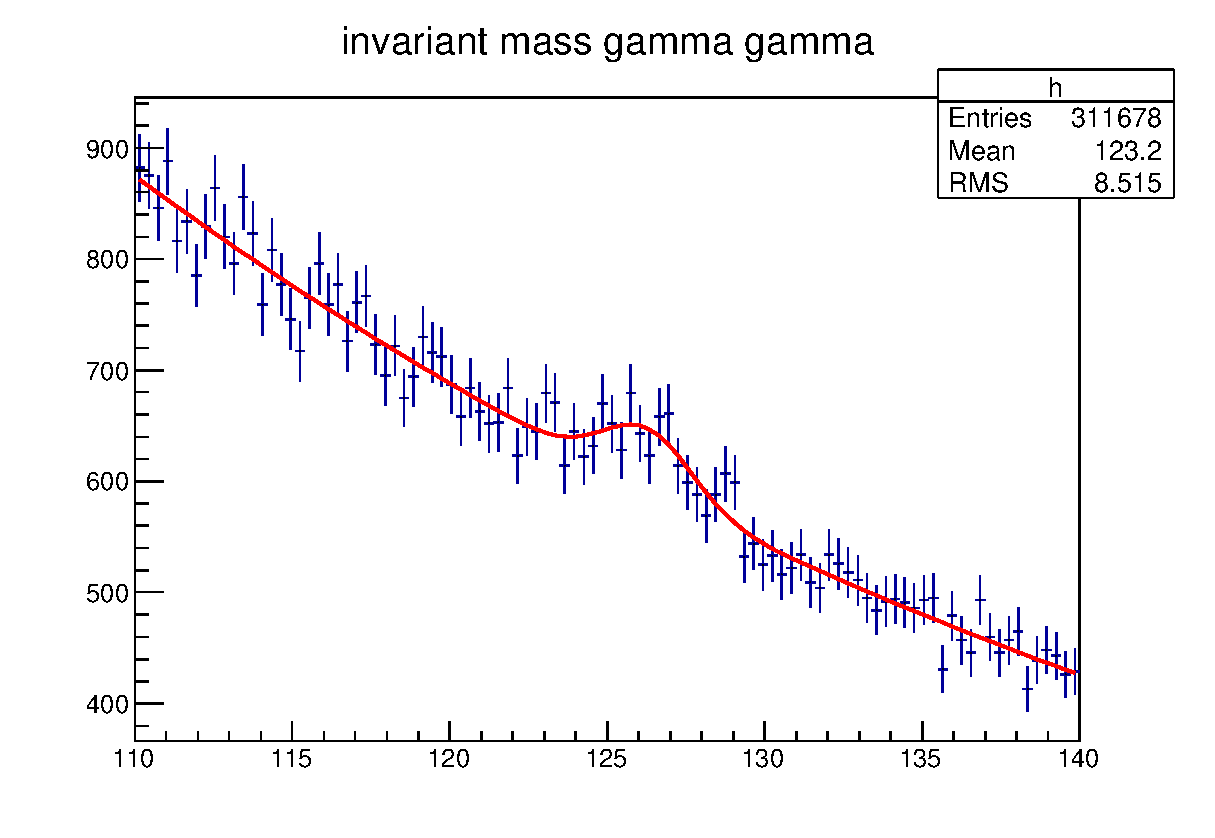
\includegraphics{../graphes/mgg_30GeV}
%\end{figure}
%
%On peut en déduire les paramètres physiquement intéressants suivants :
%
%\begin{tabular}{|l|c|r|} 
%   \hline
%   Paramètre & Valeur & Erreur \\
%    \hline
%   $E_0$ & 126,3 GeV & 0,3 GeV\\
%  \hline
%   $\sigma$ & 2,0 GeV & 0,9 GeV \\
%  \hline
%\end{tabular}
%
%La valeur $E_0$ doit correspondre à la masse du Higgs. On remarque qu'elle en est en effet bien proche (126 au lieu de 125 GeV). La valeur $\sigma$ doit correspondre à la largeur du signal, dont la valeur théorique attendue n'est pas nulle.
%
%On calcule de plus $\chi^2 = $ 68,8 pour un nombre de degrés de liberté égal à 99, ce qui correspond à une p-value de 99,0 \% (2,5$\sigma$?)
%$\Delta \chi^2 = \chi^2_{\textrm{background}} - \chi^2{\textrm{signal+background} \simeq 120-70 \simeq 50$ soit une significance à $\sqrt{\Delta \chi^2} \sigma = 7 \sigma$

Afin d'extraire le signal correspondant au Higgs, on se restreint à la plage où il est attendu (100 - 150 GeV). Le 'background' y suit une forme exponentielle. On en réalise alors un fit sur une zone ou le signal est considéré nul : ici on a choisi [100;120] $\cup$  [130;150]. On obtient une fonction de la forme $\textrm{background} = E \mapsto \exp(\xi + \epsilon E)$.

Puis, sur la plage complète ([100, 150]), on réalise un fit des données à partir d'une fonction de la forme signal+background : $E \mapsto  A \exp\left(-(E-E_0)^2/2\sigma^2\right) + \exp(\xi + \epsilon E)$

On obtient la figure suivante :

\begin{figure}[H]
\centering
  \caption{Distribution $m_{\gamma \gamma}$ et fit background+signal. }
 \resizebox{.9\linewidth}{!}{\begin{tikzpicture}
\pgfdeclareplotmark{cross} {
\pgfpathmoveto{\pgfpoint{-0.3\pgfplotmarksize}{\pgfplotmarksize}}
\pgfpathlineto{\pgfpoint{+0.3\pgfplotmarksize}{\pgfplotmarksize}}
\pgfpathlineto{\pgfpoint{+0.3\pgfplotmarksize}{0.3\pgfplotmarksize}}
\pgfpathlineto{\pgfpoint{+1\pgfplotmarksize}{0.3\pgfplotmarksize}}
\pgfpathlineto{\pgfpoint{+1\pgfplotmarksize}{-0.3\pgfplotmarksize}}
\pgfpathlineto{\pgfpoint{+0.3\pgfplotmarksize}{-0.3\pgfplotmarksize}}
\pgfpathlineto{\pgfpoint{+0.3\pgfplotmarksize}{-1.\pgfplotmarksize}}
\pgfpathlineto{\pgfpoint{-0.3\pgfplotmarksize}{-1.\pgfplotmarksize}}
\pgfpathlineto{\pgfpoint{-0.3\pgfplotmarksize}{-0.3\pgfplotmarksize}}
\pgfpathlineto{\pgfpoint{-1.\pgfplotmarksize}{-0.3\pgfplotmarksize}}
\pgfpathlineto{\pgfpoint{-1.\pgfplotmarksize}{0.3\pgfplotmarksize}}
\pgfpathlineto{\pgfpoint{-0.3\pgfplotmarksize}{0.3\pgfplotmarksize}}
\pgfpathclose
\pgfusepathqstroke
}
\pgfdeclareplotmark{cross*} {
\pgfpathmoveto{\pgfpoint{-0.3\pgfplotmarksize}{\pgfplotmarksize}}
\pgfpathlineto{\pgfpoint{+0.3\pgfplotmarksize}{\pgfplotmarksize}}
\pgfpathlineto{\pgfpoint{+0.3\pgfplotmarksize}{0.3\pgfplotmarksize}}
\pgfpathlineto{\pgfpoint{+1\pgfplotmarksize}{0.3\pgfplotmarksize}}
\pgfpathlineto{\pgfpoint{+1\pgfplotmarksize}{-0.3\pgfplotmarksize}}
\pgfpathlineto{\pgfpoint{+0.3\pgfplotmarksize}{-0.3\pgfplotmarksize}}
\pgfpathlineto{\pgfpoint{+0.3\pgfplotmarksize}{-1.\pgfplotmarksize}}
\pgfpathlineto{\pgfpoint{-0.3\pgfplotmarksize}{-1.\pgfplotmarksize}}
\pgfpathlineto{\pgfpoint{-0.3\pgfplotmarksize}{-0.3\pgfplotmarksize}}
\pgfpathlineto{\pgfpoint{-1.\pgfplotmarksize}{-0.3\pgfplotmarksize}}
\pgfpathlineto{\pgfpoint{-1.\pgfplotmarksize}{0.3\pgfplotmarksize}}
\pgfpathlineto{\pgfpoint{-0.3\pgfplotmarksize}{0.3\pgfplotmarksize}}
\pgfpathclose
\pgfusepathqfillstroke
}
\pgfdeclareplotmark{newstar} {
\pgfpathmoveto{\pgfqpoint{0pt}{\pgfplotmarksize}}
\pgfpathlineto{\pgfqpointpolar{44}{0.5\pgfplotmarksize}}
\pgfpathlineto{\pgfqpointpolar{18}{\pgfplotmarksize}}
\pgfpathlineto{\pgfqpointpolar{-20}{0.5\pgfplotmarksize}}
\pgfpathlineto{\pgfqpointpolar{-54}{\pgfplotmarksize}}
\pgfpathlineto{\pgfqpointpolar{-90}{0.5\pgfplotmarksize}}
\pgfpathlineto{\pgfqpointpolar{234}{\pgfplotmarksize}}
\pgfpathlineto{\pgfqpointpolar{198}{0.5\pgfplotmarksize}}
\pgfpathlineto{\pgfqpointpolar{162}{\pgfplotmarksize}}
\pgfpathlineto{\pgfqpointpolar{134}{0.5\pgfplotmarksize}}
\pgfpathclose
\pgfusepathqstroke
}
\pgfdeclareplotmark{newstar*} {
\pgfpathmoveto{\pgfqpoint{0pt}{\pgfplotmarksize}}
\pgfpathlineto{\pgfqpointpolar{44}{0.5\pgfplotmarksize}}
\pgfpathlineto{\pgfqpointpolar{18}{\pgfplotmarksize}}
\pgfpathlineto{\pgfqpointpolar{-20}{0.5\pgfplotmarksize}}
\pgfpathlineto{\pgfqpointpolar{-54}{\pgfplotmarksize}}
\pgfpathlineto{\pgfqpointpolar{-90}{0.5\pgfplotmarksize}}
\pgfpathlineto{\pgfqpointpolar{234}{\pgfplotmarksize}}
\pgfpathlineto{\pgfqpointpolar{198}{0.5\pgfplotmarksize}}
\pgfpathlineto{\pgfqpointpolar{162}{\pgfplotmarksize}}
\pgfpathlineto{\pgfqpointpolar{134}{0.5\pgfplotmarksize}}
\pgfpathclose
\pgfusepathqfillstroke
}
\definecolor{c}{rgb}{1,1,1};
\draw [color=c, fill=c] (0,0) rectangle (20,13.6207);
\draw [color=c, fill=c] (2,1.36207) rectangle (18,12.2586);
\definecolor{c}{rgb}{0,0,0};
\draw [c,line width=0.9] (2,1.36207) -- (2,12.2586) -- (18,12.2586) -- (18,1.36207) -- (2,1.36207);
\definecolor{c}{rgb}{1,1,1};
\draw [color=c, fill=c] (2,1.36207) rectangle (18,12.2586);
\definecolor{c}{rgb}{0,0,0};
\draw [c,line width=0.9] (2,1.36207) -- (2,12.2586) -- (18,12.2586) -- (18,1.36207) -- (2,1.36207);
\definecolor{c}{rgb}{0,0,0.6};
\draw [c,line width=0.9] (2.08,10.3742) -- (2.08,10.6675);
\draw [c,line width=0.9] (2.08,10.6675) -- (2.08,10.9608);
\draw [c,line width=0.9] (2,10.6675) -- (2.08,10.6675);
\draw [c,line width=0.9] (2.08,10.6675) -- (2.16,10.6675);
\definecolor{c}{rgb}{0,0,0};
\foreach \P in {(2.08,10.6675)}{\draw[mark options={color=c,fill=c},mark size=2.402402pt,mark=*,mark size=1pt] plot coordinates {\P};}
\definecolor{c}{rgb}{0,0,0.6};
\draw [c,line width=0.9] (2.24,11.1352) -- (2.24,11.4375);
\draw [c,line width=0.9] (2.24,11.4375) -- (2.24,11.7397);
\draw [c,line width=0.9] (2.16,11.4375) -- (2.24,11.4375);
\draw [c,line width=0.9] (2.24,11.4375) -- (2.32,11.4375);
\definecolor{c}{rgb}{0,0,0};
\foreach \P in {(2.24,11.4375)}{\draw[mark options={color=c,fill=c},mark size=2.402402pt,mark=*,mark size=1pt] plot coordinates {\P};}
\definecolor{c}{rgb}{0,0,0.6};
\draw [c,line width=0.9] (2.4,9.90813) -- (2.4,10.1958);
\draw [c,line width=0.9] (2.4,10.1958) -- (2.4,10.4835);
\draw [c,line width=0.9] (2.32,10.1958) -- (2.4,10.1958);
\draw [c,line width=0.9] (2.4,10.1958) -- (2.48,10.1958);
\definecolor{c}{rgb}{0,0,0};
\foreach \P in {(2.4,10.1958)}{\draw[mark options={color=c,fill=c},mark size=2.402402pt,mark=*,mark size=1pt] plot coordinates {\P};}
\definecolor{c}{rgb}{0,0,0.6};
\draw [c,line width=0.9] (2.56,10.1137) -- (2.56,10.4039);
\draw [c,line width=0.9] (2.56,10.4039) -- (2.56,10.6941);
\draw [c,line width=0.9] (2.48,10.4039) -- (2.56,10.4039);
\draw [c,line width=0.9] (2.56,10.4039) -- (2.64,10.4039);
\definecolor{c}{rgb}{0,0,0};
\foreach \P in {(2.56,10.4039)}{\draw[mark options={color=c,fill=c},mark size=2.402402pt,mark=*,mark size=1pt] plot coordinates {\P};}
\definecolor{c}{rgb}{0,0,0.6};
\draw [c,line width=0.9] (2.72,10.3536) -- (2.72,10.6467);
\draw [c,line width=0.9] (2.72,10.6467) -- (2.72,10.9398);
\draw [c,line width=0.9] (2.64,10.6467) -- (2.72,10.6467);
\draw [c,line width=0.9] (2.72,10.6467) -- (2.8,10.6467);
\definecolor{c}{rgb}{0,0,0};
\foreach \P in {(2.72,10.6467)}{\draw[mark options={color=c,fill=c},mark size=2.402402pt,mark=*,mark size=1pt] plot coordinates {\P};}
\definecolor{c}{rgb}{0,0,0.6};
\draw [c,line width=0.9] (2.88,10.0041) -- (2.88,10.2929);
\draw [c,line width=0.9] (2.88,10.2929) -- (2.88,10.5818);
\draw [c,line width=0.9] (2.8,10.2929) -- (2.88,10.2929);
\draw [c,line width=0.9] (2.88,10.2929) -- (2.96,10.2929);
\definecolor{c}{rgb}{0,0,0};
\foreach \P in {(2.88,10.2929)}{\draw[mark options={color=c,fill=c},mark size=2.402402pt,mark=*,mark size=1pt] plot coordinates {\P};}
\definecolor{c}{rgb}{0,0,0.6};
\draw [c,line width=0.9] (3.04,9.53811) -- (3.04,9.82124);
\draw [c,line width=0.9] (3.04,9.82124) -- (3.04,10.1044);
\draw [c,line width=0.9] (2.96,9.82124) -- (3.04,9.82124);
\draw [c,line width=0.9] (3.04,9.82124) -- (3.12,9.82124);
\definecolor{c}{rgb}{0,0,0};
\foreach \P in {(3.04,9.82124)}{\draw[mark options={color=c,fill=c},mark size=2.402402pt,mark=*,mark size=1pt] plot coordinates {\P};}
\definecolor{c}{rgb}{0,0,0.6};
\draw [c,line width=0.9] (3.2,9.5107) -- (3.2,9.79349);
\draw [c,line width=0.9] (3.2,9.79349) -- (3.2,10.0763);
\draw [c,line width=0.9] (3.12,9.79349) -- (3.2,9.79349);
\draw [c,line width=0.9] (3.2,9.79349) -- (3.28,9.79349);
\definecolor{c}{rgb}{0,0,0};
\foreach \P in {(3.2,9.79349)}{\draw[mark options={color=c,fill=c},mark size=2.402402pt,mark=*,mark size=1pt] plot coordinates {\P};}
\definecolor{c}{rgb}{0,0,0.6};
\draw [c,line width=0.9] (3.36,9.54496) -- (3.36,9.82817);
\draw [c,line width=0.9] (3.36,9.82817) -- (3.36,10.1114);
\draw [c,line width=0.9] (3.28,9.82817) -- (3.36,9.82817);
\draw [c,line width=0.9] (3.36,9.82817) -- (3.44,9.82817);
\definecolor{c}{rgb}{0,0,0};
\foreach \P in {(3.36,9.82817)}{\draw[mark options={color=c,fill=c},mark size=2.402402pt,mark=*,mark size=1pt] plot coordinates {\P};}
\definecolor{c}{rgb}{0,0,0.6};
\draw [c,line width=0.9] (3.52,9.97666) -- (3.52,10.2652);
\draw [c,line width=0.9] (3.52,10.2652) -- (3.52,10.5537);
\draw [c,line width=0.9] (3.44,10.2652) -- (3.52,10.2652);
\draw [c,line width=0.9] (3.52,10.2652) -- (3.6,10.2652);
\definecolor{c}{rgb}{0,0,0};
\foreach \P in {(3.52,10.2652)}{\draw[mark options={color=c,fill=c},mark size=2.402402pt,mark=*,mark size=1pt] plot coordinates {\P};}
\definecolor{c}{rgb}{0,0,0.6};
\draw [c,line width=0.9] (3.68,9.44219) -- (3.68,9.72412);
\draw [c,line width=0.9] (3.68,9.72412) -- (3.68,10.0061);
\draw [c,line width=0.9] (3.6,9.72412) -- (3.68,9.72412);
\draw [c,line width=0.9] (3.68,9.72412) -- (3.76,9.72412);
\definecolor{c}{rgb}{0,0,0};
\foreach \P in {(3.68,9.72412)}{\draw[mark options={color=c,fill=c},mark size=2.402402pt,mark=*,mark size=1pt] plot coordinates {\P};}
\definecolor{c}{rgb}{0,0,0.6};
\draw [c,line width=0.9] (3.84,9.33257) -- (3.84,9.61314);
\draw [c,line width=0.9] (3.84,9.61314) -- (3.84,9.89371);
\draw [c,line width=0.9] (3.76,9.61314) -- (3.84,9.61314);
\draw [c,line width=0.9] (3.84,9.61314) -- (3.92,9.61314);
\definecolor{c}{rgb}{0,0,0};
\foreach \P in {(3.84,9.61314)}{\draw[mark options={color=c,fill=c},mark size=2.402402pt,mark=*,mark size=1pt] plot coordinates {\P};}
\definecolor{c}{rgb}{0,0,0.6};
\draw [c,line width=0.9] (4,9.18186) -- (4,9.46053);
\draw [c,line width=0.9] (4,9.46053) -- (4,9.73921);
\draw [c,line width=0.9] (3.92,9.46053) -- (4,9.46053);
\draw [c,line width=0.9] (4,9.46053) -- (4.08,9.46053);
\definecolor{c}{rgb}{0,0,0};
\foreach \P in {(4,9.46053)}{\draw[mark options={color=c,fill=c},mark size=2.402402pt,mark=*,mark size=1pt] plot coordinates {\P};}
\definecolor{c}{rgb}{0,0,0.6};
\draw [c,line width=0.9] (4.16,8.4285) -- (4.16,8.69751);
\draw [c,line width=0.9] (4.16,8.69751) -- (4.16,8.96652);
\draw [c,line width=0.9] (4.08,8.69751) -- (4.16,8.69751);
\draw [c,line width=0.9] (4.16,8.69751) -- (4.24,8.69751);
\definecolor{c}{rgb}{0,0,0};
\foreach \P in {(4.16,8.69751)}{\draw[mark options={color=c,fill=c},mark size=2.402402pt,mark=*,mark size=1pt] plot coordinates {\P};}
\definecolor{c}{rgb}{0,0,0.6};
\draw [c,line width=0.9] (4.32,8.61338) -- (4.32,8.8848);
\draw [c,line width=0.9] (4.32,8.8848) -- (4.32,9.15621);
\draw [c,line width=0.9] (4.24,8.8848) -- (4.32,8.8848);
\draw [c,line width=0.9] (4.32,8.8848) -- (4.4,8.8848);
\definecolor{c}{rgb}{0,0,0};
\foreach \P in {(4.32,8.8848)}{\draw[mark options={color=c,fill=c},mark size=2.402402pt,mark=*,mark size=1pt] plot coordinates {\P};}
\definecolor{c}{rgb}{0,0,0.6};
\draw [c,line width=0.9] (4.48,8.5449) -- (4.48,8.81543);
\draw [c,line width=0.9] (4.48,8.81543) -- (4.48,9.08596);
\draw [c,line width=0.9] (4.4,8.81543) -- (4.48,8.81543);
\draw [c,line width=0.9] (4.48,8.81543) -- (4.56,8.81543);
\definecolor{c}{rgb}{0,0,0};
\foreach \P in {(4.48,8.81543)}{\draw[mark options={color=c,fill=c},mark size=2.402402pt,mark=*,mark size=1pt] plot coordinates {\P};}
\definecolor{c}{rgb}{0,0,0.6};
\draw [c,line width=0.9] (4.64,8.68871) -- (4.64,8.9611);
\draw [c,line width=0.9] (4.64,8.9611) -- (4.64,9.23349);
\draw [c,line width=0.9] (4.56,8.9611) -- (4.64,8.9611);
\draw [c,line width=0.9] (4.64,8.9611) -- (4.72,8.9611);
\definecolor{c}{rgb}{0,0,0};
\foreach \P in {(4.64,8.9611)}{\draw[mark options={color=c,fill=c},mark size=2.402402pt,mark=*,mark size=1pt] plot coordinates {\P};}
\definecolor{c}{rgb}{0,0,0.6};
\draw [c,line width=0.9] (4.8,8.33949) -- (4.8,8.60733);
\draw [c,line width=0.9] (4.8,8.60733) -- (4.8,8.87518);
\draw [c,line width=0.9] (4.72,8.60733) -- (4.8,8.60733);
\draw [c,line width=0.9] (4.8,8.60733) -- (4.88,8.60733);
\definecolor{c}{rgb}{0,0,0};
\foreach \P in {(4.8,8.60733)}{\draw[mark options={color=c,fill=c},mark size=2.402402pt,mark=*,mark size=1pt] plot coordinates {\P};}
\definecolor{c}{rgb}{0,0,0.6};
\draw [c,line width=0.9] (4.96,8.09303) -- (4.96,8.35762);
\draw [c,line width=0.9] (4.96,8.35762) -- (4.96,8.62221);
\draw [c,line width=0.9] (4.88,8.35762) -- (4.96,8.35762);
\draw [c,line width=0.9] (4.96,8.35762) -- (5.04,8.35762);
\definecolor{c}{rgb}{0,0,0};
\foreach \P in {(4.96,8.35762)}{\draw[mark options={color=c,fill=c},mark size=2.402402pt,mark=*,mark size=1pt] plot coordinates {\P};}
\definecolor{c}{rgb}{0,0,0.6};
\draw [c,line width=0.9] (5.12,8.63393) -- (5.12,8.90561);
\draw [c,line width=0.9] (5.12,8.90561) -- (5.12,9.17729);
\draw [c,line width=0.9] (5.04,8.90561) -- (5.12,8.90561);
\draw [c,line width=0.9] (5.12,8.90561) -- (5.2,8.90561);
\definecolor{c}{rgb}{0,0,0};
\foreach \P in {(5.12,8.90561)}{\draw[mark options={color=c,fill=c},mark size=2.402402pt,mark=*,mark size=1pt] plot coordinates {\P};}
\definecolor{c}{rgb}{0,0,0.6};
\draw [c,line width=0.9] (5.28,8.09987) -- (5.28,8.36455);
\draw [c,line width=0.9] (5.28,8.36455) -- (5.28,8.62924);
\draw [c,line width=0.9] (5.2,8.36455) -- (5.28,8.36455);
\draw [c,line width=0.9] (5.28,8.36455) -- (5.36,8.36455);
\definecolor{c}{rgb}{0,0,0};
\foreach \P in {(5.28,8.36455)}{\draw[mark options={color=c,fill=c},mark size=2.402402pt,mark=*,mark size=1pt] plot coordinates {\P};}
\definecolor{c}{rgb}{0,0,0.6};
\draw [c,line width=0.9] (5.44,8.20256) -- (5.44,8.4686);
\draw [c,line width=0.9] (5.44,8.4686) -- (5.44,8.73464);
\draw [c,line width=0.9] (5.36,8.4686) -- (5.44,8.4686);
\draw [c,line width=0.9] (5.44,8.4686) -- (5.52,8.4686);
\definecolor{c}{rgb}{0,0,0};
\foreach \P in {(5.44,8.4686)}{\draw[mark options={color=c,fill=c},mark size=2.402402pt,mark=*,mark size=1pt] plot coordinates {\P};}
\definecolor{c}{rgb}{0,0,0.6};
\draw [c,line width=0.9] (5.6,7.57969) -- (5.6,7.83737);
\draw [c,line width=0.9] (5.6,7.83737) -- (5.6,8.09506);
\draw [c,line width=0.9] (5.52,7.83737) -- (5.6,7.83737);
\draw [c,line width=0.9] (5.6,7.83737) -- (5.68,7.83737);
\definecolor{c}{rgb}{0,0,0};
\foreach \P in {(5.6,7.83737)}{\draw[mark options={color=c,fill=c},mark size=2.402402pt,mark=*,mark size=1pt] plot coordinates {\P};}
\definecolor{c}{rgb}{0,0,0.6};
\draw [c,line width=0.9] (5.76,7.49758) -- (5.76,7.75413);
\draw [c,line width=0.9] (5.76,7.75413) -- (5.76,8.01069);
\draw [c,line width=0.9] (5.68,7.75413) -- (5.76,7.75413);
\draw [c,line width=0.9] (5.76,7.75413) -- (5.84,7.75413);
\definecolor{c}{rgb}{0,0,0};
\foreach \P in {(5.76,7.75413)}{\draw[mark options={color=c,fill=c},mark size=2.402402pt,mark=*,mark size=1pt] plot coordinates {\P};}
\definecolor{c}{rgb}{0,0,0.6};
\draw [c,line width=0.9] (5.92,7.4702) -- (5.92,7.72639);
\draw [c,line width=0.9] (5.92,7.72639) -- (5.92,7.98257);
\draw [c,line width=0.9] (5.84,7.72639) -- (5.92,7.72639);
\draw [c,line width=0.9] (5.92,7.72639) -- (6,7.72639);
\definecolor{c}{rgb}{0,0,0};
\foreach \P in {(5.92,7.72639)}{\draw[mark options={color=c,fill=c},mark size=2.402402pt,mark=*,mark size=1pt] plot coordinates {\P};}
\definecolor{c}{rgb}{0,0,0.6};
\draw [c,line width=0.9] (6.08,7.71656) -- (6.08,7.97611);
\draw [c,line width=0.9] (6.08,7.97611) -- (6.08,8.23565);
\draw [c,line width=0.9] (6,7.97611) -- (6.08,7.97611);
\draw [c,line width=0.9] (6.08,7.97611) -- (6.16,7.97611);
\definecolor{c}{rgb}{0,0,0};
\foreach \P in {(6.08,7.97611)}{\draw[mark options={color=c,fill=c},mark size=2.402402pt,mark=*,mark size=1pt] plot coordinates {\P};}
\definecolor{c}{rgb}{0,0,0.6};
\draw [c,line width=0.9] (6.24,7.57969) -- (6.24,7.83737);
\draw [c,line width=0.9] (6.24,7.83737) -- (6.24,8.09506);
\draw [c,line width=0.9] (6.16,7.83737) -- (6.24,7.83737);
\draw [c,line width=0.9] (6.24,7.83737) -- (6.32,7.83737);
\definecolor{c}{rgb}{0,0,0};
\foreach \P in {(6.24,7.83737)}{\draw[mark options={color=c,fill=c},mark size=2.402402pt,mark=*,mark size=1pt] plot coordinates {\P};}
\definecolor{c}{rgb}{0,0,0.6};
\draw [c,line width=0.9] (6.4,7.53179) -- (6.4,7.78882);
\draw [c,line width=0.9] (6.4,7.78882) -- (6.4,8.04585);
\draw [c,line width=0.9] (6.32,7.78882) -- (6.4,7.78882);
\draw [c,line width=0.9] (6.4,7.78882) -- (6.48,7.78882);
\definecolor{c}{rgb}{0,0,0};
\foreach \P in {(6.4,7.78882)}{\draw[mark options={color=c,fill=c},mark size=2.402402pt,mark=*,mark size=1pt] plot coordinates {\P};}
\definecolor{c}{rgb}{0,0,0.6};
\draw [c,line width=0.9] (6.56,6.9571) -- (6.56,7.20615);
\draw [c,line width=0.9] (6.56,7.20615) -- (6.56,7.45519);
\draw [c,line width=0.9] (6.48,7.20615) -- (6.56,7.20615);
\draw [c,line width=0.9] (6.56,7.20615) -- (6.64,7.20615);
\definecolor{c}{rgb}{0,0,0};
\foreach \P in {(6.56,7.20615)}{\draw[mark options={color=c,fill=c},mark size=2.402402pt,mark=*,mark size=1pt] plot coordinates {\P};}
\definecolor{c}{rgb}{0,0,0.6};
\draw [c,line width=0.9] (6.72,6.7656) -- (6.72,7.01192);
\draw [c,line width=0.9] (6.72,7.01192) -- (6.72,7.25824);
\draw [c,line width=0.9] (6.64,7.01192) -- (6.72,7.01192);
\draw [c,line width=0.9] (6.72,7.01192) -- (6.8,7.01192);
\definecolor{c}{rgb}{0,0,0};
\foreach \P in {(6.72,7.01192)}{\draw[mark options={color=c,fill=c},mark size=2.402402pt,mark=*,mark size=1pt] plot coordinates {\P};}
\definecolor{c}{rgb}{0,0,0.6};
\draw [c,line width=0.9] (6.88,6.44421) -- (6.88,6.6859);
\draw [c,line width=0.9] (6.88,6.6859) -- (6.88,6.92759);
\draw [c,line width=0.9] (6.8,6.6859) -- (6.88,6.6859);
\draw [c,line width=0.9] (6.88,6.6859) -- (6.96,6.6859);
\definecolor{c}{rgb}{0,0,0};
\foreach \P in {(6.88,6.6859)}{\draw[mark options={color=c,fill=c},mark size=2.402402pt,mark=*,mark size=1pt] plot coordinates {\P};}
\definecolor{c}{rgb}{0,0,0.6};
\draw [c,line width=0.9] (7.04,7.21021) -- (7.04,7.4628);
\draw [c,line width=0.9] (7.04,7.4628) -- (7.04,7.71539);
\draw [c,line width=0.9] (6.96,7.4628) -- (7.04,7.4628);
\draw [c,line width=0.9] (7.04,7.4628) -- (7.12,7.4628);
\definecolor{c}{rgb}{0,0,0};
\foreach \P in {(7.04,7.4628)}{\draw[mark options={color=c,fill=c},mark size=2.402402pt,mark=*,mark size=1pt] plot coordinates {\P};}
\definecolor{c}{rgb}{0,0,0.6};
\draw [c,line width=0.9] (7.2,6.92974) -- (7.2,7.1784);
\draw [c,line width=0.9] (7.2,7.1784) -- (7.2,7.42705);
\draw [c,line width=0.9] (7.12,7.1784) -- (7.2,7.1784);
\draw [c,line width=0.9] (7.2,7.1784) -- (7.28,7.1784);
\definecolor{c}{rgb}{0,0,0};
\foreach \P in {(7.2,7.1784)}{\draw[mark options={color=c,fill=c},mark size=2.402402pt,mark=*,mark size=1pt] plot coordinates {\P};}
\definecolor{c}{rgb}{0,0,0.6};
\draw [c,line width=0.9] (7.36,6.60148) -- (7.36,6.84544);
\draw [c,line width=0.9] (7.36,6.84544) -- (7.36,7.08941);
\draw [c,line width=0.9] (7.28,6.84544) -- (7.36,6.84544);
\draw [c,line width=0.9] (7.36,6.84544) -- (7.44,6.84544);
\definecolor{c}{rgb}{0,0,0};
\foreach \P in {(7.36,6.84544)}{\draw[mark options={color=c,fill=c},mark size=2.402402pt,mark=*,mark size=1pt] plot coordinates {\P};}
\definecolor{c}{rgb}{0,0,0.6};
\draw [c,line width=0.9] (7.52,6.81347) -- (7.52,7.06048);
\draw [c,line width=0.9] (7.52,7.06048) -- (7.52,7.30748);
\draw [c,line width=0.9] (7.44,7.06048) -- (7.52,7.06048);
\draw [c,line width=0.9] (7.52,7.06048) -- (7.6,7.06048);
\definecolor{c}{rgb}{0,0,0};
\foreach \P in {(7.52,7.06048)}{\draw[mark options={color=c,fill=c},mark size=2.402402pt,mark=*,mark size=1pt] plot coordinates {\P};}
\definecolor{c}{rgb}{0,0,0.6};
\draw [c,line width=0.9] (7.68,6.21178) -- (7.68,6.45006);
\draw [c,line width=0.9] (7.68,6.45006) -- (7.68,6.68834);
\draw [c,line width=0.9] (7.6,6.45006) -- (7.68,6.45006);
\draw [c,line width=0.9] (7.68,6.45006) -- (7.76,6.45006);
\definecolor{c}{rgb}{0,0,0};
\foreach \P in {(7.68,6.45006)}{\draw[mark options={color=c,fill=c},mark size=2.402402pt,mark=*,mark size=1pt] plot coordinates {\P};}
\definecolor{c}{rgb}{0,0,0.6};
\draw [c,line width=0.9] (7.84,6.25279) -- (7.84,6.49168);
\draw [c,line width=0.9] (7.84,6.49168) -- (7.84,6.73056);
\draw [c,line width=0.9] (7.76,6.49168) -- (7.84,6.49168);
\draw [c,line width=0.9] (7.84,6.49168) -- (7.92,6.49168);
\definecolor{c}{rgb}{0,0,0};
\foreach \P in {(7.84,6.49168)}{\draw[mark options={color=c,fill=c},mark size=2.402402pt,mark=*,mark size=1pt] plot coordinates {\P};}
\definecolor{c}{rgb}{0,0,0.6};
\draw [c,line width=0.9] (8,5.95889) -- (8,6.1934);
\draw [c,line width=0.9] (8,6.1934) -- (8,6.42792);
\draw [c,line width=0.9] (7.92,6.1934) -- (8,6.1934);
\draw [c,line width=0.9] (8,6.1934) -- (8.08,6.1934);
\definecolor{c}{rgb}{0,0,0};
\foreach \P in {(8,6.1934)}{\draw[mark options={color=c,fill=c},mark size=2.402402pt,mark=*,mark size=1pt] plot coordinates {\P};}
\definecolor{c}{rgb}{0,0,0.6};
\draw [c,line width=0.9] (8.16,6.5878) -- (8.16,6.83157);
\draw [c,line width=0.9] (8.16,6.83157) -- (8.16,7.07534);
\draw [c,line width=0.9] (8.08,6.83157) -- (8.16,6.83157);
\draw [c,line width=0.9] (8.16,6.83157) -- (8.24,6.83157);
\definecolor{c}{rgb}{0,0,0};
\foreach \P in {(8.16,6.83157)}{\draw[mark options={color=c,fill=c},mark size=2.402402pt,mark=*,mark size=1pt] plot coordinates {\P};}
\definecolor{c}{rgb}{0,0,0.6};
\draw [c,line width=0.9] (8.32,6.10241) -- (8.32,6.33907);
\draw [c,line width=0.9] (8.32,6.33907) -- (8.32,6.57573);
\draw [c,line width=0.9] (8.24,6.33907) -- (8.32,6.33907);
\draw [c,line width=0.9] (8.32,6.33907) -- (8.4,6.33907);
\definecolor{c}{rgb}{0,0,0};
\foreach \P in {(8.32,6.33907)}{\draw[mark options={color=c,fill=c},mark size=2.402402pt,mark=*,mark size=1pt] plot coordinates {\P};}
\definecolor{c}{rgb}{0,0,0.6};
\draw [c,line width=0.9] (8.48,5.6924) -- (8.48,5.92288);
\draw [c,line width=0.9] (8.48,5.92288) -- (8.48,6.15336);
\draw [c,line width=0.9] (8.4,5.92288) -- (8.48,5.92288);
\draw [c,line width=0.9] (8.48,5.92288) -- (8.56,5.92288);
\definecolor{c}{rgb}{0,0,0};
\foreach \P in {(8.48,5.92288)}{\draw[mark options={color=c,fill=c},mark size=2.402402pt,mark=*,mark size=1pt] plot coordinates {\P};}
\definecolor{c}{rgb}{0,0,0.6};
\draw [c,line width=0.9] (8.64,5.80172) -- (8.64,6.03386);
\draw [c,line width=0.9] (8.64,6.03386) -- (8.64,6.26601);
\draw [c,line width=0.9] (8.56,6.03386) -- (8.64,6.03386);
\draw [c,line width=0.9] (8.64,6.03386) -- (8.72,6.03386);
\definecolor{c}{rgb}{0,0,0};
\foreach \P in {(8.64,6.03386)}{\draw[mark options={color=c,fill=c},mark size=2.402402pt,mark=*,mark size=1pt] plot coordinates {\P};}
\definecolor{c}{rgb}{0,0,0.6};
\draw [c,line width=0.9] (8.8,5.55577) -- (8.8,5.78415);
\draw [c,line width=0.9] (8.8,5.78415) -- (8.8,6.01253);
\draw [c,line width=0.9] (8.72,5.78415) -- (8.8,5.78415);
\draw [c,line width=0.9] (8.8,5.78415) -- (8.88,5.78415);
\definecolor{c}{rgb}{0,0,0};
\foreach \P in {(8.8,5.78415)}{\draw[mark options={color=c,fill=c},mark size=2.402402pt,mark=*,mark size=1pt] plot coordinates {\P};}
\definecolor{c}{rgb}{0,0,0.6};
\draw [c,line width=0.9] (8.96,5.88372) -- (8.96,6.1171);
\draw [c,line width=0.9] (8.96,6.1171) -- (8.96,6.35048);
\draw [c,line width=0.9] (8.88,6.1171) -- (8.96,6.1171);
\draw [c,line width=0.9] (8.96,6.1171) -- (9.04,6.1171);
\definecolor{c}{rgb}{0,0,0};
\foreach \P in {(8.96,6.1171)}{\draw[mark options={color=c,fill=c},mark size=2.402402pt,mark=*,mark size=1pt] plot coordinates {\P};}
\definecolor{c}{rgb}{0,0,0.6};
\draw [c,line width=0.9] (9.12,5.385) -- (9.12,5.61073);
\draw [c,line width=0.9] (9.12,5.61073) -- (9.12,5.83646);
\draw [c,line width=0.9] (9.04,5.61073) -- (9.12,5.61073);
\draw [c,line width=0.9] (9.12,5.61073) -- (9.2,5.61073);
\definecolor{c}{rgb}{0,0,0};
\foreach \P in {(9.12,5.61073)}{\draw[mark options={color=c,fill=c},mark size=2.402402pt,mark=*,mark size=1pt] plot coordinates {\P};}
\definecolor{c}{rgb}{0,0,0.6};
\draw [c,line width=0.9] (9.28,5.6719) -- (9.28,5.90207);
\draw [c,line width=0.9] (9.28,5.90207) -- (9.28,6.13223);
\draw [c,line width=0.9] (9.2,5.90207) -- (9.28,5.90207);
\draw [c,line width=0.9] (9.28,5.90207) -- (9.36,5.90207);
\definecolor{c}{rgb}{0,0,0};
\foreach \P in {(9.28,5.90207)}{\draw[mark options={color=c,fill=c},mark size=2.402402pt,mark=*,mark size=1pt] plot coordinates {\P};}
\definecolor{c}{rgb}{0,0,0.6};
\draw [c,line width=0.9] (9.44,5.7129) -- (9.44,5.94369);
\draw [c,line width=0.9] (9.44,5.94369) -- (9.44,6.17448);
\draw [c,line width=0.9] (9.36,5.94369) -- (9.44,5.94369);
\draw [c,line width=0.9] (9.44,5.94369) -- (9.52,5.94369);
\definecolor{c}{rgb}{0,0,0};
\foreach \P in {(9.44,5.94369)}{\draw[mark options={color=c,fill=c},mark size=2.402402pt,mark=*,mark size=1pt] plot coordinates {\P};}
\definecolor{c}{rgb}{0,0,0.6};
\draw [c,line width=0.9] (9.6,5.16647) -- (9.6,5.38876);
\draw [c,line width=0.9] (9.6,5.38876) -- (9.6,5.61106);
\draw [c,line width=0.9] (9.52,5.38876) -- (9.6,5.38876);
\draw [c,line width=0.9] (9.6,5.38876) -- (9.68,5.38876);
\definecolor{c}{rgb}{0,0,0};
\foreach \P in {(9.6,5.38876)}{\draw[mark options={color=c,fill=c},mark size=2.402402pt,mark=*,mark size=1pt] plot coordinates {\P};}
\definecolor{c}{rgb}{0,0,0.6};
\draw [c,line width=0.9] (9.76,5.46696) -- (9.76,5.69397);
\draw [c,line width=0.9] (9.76,5.69397) -- (9.76,5.92098);
\draw [c,line width=0.9] (9.68,5.69397) -- (9.76,5.69397);
\draw [c,line width=0.9] (9.76,5.69397) -- (9.84,5.69397);
\definecolor{c}{rgb}{0,0,0};
\foreach \P in {(9.76,5.69397)}{\draw[mark options={color=c,fill=c},mark size=2.402402pt,mark=*,mark size=1pt] plot coordinates {\P};}
\definecolor{c}{rgb}{0,0,0.6};
\draw [c,line width=0.9] (9.92,5.5626) -- (9.92,5.79108);
\draw [c,line width=0.9] (9.92,5.79108) -- (9.92,6.01957);
\draw [c,line width=0.9] (9.84,5.79108) -- (9.92,5.79108);
\draw [c,line width=0.9] (9.92,5.79108) -- (10,5.79108);
\definecolor{c}{rgb}{0,0,0};
\foreach \P in {(9.92,5.79108)}{\draw[mark options={color=c,fill=c},mark size=2.402402pt,mark=*,mark size=1pt] plot coordinates {\P};}
\definecolor{c}{rgb}{0,0,0.6};
\draw [c,line width=0.9] (10.08,5.48063) -- (10.08,5.70784);
\draw [c,line width=0.9] (10.08,5.70784) -- (10.08,5.93506);
\draw [c,line width=0.9] (10,5.70784) -- (10.08,5.70784);
\draw [c,line width=0.9] (10.08,5.70784) -- (10.16,5.70784);
\definecolor{c}{rgb}{0,0,0};
\foreach \P in {(10.08,5.70784)}{\draw[mark options={color=c,fill=c},mark size=2.402402pt,mark=*,mark size=1pt] plot coordinates {\P};}
\definecolor{c}{rgb}{0,0,0.6};
\draw [c,line width=0.9] (10.24,5.78806) -- (10.24,6.01999);
\draw [c,line width=0.9] (10.24,6.01999) -- (10.24,6.25192);
\draw [c,line width=0.9] (10.16,6.01999) -- (10.24,6.01999);
\draw [c,line width=0.9] (10.24,6.01999) -- (10.32,6.01999);
\definecolor{c}{rgb}{0,0,0};
\foreach \P in {(10.24,6.01999)}{\draw[mark options={color=c,fill=c},mark size=2.402402pt,mark=*,mark size=1pt] plot coordinates {\P};}
\definecolor{c}{rgb}{0,0,0.6};
\draw [c,line width=0.9] (10.4,5.21427) -- (10.4,5.43732);
\draw [c,line width=0.9] (10.4,5.43732) -- (10.4,5.66037);
\draw [c,line width=0.9] (10.32,5.43732) -- (10.4,5.43732);
\draw [c,line width=0.9] (10.4,5.43732) -- (10.48,5.43732);
\definecolor{c}{rgb}{0,0,0};
\foreach \P in {(10.4,5.43732)}{\draw[mark options={color=c,fill=c},mark size=2.402402pt,mark=*,mark size=1pt] plot coordinates {\P};}
\definecolor{c}{rgb}{0,0,0.6};
\draw [c,line width=0.9] (10.56,5.51478) -- (10.56,5.74253);
\draw [c,line width=0.9] (10.56,5.74253) -- (10.56,5.97027);
\draw [c,line width=0.9] (10.48,5.74253) -- (10.56,5.74253);
\draw [c,line width=0.9] (10.56,5.74253) -- (10.64,5.74253);
\definecolor{c}{rgb}{0,0,0};
\foreach \P in {(10.56,5.74253)}{\draw[mark options={color=c,fill=c},mark size=2.402402pt,mark=*,mark size=1pt] plot coordinates {\P};}
\definecolor{c}{rgb}{0,0,0.6};
\draw [c,line width=0.9] (10.72,5.36451) -- (10.72,5.58992);
\draw [c,line width=0.9] (10.72,5.58992) -- (10.72,5.81533);
\draw [c,line width=0.9] (10.64,5.58992) -- (10.72,5.58992);
\draw [c,line width=0.9] (10.72,5.58992) -- (10.8,5.58992);
\definecolor{c}{rgb}{0,0,0};
\foreach \P in {(10.72,5.58992)}{\draw[mark options={color=c,fill=c},mark size=2.402402pt,mark=*,mark size=1pt] plot coordinates {\P};}
\definecolor{c}{rgb}{0,0,0.6};
\draw [c,line width=0.9] (10.88,4.88655) -- (10.88,5.10436);
\draw [c,line width=0.9] (10.88,5.10436) -- (10.88,5.32218);
\draw [c,line width=0.9] (10.8,5.10436) -- (10.88,5.10436);
\draw [c,line width=0.9] (10.88,5.10436) -- (10.96,5.10436);
\definecolor{c}{rgb}{0,0,0};
\foreach \P in {(10.88,5.10436)}{\draw[mark options={color=c,fill=c},mark size=2.402402pt,mark=*,mark size=1pt] plot coordinates {\P};}
\definecolor{c}{rgb}{0,0,0.6};
\draw [c,line width=0.9] (11.04,4.75004) -- (11.04,4.96563);
\draw [c,line width=0.9] (11.04,4.96563) -- (11.04,5.18122);
\draw [c,line width=0.9] (10.96,4.96563) -- (11.04,4.96563);
\draw [c,line width=0.9] (11.04,4.96563) -- (11.12,4.96563);
\definecolor{c}{rgb}{0,0,0};
\foreach \P in {(11.04,4.96563)}{\draw[mark options={color=c,fill=c},mark size=2.402402pt,mark=*,mark size=1pt] plot coordinates {\P};}
\definecolor{c}{rgb}{0,0,0.6};
\draw [c,line width=0.9] (11.2,5.07087) -- (11.2,5.29165);
\draw [c,line width=0.9] (11.2,5.29165) -- (11.2,5.51242);
\draw [c,line width=0.9] (11.12,5.29165) -- (11.2,5.29165);
\draw [c,line width=0.9] (11.2,5.29165) -- (11.28,5.29165);
\definecolor{c}{rgb}{0,0,0};
\foreach \P in {(11.2,5.29165)}{\draw[mark options={color=c,fill=c},mark size=2.402402pt,mark=*,mark size=1pt] plot coordinates {\P};}
\definecolor{c}{rgb}{0,0,0.6};
\draw [c,line width=0.9] (11.36,4.40886) -- (11.36,4.6188);
\draw [c,line width=0.9] (11.36,4.6188) -- (11.36,4.82874);
\draw [c,line width=0.9] (11.28,4.6188) -- (11.36,4.6188);
\draw [c,line width=0.9] (11.36,4.6188) -- (11.44,4.6188);
\definecolor{c}{rgb}{0,0,0};
\foreach \P in {(11.36,4.6188)}{\draw[mark options={color=c,fill=c},mark size=2.402402pt,mark=*,mark size=1pt] plot coordinates {\P};}
\definecolor{c}{rgb}{0,0,0.6};
\draw [c,line width=0.9] (11.52,4.22469) -- (11.52,4.43151);
\draw [c,line width=0.9] (11.52,4.43151) -- (11.52,4.63834);
\draw [c,line width=0.9] (11.44,4.43151) -- (11.52,4.43151);
\draw [c,line width=0.9] (11.52,4.43151) -- (11.6,4.43151);
\definecolor{c}{rgb}{0,0,0};
\foreach \P in {(11.52,4.43151)}{\draw[mark options={color=c,fill=c},mark size=2.402402pt,mark=*,mark size=1pt] plot coordinates {\P};}
\definecolor{c}{rgb}{0,0,0.6};
\draw [c,line width=0.9] (11.68,4.29972) -- (11.68,4.50782);
\draw [c,line width=0.9] (11.68,4.50782) -- (11.68,4.71591);
\draw [c,line width=0.9] (11.6,4.50782) -- (11.68,4.50782);
\draw [c,line width=0.9] (11.68,4.50782) -- (11.76,4.50782);
\definecolor{c}{rgb}{0,0,0};
\foreach \P in {(11.68,4.50782)}{\draw[mark options={color=c,fill=c},mark size=2.402402pt,mark=*,mark size=1pt] plot coordinates {\P};}
\definecolor{c}{rgb}{0,0,0.6};
\draw [c,line width=0.9] (11.84,3.96557) -- (11.84,4.16792);
\draw [c,line width=0.9] (11.84,4.16792) -- (11.84,4.37028);
\draw [c,line width=0.9] (11.76,4.16792) -- (11.84,4.16792);
\draw [c,line width=0.9] (11.84,4.16792) -- (11.92,4.16792);
\definecolor{c}{rgb}{0,0,0};
\foreach \P in {(11.84,4.16792)}{\draw[mark options={color=c,fill=c},mark size=2.402402pt,mark=*,mark size=1pt] plot coordinates {\P};}
\definecolor{c}{rgb}{0,0,0.6};
\draw [c,line width=0.9] (12,4.19059) -- (12,4.39683);
\draw [c,line width=0.9] (12,4.39683) -- (12,4.60307);
\draw [c,line width=0.9] (11.92,4.39683) -- (12,4.39683);
\draw [c,line width=0.9] (12,4.39683) -- (12.08,4.39683);
\definecolor{c}{rgb}{0,0,0};
\foreach \P in {(12,4.39683)}{\draw[mark options={color=c,fill=c},mark size=2.402402pt,mark=*,mark size=1pt] plot coordinates {\P};}
\definecolor{c}{rgb}{0,0,0.6};
\draw [c,line width=0.9] (12.16,3.82923) -- (12.16,4.02919);
\draw [c,line width=0.9] (12.16,4.02919) -- (12.16,4.22915);
\draw [c,line width=0.9] (12.08,4.02919) -- (12.16,4.02919);
\draw [c,line width=0.9] (12.16,4.02919) -- (12.24,4.02919);
\definecolor{c}{rgb}{0,0,0};
\foreach \P in {(12.16,4.02919)}{\draw[mark options={color=c,fill=c},mark size=2.402402pt,mark=*,mark size=1pt] plot coordinates {\P};}
\definecolor{c}{rgb}{0,0,0.6};
\draw [c,line width=0.9] (12.32,4.24515) -- (12.32,4.45232);
\draw [c,line width=0.9] (12.32,4.45232) -- (12.32,4.65949);
\draw [c,line width=0.9] (12.24,4.45232) -- (12.32,4.45232);
\draw [c,line width=0.9] (12.32,4.45232) -- (12.4,4.45232);
\definecolor{c}{rgb}{0,0,0};
\foreach \P in {(12.32,4.45232)}{\draw[mark options={color=c,fill=c},mark size=2.402402pt,mark=*,mark size=1pt] plot coordinates {\P};}
\definecolor{c}{rgb}{0,0,0.6};
\draw [c,line width=0.9] (12.48,4.11558) -- (12.48,4.32053);
\draw [c,line width=0.9] (12.48,4.32053) -- (12.48,4.52548);
\draw [c,line width=0.9] (12.4,4.32053) -- (12.48,4.32053);
\draw [c,line width=0.9] (12.48,4.32053) -- (12.56,4.32053);
\definecolor{c}{rgb}{0,0,0};
\foreach \P in {(12.48,4.32053)}{\draw[mark options={color=c,fill=c},mark size=2.402402pt,mark=*,mark size=1pt] plot coordinates {\P};}
\definecolor{c}{rgb}{0,0,0.6};
\draw [c,line width=0.9] (12.64,3.67929) -- (12.64,3.87659);
\draw [c,line width=0.9] (12.64,3.87659) -- (12.64,4.07388);
\draw [c,line width=0.9] (12.56,3.87659) -- (12.64,3.87659);
\draw [c,line width=0.9] (12.64,3.87659) -- (12.72,3.87659);
\definecolor{c}{rgb}{0,0,0};
\foreach \P in {(12.64,3.87659)}{\draw[mark options={color=c,fill=c},mark size=2.402402pt,mark=*,mark size=1pt] plot coordinates {\P};}
\definecolor{c}{rgb}{0,0,0.6};
\draw [c,line width=0.9] (12.8,3.74063) -- (12.8,3.93902);
\draw [c,line width=0.9] (12.8,3.93902) -- (12.8,4.13741);
\draw [c,line width=0.9] (12.72,3.93902) -- (12.8,3.93902);
\draw [c,line width=0.9] (12.8,3.93902) -- (12.88,3.93902);
\definecolor{c}{rgb}{0,0,0};
\foreach \P in {(12.8,3.93902)}{\draw[mark options={color=c,fill=c},mark size=2.402402pt,mark=*,mark size=1pt] plot coordinates {\P};}
\definecolor{c}{rgb}{0,0,0.6};
\draw [c,line width=0.9] (12.96,3.78152) -- (12.96,3.98064);
\draw [c,line width=0.9] (12.96,3.98064) -- (12.96,4.17975);
\draw [c,line width=0.9] (12.88,3.98064) -- (12.96,3.98064);
\draw [c,line width=0.9] (12.96,3.98064) -- (13.04,3.98064);
\definecolor{c}{rgb}{0,0,0};
\foreach \P in {(12.96,3.98064)}{\draw[mark options={color=c,fill=c},mark size=2.402402pt,mark=*,mark size=1pt] plot coordinates {\P};}
\definecolor{c}{rgb}{0,0,0.6};
\draw [c,line width=0.9] (13.12,3.51576) -- (13.12,3.71011);
\draw [c,line width=0.9] (13.12,3.71011) -- (13.12,3.90446);
\draw [c,line width=0.9] (13.04,3.71011) -- (13.12,3.71011);
\draw [c,line width=0.9] (13.12,3.71011) -- (13.2,3.71011);
\definecolor{c}{rgb}{0,0,0};
\foreach \P in {(13.12,3.71011)}{\draw[mark options={color=c,fill=c},mark size=2.402402pt,mark=*,mark size=1pt] plot coordinates {\P};}
\definecolor{c}{rgb}{0,0,0.6};
\draw [c,line width=0.9] (13.28,3.95875) -- (13.28,4.16099);
\draw [c,line width=0.9] (13.28,4.16099) -- (13.28,4.36322);
\draw [c,line width=0.9] (13.2,4.16099) -- (13.28,4.16099);
\draw [c,line width=0.9] (13.28,4.16099) -- (13.36,4.16099);
\definecolor{c}{rgb}{0,0,0};
\foreach \P in {(13.28,4.16099)}{\draw[mark options={color=c,fill=c},mark size=2.402402pt,mark=*,mark size=1pt] plot coordinates {\P};}
\definecolor{c}{rgb}{0,0,0.6};
\draw [c,line width=0.9] (13.44,3.24331) -- (13.44,3.43265);
\draw [c,line width=0.9] (13.44,3.43265) -- (13.44,3.62198);
\draw [c,line width=0.9] (13.36,3.43265) -- (13.44,3.43265);
\draw [c,line width=0.9] (13.44,3.43265) -- (13.52,3.43265);
\definecolor{c}{rgb}{0,0,0};
\foreach \P in {(13.44,3.43265)}{\draw[mark options={color=c,fill=c},mark size=2.402402pt,mark=*,mark size=1pt] plot coordinates {\P};}
\definecolor{c}{rgb}{0,0,0.6};
\draw [c,line width=0.9] (13.6,3.44764) -- (13.6,3.64074);
\draw [c,line width=0.9] (13.6,3.64074) -- (13.6,3.83385);
\draw [c,line width=0.9] (13.52,3.64074) -- (13.6,3.64074);
\draw [c,line width=0.9] (13.6,3.64074) -- (13.68,3.64074);
\definecolor{c}{rgb}{0,0,0};
\foreach \P in {(13.6,3.64074)}{\draw[mark options={color=c,fill=c},mark size=2.402402pt,mark=*,mark size=1pt] plot coordinates {\P};}
\definecolor{c}{rgb}{0,0,0.6};
\draw [c,line width=0.9] (13.76,3.52257) -- (13.76,3.71705);
\draw [c,line width=0.9] (13.76,3.71705) -- (13.76,3.91152);
\draw [c,line width=0.9] (13.68,3.71705) -- (13.76,3.71705);
\draw [c,line width=0.9] (13.76,3.71705) -- (13.84,3.71705);
\definecolor{c}{rgb}{0,0,0};
\foreach \P in {(13.76,3.71705)}{\draw[mark options={color=c,fill=c},mark size=2.402402pt,mark=*,mark size=1pt] plot coordinates {\P};}
\definecolor{c}{rgb}{0,0,0.6};
\draw [c,line width=0.9] (13.92,3.28417) -- (13.92,3.47427);
\draw [c,line width=0.9] (13.92,3.47427) -- (13.92,3.66436);
\draw [c,line width=0.9] (13.84,3.47427) -- (13.92,3.47427);
\draw [c,line width=0.9] (13.92,3.47427) -- (14,3.47427);
\definecolor{c}{rgb}{0,0,0};
\foreach \P in {(13.92,3.47427)}{\draw[mark options={color=c,fill=c},mark size=2.402402pt,mark=*,mark size=1pt] plot coordinates {\P};}
\definecolor{c}{rgb}{0,0,0.6};
\draw [c,line width=0.9] (14.08,3.46807) -- (14.08,3.66155);
\draw [c,line width=0.9] (14.08,3.66155) -- (14.08,3.85503);
\draw [c,line width=0.9] (14,3.66155) -- (14.08,3.66155);
\draw [c,line width=0.9] (14.08,3.66155) -- (14.16,3.66155);
\definecolor{c}{rgb}{0,0,0};
\foreach \P in {(14.08,3.66155)}{\draw[mark options={color=c,fill=c},mark size=2.402402pt,mark=*,mark size=1pt] plot coordinates {\P};}
\definecolor{c}{rgb}{0,0,0.6};
\draw [c,line width=0.9] (14.24,3.01865) -- (14.24,3.20374);
\draw [c,line width=0.9] (14.24,3.20374) -- (14.24,3.38883);
\draw [c,line width=0.9] (14.16,3.20374) -- (14.24,3.20374);
\draw [c,line width=0.9] (14.24,3.20374) -- (14.32,3.20374);
\definecolor{c}{rgb}{0,0,0};
\foreach \P in {(14.24,3.20374)}{\draw[mark options={color=c,fill=c},mark size=2.402402pt,mark=*,mark size=1pt] plot coordinates {\P};}
\definecolor{c}{rgb}{0,0,0.6};
\draw [c,line width=0.9] (14.4,3.23651) -- (14.4,3.42571);
\draw [c,line width=0.9] (14.4,3.42571) -- (14.4,3.61491);
\draw [c,line width=0.9] (14.32,3.42571) -- (14.4,3.42571);
\draw [c,line width=0.9] (14.4,3.42571) -- (14.48,3.42571);
\definecolor{c}{rgb}{0,0,0};
\foreach \P in {(14.4,3.42571)}{\draw[mark options={color=c,fill=c},mark size=2.402402pt,mark=*,mark size=1pt] plot coordinates {\P};}
\definecolor{c}{rgb}{0,0,0.6};
\draw [c,line width=0.9] (14.56,3.10033) -- (14.56,3.28698);
\draw [c,line width=0.9] (14.56,3.28698) -- (14.56,3.47362);
\draw [c,line width=0.9] (14.48,3.28698) -- (14.56,3.28698);
\draw [c,line width=0.9] (14.56,3.28698) -- (14.64,3.28698);
\definecolor{c}{rgb}{0,0,0};
\foreach \P in {(14.56,3.28698)}{\draw[mark options={color=c,fill=c},mark size=2.402402pt,mark=*,mark size=1pt] plot coordinates {\P};}
\definecolor{c}{rgb}{0,0,0.6};
\draw [c,line width=0.9] (14.72,3.05268) -- (14.72,3.23842);
\draw [c,line width=0.9] (14.72,3.23842) -- (14.72,3.42416);
\draw [c,line width=0.9] (14.64,3.23842) -- (14.72,3.23842);
\draw [c,line width=0.9] (14.72,3.23842) -- (14.8,3.23842);
\definecolor{c}{rgb}{0,0,0};
\foreach \P in {(14.72,3.23842)}{\draw[mark options={color=c,fill=c},mark size=2.402402pt,mark=*,mark size=1pt] plot coordinates {\P};}
\definecolor{c}{rgb}{0,0,0.6};
\draw [c,line width=0.9] (14.88,3.04588) -- (14.88,3.23149);
\draw [c,line width=0.9] (14.88,3.23149) -- (14.88,3.4171);
\draw [c,line width=0.9] (14.8,3.23149) -- (14.88,3.23149);
\draw [c,line width=0.9] (14.88,3.23149) -- (14.96,3.23149);
\definecolor{c}{rgb}{0,0,0};
\foreach \P in {(14.88,3.23149)}{\draw[mark options={color=c,fill=c},mark size=2.402402pt,mark=*,mark size=1pt] plot coordinates {\P};}
\definecolor{c}{rgb}{0,0,0.6};
\draw [c,line width=0.9] (15.04,3.07991) -- (15.04,3.26617);
\draw [c,line width=0.9] (15.04,3.26617) -- (15.04,3.45243);
\draw [c,line width=0.9] (14.96,3.26617) -- (15.04,3.26617);
\draw [c,line width=0.9] (15.04,3.26617) -- (15.12,3.26617);
\definecolor{c}{rgb}{0,0,0};
\foreach \P in {(15.04,3.26617)}{\draw[mark options={color=c,fill=c},mark size=2.402402pt,mark=*,mark size=1pt] plot coordinates {\P};}
\definecolor{c}{rgb}{0,0,0.6};
\draw [c,line width=0.9] (15.2,3.31141) -- (15.2,3.50201);
\draw [c,line width=0.9] (15.2,3.50201) -- (15.2,3.69261);
\draw [c,line width=0.9] (15.12,3.50201) -- (15.2,3.50201);
\draw [c,line width=0.9] (15.2,3.50201) -- (15.28,3.50201);
\definecolor{c}{rgb}{0,0,0};
\foreach \P in {(15.2,3.50201)}{\draw[mark options={color=c,fill=c},mark size=2.402402pt,mark=*,mark size=1pt] plot coordinates {\P};}
\definecolor{c}{rgb}{0,0,0.6};
\draw [c,line width=0.9] (15.36,2.81449) -- (15.36,2.99564);
\draw [c,line width=0.9] (15.36,2.99564) -- (15.36,3.17679);
\draw [c,line width=0.9] (15.28,2.99564) -- (15.36,2.99564);
\draw [c,line width=0.9] (15.36,2.99564) -- (15.44,2.99564);
\definecolor{c}{rgb}{0,0,0};
\foreach \P in {(15.36,2.99564)}{\draw[mark options={color=c,fill=c},mark size=2.402402pt,mark=*,mark size=1pt] plot coordinates {\P};}
\definecolor{c}{rgb}{0,0,0.6};
\draw [c,line width=0.9] (15.52,2.76007) -- (15.52,2.94015);
\draw [c,line width=0.9] (15.52,2.94015) -- (15.52,3.12023);
\draw [c,line width=0.9] (15.44,2.94015) -- (15.52,2.94015);
\draw [c,line width=0.9] (15.52,2.94015) -- (15.6,2.94015);
\definecolor{c}{rgb}{0,0,0};
\foreach \P in {(15.52,2.94015)}{\draw[mark options={color=c,fill=c},mark size=2.402402pt,mark=*,mark size=1pt] plot coordinates {\P};}
\definecolor{c}{rgb}{0,0,0.6};
\draw [c,line width=0.9] (15.68,2.54922) -- (15.68,2.72512);
\draw [c,line width=0.9] (15.68,2.72512) -- (15.68,2.90101);
\draw [c,line width=0.9] (15.6,2.72512) -- (15.68,2.72512);
\draw [c,line width=0.9] (15.68,2.72512) -- (15.76,2.72512);
\definecolor{c}{rgb}{0,0,0};
\foreach \P in {(15.68,2.72512)}{\draw[mark options={color=c,fill=c},mark size=2.402402pt,mark=*,mark size=1pt] plot coordinates {\P};}
\definecolor{c}{rgb}{0,0,0.6};
\draw [c,line width=0.9] (15.84,2.63083) -- (15.84,2.80835);
\draw [c,line width=0.9] (15.84,2.80835) -- (15.84,2.98588);
\draw [c,line width=0.9] (15.76,2.80835) -- (15.84,2.80835);
\draw [c,line width=0.9] (15.84,2.80835) -- (15.92,2.80835);
\definecolor{c}{rgb}{0,0,0};
\foreach \P in {(15.84,2.80835)}{\draw[mark options={color=c,fill=c},mark size=2.402402pt,mark=*,mark size=1pt] plot coordinates {\P};}
\definecolor{c}{rgb}{0,0,0.6};
\draw [c,line width=0.9] (16,2.80088) -- (16,2.98177);
\draw [c,line width=0.9] (16,2.98177) -- (16,3.16265);
\draw [c,line width=0.9] (15.92,2.98177) -- (16,2.98177);
\draw [c,line width=0.9] (16,2.98177) -- (16.08,2.98177);
\definecolor{c}{rgb}{0,0,0};
\foreach \P in {(16,2.98177)}{\draw[mark options={color=c,fill=c},mark size=2.402402pt,mark=*,mark size=1pt] plot coordinates {\P};}
\definecolor{c}{rgb}{0,0,0.6};
\draw [c,line width=0.9] (16.16,2.48123) -- (16.16,2.65575);
\draw [c,line width=0.9] (16.16,2.65575) -- (16.16,2.83027);
\draw [c,line width=0.9] (16.08,2.65575) -- (16.16,2.65575);
\draw [c,line width=0.9] (16.16,2.65575) -- (16.24,2.65575);
\definecolor{c}{rgb}{0,0,0};
\foreach \P in {(16.16,2.65575)}{\draw[mark options={color=c,fill=c},mark size=2.402402pt,mark=*,mark size=1pt] plot coordinates {\P};}
\definecolor{c}{rgb}{0,0,0.6};
\draw [c,line width=0.9] (16.32,2.70564) -- (16.32,2.88466);
\draw [c,line width=0.9] (16.32,2.88466) -- (16.32,3.06367);
\draw [c,line width=0.9] (16.24,2.88466) -- (16.32,2.88466);
\draw [c,line width=0.9] (16.32,2.88466) -- (16.4,2.88466);
\definecolor{c}{rgb}{0,0,0};
\foreach \P in {(16.32,2.88466)}{\draw[mark options={color=c,fill=c},mark size=2.402402pt,mark=*,mark size=1pt] plot coordinates {\P};}
\definecolor{c}{rgb}{0,0,0.6};
\draw [c,line width=0.9] (16.48,2.28411) -- (16.48,2.45459);
\draw [c,line width=0.9] (16.48,2.45459) -- (16.48,2.62507);
\draw [c,line width=0.9] (16.4,2.45459) -- (16.48,2.45459);
\draw [c,line width=0.9] (16.48,2.45459) -- (16.56,2.45459);
\definecolor{c}{rgb}{0,0,0};
\foreach \P in {(16.48,2.45459)}{\draw[mark options={color=c,fill=c},mark size=2.402402pt,mark=*,mark size=1pt] plot coordinates {\P};}
\definecolor{c}{rgb}{0,0,0.6};
\draw [c,line width=0.9] (16.64,2.33848) -- (16.64,2.51008);
\draw [c,line width=0.9] (16.64,2.51008) -- (16.64,2.68168);
\draw [c,line width=0.9] (16.56,2.51008) -- (16.64,2.51008);
\draw [c,line width=0.9] (16.64,2.51008) -- (16.72,2.51008);
\definecolor{c}{rgb}{0,0,0};
\foreach \P in {(16.64,2.51008)}{\draw[mark options={color=c,fill=c},mark size=2.402402pt,mark=*,mark size=1pt] plot coordinates {\P};}
\definecolor{c}{rgb}{0,0,0.6};
\draw [c,line width=0.9] (16.8,2.18899) -- (16.8,2.35748);
\draw [c,line width=0.9] (16.8,2.35748) -- (16.8,2.52597);
\draw [c,line width=0.9] (16.72,2.35748) -- (16.8,2.35748);
\draw [c,line width=0.9] (16.8,2.35748) -- (16.88,2.35748);
\definecolor{c}{rgb}{0,0,0};
\foreach \P in {(16.8,2.35748)}{\draw[mark options={color=c,fill=c},mark size=2.402402pt,mark=*,mark size=1pt] plot coordinates {\P};}
\definecolor{c}{rgb}{0,0,0.6};
\draw [c,line width=0.9] (16.96,2.54922) -- (16.96,2.72512);
\draw [c,line width=0.9] (16.96,2.72512) -- (16.96,2.90101);
\draw [c,line width=0.9] (16.88,2.72512) -- (16.96,2.72512);
\draw [c,line width=0.9] (16.96,2.72512) -- (17.04,2.72512);
\definecolor{c}{rgb}{0,0,0};
\foreach \P in {(16.96,2.72512)}{\draw[mark options={color=c,fill=c},mark size=2.402402pt,mark=*,mark size=1pt] plot coordinates {\P};}
\definecolor{c}{rgb}{0,0,0.6};
\draw [c,line width=0.9] (17.12,2.67844) -- (17.12,2.85691);
\draw [c,line width=0.9] (17.12,2.85691) -- (17.12,3.03538);
\draw [c,line width=0.9] (17.04,2.85691) -- (17.12,2.85691);
\draw [c,line width=0.9] (17.12,2.85691) -- (17.2,2.85691);
\definecolor{c}{rgb}{0,0,0};
\foreach \P in {(17.12,2.85691)}{\draw[mark options={color=c,fill=c},mark size=2.402402pt,mark=*,mark size=1pt] plot coordinates {\P};}
\definecolor{c}{rgb}{0,0,0.6};
\draw [c,line width=0.9] (17.28,2.37246) -- (17.28,2.54476);
\draw [c,line width=0.9] (17.28,2.54476) -- (17.28,2.71707);
\draw [c,line width=0.9] (17.2,2.54476) -- (17.28,2.54476);
\draw [c,line width=0.9] (17.28,2.54476) -- (17.36,2.54476);
\definecolor{c}{rgb}{0,0,0};
\foreach \P in {(17.28,2.54476)}{\draw[mark options={color=c,fill=c},mark size=2.402402pt,mark=*,mark size=1pt] plot coordinates {\P};}
\definecolor{c}{rgb}{0,0,0.6};
\draw [c,line width=0.9] (17.44,2.05993) -- (17.44,2.22568);
\draw [c,line width=0.9] (17.44,2.22568) -- (17.44,2.39144);
\draw [c,line width=0.9] (17.36,2.22568) -- (17.44,2.22568);
\draw [c,line width=0.9] (17.44,2.22568) -- (17.52,2.22568);
\definecolor{c}{rgb}{0,0,0};
\foreach \P in {(17.44,2.22568)}{\draw[mark options={color=c,fill=c},mark size=2.402402pt,mark=*,mark size=1pt] plot coordinates {\P};}
\definecolor{c}{rgb}{0,0,0.6};
\draw [c,line width=0.9] (17.6,1.98523) -- (17.6,2.14938);
\draw [c,line width=0.9] (17.6,2.14938) -- (17.6,2.31353);
\draw [c,line width=0.9] (17.52,2.14938) -- (17.6,2.14938);
\draw [c,line width=0.9] (17.6,2.14938) -- (17.68,2.14938);
\definecolor{c}{rgb}{0,0,0};
\foreach \P in {(17.6,2.14938)}{\draw[mark options={color=c,fill=c},mark size=2.402402pt,mark=*,mark size=1pt] plot coordinates {\P};}
\definecolor{c}{rgb}{0,0,0.6};
\draw [c,line width=0.9] (17.76,1.85624) -- (17.76,2.01758);
\draw [c,line width=0.9] (17.76,2.01758) -- (17.76,2.17893);
\draw [c,line width=0.9] (17.68,2.01758) -- (17.76,2.01758);
\draw [c,line width=0.9] (17.76,2.01758) -- (17.84,2.01758);
\definecolor{c}{rgb}{0,0,0};
\foreach \P in {(17.76,2.01758)}{\draw[mark options={color=c,fill=c},mark size=2.402402pt,mark=*,mark size=1pt] plot coordinates {\P};}
\definecolor{c}{rgb}{0,0,0.6};
\draw [c,line width=0.9] (17.92,2.10747) -- (17.92,2.27424);
\draw [c,line width=0.9] (17.92,2.27424) -- (17.92,2.441);
\draw [c,line width=0.9] (17.84,2.27424) -- (17.92,2.27424);
\draw [c,line width=0.9] (17.92,2.27424) -- (18,2.27424);
\definecolor{c}{rgb}{0,0,0};
\foreach \P in {(17.92,2.27424)}{\draw[mark options={color=c,fill=c},mark size=2.402402pt,mark=*,mark size=1pt] plot coordinates {\P};}
\definecolor{c}{rgb}{1,0,0};
\draw [c,line width=1.8] (2.08,10.9902) -- (2.24,10.8402) -- (2.4,10.6919) -- (2.56,10.5454) -- (2.72,10.4006) -- (2.88,10.2575) -- (3.04,10.1161) -- (3.2,9.97642) -- (3.36,9.83835) -- (3.52,9.7019) -- (3.68,9.56706) -- (3.84,9.43381) -- (4,9.30213)
 -- (4.16,9.172) -- (4.32,9.04341) -- (4.48,8.91634) -- (4.64,8.79076) -- (4.8,8.66666) -- (4.96,8.54403) -- (5.12,8.42284) -- (5.28,8.30308) -- (5.44,8.18473) -- (5.6,8.06778) -- (5.76,7.95221) -- (5.92,7.838) -- (6.08,7.72513) -- (6.24,7.6136) --
 (6.4,7.50338) -- (6.56,7.39446) -- (6.72,7.28682) -- (6.88,7.18046) -- (7.04,7.07535) -- (7.2,6.97147) -- (7.36,6.86882) -- (7.52,6.76739) -- (7.68,6.66714) -- (7.84,6.56808) -- (8,6.47019) -- (8.16,6.37346) -- (8.32,6.27787) -- (8.48,6.18346) --
 (8.64,6.09033) -- (8.8,5.99889) -- (8.96,5.91026) -- (9.12,5.82707) -- (9.28,5.75444) -- (9.44,5.7004) -- (9.6,5.67417) -- (9.76,5.68141) -- (9.92,5.7171);
\draw [c,line width=1.8] (9.92,5.7171) -- (10.08,5.7609) -- (10.24,5.7803) -- (10.4,5.74339) -- (10.56,5.63476) -- (10.72,5.46393) -- (10.88,5.26013) -- (11.04,5.05716) -- (11.2,4.87902) -- (11.36,4.73425) -- (11.52,4.61914) -- (11.68,4.52474) --
 (11.84,4.44245) -- (12,4.36639) -- (12.16,4.29338) -- (12.32,4.22199) -- (12.48,4.15168) -- (12.64,4.08225) -- (12.8,4.01367) -- (12.96,3.94589) -- (13.12,3.87891) -- (13.28,3.81272) -- (13.44,3.74732) -- (13.6,3.68268) -- (13.76,3.61881) --
 (13.92,3.55568) -- (14.08,3.49331) -- (14.24,3.43167) -- (14.4,3.37075) -- (14.56,3.31055) -- (14.72,3.25107) -- (14.88,3.19228) -- (15.04,3.13419) -- (15.2,3.07678) -- (15.36,3.02005) -- (15.52,2.96399) -- (15.68,2.90859) -- (15.84,2.85384) --
 (16,2.79974) -- (16.16,2.74627) -- (16.32,2.69344) -- (16.48,2.64123) -- (16.64,2.58963) -- (16.8,2.53864) -- (16.96,2.48826) -- (17.12,2.43846) -- (17.28,2.38926) -- (17.44,2.34063) -- (17.6,2.29258) -- (17.76,2.2451);
\draw [c,line width=1.8] (17.76,2.2451) -- (17.92,2.19817);
\definecolor{c}{rgb}{0,0,0};
\draw [c,line width=0.9] (2,1.36207) -- (18,1.36207);
\draw [anchor= east] (18,0.59931) node[scale=1.08496, color=c, rotate=0]{$m_{\gamma \gamma} \mbox{ (GeV)}$};
\draw [c,line width=0.9] (2,1.68897) -- (2,1.36207);
\draw [c,line width=0.9] (2.32,1.52552) -- (2.32,1.36207);
\draw [c,line width=0.9] (2.64,1.52552) -- (2.64,1.36207);
\draw [c,line width=0.9] (2.96,1.52552) -- (2.96,1.36207);
\draw [c,line width=0.9] (3.28,1.52552) -- (3.28,1.36207);
\draw [c,line width=0.9] (3.6,1.68897) -- (3.6,1.36207);
\draw [c,line width=0.9] (3.92,1.52552) -- (3.92,1.36207);
\draw [c,line width=0.9] (4.24,1.52552) -- (4.24,1.36207);
\draw [c,line width=0.9] (4.56,1.52552) -- (4.56,1.36207);
\draw [c,line width=0.9] (4.88,1.52552) -- (4.88,1.36207);
\draw [c,line width=0.9] (5.2,1.68897) -- (5.2,1.36207);
\draw [c,line width=0.9] (5.52,1.52552) -- (5.52,1.36207);
\draw [c,line width=0.9] (5.84,1.52552) -- (5.84,1.36207);
\draw [c,line width=0.9] (6.16,1.52552) -- (6.16,1.36207);
\draw [c,line width=0.9] (6.48,1.52552) -- (6.48,1.36207);
\draw [c,line width=0.9] (6.8,1.68897) -- (6.8,1.36207);
\draw [c,line width=0.9] (7.12,1.52552) -- (7.12,1.36207);
\draw [c,line width=0.9] (7.44,1.52552) -- (7.44,1.36207);
\draw [c,line width=0.9] (7.76,1.52552) -- (7.76,1.36207);
\draw [c,line width=0.9] (8.08,1.52552) -- (8.08,1.36207);
\draw [c,line width=0.9] (8.4,1.68897) -- (8.4,1.36207);
\draw [c,line width=0.9] (8.72,1.52552) -- (8.72,1.36207);
\draw [c,line width=0.9] (9.04,1.52552) -- (9.04,1.36207);
\draw [c,line width=0.9] (9.36,1.52552) -- (9.36,1.36207);
\draw [c,line width=0.9] (9.68,1.52552) -- (9.68,1.36207);
\draw [c,line width=0.9] (10,1.68897) -- (10,1.36207);
\draw [c,line width=0.9] (10.32,1.52552) -- (10.32,1.36207);
\draw [c,line width=0.9] (10.64,1.52552) -- (10.64,1.36207);
\draw [c,line width=0.9] (10.96,1.52552) -- (10.96,1.36207);
\draw [c,line width=0.9] (11.28,1.52552) -- (11.28,1.36207);
\draw [c,line width=0.9] (11.6,1.68897) -- (11.6,1.36207);
\draw [c,line width=0.9] (11.92,1.52552) -- (11.92,1.36207);
\draw [c,line width=0.9] (12.24,1.52552) -- (12.24,1.36207);
\draw [c,line width=0.9] (12.56,1.52552) -- (12.56,1.36207);
\draw [c,line width=0.9] (12.88,1.52552) -- (12.88,1.36207);
\draw [c,line width=0.9] (13.2,1.68897) -- (13.2,1.36207);
\draw [c,line width=0.9] (13.52,1.52552) -- (13.52,1.36207);
\draw [c,line width=0.9] (13.84,1.52552) -- (13.84,1.36207);
\draw [c,line width=0.9] (14.16,1.52552) -- (14.16,1.36207);
\draw [c,line width=0.9] (14.48,1.52552) -- (14.48,1.36207);
\draw [c,line width=0.9] (14.8,1.68897) -- (14.8,1.36207);
\draw [c,line width=0.9] (15.12,1.52552) -- (15.12,1.36207);
\draw [c,line width=0.9] (15.44,1.52552) -- (15.44,1.36207);
\draw [c,line width=0.9] (15.76,1.52552) -- (15.76,1.36207);
\draw [c,line width=0.9] (16.08,1.52552) -- (16.08,1.36207);
\draw [c,line width=0.9] (16.4,1.68897) -- (16.4,1.36207);
\draw [c,line width=0.9] (16.72,1.52552) -- (16.72,1.36207);
\draw [c,line width=0.9] (17.04,1.52552) -- (17.04,1.36207);
\draw [c,line width=0.9] (17.36,1.52552) -- (17.36,1.36207);
\draw [c,line width=0.9] (17.68,1.52552) -- (17.68,1.36207);
\draw [c,line width=0.9] (18,1.68897) -- (18,1.36207);
\draw [anchor=base] (2,0.912586) node[scale=1.08496, color=c, rotate=0]{100};
\draw [anchor=base] (3.6,0.912586) node[scale=1.08496, color=c, rotate=0]{105};
\draw [anchor=base] (5.2,0.912586) node[scale=1.08496, color=c, rotate=0]{110};
\draw [anchor=base] (6.8,0.912586) node[scale=1.08496, color=c, rotate=0]{115};
\draw [anchor=base] (8.4,0.912586) node[scale=1.08496, color=c, rotate=0]{120};
\draw [anchor=base] (10,0.912586) node[scale=1.08496, color=c, rotate=0]{125};
\draw [anchor=base] (11.6,0.912586) node[scale=1.08496, color=c, rotate=0]{130};
\draw [anchor=base] (13.2,0.912586) node[scale=1.08496, color=c, rotate=0]{135};
\draw [anchor=base] (14.8,0.912586) node[scale=1.08496, color=c, rotate=0]{140};
\draw [anchor=base] (16.4,0.912586) node[scale=1.08496, color=c, rotate=0]{145};
\draw [anchor=base] (18,0.912586) node[scale=1.08496, color=c, rotate=0]{150};
\draw [c,line width=0.9] (2,1.36207) -- (2,12.2586);
\draw [anchor= east] (0.88,12.2586) node[scale=1.08496, color=c, rotate=90]{$\mbox{Count}$};
\draw [c,line width=0.9] (2.48,2.42684) -- (2,2.42684);
\draw [c,line width=0.9] (2.24,2.77367) -- (2,2.77367);
\draw [c,line width=0.9] (2.24,3.1205) -- (2,3.1205);
\draw [c,line width=0.9] (2.24,3.46733) -- (2,3.46733);
\draw [c,line width=0.9] (2.48,3.81416) -- (2,3.81416);
\draw [c,line width=0.9] (2.24,4.16099) -- (2,4.16099);
\draw [c,line width=0.9] (2.24,4.50782) -- (2,4.50782);
\draw [c,line width=0.9] (2.24,4.85465) -- (2,4.85465);
\draw [c,line width=0.9] (2.48,5.20147) -- (2,5.20147);
\draw [c,line width=0.9] (2.24,5.5483) -- (2,5.5483);
\draw [c,line width=0.9] (2.24,5.89513) -- (2,5.89513);
\draw [c,line width=0.9] (2.24,6.24196) -- (2,6.24196);
\draw [c,line width=0.9] (2.48,6.58879) -- (2,6.58879);
\draw [c,line width=0.9] (2.24,6.93562) -- (2,6.93562);
\draw [c,line width=0.9] (2.24,7.28245) -- (2,7.28245);
\draw [c,line width=0.9] (2.24,7.62928) -- (2,7.62928);
\draw [c,line width=0.9] (2.48,7.97611) -- (2,7.97611);
\draw [c,line width=0.9] (2.24,8.32293) -- (2,8.32293);
\draw [c,line width=0.9] (2.24,8.66976) -- (2,8.66976);
\draw [c,line width=0.9] (2.24,9.01659) -- (2,9.01659);
\draw [c,line width=0.9] (2.48,9.36342) -- (2,9.36342);
\draw [c,line width=0.9] (2.24,9.71025) -- (2,9.71025);
\draw [c,line width=0.9] (2.24,10.0571) -- (2,10.0571);
\draw [c,line width=0.9] (2.24,10.4039) -- (2,10.4039);
\draw [c,line width=0.9] (2.48,10.7507) -- (2,10.7507);
\draw [c,line width=0.9] (2.24,11.0976) -- (2,11.0976);
\draw [c,line width=0.9] (2.24,11.4444) -- (2,11.4444);
\draw [c,line width=0.9] (2.24,11.7912) -- (2,11.7912);
\draw [c,line width=0.9] (2.48,12.1381) -- (2,12.1381);
\draw [c,line width=0.9] (2.48,2.42684) -- (2,2.42684);
\draw [c,line width=0.9] (2.24,2.08001) -- (2,2.08001);
\draw [c,line width=0.9] (2.24,1.73318) -- (2,1.73318);
\draw [c,line width=0.9] (2.24,1.38636) -- (2,1.38636);
\draw [c,line width=0.9] (2.48,12.1381) -- (2,12.1381);
\draw [anchor= east] (1.9,2.42684) node[scale=1.08496, color=c, rotate=0]{600};
\draw [anchor= east] (1.9,3.81416) node[scale=1.08496, color=c, rotate=0]{800};
\draw [anchor= east] (1.9,5.20147) node[scale=1.08496, color=c, rotate=0]{1000};
\draw [anchor= east] (1.9,6.58879) node[scale=1.08496, color=c, rotate=0]{1200};
\draw [anchor= east] (1.9,7.97611) node[scale=1.08496, color=c, rotate=0]{1400};
\draw [anchor= east] (1.9,9.36342) node[scale=1.08496, color=c, rotate=0]{1600};
\draw [anchor= east] (1.9,10.7507) node[scale=1.08496, color=c, rotate=0]{1800};
\draw [anchor= east] (1.9,12.1381) node[scale=1.08496, color=c, rotate=0]{2000};
\draw (10,13.1216) node[scale=1.59552, color=c, rotate=0]{$m_{\gamma \gamma} \mbox{ distribution}$};
\end{tikzpicture}
}
\end{figure}

On peut en déduire les paramètres physiquement intéressants suivants :

\begin{tabular}{|l|c|r|} 
   \hline
   Paramètre & Valeur & Erreur \\
    \hline
   $E_0$ & 126,3 GeV & 0,3 GeV\\
  \hline
   $\sigma$ & 2,0 GeV & 0,9 GeV \\
  \hline
A & 88 & 17\\
 \hline
$N = \sqrt{2\pi} \sigma A$ & 440 & 200\\
\hline
\end{tabular}

La valeur $E_0$ doit correspondre à la masse du Higgs. On remarque qu'elle en est en effet bien proche (126 au lieu de 125 GeV). La valeur $\sigma$ doit correspondre à la largeur du signal, dont la valeur théorique attendue n'est pas nulle.

On calcule d'autre part la significance statistique d'après ces fits : $\Delta \chi^2 = \chi^2_{\textrm{background}} - \chi^2_{\textrm{signal+background}} \simeq 155-107 \simeq 50$ soit une significance à $\sqrt{\Delta \chi^2} \ \sigma = 7 \sigma$

\subsection{Masse du $Z$}

\begin{figure}[H]
\centering
  \caption{Distribution $m_{ee}$ et fit sur un intervalle ou le signal domine. On observe  un autre signal à 84-85 GeV }
 \resizebox{.9\linewidth}{!}{\begin{tikzpicture}
\pgfdeclareplotmark{cross} {
\pgfpathmoveto{\pgfpoint{-0.3\pgfplotmarksize}{\pgfplotmarksize}}
\pgfpathlineto{\pgfpoint{+0.3\pgfplotmarksize}{\pgfplotmarksize}}
\pgfpathlineto{\pgfpoint{+0.3\pgfplotmarksize}{0.3\pgfplotmarksize}}
\pgfpathlineto{\pgfpoint{+1\pgfplotmarksize}{0.3\pgfplotmarksize}}
\pgfpathlineto{\pgfpoint{+1\pgfplotmarksize}{-0.3\pgfplotmarksize}}
\pgfpathlineto{\pgfpoint{+0.3\pgfplotmarksize}{-0.3\pgfplotmarksize}}
\pgfpathlineto{\pgfpoint{+0.3\pgfplotmarksize}{-1.\pgfplotmarksize}}
\pgfpathlineto{\pgfpoint{-0.3\pgfplotmarksize}{-1.\pgfplotmarksize}}
\pgfpathlineto{\pgfpoint{-0.3\pgfplotmarksize}{-0.3\pgfplotmarksize}}
\pgfpathlineto{\pgfpoint{-1.\pgfplotmarksize}{-0.3\pgfplotmarksize}}
\pgfpathlineto{\pgfpoint{-1.\pgfplotmarksize}{0.3\pgfplotmarksize}}
\pgfpathlineto{\pgfpoint{-0.3\pgfplotmarksize}{0.3\pgfplotmarksize}}
\pgfpathclose
\pgfusepathqstroke
}
\pgfdeclareplotmark{cross*} {
\pgfpathmoveto{\pgfpoint{-0.3\pgfplotmarksize}{\pgfplotmarksize}}
\pgfpathlineto{\pgfpoint{+0.3\pgfplotmarksize}{\pgfplotmarksize}}
\pgfpathlineto{\pgfpoint{+0.3\pgfplotmarksize}{0.3\pgfplotmarksize}}
\pgfpathlineto{\pgfpoint{+1\pgfplotmarksize}{0.3\pgfplotmarksize}}
\pgfpathlineto{\pgfpoint{+1\pgfplotmarksize}{-0.3\pgfplotmarksize}}
\pgfpathlineto{\pgfpoint{+0.3\pgfplotmarksize}{-0.3\pgfplotmarksize}}
\pgfpathlineto{\pgfpoint{+0.3\pgfplotmarksize}{-1.\pgfplotmarksize}}
\pgfpathlineto{\pgfpoint{-0.3\pgfplotmarksize}{-1.\pgfplotmarksize}}
\pgfpathlineto{\pgfpoint{-0.3\pgfplotmarksize}{-0.3\pgfplotmarksize}}
\pgfpathlineto{\pgfpoint{-1.\pgfplotmarksize}{-0.3\pgfplotmarksize}}
\pgfpathlineto{\pgfpoint{-1.\pgfplotmarksize}{0.3\pgfplotmarksize}}
\pgfpathlineto{\pgfpoint{-0.3\pgfplotmarksize}{0.3\pgfplotmarksize}}
\pgfpathclose
\pgfusepathqfillstroke
}
\pgfdeclareplotmark{newstar} {
\pgfpathmoveto{\pgfqpoint{0pt}{\pgfplotmarksize}}
\pgfpathlineto{\pgfqpointpolar{44}{0.5\pgfplotmarksize}}
\pgfpathlineto{\pgfqpointpolar{18}{\pgfplotmarksize}}
\pgfpathlineto{\pgfqpointpolar{-20}{0.5\pgfplotmarksize}}
\pgfpathlineto{\pgfqpointpolar{-54}{\pgfplotmarksize}}
\pgfpathlineto{\pgfqpointpolar{-90}{0.5\pgfplotmarksize}}
\pgfpathlineto{\pgfqpointpolar{234}{\pgfplotmarksize}}
\pgfpathlineto{\pgfqpointpolar{198}{0.5\pgfplotmarksize}}
\pgfpathlineto{\pgfqpointpolar{162}{\pgfplotmarksize}}
\pgfpathlineto{\pgfqpointpolar{134}{0.5\pgfplotmarksize}}
\pgfpathclose
\pgfusepathqstroke
}
\pgfdeclareplotmark{newstar*} {
\pgfpathmoveto{\pgfqpoint{0pt}{\pgfplotmarksize}}
\pgfpathlineto{\pgfqpointpolar{44}{0.5\pgfplotmarksize}}
\pgfpathlineto{\pgfqpointpolar{18}{\pgfplotmarksize}}
\pgfpathlineto{\pgfqpointpolar{-20}{0.5\pgfplotmarksize}}
\pgfpathlineto{\pgfqpointpolar{-54}{\pgfplotmarksize}}
\pgfpathlineto{\pgfqpointpolar{-90}{0.5\pgfplotmarksize}}
\pgfpathlineto{\pgfqpointpolar{234}{\pgfplotmarksize}}
\pgfpathlineto{\pgfqpointpolar{198}{0.5\pgfplotmarksize}}
\pgfpathlineto{\pgfqpointpolar{162}{\pgfplotmarksize}}
\pgfpathlineto{\pgfqpointpolar{134}{0.5\pgfplotmarksize}}
\pgfpathclose
\pgfusepathqfillstroke
}
\definecolor{c}{rgb}{1,1,1};
\draw [color=c, fill=c] (0,0) rectangle (20,13.6207);
\draw [color=c, fill=c] (2,1.36207) rectangle (18,12.2586);
\definecolor{c}{rgb}{0,0,0};
\draw [c,line width=0.9] (2,1.36207) -- (2,12.2586) -- (18,12.2586) -- (18,1.36207) -- (2,1.36207);
\definecolor{c}{rgb}{1,1,1};
\draw [color=c, fill=c] (2,1.36207) rectangle (18,12.2586);
\definecolor{c}{rgb}{0,0,0};
\draw [c,line width=0.9] (2,1.36207) -- (2,12.2586) -- (18,12.2586) -- (18,1.36207) -- (2,1.36207);
\definecolor{c}{rgb}{0,0,0.6};
\draw [c,line width=0.9] (2.22857,1.58077) -- (2.22857,2.0513);
\draw [c,line width=0.9] (2.22857,2.16625) -- (2.22857,2.63678);
\draw [c,line width=0.9] (2,2.10878) -- (2.1711,2.10878);
\draw [c,line width=0.9] (2.28604,2.10878) -- (2.45714,2.10878);
\definecolor{c}{rgb}{0,0,0};
\foreach \P in {(2.22857,2.10878)}{\draw[mark options={color=c,fill=c},mark size=1.681682pt,mark=*] plot coordinates {\P};}
\definecolor{c}{rgb}{0,0,0.6};
\draw [c,line width=0.9] (3.14286,1.58077) -- (3.14286,2.0513);
\draw [c,line width=0.9] (3.14286,2.16625) -- (3.14286,2.63678);
\draw [c,line width=0.9] (2.91429,2.10878) -- (3.08539,2.10878);
\draw [c,line width=0.9] (3.20033,2.10878) -- (3.37143,2.10878);
\definecolor{c}{rgb}{0,0,0};
\foreach \P in {(3.14286,2.10878)}{\draw[mark options={color=c,fill=c},mark size=1.681682pt,mark=*] plot coordinates {\P};}
\definecolor{c}{rgb}{0,0,0.6};
\draw [c,line width=0.9] (3.6,1.36207) -- (3.6,1.67795);
\draw [c,line width=0.9] (3.6,1.79289) -- (3.6,2.10878);
\draw [c,line width=0.9] (3.37143,1.73542) -- (3.54253,1.73542);
\draw [c,line width=0.9] (3.65747,1.73542) -- (3.82857,1.73542);
\definecolor{c}{rgb}{0,0,0};
\foreach \P in {(3.6,1.73542)}{\draw[mark options={color=c,fill=c},mark size=1.681682pt,mark=*] plot coordinates {\P};}
\definecolor{c}{rgb}{0,0,0.6};
\draw [c,line width=0.9] (4.97143,1.58077) -- (4.97143,2.0513);
\draw [c,line width=0.9] (4.97143,2.16625) -- (4.97143,2.63678);
\draw [c,line width=0.9] (4.74286,2.10878) -- (4.91396,2.10878);
\draw [c,line width=0.9] (5.0289,2.10878) -- (5.2,2.10878);
\definecolor{c}{rgb}{0,0,0};
\foreach \P in {(4.97143,2.10878)}{\draw[mark options={color=c,fill=c},mark size=1.681682pt,mark=*] plot coordinates {\P};}
\definecolor{c}{rgb}{0,0,0.6};
\draw [c,line width=0.9] (5.42857,1.83546) -- (5.42857,2.42466);
\draw [c,line width=0.9] (5.42857,2.5396) -- (5.42857,3.1288);
\draw [c,line width=0.9] (5.2,2.48213) -- (5.3711,2.48213);
\draw [c,line width=0.9] (5.48604,2.48213) -- (5.65714,2.48213);
\definecolor{c}{rgb}{0,0,0};
\foreach \P in {(5.42857,2.48213)}{\draw[mark options={color=c,fill=c},mark size=1.681682pt,mark=*] plot coordinates {\P};}
\definecolor{c}{rgb}{0,0,0.6};
\draw [c,line width=0.9] (5.88571,1.58077) -- (5.88571,2.0513);
\draw [c,line width=0.9] (5.88571,2.16625) -- (5.88571,2.63678);
\draw [c,line width=0.9] (5.65714,2.10878) -- (5.82824,2.10878);
\draw [c,line width=0.9] (5.94319,2.10878) -- (6.11429,2.10878);
\definecolor{c}{rgb}{0,0,0};
\foreach \P in {(5.88571,2.10878)}{\draw[mark options={color=c,fill=c},mark size=1.681682pt,mark=*] plot coordinates {\P};}
\definecolor{c}{rgb}{0,0,0.6};
\draw [c,line width=0.9] (6.8,2.10878) -- (6.8,2.79801);
\draw [c,line width=0.9] (6.8,2.91295) -- (6.8,3.60219);
\draw [c,line width=0.9] (6.57143,2.85548) -- (6.74253,2.85548);
\draw [c,line width=0.9] (6.85747,2.85548) -- (7.02857,2.85548);
\definecolor{c}{rgb}{0,0,0};
\foreach \P in {(6.8,2.85548)}{\draw[mark options={color=c,fill=c},mark size=1.681682pt,mark=*] plot coordinates {\P};}
\definecolor{c}{rgb}{0,0,0.6};
\draw [c,line width=0.9] (7.25714,2.10878) -- (7.25714,2.79801);
\draw [c,line width=0.9] (7.25714,2.91295) -- (7.25714,3.60219);
\draw [c,line width=0.9] (7.02857,2.85548) -- (7.19967,2.85548);
\draw [c,line width=0.9] (7.31461,2.85548) -- (7.48571,2.85548);
\definecolor{c}{rgb}{0,0,0};
\foreach \P in {(7.25714,2.85548)}{\draw[mark options={color=c,fill=c},mark size=1.681682pt,mark=*] plot coordinates {\P};}
\definecolor{c}{rgb}{0,0,0.6};
\draw [c,line width=0.9] (7.71429,1.58077) -- (7.71429,2.0513);
\draw [c,line width=0.9] (7.71429,2.16625) -- (7.71429,2.63678);
\draw [c,line width=0.9] (7.48571,2.10878) -- (7.65681,2.10878);
\draw [c,line width=0.9] (7.77176,2.10878) -- (7.94286,2.10878);
\definecolor{c}{rgb}{0,0,0};
\foreach \P in {(7.71429,2.10878)}{\draw[mark options={color=c,fill=c},mark size=1.681682pt,mark=*] plot coordinates {\P};}
\definecolor{c}{rgb}{0,0,0.6};
\draw [c,line width=0.9] (8.17143,2.68766) -- (8.17143,3.54472);
\draw [c,line width=0.9] (8.17143,3.65966) -- (8.17143,4.51671);
\draw [c,line width=0.9] (7.94286,3.60219) -- (8.11396,3.60219);
\draw [c,line width=0.9] (8.2289,3.60219) -- (8.4,3.60219);
\definecolor{c}{rgb}{0,0,0};
\foreach \P in {(8.17143,3.60219)}{\draw[mark options={color=c,fill=c},mark size=1.681682pt,mark=*] plot coordinates {\P};}
\definecolor{c}{rgb}{0,0,0.6};
\draw [c,line width=0.9] (8.62857,4.23068) -- (8.62857,5.41149);
\draw [c,line width=0.9] (8.62857,5.52643) -- (8.62857,6.70723);
\draw [c,line width=0.9] (8.4,5.46896) -- (8.5711,5.46896);
\draw [c,line width=0.9] (8.68604,5.46896) -- (8.85714,5.46896);
\definecolor{c}{rgb}{0,0,0};
\foreach \P in {(8.62857,5.46896)}{\draw[mark options={color=c,fill=c},mark size=1.681682pt,mark=*] plot coordinates {\P};}
\definecolor{c}{rgb}{0,0,0.6};
\draw [c,line width=0.9] (9.08571,3.60219) -- (9.08571,4.66478);
\draw [c,line width=0.9] (9.08571,4.77972) -- (9.08571,5.84231);
\draw [c,line width=0.9] (8.85714,4.72225) -- (9.02824,4.72225);
\draw [c,line width=0.9] (9.14319,4.72225) -- (9.31429,4.72225);
\definecolor{c}{rgb}{0,0,0};
\foreach \P in {(9.08571,4.72225)}{\draw[mark options={color=c,fill=c},mark size=1.681682pt,mark=*] plot coordinates {\P};}
\definecolor{c}{rgb}{0,0,0.6};
\draw [c,line width=0.9] (9.54286,3.29289) -- (9.54286,4.29142);
\draw [c,line width=0.9] (9.54286,4.40637) -- (9.54286,5.4049);
\draw [c,line width=0.9] (9.31429,4.3489) -- (9.48539,4.3489);
\draw [c,line width=0.9] (9.60033,4.3489) -- (9.77143,4.3489);
\definecolor{c}{rgb}{0,0,0};
\foreach \P in {(9.54286,4.3489)}{\draw[mark options={color=c,fill=c},mark size=1.681682pt,mark=*] plot coordinates {\P};}
\definecolor{c}{rgb}{0,0,0.6};
\draw [c,line width=0.9] (10,6.82837) -- (10,8.39831);
\draw [c,line width=0.9] (10,8.51326) -- (10,10.0832);
\draw [c,line width=0.9] (9.77143,8.45578) -- (9.94253,8.45578);
\draw [c,line width=0.9] (10.0575,8.45578) -- (10.2286,8.45578);
\definecolor{c}{rgb}{0,0,0};
\foreach \P in {(10,8.45578)}{\draw[mark options={color=c,fill=c},mark size=1.681682pt,mark=*] plot coordinates {\P};}
\definecolor{c}{rgb}{0,0,0.6};
\draw [c,line width=0.9] (10.4571,7.15945) -- (10.4571,8.77167);
\draw [c,line width=0.9] (10.4571,8.88661) -- (10.4571,10.4988);
\draw [c,line width=0.9] (10.2286,8.82914) -- (10.3997,8.82914);
\draw [c,line width=0.9] (10.5146,8.82914) -- (10.6857,8.82914);
\definecolor{c}{rgb}{0,0,0};
\foreach \P in {(10.4571,8.82914)}{\draw[mark options={color=c,fill=c},mark size=1.681682pt,mark=*] plot coordinates {\P};}
\definecolor{c}{rgb}{0,0,0.6};
\draw [c,line width=0.9] (10.9143,7.15945) -- (10.9143,8.77167);
\draw [c,line width=0.9] (10.9143,8.88661) -- (10.9143,10.4988);
\draw [c,line width=0.9] (10.6857,8.82914) -- (10.8568,8.82914);
\draw [c,line width=0.9] (10.9718,8.82914) -- (11.1429,8.82914);
\definecolor{c}{rgb}{0,0,0};
\foreach \P in {(10.9143,8.82914)}{\draw[mark options={color=c,fill=c},mark size=1.681682pt,mark=*] plot coordinates {\P};}
\definecolor{c}{rgb}{0,0,0.6};
\draw [c,line width=0.9] (11.3714,7.82466) -- (11.3714,9.51837);
\draw [c,line width=0.9] (11.3714,9.63332) -- (11.3714,11.327);
\draw [c,line width=0.9] (11.1429,9.57584) -- (11.314,9.57584);
\draw [c,line width=0.9] (11.4289,9.57584) -- (11.6,9.57584);
\definecolor{c}{rgb}{0,0,0};
\foreach \P in {(11.3714,9.57584)}{\draw[mark options={color=c,fill=c},mark size=1.681682pt,mark=*] plot coordinates {\P};}
\definecolor{c}{rgb}{0,0,0.6};
\draw [c,line width=0.9] (11.8286,8.15866) -- (11.8286,9.89173);
\draw [c,line width=0.9] (11.8286,10.0067) -- (11.8286,11.7397);
\draw [c,line width=0.9] (11.6,9.9492) -- (11.7711,9.9492);
\draw [c,line width=0.9] (11.886,9.9492) -- (12.0571,9.9492);
\definecolor{c}{rgb}{0,0,0};
\foreach \P in {(11.8286,9.9492)}{\draw[mark options={color=c,fill=c},mark size=1.681682pt,mark=*] plot coordinates {\P};}
\definecolor{c}{rgb}{0,0,0.6};
\draw [c,line width=0.9] (12.2857,4.86952) -- (12.2857,6.15819);
\draw [c,line width=0.9] (12.2857,6.27313) -- (12.2857,7.56181);
\draw [c,line width=0.9] (12.0571,6.21566) -- (12.2282,6.21566);
\draw [c,line width=0.9] (12.3432,6.21566) -- (12.5143,6.21566);
\definecolor{c}{rgb}{0,0,0};
\foreach \P in {(12.2857,6.21566)}{\draw[mark options={color=c,fill=c},mark size=1.681682pt,mark=*] plot coordinates {\P};}
\definecolor{c}{rgb}{0,0,0.6};
\draw [c,line width=0.9] (12.7429,3.60219) -- (12.7429,4.66478);
\draw [c,line width=0.9] (12.7429,4.77972) -- (12.7429,5.84231);
\draw [c,line width=0.9] (12.5143,4.72225) -- (12.6854,4.72225);
\draw [c,line width=0.9] (12.8003,4.72225) -- (12.9714,4.72225);
\definecolor{c}{rgb}{0,0,0};
\foreach \P in {(12.7429,4.72225)}{\draw[mark options={color=c,fill=c},mark size=1.681682pt,mark=*] plot coordinates {\P};}
\definecolor{c}{rgb}{0,0,0.6};
\draw [c,line width=0.9] (13.2,2.10878) -- (13.2,2.79801);
\draw [c,line width=0.9] (13.2,2.91295) -- (13.2,3.60219);
\draw [c,line width=0.9] (12.9714,2.85548) -- (13.1425,2.85548);
\draw [c,line width=0.9] (13.2575,2.85548) -- (13.4286,2.85548);
\definecolor{c}{rgb}{0,0,0};
\foreach \P in {(13.2,2.85548)}{\draw[mark options={color=c,fill=c},mark size=1.681682pt,mark=*] plot coordinates {\P};}
\definecolor{c}{rgb}{0,0,0.6};
\draw [c,line width=0.9] (13.6571,2.39399) -- (13.6571,3.17136);
\draw [c,line width=0.9] (13.6571,3.28631) -- (13.6571,4.06368);
\draw [c,line width=0.9] (13.4286,3.22884) -- (13.5997,3.22884);
\draw [c,line width=0.9] (13.7146,3.22884) -- (13.8857,3.22884);
\definecolor{c}{rgb}{0,0,0};
\foreach \P in {(13.6571,3.22884)}{\draw[mark options={color=c,fill=c},mark size=1.681682pt,mark=*] plot coordinates {\P};}
\definecolor{c}{rgb}{0,0,0.6};
\draw [c,line width=0.9] (14.1143,1.83546) -- (14.1143,2.42466);
\draw [c,line width=0.9] (14.1143,2.5396) -- (14.1143,3.1288);
\draw [c,line width=0.9] (13.8857,2.48213) -- (14.0568,2.48213);
\draw [c,line width=0.9] (14.1718,2.48213) -- (14.3429,2.48213);
\definecolor{c}{rgb}{0,0,0};
\foreach \P in {(14.1143,2.48213)}{\draw[mark options={color=c,fill=c},mark size=1.681682pt,mark=*] plot coordinates {\P};}
\definecolor{c}{rgb}{0,0,0.6};
\draw [c,line width=0.9] (14.5714,1.83546) -- (14.5714,2.42466);
\draw [c,line width=0.9] (14.5714,2.5396) -- (14.5714,3.1288);
\draw [c,line width=0.9] (14.3429,2.48213) -- (14.514,2.48213);
\draw [c,line width=0.9] (14.6289,2.48213) -- (14.8,2.48213);
\definecolor{c}{rgb}{0,0,0};
\foreach \P in {(14.5714,2.48213)}{\draw[mark options={color=c,fill=c},mark size=1.681682pt,mark=*] plot coordinates {\P};}
\definecolor{c}{rgb}{0,0,0.6};
\draw [c,line width=0.9] (15.0286,1.58077) -- (15.0286,2.0513);
\draw [c,line width=0.9] (15.0286,2.16625) -- (15.0286,2.63678);
\draw [c,line width=0.9] (14.8,2.10878) -- (14.9711,2.10878);
\draw [c,line width=0.9] (15.086,2.10878) -- (15.2571,2.10878);
\definecolor{c}{rgb}{0,0,0};
\foreach \P in {(15.0286,2.10878)}{\draw[mark options={color=c,fill=c},mark size=1.681682pt,mark=*] plot coordinates {\P};}
\definecolor{c}{rgb}{0,0,0.6};
\draw [c,line width=0.9] (15.9429,1.36207) -- (15.9429,1.67795);
\draw [c,line width=0.9] (15.9429,1.79289) -- (15.9429,2.10878);
\draw [c,line width=0.9] (15.7143,1.73542) -- (15.8854,1.73542);
\draw [c,line width=0.9] (16.0003,1.73542) -- (16.1714,1.73542);
\definecolor{c}{rgb}{0,0,0};
\foreach \P in {(15.9429,1.73542)}{\draw[mark options={color=c,fill=c},mark size=1.681682pt,mark=*] plot coordinates {\P};}
\definecolor{c}{rgb}{0,0,0.6};
\draw [c,line width=0.9] (16.4,1.58077) -- (16.4,2.0513);
\draw [c,line width=0.9] (16.4,2.16625) -- (16.4,2.63678);
\draw [c,line width=0.9] (16.1714,2.10878) -- (16.3425,2.10878);
\draw [c,line width=0.9] (16.4575,2.10878) -- (16.6286,2.10878);
\definecolor{c}{rgb}{0,0,0};
\foreach \P in {(16.4,2.10878)}{\draw[mark options={color=c,fill=c},mark size=1.681682pt,mark=*] plot coordinates {\P};}
\definecolor{c}{rgb}{0,0,0.6};
\draw [c,line width=0.9] (16.8571,1.58077) -- (16.8571,2.0513);
\draw [c,line width=0.9] (16.8571,2.16625) -- (16.8571,2.63678);
\draw [c,line width=0.9] (16.6286,2.10878) -- (16.7997,2.10878);
\draw [c,line width=0.9] (16.9146,2.10878) -- (17.0857,2.10878);
\definecolor{c}{rgb}{0,0,0};
\foreach \P in {(16.8571,2.10878)}{\draw[mark options={color=c,fill=c},mark size=1.681682pt,mark=*] plot coordinates {\P};}
\definecolor{c}{rgb}{0,0,0.6};
\draw [c,line width=0.9] (17.3143,1.36207) -- (17.3143,1.67795);
\draw [c,line width=0.9] (17.3143,1.79289) -- (17.3143,2.10878);
\draw [c,line width=0.9] (17.0857,1.73542) -- (17.2568,1.73542);
\draw [c,line width=0.9] (17.3718,1.73542) -- (17.5429,1.73542);
\definecolor{c}{rgb}{0,0,0};
\foreach \P in {(17.3143,1.73542)}{\draw[mark options={color=c,fill=c},mark size=1.681682pt,mark=*] plot coordinates {\P};}
\definecolor{c}{rgb}{0,0,0.6};
\draw [c,line width=0.9] (17.7714,1.83546) -- (17.7714,2.42466);
\draw [c,line width=0.9] (17.7714,2.5396) -- (17.7714,3.1288);
\draw [c,line width=0.9] (17.5429,2.48213) -- (17.714,2.48213);
\draw [c,line width=0.9] (17.8289,2.48213) -- (18,2.48213);
\definecolor{c}{rgb}{0,0,0};
\foreach \P in {(17.7714,2.48213)}{\draw[mark options={color=c,fill=c},mark size=1.681682pt,mark=*] plot coordinates {\P};}
\definecolor{c}{rgb}{1,0,0};
\draw [c,line width=1.8] (2.08,1.9781) -- (2.24,1.9781) -- (2.4,1.9781) -- (2.56,1.9781) -- (2.72,1.9781) -- (2.88,1.9781) -- (3.04,1.9781) -- (3.2,1.9781) -- (3.36,1.9781) -- (3.52,1.9781) -- (3.68,1.9781) -- (3.84,1.97811) -- (4,1.97811) --
 (4.16,1.97812) -- (4.32,1.97813) -- (4.48,1.97816) -- (4.64,1.9782) -- (4.8,1.97828) -- (4.96,1.97841) -- (5.12,1.97862) -- (5.28,1.97898) -- (5.44,1.97955) -- (5.6,1.98046) -- (5.76,1.98189) -- (5.92,1.9841) -- (6.08,1.98745) -- (6.24,1.99248) --
 (6.4,1.9999) -- (6.56,2.01067) -- (6.72,2.02607) -- (6.88,2.04775) -- (7.04,2.07777) -- (7.2,2.11869) -- (7.36,2.17359) -- (7.52,2.24603) -- (7.68,2.34006) -- (7.84,2.46011) -- (8,2.6108) -- (8.16,2.79673) -- (8.32,3.02216) -- (8.48,3.29063) --
 (8.64,3.60455) -- (8.8,3.96475) -- (8.96,4.37003) -- (9.12,4.81682) -- (9.28,5.29891) -- (9.44,5.80734) -- (9.6,6.33051) -- (9.76,6.85443) -- (9.92,7.36334);
\draw [c,line width=1.8] (9.92,7.36334) -- (10.08,7.84034) -- (10.24,8.26838) -- (10.4,8.6312) -- (10.56,8.91436) -- (10.72,9.10621) -- (10.88,9.19865) -- (11.04,9.18775) -- (11.2,9.07396) -- (11.36,8.86214) -- (11.52,8.56119) -- (11.68,8.1834) --
 (11.84,7.74369) -- (12,7.25856) -- (12.16,6.74513) -- (12.32,6.2201) -- (12.48,5.69895) -- (12.64,5.19516) -- (12.8,4.71983) -- (12.96,4.28133) -- (13.12,3.88531) -- (13.28,3.53481) -- (13.44,3.23055) -- (13.6,2.97136) -- (13.76,2.75455) --
 (13.92,2.57639) -- (14.08,2.43252) -- (14.24,2.31831) -- (14.4,2.22917) -- (14.56,2.16073) -- (14.72,2.10905) -- (14.88,2.07066) -- (15.04,2.04258) -- (15.2,2.02238) -- (15.36,2.00807) -- (15.52,1.9981) -- (15.68,1.99125) -- (15.84,1.98663) --
 (16,1.98355) -- (16.16,1.98153) -- (16.32,1.98023) -- (16.48,1.97941) -- (16.64,1.97889) -- (16.8,1.97857) -- (16.96,1.97838) -- (17.12,1.97826) -- (17.28,1.97819) -- (17.44,1.97815) -- (17.6,1.97813) -- (17.76,1.97812);
\draw [c,line width=1.8] (17.76,1.97812) -- (17.92,1.97811);
\definecolor{c}{rgb}{0,0,0};
\draw [c,line width=0.9] (2,1.36207) -- (18,1.36207);
\draw [anchor= east] (18,0.599311) node[scale=1.08496, color=c, rotate=0]{$m_{ee} \mbox{ (GeV)}$};
\draw [c,line width=0.9] (2,1.68897) -- (2,1.36207);
\draw [c,line width=0.9] (2.45714,1.52552) -- (2.45714,1.36207);
\draw [c,line width=0.9] (2.91429,1.52552) -- (2.91429,1.36207);
\draw [c,line width=0.9] (3.37143,1.52552) -- (3.37143,1.36207);
\draw [c,line width=0.9] (3.82857,1.52552) -- (3.82857,1.36207);
\draw [c,line width=0.9] (4.28571,1.68897) -- (4.28571,1.36207);
\draw [c,line width=0.9] (4.74286,1.52552) -- (4.74286,1.36207);
\draw [c,line width=0.9] (5.2,1.52552) -- (5.2,1.36207);
\draw [c,line width=0.9] (5.65714,1.52552) -- (5.65714,1.36207);
\draw [c,line width=0.9] (6.11429,1.52552) -- (6.11429,1.36207);
\draw [c,line width=0.9] (6.57143,1.68897) -- (6.57143,1.36207);
\draw [c,line width=0.9] (7.02857,1.52552) -- (7.02857,1.36207);
\draw [c,line width=0.9] (7.48571,1.52552) -- (7.48571,1.36207);
\draw [c,line width=0.9] (7.94286,1.52552) -- (7.94286,1.36207);
\draw [c,line width=0.9] (8.4,1.52552) -- (8.4,1.36207);
\draw [c,line width=0.9] (8.85714,1.68897) -- (8.85714,1.36207);
\draw [c,line width=0.9] (9.31429,1.52552) -- (9.31429,1.36207);
\draw [c,line width=0.9] (9.77143,1.52552) -- (9.77143,1.36207);
\draw [c,line width=0.9] (10.2286,1.52552) -- (10.2286,1.36207);
\draw [c,line width=0.9] (10.6857,1.52552) -- (10.6857,1.36207);
\draw [c,line width=0.9] (11.1429,1.68897) -- (11.1429,1.36207);
\draw [c,line width=0.9] (11.6,1.52552) -- (11.6,1.36207);
\draw [c,line width=0.9] (12.0571,1.52552) -- (12.0571,1.36207);
\draw [c,line width=0.9] (12.5143,1.52552) -- (12.5143,1.36207);
\draw [c,line width=0.9] (12.9714,1.52552) -- (12.9714,1.36207);
\draw [c,line width=0.9] (13.4286,1.68897) -- (13.4286,1.36207);
\draw [c,line width=0.9] (13.8857,1.52552) -- (13.8857,1.36207);
\draw [c,line width=0.9] (14.3429,1.52552) -- (14.3429,1.36207);
\draw [c,line width=0.9] (14.8,1.52552) -- (14.8,1.36207);
\draw [c,line width=0.9] (15.2571,1.52552) -- (15.2571,1.36207);
\draw [c,line width=0.9] (15.7143,1.68897) -- (15.7143,1.36207);
\draw [c,line width=0.9] (16.1714,1.52552) -- (16.1714,1.36207);
\draw [c,line width=0.9] (16.6286,1.52552) -- (16.6286,1.36207);
\draw [c,line width=0.9] (17.0857,1.52552) -- (17.0857,1.36207);
\draw [c,line width=0.9] (17.5429,1.52552) -- (17.5429,1.36207);
\draw [c,line width=0.9] (18,1.68897) -- (18,1.36207);
\draw [anchor=base] (2,0.912586) node[scale=1.08496, color=c, rotate=0]{70};
\draw [anchor=base] (4.28571,0.912586) node[scale=1.08496, color=c, rotate=0]{75};
\draw [anchor=base] (6.57143,0.912586) node[scale=1.08496, color=c, rotate=0]{80};
\draw [anchor=base] (8.85714,0.912586) node[scale=1.08496, color=c, rotate=0]{85};
\draw [anchor=base] (11.1429,0.912586) node[scale=1.08496, color=c, rotate=0]{90};
\draw [anchor=base] (13.4286,0.912586) node[scale=1.08496, color=c, rotate=0]{95};
\draw [anchor=base] (15.7143,0.912586) node[scale=1.08496, color=c, rotate=0]{100};
\draw [anchor=base] (18,0.912586) node[scale=1.08496, color=c, rotate=0]{105};
\draw [c,line width=0.9] (2,1.36207) -- (2,12.2586);
\draw [anchor= east] (0.88,12.2586) node[scale=1.08496, color=c, rotate=90]{$\mbox{Ev/GeV}$};
\draw [c,line width=0.9] (2.48,1.36207) -- (2,1.36207);
\draw [c,line width=0.9] (2.24,1.73542) -- (2,1.73542);
\draw [c,line width=0.9] (2.24,2.10878) -- (2,2.10878);
\draw [c,line width=0.9] (2.24,2.48213) -- (2,2.48213);
\draw [c,line width=0.9] (2.24,2.85548) -- (2,2.85548);
\draw [c,line width=0.9] (2.48,3.22884) -- (2,3.22884);
\draw [c,line width=0.9] (2.24,3.60219) -- (2,3.60219);
\draw [c,line width=0.9] (2.24,3.97554) -- (2,3.97554);
\draw [c,line width=0.9] (2.24,4.3489) -- (2,4.3489);
\draw [c,line width=0.9] (2.24,4.72225) -- (2,4.72225);
\draw [c,line width=0.9] (2.48,5.0956) -- (2,5.0956);
\draw [c,line width=0.9] (2.24,5.46896) -- (2,5.46896);
\draw [c,line width=0.9] (2.24,5.84231) -- (2,5.84231);
\draw [c,line width=0.9] (2.24,6.21566) -- (2,6.21566);
\draw [c,line width=0.9] (2.24,6.58902) -- (2,6.58902);
\draw [c,line width=0.9] (2.48,6.96237) -- (2,6.96237);
\draw [c,line width=0.9] (2.24,7.33572) -- (2,7.33572);
\draw [c,line width=0.9] (2.24,7.70908) -- (2,7.70908);
\draw [c,line width=0.9] (2.24,8.08243) -- (2,8.08243);
\draw [c,line width=0.9] (2.24,8.45578) -- (2,8.45578);
\draw [c,line width=0.9] (2.48,8.82914) -- (2,8.82914);
\draw [c,line width=0.9] (2.24,9.20249) -- (2,9.20249);
\draw [c,line width=0.9] (2.24,9.57584) -- (2,9.57584);
\draw [c,line width=0.9] (2.24,9.9492) -- (2,9.9492);
\draw [c,line width=0.9] (2.24,10.3226) -- (2,10.3226);
\draw [c,line width=0.9] (2.48,10.6959) -- (2,10.6959);
\draw [c,line width=0.9] (2.48,10.6959) -- (2,10.6959);
\draw [c,line width=0.9] (2.24,11.0693) -- (2,11.0693);
\draw [c,line width=0.9] (2.24,11.4426) -- (2,11.4426);
\draw [c,line width=0.9] (2.24,11.816) -- (2,11.816);
\draw [c,line width=0.9] (2.24,12.1893) -- (2,12.1893);
\draw [anchor= east] (1.9,1.36207) node[scale=1.08496, color=c, rotate=0]{0};
\draw [anchor= east] (1.9,3.22884) node[scale=1.08496, color=c, rotate=0]{5};
\draw [anchor= east] (1.9,5.0956) node[scale=1.08496, color=c, rotate=0]{10};
\draw [anchor= east] (1.9,6.96237) node[scale=1.08496, color=c, rotate=0]{15};
\draw [anchor= east] (1.9,8.82914) node[scale=1.08496, color=c, rotate=0]{20};
\draw [anchor= east] (1.9,10.6959) node[scale=1.08496, color=c, rotate=0]{25};
\definecolor{c}{rgb}{1,0,0};
\draw [c,dashed,line width=1.8] (2.08,1.9781) -- (2.24,1.9781) -- (2.4,1.9781) -- (2.56,1.9781) -- (2.72,1.9781) -- (2.88,1.9781) -- (3.04,1.9781) -- (3.2,1.9781) -- (3.36,1.9781) -- (3.52,1.9781) -- (3.68,1.9781) -- (3.84,1.9781) -- (4,1.9781) --
 (4.16,1.9781) -- (4.32,1.9781) -- (4.48,1.9781) -- (4.64,1.9781) -- (4.8,1.9781) -- (4.96,1.9781) -- (5.12,1.9781) -- (5.28,1.9781) -- (5.44,1.9781) -- (5.6,1.9781) -- (5.76,1.9781) -- (5.92,1.9781) -- (6.08,1.9781) -- (6.24,1.9781) -- (6.4,1.9781)
 -- (6.56,1.9781) -- (6.72,1.9781) -- (6.88,1.9781) -- (7.04,1.9781) -- (7.2,1.9781) -- (7.36,1.9781) -- (7.52,1.9781) -- (7.68,1.9781) -- (7.84,1.9781) -- (8,1.9781) -- (8.16,1.9781) -- (8.32,1.9781) -- (8.48,1.9781) -- (8.64,1.9781) -- (8.8,1.9781)
 -- (8.96,1.9781) -- (9.12,1.9781) -- (9.28,1.9781) -- (9.44,1.9781) -- (9.6,1.9781) -- (9.76,1.9781) -- (9.92,1.9781);
\draw [c,dashed,line width=1.8] (9.92,1.9781) -- (10.08,1.9781) -- (10.24,1.9781) -- (10.4,1.9781) -- (10.56,1.9781) -- (10.72,1.9781) -- (10.88,1.9781) -- (11.04,1.9781) -- (11.2,1.9781) -- (11.36,1.9781) -- (11.52,1.9781) -- (11.68,1.9781) --
 (11.84,1.9781) -- (12,1.9781) -- (12.16,1.9781) -- (12.32,1.9781) -- (12.48,1.9781) -- (12.64,1.9781) -- (12.8,1.9781) -- (12.96,1.9781) -- (13.12,1.9781) -- (13.28,1.9781) -- (13.44,1.9781) -- (13.6,1.9781) -- (13.76,1.9781) -- (13.92,1.9781) --
 (14.08,1.9781) -- (14.24,1.9781) -- (14.4,1.9781) -- (14.56,1.9781) -- (14.72,1.9781) -- (14.88,1.9781) -- (15.04,1.9781) -- (15.2,1.9781) -- (15.36,1.9781) -- (15.52,1.9781) -- (15.68,1.9781) -- (15.84,1.9781) -- (16,1.9781) -- (16.16,1.9781) --
 (16.32,1.9781) -- (16.48,1.9781) -- (16.64,1.9781) -- (16.8,1.9781) -- (16.96,1.9781) -- (17.12,1.9781) -- (17.28,1.9781) -- (17.44,1.9781) -- (17.6,1.9781) -- (17.76,1.9781);
\draw [c,dashed,line width=1.8] (17.76,1.9781) -- (17.92,1.9781);
\definecolor{c}{rgb}{0,0,0};
\draw (10,13.1733) node[scale=1.40406, color=c, rotate=0]{$m_{ee} \mbox{ distribution}$};
\end{tikzpicture}
}
\end{figure}


On réalise un fit gaussien dans l'intervalle [86-96] GeV

\begin{tabular}{|l|c|r|} 
   \hline
   Paramètre & Valeur & Erreur fit \\
    \hline
   $m_Z$ & 89,9 GeV & 0,3 GeV\\
  \hline
   $\sigma$ & 2,4 GeV & 0,2 GeV \\
  \hline
A & & \\
 \hline
\end{tabular}


\end{document}
